\documentclass[10pt]{article}
\usepackage[web]{../problem-collection}
\newcommand{\pp}[1]{REMOVE}
\newcommand{\p}[1]{REMOVE}

\begin{document}

\begin{titlepage}
    \centering
    \vspace{10cm}
    {\sffamily\Huge \mbox{200 EESTI FÜÜSIKAOLÜMPIAADI}\\ ÜLESANNET AASTATEST\\ 2018 -- 2025\par}
    \vspace{1cm}
    {\Large koos vihjete ja lahendustega\par}
    \vfill
    {\Large Koostas Taavet Kalda}

    \vfill

    % Bottom of the page
    {\large 2025}
\end{titlepage}

\raggedbottom % Because of twosided
\mbox{}\vfill

\textcopyright~Autoriõigused: Eesti Matemaatika Selts, Tallinna Tehnikaülikool,
Tartu Ülikool, ülesannete autorid ja Taavet Kalda.
\vspace{0.5\baselineskip}

Kogumiku koostamist toetasid: Eesti Matemaatika Seltsi fond ``Benoit Mandelbroti Jälgedes'', Robert Kitt ja Tallinna Tehnikaülikool.
\vspace{0.5\baselineskip}

\newpage

\tableofcontents
\newpage

{\setlength{\parindent}{24pt}
\section{Sissejuhatus}

Siia on koondatud 200 gümnaasiumi ülesannet Eesti füüsikaolümpiaadi piirkonnavoorudest, lõppvoorudest ja lahtistest võistlustest. Igale ülesandele on juurde kirjutatud paarilauseline vihje. Juhul kui õpilane jääb ülesannet lahendades toppama, on tal võimalik vihjet lugeda ning teisele katsele minna.

%Tegu on teise kogumikuga Eesti füüsikaolümpiaadi ülesannete kogude seeriast, kus esimene kattis 200 ülesannet ajavahemikust 2012---2018.

Ülesanded on jaotatud teemade kaupa ning teemasiseselt raskuse järgi. Raskustaset tähistatakse kuni viie tärniga. Ülesannete lihtsamaks otsimiseks on ülesannete numbrite ette pandud \enquote{Ü}, vihjete ette \enquote{V} ja lahenduste ette \enquote{L}. Näiteks ülesande 133 teksti number on kujul Ü133. Iga ülesande juures on kirjas ka selle autor ning olümpiaadi vooru lühinimetus, lisaks lühendid P 1, G 1 jne, kus tähed tähistavad põhikooli- ja gümnaasiumiastet. Näiteks G 9 viitab gümnaasiumiastme 9. ülesandele.

%Kogumiku koostamise käigus eemaldati erinevatel põhjustel 3 ülesannet.

Lisaks leiate kogumiku lõpust kogumiku poolt kaetud lahtiste ja lõppvoorude esimese ja teise järgu saanud õpilaste ning ülesannete autorite nimekirja.}
\newpage
\setlength{\parindent}{0pt}

        \section{Ülesanded}
        \toggleStatement
        \subsection{\protect\StrSubstitute{TODO}{-}{ }}

\graphicspath{{../probs_b3/}}

% Ü1
\setAuthor{Erkki Tempel}
\setRound{lahtine}
\setYear{2018}
\setNumber{G 1}
\setDifficulty{1}
\setTopic{TODO}

\prob{Kärbes}
\begin{wrapfigure}[7]{r}{0.4\textwidth}
	\vspace{-30pt}
	\begin{center}
		\hspace{-20pt}
		\includegraphics[width = 0.4\textwidth]{2018-lahg-01-yl.pdf}
	\end{center}
\end{wrapfigure}
Kärbes asub kumerläätse fokaaltasandil, läätse optilisest peateljest kaugusel $a = \SI{1}{m}$ ning hakkab lendama läätse kahekordse fookuskauguse suunas kiirusega $v = \SI{0,5}{m/s}$. Läätse fookuskaugus $f = \SI{1}{m}$. Millise kiirusega $u$ liigub kärbse kujutis sel hetkel, kui kärbse ja tema kujutise vaheline kaugus on minimaalne?
\probend
\bigskip

% Ü2
\setAuthor{Markus Rene Pae}
\setRound{lahtine}
\setYear{2019}
\setNumber{G 1}
\setDifficulty{1}
\setTopic{TODO}

\prob{Ristmik}
Juku, sõites autoga ($v = \SI{90}{\kilo\meter\per\hour}$), läheneb Y-kujulisele ristmikule. Kui tal on ristmikuni jäänud veel $l = \SI{150}{\meter}$ märkab Juku, et kõrvalharu pealt sõidab ristmiku poole ka teine auto, mille ristmikuni jäänud vahemaa ja kiiruse projektsioonid Juku sõidusuunale on võrdsed Juku auto omadega. Kokkupõrke vältimiseks kiirendab Juku kiirendusega $a = \SI{0.5}{\meter\per\second\squared}$. Mis on autode vahemaa, kui teine auto jõuab ristmikuni? Teede vaheline nurk on \ang{15}.
\probend
\bigskip

% Ü3
\setAuthor{}
\setRound{piirkonnavoor}
\setYear{2019}
\setNumber{G 1}
\setDifficulty{1}
\setTopic{TODO}

\prob{Rong}
Juku tahtis teada, mitu vagunit on rongis. Selleks seisis ta perroonile esimese vaguni esiotsaga kohakuti ning ootas, kuni rong ühtlase kiirendusega sõitmist alustas.
Stopperiga mõõtes sai ta teada, et esimene vagun läks temast mööda täpselt aja $t=\SI{10}{s}$ jooksul ning viimane vagun aja  $t_2 = \SI{1.83}{s}$ jooksul. Mitu vagunit oli rongis?
Vagunid on identsed.
\probend
\bigskip

% Ü4
\setAuthor{}
\setRound{lõppvoor}
\setYear{2019}
\setNumber{G 1}
\setDifficulty{1}
\setTopic{TODO}

\prob{Autod}
Kaks autot sõidavad teineteise poole. Esimese auto kiirus $v_1=\SI{80}{km/h}$ ning teise auto kiirus $v_2 = \SI{100}{km/h}$. Autod märkavad teinetest, kui nende vahekaugus $s=\SI{600}{m}$ ning hakkavad samal hetkel pidurdama. Autod jäävad seisma samal hetkel, vahetult enne kokkupõrget. Kui kaua võttis autodel aega peatumine?
\probend
\bigskip

% Ü5
\setAuthor{Kaarel Kivisalu}
\setRound{lahtine}
\setYear{2020}
\setNumber{G 1}
\setDifficulty{1}
\setTopic{TODO}

\prob{Pudel}
Jäigast materjalist pudel (nt klaaspudel) on täidetud osaliselt veega. Rael pani tähele, et väikse pudelikaelaga on pudelist raske kogu vedelikku ära juua. Leidke, mis on maksimaalne vedeliku ruumala, mida on võimalik ära juua ilma pudelisse õhku juurde puhumata. Pudeli ruumala on $V$ ja Rael suudab pudelisse tekitada alarõhu $\Delta P=\num{0.25} p_0$ võrreldes atmosfäärirõhuga, kus $p_0$ on atmosfäärirõhk. Eeldada, et Rael joob vett piisavalt aeglaselt, et pudelis olev õhk on soojuslikus tasakaalus välisõhuga.
\probend
\bigskip

% Ü6
\setAuthor{}
\setRound{piirkonnavoor}
\setYear{2020}
\setNumber{G 1}
\setDifficulty{1}
\setTopic{TODO}

\prob{Saun}
Juhan ja Peeter on saunas ning Juhan viskab kuumale kivikerisele külma vett temperatuuriga $\SI{10}{\celsius}$. Peeter väidab, et Juhan jahutab kerise niimoodi ära ja ütleb Juhanile, et ta viskaks külma vee asemel kuuma vett temperatuuriga $\SI{80}{\celsius}$. Juhan aga väidab vastu, et külma ja kuuma vee kasutamisel ei ole erilist vahet (kerise jahtumise erinevus on väiksem kui 10\%). Kui palju väheneb kerise temperatuur kummalgi juhul, kui visata sinna $V=\SI{200}{cm^3}$ vett? Kas Juhanil on õigus? Vee tihedus $\rho=\SI{1000}{kg/m^3}$, erisoojus $c_v=\SI{4200}{J/(kg\cdot\celsius)}$ ja aurustumissoojus $L=\SI{2300}{kJ/kg}$. Kerisekivide erisoojus $c_k=\SI{700}{J/(kg\cdot\celsius)}$ ja kogumass $M=\SI{100}{kg}$. Võib eeldada, et keris on piisavalt kuum ja kogu vesi aurustub ära.
\probend
\bigskip

% Ü7
\setAuthor{}
\setRound{lõppvoor}
\setYear{2020}
\setNumber{G 1}
\setDifficulty{1}
\setTopic{TODO}

\prob{Klaaskera}
Taskulambiga, millest väljuva valgusvihu läbimõõt on $d$, valgustatakse suurt
klaasist kera läbimõõduga $D$. Milline peaks olema klaasi murdumisnäitaja, et
valgusvihk kera keskpunkti suunates koonduks klaaskera pinnal? Eeldada, et
valgusvihu diameeter on tunduvalt väikesem kera läbimõõdust ($d\ll D$) ning et
taskulambist väljuv valgusvihk on paralleelne.

\emph{Vihje:} Väikeste nurkade korral $\sin \alpha \approx \alpha$, kui $\alpha$
on radiaanides.
\probend
\bigskip

% Ü8
\setAuthor{Jaan Kalda}
\setRound{lahtine}
\setYear{2021}
\setNumber{G 1}
\setDifficulty{1}
\setTopic{TODO}

\prob{Võrkpall}
Rannavõrkpallis peab olema rõhk (st manomeetri näit manomeetriga mõõtmisel) vahemikus $p_-=\SI{17.5}{kPa}$ kuni $p_+=\SI{22.5}{kPa}$. Pall pumbatakse normaaltingimustel (temperatuuril $t_0=\SI{20}{\celsius}$ ja atmosfäärirõhul $p_a=\SI{101.325}{kPa}$) rõhuni $p_0=\SI{17.5}{kPa}$ ning viiakse rannaliivale, kus see kuumeneb temperatuurini $t_1=\SI{80}{\celsius}$. Millise rõhu omandab pall?
\probend
\bigskip

% Ü9
\setAuthor{Markus Rene Pae}
\setRound{piirkonnavoor}
\setYear{2021}
\setNumber{G 1}
\setDifficulty{1}
\setTopic{TODO}

\prob{Kuul sfääris}
Kausis, mille sisekülje pinnaks on poolsfäär raadiusega $R=\SI{50}{\centi\meter}$, veereb ühtlase kiirusega mööda horisontaaltasapinnalist ringjoont kuulike. Kuuli tiirlemistasandi kõrgus kausi põhjast on $h=\SI{10}{\centi\meter}$. Leidke kuuli tiirlemisperiood. Eeldage, et kuuli läbimõõt on kausi raadiusega võrreldes tühine ning hõõrdetegur kuuli ning kausi vahel on samuti tühiselt väike. Gravitatsioonikiirendus on $g=\SI{9.8}{\meter\per\second\squared}$.
\probend
\bigskip

% Ü10
\setAuthor{Oleg Košik}
\setRound{lõppvoor}
\setYear{2021}
\setNumber{G 1}
\setDifficulty{1}
\setTopic{TODO}

\prob{Lumepall}
Hannes istub $H=\SI{7.7}{\m}$ kõrgusel puu otsas ja tal on käes lumepall. Ta märkab otse tema suunas kiirusega $v=\SI{6.0}{\km\per\hour}$ lähenevat Richardit, kes on puust $l=\SI{7.0}{\m}$ kaugusel, ja otsustab teda lumepalliga visata. Millise kiirusega peaks ta lumepalli horisontaalselt viskama, et tabada Richardi pead, kui Richard on $h=\SI{1.8}{\m}$ pikk? Raskuskiirendus $g=\SI{9.8}{\m\per\s\squared}$.
\probend
\bigskip

% Ü11
\setAuthor{Kaur Aare Saar}
\setRound{lahtine}
\setYear{2022}
\setNumber{G 1}
\setDifficulty{1}
\setTopic{TODO}

\prob{Titicaca järv}
Titicaca järvest Boliivia ja Peruu piiril voolab ainsa jõena välja Desaguadero jõgi kiirusega $v=\SI{10}{\meter\cubed\per\second}$. Järve pindala on $S=\SI{8400}{\kilo\meter\squared}$ ja keskmine vee aurustumise kiirus järve pinnalt on aastas $b=\SI{2000}{\milli\meter}$. 

Leidke Titicaca järve soolsus kui sissetuleva vee soolsus on $c=\SI{10}{\milli\gram\per\liter}$. Eeldage, et järves on soola kontsentratsioon ja veetase igal ajahetkel ühtlased.
\probend
\bigskip

% Ü12
\setAuthor{Richard Luhtaru}
\setRound{piirkonnavoor}
\setYear{2022}
\setNumber{G 1}
\setDifficulty{1}
\setTopic{TODO}

\prob{Peegel peeglis}
Toas on kaks tasapeeglit. Arvo (tähistatud punktiga $A$) nägi peeglisse vaadates Pärti (tähistatud punktiga $B$). Konstrueerige kiirte käik, kuidas Arvo võis peegli(te) abil Pärti näha. Leidke kõik võimalused. Lahendage ülesanne lisalehel.
\begin{figure}[h]
  \vspace{-1em}
  \centering
  \includegraphics[height=11em, trim=0 80 0 140, clip]{2022-v2g-01-yl.pdf}
  \vspace{-2em}
\end{figure}
\probend
\bigskip

% Ü13
\setAuthor{Jaan Kalda}
\setRound{lõppvoor}
\setYear{2022}
\setNumber{G 1}
\setDifficulty{1}
\setTopic{TODO}

\prob{Kettaheide}
Taganttuul on spordis harilikult abiks, kuid mitte kettaheites. Selgitage kvalitatiivselt, miks vastutuul võib suurendada kettaheite tulemust. Visandage joonis, kus lendav ketas on kujutatud vertikaalläbilõikes näidates seal ketta lennusuuna ja tuule suuna. Näidake sellel joonisel jõudiagrammina, millised jõud mõjuvad kettale lennu ajal ja kirjeldage, kuidas mõjutab neid jõude vastutuul.
\probend
\bigskip

% Ü14
\setAuthor{Uku Andreas Reigo}
\setRound{lahtine}
\setYear{2023}
\setNumber{G 1}
\setDifficulty{1}
\setTopic{TODO}

\prob{Paviljon}
Mirtel varjus vihma eest paviljoni. Sellel seinteta paviljonil on ruudukujuline põrand küljepikkusega $a = \SI{5}{\meter}$, mida varjab postidele toetuv põrandaga ühesuurune ruudukujuline lame katus, mille kõrgus maapinnast $H=\SI{3}{\meter}$. Mirtel märkas, et 20\% põranda pindalast on siiski märg, sest sinna langevad vihmapiisad. Ta tegi anemomeetri abil kindlaks, et puhub konstantse suunaga tuul, mille kiirus $v_t = \SI{3}{\meter\per\second}$ on kõikjal üks ja sama. Mida on nende andmete põhjal võimalik öelda piiskade vertikaalkiiruse kohta: milline on selle suurim võimalik väärtus $v_{max}$ ja vähim võimalik väärtus $v_{min}$?
Minimaalsuse ja maksimaalsuse ranget tõestust pole vaja esitada.
\probend
\bigskip

% Ü15
\setAuthor{Richard Luhtaru}
\setRound{piirkonnavoor}
\setYear{2023}
\setNumber{G 1}
\setDifficulty{1}
\setTopic{TODO}

\prob{Valgusvihk}
Maril on taskulamp, millest väljub paralleelne valgusvihk diameetriga $\SI{30}{\mm}$. Et koondada lambist tulenev valgus eredamaks, soovib Mari läätsede abil muuta valgusvihu väiksemaks paralleelseks valgusvihuks diameetriga $\SI{5}{\mm}$. Mari tuhnib oma sahtlis ringi ning leiab, et tal on nii kumer- kui nõgusläätsed järgnevate fookuskaugustega: $\SI{1}{\cm}$, $\SI{2}{\cm}$, $\SI{3}{\cm}$, $\SI{5}{\cm}$, $\SI{8}{\cm}$, $\SI{10}{\cm}$, $\SI{12}{\cm}$ ja $\SI{15}{\cm}$. Leidke, kuidas ja milliste fookuskaugustega läätsede abil on Maril võimalik oma eesmärk saavutada, kasutades
\\ (a) kaht kumerläätse.
\\ (b) üht kumerläätse ja üht nõgusläätse.
\\ Kummalgi juhul joonistage skeem.
\probend
\bigskip

% Ü16
\setAuthor{Jaan Kalda}
\setRound{lõppvoor}
\setYear{2023}
\setNumber{G 1}
\setDifficulty{1}
\setTopic{TODO}

\prob{Sujuv autosõit}
Bussijuht tahab sõita sujuvalt, st et reisijatel, kes bussis püsti seisavad ja kusagilt kinni ei hoia, ei tekiks äkilise kiirendamise või pidurdamise tõttu tasakaalu kaotamise ja kukkumise ohtu. Seepärast suurendab ta pidurdades survet piduripedaalile tasapisi kuni bussi peatumiseni. Kas selline sõit on sujuv? Kui on sujuv, siis põhjendada, miks see nii on. Kui ei ole sujuv, siis selgitada, mis hetkel on seisvatel reisijatel oht tasakaal kaotada, mis suunas on neil oht kukkuda ning kuidas tuleks pidurdada, et pidurdamine oleks sujuv, st et seisvatel reisijatel ei tekiks kordagi ohtu tasakaalu kaotada?
\probend
\bigskip

% Ü17
\setAuthor{Jarl Patrick Paide}
\setRound{lahtine}
\setYear{2024}
\setNumber{G 1}
\setDifficulty{1}
\setTopic{TODO}

\prob{Vabasukeldumine}
Vabasukeldumise sügavusrekordit püüdes peab sukelduja alguses sügavuse kasvamiseks palju vaeva nägema, kuna vee üleslükejõud surub vastu. Mingi hetk hakkab sukelduja vabalangema, sest sukelduja ruumala väheneb kokkusurutud kopsude arvelt. Leia kui sügavalt alates hakkab sukelduja vabalangema. Sukeldaja mass on $m_0 = \SI{75}{\kg}$, õhku täistõmmatud kopsude ruumala on $V_{k} = \SI{12}{\l}$ ja sellel hetkel on sukelduja koguruumala $V_0 = \SI{84}{\l}$. Eelda, et sukelduja temperatuur ei muutu sukelduse ajal ja rinnakorvi elastusjõud ei mõjuta kopsuruumala. Õhurõhk on $P_0 = \SI{101300}{\Pa}$, raskuskiirendus on $g = \SI{9.8}{\m\per\s\squared}$ ja vee tihedus on $\rho = \SI{1000}{\kg\per\m\cubed}$
\probend
\bigskip

% Ü18
\setAuthor{Richard Luhtaru}
\setRound{piirkonnavoor}
\setYear{2024}
\setNumber{G 1}
\setDifficulty{1}
\setTopic{TODO}

\prob{Päikesepaneel}
Pille majapidamine tarbib aastas $\SI{3000}{\kWh}$ elektrit. Leidke, mitu päikesepaneeli on Pillel vähemalt vaja, et katta tema majapidamise energiakulu, kui iga päikesepaneeli pindala on $S = \SI{1.5}{\m\squared}$ ja kasutegur on $\eta = 15\%$. Eeldame, et Eestis on keskmine maapinnale langev päikeseenergia võimsus pindalaühiku kohta $I = \SI{110}{\W\per\m\squared}$ ning Pillel on piisavad võimalused energia salvestamiseks.
\probend
\bigskip

% Ü19
\setAuthor{Hans Daniel Kaimre}
\setRound{lõppvoor}
\setYear{2024}
\setNumber{G 1}
\setDifficulty{1}
\setTopic{TODO}

\prob{Kelgumägi}
\begin{wrapfigure}{r}{0.3\textwidth}
  \vspace*{-5mm}
    \includegraphics[width=0.3\textwidth]{2024-v3g-01-yl.pdf}
\end{wrapfigure}
Triinu ja Sandra on koos kelgutamas kelgumäel, mis on $h=\SI{6}{\m}$ kõrgune ning $\alpha=\SI{15}{\degree}$ ühtlase tõusunurgaga kogu nõlva ulatuses. Kui suure kiiruse peab Triinu Sandrale kelgumäe üleval sisse lükkama, et ta jõuaks mäest alla? Hõõrdetegur kelgu ning lumise nõlva vahel on $\mu=\num{0.3}$, raskuskiirendus $g=\SI{9.8}{\m\per\s\squared}$.
\probend
\bigskip

% Ü20
\setAuthor{Erkki Tempel}
\setRound{lahtine}
\setYear{2018}
\setNumber{G 2}
\setDifficulty{2}
\setTopic{TODO}

\prob{2018}
Sul on kasutada takistid $R_1=\SI{10}{\ohm}$, $R_2=\SI{100}{\ohm}$ ning $R_3=\SI{1000}{\ohm}$. Kasutades ainult neid takisteid, mooodustage kuuest takistist koosnev süsteem nii, et kogutakistus oleks $R=\SI{2018}{\ohm}\pm\SI{0,2}{\ohm}$.
\probend
\bigskip

% Ü21
\setAuthor{Valter Kiisk}
\setRound{lahtine}
\setYear{2019}
\setNumber{G 2}
\setDifficulty{2}
\setTopic{TODO}

\prob{Pumpjaam}
\begin{wrapfigure}[7]{r}{0.45\textwidth}
    \vspace{-23pt}
	\includegraphics[width=0.45\textwidth]{2019-lahg-02-yl.pdf}
\end{wrapfigure}

Arenenud riikides on elektrienergia tarbimine, võrrelduna riigi pindalaga, suurusjärgus \SI{100}{\kilo\watt\per\kilo\meter\squared}. Joonisel on kujutatud teatava pump-hüdroakumulatsiooni elektrijaama skeem. Eeldame, et alumiseks reservuaariks on meri (mille tase püsib praktiliselt muutumatu) ja ülemise reservuaari põhi ulatub praktiliselt merepinna tasemeni. Elektrienergia ületootmise ajal pumbatakse merevett ülemisse reservuaari kuni kõrguseni $h_0=\SI{100}{m}$. Energiadefitsiidi ajal toimib sama süsteem hüdroelektrijaamana. Ignoreerides energia konverteerimis- ja ülekandekadusid, kui suure osa riigi pindalast peaks sellised pumpjaamad (st ülemise reservuaari pindala) moodustama, et muude elektritootjate äralangemisel kindlustada elektrienergia varu 24 tunniks?
\probend
\bigskip

% Ü22
\setAuthor{}
\setRound{piirkonnavoor}
\setYear{2019}
\setNumber{G 2}
\setDifficulty{2}
\setTopic{TODO}

\prob{Peegel}
\begin{wrapfigure}[5]{r}{0.4\textwidth}
\vspace{-10pt}
	\begin{center}
		\includegraphics[width = 0.4\textwidth]{2019-v2g-02-yl.pdf}
	\end{center}
\end{wrapfigure}

Optilises skeemis (vt. joonis) on kujutatud kolme valguskiire viit fragmenti. Samuti on teada, et skeemis on tasapeegel, mis on joonise tasandiga risti. Rekonstrueerige peegli asukoht. Ülesanne lahendage lisalehel.
\probend
\bigskip

% Ü23
\setAuthor{}
\setRound{lõppvoor}
\setYear{2019}
\setNumber{G 2}
\setDifficulty{2}
\setTopic{TODO}

\prob{Saunauks}
Juku istub saunas ja viskab saunakerisele vett. Tekkinud leilist läheb saunauks lahti. Arvutage, kui suur peaks olema hõõrdejõu moment $\tau$ saunaukse hingedes, et $V_v=\SI{200}{ml}$ vett korraga kerisele visates saunauks lahti ei läheks? Sauna mõõtmed on $300 \times 250 \times 240$ cm, sauna ukse mõõtmed $70 \times 190$ cm. Eeldada, et aurustumine toimub nii kiiresti, et õhk ei jõua läbi pilude saunast välja minna. Universaalne gaasikonstant $R=\SI{8,314}{J/(mol \cdot K)}$, vee molaarmass $\mu=\SI{18}{g/mol}$ ja vee tihedus $\rho = \SI{1}{g/cm^3}$.
\probend
\bigskip

% Ü24
\setAuthor{Hannes Kuslap}
\setRound{lahtine}
\setYear{2020}
\setNumber{G 2}
\setDifficulty{2}
\setTopic{TODO}

\prob{Ruut fookuses}
Konstrueerige ruudu $ABCD$ tippude ja külgede kujutised kumerläätses, kui on teada, et
	ruudu keskpunkt $F$ on fookuses ja läätse fookuskaugus on võrdne ruudu
	küljepikkusega ($|AB|=|OF|$, kus $O$ on läätse optiline keskpunkt).
	\begin{figure}[h]
		\centering
		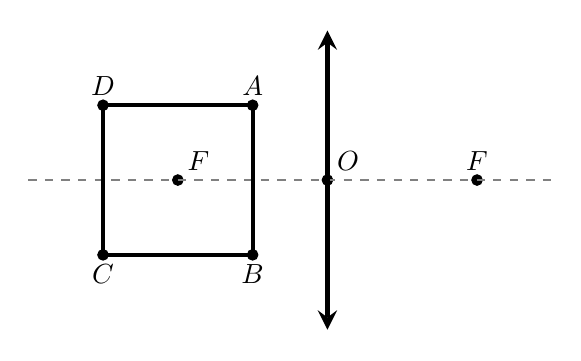
\begin{tikzpicture}[scale=0.95]
			\filldraw[black] (-2,0) circle (2pt) node[anchor=south west] {$F$};
			\filldraw[black] (2,0) circle (2pt) node[anchor=south] {$F$};
			\filldraw[black] (0,0) circle (2pt) node[anchor=south west] {$O$};
			\filldraw[black] (-1,1) circle (2pt) node[anchor=south] {$A$};
			\filldraw[black] (-1,-1) circle (2pt) node[anchor=north] {$B$};
			\filldraw[black] (-3,-1) circle (2pt) node[anchor=north] {$C$};
			\filldraw[black] (-3,1) circle (2pt) node[anchor=south] {$D$};
			\draw[gray] [dashed,-] (-4,0) -- (3,0);
			\draw[black, line width=1.5pt] (-1,1) -- (-1,-1);
			\draw[black, line width=1.5pt] (-1,-1) -- (-3,-1);
			\draw[black, line width=1.5pt] (-3,-1) -- (-3,1);
			\draw[black, line width=1.5pt] (-3,1) -- (-1,1);
			\draw[line width=2pt,>=stealth, <->] (0,-2) -- (0,2);
		\end{tikzpicture}
	\end{figure}
	
	
	\vspace{-10pt}
\probend
\bigskip

% Ü25
\setAuthor{}
\setRound{piirkonnavoor}
\setYear{2020}
\setNumber{G 2}
\setDifficulty{2}
\setTopic{TODO}

\prob{Karussell}
Juku läheb lõbustusparki ja märkab tiirlevat karusselli. Karussell koosneb ringikujulisest horisontaalsest kettast, mille küljes ripuvad kettide otsas lõbusõitjad. Juku märkab, et kinnitusketid moodustavad karusselli täiskiirusega pöörlemisel vertikaali suhtes nurga $\theta = \SI{60}{\degree}$.  Leia lõbusõitjate joonkiirus, kui karussell pööreleb täiskiirusel. Mitu tiiru minutis teeb karussell täiskiirusega pööreldes? Karusselli ketta raadius $R=\SI{10}{m}$, kettide pikkus $l=\SI{2}{m}$, raskuskiirendus $g=\SI{9,8}{m / s^2}$. Kettide kaalu mitte arvestada.
\probend
\bigskip

% Ü26
\setAuthor{}
\setRound{lõppvoor}
\setYear{2020}
\setNumber{G 2}
\setDifficulty{2}
\setTopic{TODO}

\prob{Kohukesed}
Richard ostis kohukesi, mis on ühtlase kihina poekoti põhjas. Heatujulisena teeb
ta kotiga vertikaalseid ringe, aga siis hakkab kohukeste pärast muretsema. Õnneks
selgub, et need ei kukkunud välja ja lömaks ka ei läinud. Näidake, et kui Richard
kotiga ei vehi (ega seda keeruta), siis võib ta panna koti põhja kaks korda
paksema kihi kohukesi, ilma et ükski kohuke lömastuks. Kohukesi võib käsitleda
vedelikuna. Võib eeldada, et kohuke lömastub siis, kui rõhk tema juures ületab
mingi kriitilise väärtuse. Vertikaalsete ringide tegemisel on Richardi käe
nurkkiirus konstantne. Eeldada, et kohukeste kihi paksus on palju väiksem kui
ringi raadius.
\probend
\bigskip

% Ü27
\setAuthor{Eero Vaher}
\setRound{lahtine}
\setYear{2021}
\setNumber{G 2}
\setDifficulty{2}
\setTopic{TODO}

\prob{Plokk}
Ideaalsel plokil on kaks raskust massidega $m$ ning $M=3m$. Väiksem raskus on maapinnal, suuremat raskust hoitakse kõrgusel $H$ nii, et raskusi ühendav venimatu nöör on pingul. Kui suurem raskus lahti lastakse hakkab süsteem raskusjõu mõjul vabalt liikuma. Mis on suurim kõrgus $h_\text{max}$, milleni väiksem raskus liikumise käigus tõuseb? Raskuskiirendus on $g$ ning nöör on piisavalt pikk, et väiksem raskus plokini ei jõua.
\probend
\bigskip

% Ü28
\setAuthor{Kaur Aare Saar}
\setRound{piirkonnavoor}
\setYear{2021}
\setNumber{G 2}
\setDifficulty{2}
\setTopic{TODO}

\prob{Klaaspudel}
Klaaspudel ruumalaga $V_0=\SI{1}{\liter}$ on osaliselt täidetud veega, mis on temperatuuril $T_0=\SI{20}{\celsius}$. Algul on pudelis olev rõhk võrdne välise rõhuga, mis on $p_0=\SI{100}{\kilo\pascal}$. Pudel suletakse ja pannakse sügavkülma nii, et seal olev vesi hakkab jäätuma. Pudel kannatab maksimaalset ülerõhku $\Delta p=\SI{300}{\kilo\pascal}$. Leidke maksimaalne kogus vett $V_{\text{v}}$, mis võis alguses pudelis olla, et pudel ei läheks vee jäätumisel katki. Vee tihedus lugeda kõikidel temperatuuridel võrdseks $\rho_{\text{v}}=\SI{1000}{\kilo\gram\per\meter\cubed}$ ja jää tihedus on $\rho_{\text{j}}=\SI{920}{\kilo\gram\per\meter\cubed}$. Eeldage, et pudelis olev õhk ja vesi on soojuslikus tasakaalus terve protsessi vältel ja et juurde tekkiv jää saab vabalt liikuda pudeli õhuga täidetud osasse.

\emph{Vihje.} Pudelis olevat õhku võib käsitleda kui ideaalset gaasi, mille rõhk $p$, ruumala $V$ ja absoluutne temperatuur $T$ (mida SI süsteemis mõõdetakse kelvinites) rahuldavad seost $\tfrac{pV}{T}=\textit{const}$.
\probend
\bigskip

% Ü29
\setAuthor{Jarl Patrick Paide}
\setRound{lõppvoor}
\setYear{2021}
\setNumber{G 2}
\setDifficulty{2}
\setTopic{TODO}

\prob{Pudel}
Pärast kuumal päeval õues treenimist tuli sportlane oma tühja õrnast plastmassist joogipudeliga jahedasse tuppa ning ta märkas, et ta pudel hakkas vaikselt \enquote{paukuma}. Lähemal uurimisel selgus, et kui pudeli sisene rõhk erineb välisest rõhust suuruse $\Delta p$ võrra, siis tekib pudeli kesta sisse üks lohukujuline mõlk juurde (selle tekkimine kostuski pauguna) ning hetkeks võrdsustuvad sise- ja välisrõhud. Sportlane mõõtis kahe paugu vaheliseks ajaks $t$. Leidke pudeli soojuskadude võimus vahetult pärast pudeli tuppa toomist. Tühja pudeli (seal hulgas pudelis oleva õhu) soojusmahutavus on $c$, õhu molaarruumala on $V_m$ ja universaalne gaasikonstant on $R$. Võib eeldada, et ajavahemiku $t$ jooksul soojuskadude võimus ei muutu.
\probend
\bigskip

% Ü30
\setAuthor{Joonas Kalda}
\setRound{lahtine}
\setYear{2022}
\setNumber{G 2}
\setDifficulty{2}
\setTopic{TODO}

\prob{Pliiats}
\begin{wrapfigure}{r}{0.1\textwidth}
\raisebox{3pt}[\dimexpr\height-0.6\baselineskip\relax]{\includegraphics[scale=0.95]{2022-lahg-02-yl.pdf}}
\vspace{-55pt}
\end{wrapfigure}
Pliiatsi kahe näpu vahel õhus hoidmiseks tuleb rakendada sama jõudu olenemata sellest, kas hoitakse kinni tipust või külje pealt. Näpu hõõrdetegurid pliiatsi küljega ja teritatud osaga on vastavalt $\mu_1 = \SI{0,3}{}$ ja $\mu_2 = \SI{0,5}{}$. Milline on pliiatsi tipunurk $\alpha$?
\probend
\bigskip

% Ü31
\setAuthor{Jaan Kalda}
\setRound{piirkonnavoor}
\setYear{2022}
\setNumber{G 2}
\setDifficulty{2}
\setTopic{TODO}

\prob{Juhe}
Peeter tahab vältida kasvuhoones taimede külmumist ja viib sinna elektriradiaatori nimivõimsusega $P=\qty{2}{\kW}$ ja nimipingega $V_0=\qty{230}{\V}$. Ta kasutab selleks pikendusjuhet pikkusega $L=\qty{40}{\m}$, mis  sisaldab kahte kõrvuti paiknevat vasktraati ristlõikepindalaga $S=\qty{1}{\mm\squared}$. Vase eritakistus $\rho=\qty{17}{\mohm\mm\squared\per\m}$. Milline soojuslik võimsus eraldub juhtmetes, kui tegelik võrgupinge pistikus on $V_p=\qty{240}{V}$?
\probend
\bigskip

% Ü32
\setAuthor{Moorits Mihkel Muru}
\setRound{lõppvoor}
\setYear{2022}
\setNumber{G 2}
\setDifficulty{2}
\setTopic{TODO}

\prob{Lumeväli}
Mari on kooli hiljaks jäämas ning proovib välja arvutada, kuidas joosta üle kooli ees oleva väljaku, mis on lumega kaetud. Väljak on ristkülikukujuline, mille ühes tipus asub Mari ja diagonaali teises tipus koolimaja uks. Väljaku koolimaja fassaadiga parallelne külg on \SI{100}{\metre} pikk ja koolimajaga risti olev külg \SI{50}{\metre}. Mari jookseb mööda teed kiirusega \SI{6}{\metre\per\second}, ja ta hindab, et ta jookseb lumes 20\% aeglasemalt kui mööda väljaku ääres olevat teed. Kui palju aega on võimalik Maril säästa joostes üle lumise väljaku võrreldes sellega, kui ta jookseks mööda väljaku ääres olevat teed?
\probend
\bigskip

% Ü33
\setAuthor{Richard Luhtaru}
\setRound{lahtine}
\setYear{2023}
\setNumber{G 2}
\setDifficulty{2}
\setTopic{TODO}

\prob{Kumerpeegel}
Joonisel (suurendatult lisalehel) on kujutatud ese AB ja kumerpeegel, mille keskpunkt on O ja fookus on F. Eeldame, et ese on sümmeetriateljest natuke nihkes, nii et see on punktist P nähtav nii otse kui kumerpeeglis. Mitu korda väiksem paistab ese AB punktist P kumerpeegli abil vaadelduna (võrreldes otse vaatamisega)? Lahendage ülesanne lisalehel.

\begin{figure}[h]
    \centering

    \includegraphics[width=0.75\linewidth]{2023-lahg-02-yl.png}
     \vspace{-20pt}
\end{figure}
\probend
\bigskip

% Ü34
\setAuthor{Konstantin Dukatš}
\setRound{piirkonnavoor}
\setYear{2023}
\setNumber{G 2}
\setDifficulty{2}
\setTopic{TODO}

\prob{Otsene kalorimeetria}
Üks viis, kuidas mõõta inimeselt või loomalt eralduva soojuse võimsust, on otsene kalorimeetria. Selle käigus pannakse inimene soojusisolatsiooniga tuppa, kus tagatakse inimese jaoks vajalik õhuvahetus. Kehast eralduva soojushulga leidmiseks läbib tuba veetoru, milles oleva vee temperatuur mõõdetakse enne ja pärast toa läbimist. Eeldage, et vesi siseneb tuppa temperatuuril $T_1 = \SI{20.00}{\celsius}$ ning väljub temperatuuril $T_2 = \SI{20.15}{\celsius}$. Vee kiirus torus on $u = \SI{2}{\meter\per\second}$ ja toru ristlõikepindala on $S=\SI{1}{\cm\squared}$. Mis on inimese kehast eralduva soojuse võimsus $P$? Vee tihedus on $\rho = \SI{1000}{\kg\per\meter\cubed}$ ning vee erisoojus on $c = \SI{4200}{\joule\per\kilogram\per\celsius}$. Võib eeldada, et õhuvahetuse käigus soojusvahetust ei toimu ning süsteem on termodünaamilises tasakaalus.
%(NB! Vana versiooni tõlge, eestikeelne tekst on uuendatud) Одним из способов определения количества тепла, выделенного организмом человека или животного является прямая калориметрия. Представим, что человека поместили в теплоизолированную комнату, в которую подается О$_2$ и поглощается избыток СО$_2$ и водяных паров. Продуцируемое организмом человека тепло измеряют с помощью термометров по нагреванию воды, протекающей по трубкам в камере. Вода температуры $T_1 = 20.00 \degree C $ входит в камеру, а выходит с температурой $T_2 = 20.15 \degree C $. Высота между поверхностью воды в бассейне до входа в камеру и краном после выхода постоянна и равна $h = 0.2$m, площадь поперечного сечения трубы $S=1$ cm$^2$. Чему равна мощность $P$ выделения тепла человеком?
\probend
\bigskip

% Ü35
\setAuthor{Jaan Kalda}
\setRound{lõppvoor}
\setYear{2023}
\setNumber{G 2}
\setDifficulty{2}
\setTopic{TODO}

\prob{Elektrikarjus}
Elektrikarjusega karjatamisel ümbritseb karjamaad pikk traat, mis on postide abil maast elektriliselt isoleeritud. Elektrikarjuses olev generaator saadab sellesse traati impulsspinge: pingevabad perioodid vahelduvad lühikeste pingega perioodidega. Pingeimuplsi ajal võib elektrikarjuse pingegeneraatorit vaadelda kui elektromotoorjõudu $\mathcal E$, mis omab teatud sisetakistust $R$. Elektriimpulss on eluohtlik, kui inimest läbib vool, mis on suurem kui $I_0=\SI{30}{mA}$. Teatud marki elektrikarjuse kohta on teada järgmist: kui pingegeneraatori väljundklemmidest üks on maandatud ja teisest lähtuv karjaaia traat on maapinnast ideaalselt isoleeritud, siis traadi ja maapinna vaheline pinge on impulsi ajal $U_m=\SI{15}{kV}$. Inimene, kes kõnnib paljajalu ja on seetõttu heas elektrilises kontaktis maapinnaga, puudutab kuiva käega karjuse traati ning saab elektrilöögi. Eeldage, et inimese keha takistus on hulga väiksem, kui kuiva käenaha takistus $r=\SI 5\kohm$.\\
\osa Joonistage elektriskeem, mis kirjeldab olukorda, kui inimene saab parajasti karjuselt elektrilööki.\\
\osa Millised sisetakistuse $R$ väärtused on lubatavad?
\probend
\bigskip

% Ü36
\setAuthor{Jarl Patrick Paide}
\setRound{lahtine}
\setYear{2024}
\setNumber{G 2}
\setDifficulty{2}
\setTopic{TODO}

\prob{Kaks kera}
Kaks sama tiheduse ja ühtlase massijaotusega kera peaaegu puutuvad üksteist (keskpunktide vaheline kaugus on kaks raadiust), aga hõõrdumist ei toimu. Kerad tiirlevad ümber üksteise gravitatsioonijõu tõttu nurkkiirusega $\omega$. Leia kerade tihedus.
\probend
\bigskip

% Ü37
\setAuthor{Moorits Mihkel Muru}
\setRound{piirkonnavoor}
\setYear{2024}
\setNumber{G 2}
\setDifficulty{2}
\setTopic{TODO}

\prob{Hajumine}
Juhanil on valgusallikas, mis tekitab paralleelset silindrikujulist valgusvihku, ning väike fotodetektorist tajur, mis mõõdab valguse intensiivsust. Esimeses katses mõõdab Juhan valgusallika intensiivsust, asetades tajuri täielikult valgusallika valgusvihku (ilma kumerpeeglita). Teises katses (vt joonis) suunab Juhan valgusvihu kumerpeeglile, mille kumerusraadius on $R=\SI{30}{\centi\m}$, nii et valgusvihk asub optilisel peateljel ja on sellega paralleelne. Seejärel mõõdab Juhan hajunud valguse intensiivsust, asetades tajuri täielikult peegeldunud valgusvihku (aga valgusallika enda valgusvihust kõrvale) peegli pinnast $L=\SI{60}{\centi\m}$ kaugusele. Mitu korda on tajuri näit esimeses katses suurem kui teises katses? Võib eeldada, et valgusallika valgusvihu laius on palju väiksem peegli kumerusraadiusest.

\begin{figure}[h]
    \centering
    \includegraphics[width=0.6\linewidth]{2024-v2g-02-yl.png}
\end{figure}
\probend
\bigskip

% Ü38
\setAuthor{Taavi Pungas}
\setRound{lõppvoor}
\setYear{2024}
\setNumber{G 2}
\setDifficulty{2}
\setTopic{TODO}

\prob{Ragulka}
Eva leidis pargist ragulka ning soovis sellega lasta kivikese vertikaalselt üles nii, et see täpselt puudutaks tema kohal asuvat puuoksa. Kui Eva venitab ragulka kummi lõdvast olekust \SI{3}{\cm} kaugusele, siis jääb kivil puudu $1/4$ vahemaast oksani. Kui kaugele peaks Eva venitama ragulka kummi, et kivike jõuaks täpselt oksani?
\probend
\bigskip

% Ü39
\setAuthor{Jaan Kalda}
\setRound{lahtine}
\setYear{2018}
\setNumber{G 3}
\setDifficulty{3}
\setTopic{TODO}

\prob{Ring}
Traadist, mille ühe detsimeetri takistus on üks oom tehakse ring ümbermõõduga kuus detsimeetrit. Iga detsimeetri järel märgitakse punktid $a, b, \ldots, f$. Punktide $a$ ja $e$ vahele ühendatakse patarei pingega \SI{7}{V}, punktide $d$ ja $f$ vahele ampermeeter ning $d$ ja $b$ vahele voltmeeter. Punktid $f$ ja $b$ ühendatakse samast traadist lõigatud kahe-detsimeetrise traadijupiga. Leidke ampermeetri ja voltmeetri näidud.
\probend
\bigskip

% Ü40
\setAuthor{Hans Daniel Kaimre}
\setRound{lahtine}
\setYear{2019}
\setNumber{G 3}
\setDifficulty{3}
\setTopic{TODO}

\prob{Lääts}
Optiline süsteem koosneb punktvalgusallikast ja ekraanist, mille vahele on asetatud õhuke koondav lääts. Ekraani ja valgusallika vaheline kaugus on $L$. Millist tingimust peab rahuldama läätse fookuskaugus, et ekraanile tekiks tõeline kujutis? Kui fookuskaugus on võimalikult suur, siis milline on optilise süsteemi suurendus?
\probend
\bigskip

% Ü41
\setAuthor{}
\setRound{piirkonnavoor}
\setYear{2019}
\setNumber{G 3}
\setDifficulty{3}
\setTopic{TODO}

\prob{Kärbes}
Kärbes asub kumerläätsest kümnekordse fookuskauguse kaugusel ning läätse optilisest peateljest kolme fookuskauguse kaugusel ning hakkab liikuma otse oma kujutise poole. Kui kaugel läätse tasandist asub kärbes hetkel, kui tema tõeline kujutis liigub kärbse suhtes\\
\osa kõige aeglasemalt;\\
\osa kõige kiiremini? Kui suur on kärbse kujutise kiirus kärbse suhtes nendel hetkedel? Põhjendage vastust.
\probend
\bigskip

% Ü42
\setAuthor{}
\setRound{lõppvoor}
\setYear{2019}
\setNumber{G 3}
\setDifficulty{3}
\setTopic{TODO}

\prob{Lennuk}
\begin{wrapfigure}[12]{r}{0.37\textwidth}
  \vspace{-28pt}
  \begin{center}
  \includegraphics[scale=0.2]{2019-v3g-03-yl.png}
  \end{center}
  \vspace{-20pt}
\end{wrapfigure}


Joonisel on lennuki algne asukoht märgitud ristiga. Iga tunni järel mõõdeti lennuki kaugust fikseeritud punktist. Saadud kaugused on joonisel märgitud ringjoonena mõõtepunkti ümber. Konstrueerige kõikvõimalikud lennuki trajektoorid $\SI{7}{h}$ jooksul, kui on teada, et pärast starti lendas lennuk $\SI{4}{h}$ otse, muutis seejärel suunda ning lendas ülejäänud aja samuti otse. Eeldada, et lennuki kiirus maapinna suhtes oli ühtlaselt $\SI{500}{km/h}$. Lahendus esitada lisalehel.
\textit{Märkus.} Suuna muutus võis olla ka väga väike.
\probend
\bigskip

% Ü43
\setAuthor{Hans Daniel Kaimre}
\setRound{lahtine}
\setYear{2020}
\setNumber{G 3}
\setDifficulty{3}
\setTopic{TODO}

\prob{U-klaas}
\begin{wrapfigure}[6]{r}{0.25\linewidth}
		\vspace{-10pt}
		\includegraphics[width=\linewidth]{2020-lahg-03-yl.pdf}
	\end{wrapfigure}
	U-kujulise klaastüki (vt joonist) ristlõige on ristkülik. Tahule A langeb selle pinnaga risti paralleelne valgusvihk.  Millist tingimust peaks rahuldama sisemise külje kõverusraadius $R$, et kogu pealelangev valgus väljuks tahust B? Struktuuri laius $d=\SI{3}{\cm}$, klaasi murdumisnäitaja $n=\num{1.5}$ ning tahud A ja B on kaetud peegeldumisvastase kilega.
\probend
\bigskip

% Ü44
\setAuthor{}
\setRound{piirkonnavoor}
\setYear{2020}
\setNumber{G 3}
\setDifficulty{3}
\setTopic{TODO}

\prob{Hüppav silinder}
\begin{wrapfigure}[10]{r}{0.3\textwidth}
    \vspace{-30pt}
	\includegraphics[width=0.3\textwidth]{2020-v2g-03-yl.pdf}
\end{wrapfigure}


Peenike seest tühi silinder on nööriga kinnitatud veega täidetud basseini põhja nii, nagu näidatud joonisel. 
Silindri ülemine ots asub veepinnal. Nöör lõigatakse läbi ja silinder hakkab ülespoole liikuma ning hüppab veest välja. Kui kõrgele õhku tõuseb silindri alumine ots veepinnast maksimaalselt? Eeldage, et veest täielikult väljumise hetkel läheb 50\% silindri kineetilisest energiast kaduma silindri ja veepinna vastastikmõju tõttu. Muude keskkonna takistusjõududega ei pea arvestama.
Silindri mass $m = \SI{30}{g}$, raadius $r = \SI{1}{cm}$ ja kõrgus $h = \SI{0.5}{m}$. Vee tihedus $\rho_v=\SI{1000}{kg/m^3}$.
\probend
\bigskip

% Ü45
\setAuthor{}
\setRound{lõppvoor}
\setYear{2020}
\setNumber{G 3}
\setDifficulty{3}
\setTopic{TODO}

\prob{Käivitusvool}
\begin{wrapfigure}{r}{0.35\textwidth}
  \vspace{-25pt}
  \begin{center}
  \includegraphics[scale=0.6]{2020-v3g-03-yl.pdf}
  \vspace{-20pt}
  \end{center}
\end{wrapfigure}
Taavet otsustas ära mõõta auto käivitusvoolu tugevuse. Ta leidis ampermeetri
mõõtepiirkonnaga~$I_0=\SI{1}{\milli\ampere}$ ja sisetakistusega~$R_0=\SI{100}{\ohm}$
ja paraja pikkusega jupi vasktoru, mille sisediameeter oli
$d_1=\SI{6}{\milli\meter}$ ja välisdiameeter $d_2=\SI{8}{\milli\meter}$. Ta ühendas
vasktoru jadamisi autoaku ja starteriga (mida võib käsitleda kui takistit) ning ampermeetri rööbiti
vasktoruga nagu kujutatud kõrvaloleval skeemil. Milline tuleks
valida kontaktide vaheline distants~$\ell$, et ampermeetri maksimaalsele
näidule~$I_0$ vastaks mõõdetava voolu suurus $I_1=\SI{500}{\ampere}$?
Vase eritakistus on $\rho=\SI{1.68e-8}{\ohm\meter}$. Ühendusjuhtmete ja
-kontaktide takistused võib lugeda tühiseks.
\probend
\bigskip

% Ü46
\setAuthor{Konstantin Dukatš}
\setRound{lahtine}
\setYear{2021}
\setNumber{G 3}
\setDifficulty{3}
\setTopic{TODO}

\prob{Kumerpeegel}
Joonisel on kujutatud kumerlääts, selle optiline peatelg ning üks fookustest. On teada, et kusagil optilises skeemis leidub ka kumerpeegel. Kui panna valgusallikas punktidesse $S_1$ või $S_2$, siis tekkinud kujutis kattub allikaga. Konstrueerige kumerpeegel. Esitage lahendus lisalehel.
\begin{figure}[h]
  \vspace{-1em}
  \centering
  \resizebox{\textwidth}{!}{%
  \begin{tikzpicture}[scale=1]
    \filldraw[black] (2,0) circle (1.5pt) node[anchor=south] {$F$};
    \filldraw[black] (0,0) circle (1.5pt) node[anchor=south west] {$O$};
    \filldraw[black] (-3.6,0) circle (1.5pt) node[anchor=south] {$S_2$};
    \filldraw[black] (-6,0) circle (1.5pt) node[anchor=south] {$S_1$};


    \draw[gray] [dashed,-] (-7,0) -- (7,0);
    \draw[line width=1pt,Stealth-Stealth] (0,-2) -- (0,2);
  \end{tikzpicture}
  }%
  \vspace{-1em}
\end{figure}
\probend
\bigskip

% Ü47
\setAuthor{Kaarel Hänni}
\setRound{piirkonnavoor}
\setYear{2021}
\setNumber{G 3}
\setDifficulty{3}
\setTopic{TODO}

\prob{Joogid}
Kauril on 3 anumat, igas neist on võrdselt $\SI{1}{\kilo\gram}$ vett. Anumates oleva vee temperatuurid on vastavalt $\SI{10}{\celsius}$, $\SI{20}{\celsius}$ ja $\SI{30}{\celsius}$.
% Lisaks on Kauril mõõdukann ja palju anumaid.
Kas Kauril on võimalik vaid antud vedelikke segades \\
\osa teha $2$ jooki, kumbki massiga $\SI{1.5}{\kilo\gram}$ ja temperatuuridega vastavalt $\SI{13}{\celsius}$~ja~$\SI{27}{\celsius}$;\\
\osa teha $5$ jooki, igaüks massiga $\SI{0.5}{\kilo\gram}$ ja temperatuuridega vastavalt $\SI{12}{\celsius}$,~$\SI{17}{\celsius}$,~$\SI{18}{\celsius}$,~$\SI{20}{\celsius}$~ja~$\SI{22}{\celsius}$?\\
Eeldage mõlema puhul, et soojusvahetust keskkonnaga ei toimu.
\probend
\bigskip

% Ü48
\setAuthor{Oleg Košik}
\setRound{lõppvoor}
\setYear{2021}
\setNumber{G 3}
\setDifficulty{3}
\setTopic{TODO}

\prob{Lääts ja ekraan}
Jarl asetas punktvalgusallika ja ekraani vahele õhukese kumerläätse (raamita klaaslääts); valgusallikas asus peateljel ja ekraani tasand oli paralleelne läätse tasandiga. Ta liigutas ekraani edasi-tagasi, uurides sellel tekkivat mustrit ning pani tähele, et kui ekraan asub läätsest kaugusel \SI{10}{\cm}, tekib ekraanile terav valgusallika kujutis. Üllatuslikult selgus, et kui ekraani kaugus läätsest oli \SI{60}{\cm}, siis ei olnud seal näha enam mingit mustrit: ekraan oli ühtlase heledusega nagu läätse polnukski!\\
\osa Leidke läätse fookuskaugus.\\
\osa Mis kujuga muster tekib ekraanile, kui ekraan asub kaugemal, kui \SI{10}{\cm} läätsest, kuid lähemal, kui \SI{60}{\cm} läätsest?
\probend
\bigskip

% Ü49
\setAuthor{Kaarel Hänni}
\setRound{lahtine}
\setYear{2022}
\setNumber{G 3}
\setDifficulty{3}
\setTopic{TODO}

\prob{Kõnd eskalaatoril}
\begin{wrapfigure}{r}{0.16\textwidth}
\raisebox{-5pt}[\dimexpr\height-0.6\baselineskip\relax]{
  \begin{tikzpicture}
    \draw (0,0) rectangle (2,2.5);
    \draw[pattern={Lines[angle=55,distance=10pt]}] (0,2.5) rectangle (2,5);
    \draw (2.3,2.5) node {$a$};
    \draw (1,-0.3) node {$b$};
  \end{tikzpicture}
}
\end{wrapfigure}

Sandra eesmärk on kõndida ristkülikukujulise koridori alumisest vasakust nurgast ülemisse paremasse nurka. Koridor on piklik ristkülik  (pealtvaade joonisel) pikkusega $a = \SI{200}{m}$ ja laiusega $b = \SI{4}{m}$. Enda aitamiseks saab ta koridori ülemise poole põranda asendada vabalt valitud suunas liikuva lindiga (nagu tihti lennujaamades olevad horisontaalsed eskalaatorid). Sandra soovib lindi liikumissuuna valida selliselt, et ta saab võimalikult kiiresti koridori alumisest vasakust nurgast koridori ülemisse paremasse nurka jõuda. Millise nurga all koridori vasakpoolse küljega peaks Sandra lindi liikumissuuna valima? Sandra kõnnib enda all oleva pinna suhtes maksimaalse kiirusega $v = \SI{2}{\meter \per \second}$, lint liigub maksimaalse kiirusega $u = \SI{3}{\meter \per \second}$.\\
\emph{Märkus:} kui $x \approx 0$, siis võib kasutada lähendusi $\sqrt{1+x} \approx 1 + \frac{x}{2}$ ja $\sin{x} \approx \tan{x} \approx x$ (nurk $x$ on radiaanides).
\probend
\bigskip

% Ü50
\setAuthor{Kaarel Kivisalu}
\setRound{piirkonnavoor}
\setYear{2022}
\setNumber{G 3}
\setDifficulty{3}
\setTopic{TODO}

\prob{Liumägi}
Liumägi koosneb kahest osast: kaldpind nurgaga $\alpha$ ja horisontaalne pind. Liumäe kõrgus on $h$ ja horisontaalne pikkus on $l$ (vt joonist). Liumägi tahetakse teha selline, et sealt alla lastes jõuaks täpselt liumäe lõppu, aga jäädes lõpus paigale. Võib eeldada, et üleminek kaldpinnalt horisontaalsele pinnale on sujuv. Milline peaks olema sellise liumäe jaoks hõõrdetegur $\mu$ liumäe ja allalaskja vahel?
\begin{figure}[h]
  \vspace{-1.5em}
  \centering
  {
    \tikzset{component/.style={draw,thick,circle,fill=white,minimum size=0.75cm,inner sep=0pt}}
    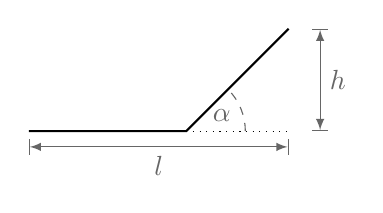
\begin{tikzpicture}
      %lines
      \draw[thick] (0,0) -- (2,0) -- (3.3,1.3);
      \draw[dotted] (2,0) -- (3.3,0);
      %angle
      \draw[dashed, black!60] (2.75,0) arc (0:45:.75);
      \draw[black!60] (2.45,0.2) node {$\alpha$};
      %lenghts
      \draw[|<->|, >=latex, black!60] (3.7,0)-- (3.7,1.3) node[midway, right]{$h$};
      \draw[|<->|, >=latex, black!60] (0,-0.2)-- (3.3,-0.2) node[midway, below]{$l$};
    \end{tikzpicture}
  }
  \vspace{-2em}
\end{figure}
\probend
\bigskip

% Ü51
\setAuthor{Richard Luhtaru}
\setRound{lõppvoor}
\setYear{2022}
\setNumber{G 3}
\setDifficulty{3}
\setTopic{TODO}

\prob{Silinder}
\begin{wrapfigure}{r}{5cm}
  \vspace{-2em}
  \begin{center}
    \includegraphics[width=\linewidth]{2022-v3g-03-yl.pdf}
  \end{center}
  \vspace{-2em}
\end{wrapfigure}

Õhukese silindri eritakistus on $\rho$, raadius on $r$, kõrgus on $h$ ja paksus on $\tau$. Silindri ringikujulised põhjad on eemaldatud ning silindri vastaspooltel on silindri materjal asendatud peenikeste juhtivate klemmidega, mille pikkus on $h$ ja paksus on $\tau$ (A ja B joonisel). Leidke kahe klemmi vaheline takistus.
\probend
\bigskip

% Ü52
\setAuthor{Valter Kiisk}
\setRound{lahtine}
\setYear{2023}
\setNumber{G 3}
\setDifficulty{3}
\setTopic{TODO}

\prob{Kummipael}
\begin{wrapfigure}[8]{r}{0.5\linewidth}
    %\vspace{-10pt}
    \begin{center}
        \vspace{5pt}
        \includegraphics[width=\linewidth]{2023-lahg-03-yl.pdf}
    \end{center}
\end{wrapfigure}


Kummipaela pikkus vabas olekus on $L=\SI{15}{cm}$. Kui kummipaela külge riputati tundmatu massiga koormis, siis kummipaela pikkus kasvas $\Delta L=\SI{2}{cm}$ võrra (vt joonis). Seejärel kummipael fikseeriti otstest kahe samal kõrgusel paikneva punkti vahele, mille vahekaugus oli $2L$ (st pael venitati $L$ võrra pikemaks). Sama koormis riputati nüüd kummipaela keskpunkti. Hinnake, kui suur on selle punkti läbivajumine. Võib eeldada, et kummipaelas tekkiv elastsusjõud on võrdeline pikenemisega ja kummipaela enda mass on tühine.\\ \emph{Märkus:} Väikeste nurkade $x$ korral võib kasutada lähendust $\sin{x} \approx \tan{x} \approx x$ (nurk $x$ on radiaanides).
\probend
\bigskip

% Ü53
\setAuthor{Marten Rannut}
\setRound{piirkonnavoor}
\setYear{2023}
\setNumber{G 3}
\setDifficulty{3}
\setTopic{TODO}

\prob{Ökonoomne sõit}
Linnas kiirendab sisepõlemismootoriga auto tippkiiruseni $\SI{40}{\km\per\hour}$ ning peab peatuma keskmiselt iga $100$ meetri tagant. Linnasõidul võib õhutakistust mitte arvestada. Maanteel sõidab auto püsiva kiirusega $\SI{90}{\km\per\hour}$. Õhutakistusjõud avaldub kujul $F=cv^2$, kus $c = \SI{1.3}{\kg\per\meter}$ ja $v$ on auto kiirus. Auto kaalub $\num{1.5}$ tonni. Leidke maanteesõidu ja linnasõidu kütusekulude suhe $\SI{100}{\km}$ sõidu kohta. Eeldage, et mootori kasutegur ei sõltu kiirusest ja kiirendusest.
\probend
\bigskip

% Ü54
\setAuthor{Aigar Vaigu}
\setRound{lõppvoor}
\setYear{2023}
\setNumber{G 3}
\setDifficulty{3}
\setTopic{TODO}

\prob{Lääts ja kaks peeglit}
Konstrueerige objekti $AB$ (vt joonist lisalehel) kõik kujutised. Skeemil on hall sein, sinine \SI{45}{\degree} kaldu poolläbilaskev peegel (pool valgusest läheb otse läbi, pool peegeldub nagu tavalises tasapeeglis), kumerlääts fookuskaugusega $f$ ja tasapeegel. Lahendage ülesanne lisalehel.
\probend
\bigskip

% Ü55
\setAuthor{Richard Luhtaru}
\setRound{lahtine}
\setYear{2024}
\setNumber{G 3}
\setDifficulty{3}
\setTopic{TODO}

\prob{Valguskaabel}
Silindriline sirge valguskaabel koosneb südamikust ja kattekihist ning selle ots on tasane ja kaabliga risti. Kui valgustada kaabli otsa välise valgusallikaga, siseneb osa välisest valgusest südamikku ja levib praktiliselt kadudeta pikki vahemaid. Seda, kui vastuvõtlik on valguskaabel välisele valgusele, iseloomustab numbriline apertuur (NA), mis on defineeritud kui $\text{NA} = \sin \theta_0$, kus $\theta_0$ on suurim välise valguskiire nurk (kaabli sümmeetriatelje suhtes), mis valguskaablisse sisenedes levib selle südamikus kadudeta. Leia valguskaabli numbriline apertuur NA, kui südamiku murdumisnäitaja on $n_1$, kattekihi murdumisnäitaja on $n_2$ ja kaabel asub välises keskkonnas murdumisnäitajaga $n_0$.
\begin{figure}[h]
    \centering
    \includegraphics[width=.7\linewidth]{2024-lahg-03-yl.pdf}
\end{figure}
\probend
\bigskip

% Ü56
\setAuthor{Hans Daniel Kaimre}
\setRound{piirkonnavoor}
\setYear{2024}
\setNumber{G 3}
\setDifficulty{3}
\setTopic{TODO}

\prob{Valgusdioodid}
\begin{wrapfigure}{r}{0.5\textwidth}
  \vspace{-30pt}
  \begin{center}
  \includegraphics[scale=0.8]{2024-v2g-03-yl.pdf}
  \vspace{-20pt}
  \end{center}
\end{wrapfigure}

Mari koostas patareist ning kahest valgusdioodist (LEDist) vooluringi (vt joonist), kuid vooluahela kokkuühendamisel valgusdioodid põlesid läbi ning purunesid. Mari küsis isalt nõu, kes soovitas lisada vooluringi üks takisti. Aidake Maril välja mõelda, kui suure väärtusega takisti ja kuidas peaks ta skeemi lisama, et valgusdioodid töötaks normaaltingimustel. Joonistage uus vooluahel ning arvutage sobiva takisti väärtus. Patarei klemmipinge $U=\SI{12}{\V}$, valgusdioodide nimipinged on vastavalt $U_1=\SI{3}{V}$ ja $U_2=\SI{3.5}{V}$ ning optimaalne voolutugevus normaaltingimustel töötamisel $I_1=I_2=\SI{30}{\milli\A}$.
\probend
\bigskip

% Ü57
\setAuthor{Sandra Schumann}
\setRound{lõppvoor}
\setYear{2024}
\setNumber{G 3}
\setDifficulty{3}
\setTopic{TODO}

\prob{Leedid}
Kadil on punane ja sinine valgusdiood, \SI{9}{\V} patarei, \SI{300}{\ohm} ja \SI{360}{\ohm} takistid ning punane ja sinine nupplüliti. Nupplülitil on kaks klemmi, mis on omavahel lühises, kui nupp alla vajutada, ja mis ei ole ühenduses, kui nuppu mitte vajutada. Punane diood süttib, kui talle rakendada päripinge \SI{1.8}{\V}, ja sinine, kui talle rakendada päripinge \SI{3}{\V}. Väiksematel pingetel dioode vool ei läbi. Pinge dioodidel ei sõltu teda läbiva voolu suurusest. Millise skeemi peab Kadi moodustama, et vajutades punast lülitit põleks punane diood, vajutades sinist lülitit põleks sinine diood, mitte kumbagi vajutades ei põleks kumbki diood ja mõlemat lülitit vajutades samuti ei põleks kumbki diood. Kadi tahab ka, et dioodi põlemisel läbiks seda vool tugevusega \SI{20}{\mA} ning patarei poleks kunagi lühises.
\probend
\bigskip

% Ü58
\setAuthor{Erkki Tempel}
\setRound{lahtine}
\setYear{2018}
\setNumber{G 4}
\setDifficulty{4}
\setTopic{TODO}

\prob{Kahurid}
Kahurist $A$ lastakse horisondi suhtes nurga $\alpha=\SI{30}{\degree}$ all lendu kuul algkiirusega $v_A=\SI{140}{m/s}$ kahuri $B$ suunas, mis on esimesest kahurist $l=\SI{1}{km}$ kaugusel samal tasapinnal. Sel hetkel, kui kuul on oma trajektoori kõrgeimas punktis, tulistatakse kahurist $B$ teine kuul, mis $t_1=\SI 5s$ pärast põrkub  esimese kuuliga. Millise algkiirusega tulistati kuul kahurist $B$? Õhutakistusega mitte arvestada; vabalangemise kiirendus $g\approx\SI{10}{m/s^2}$.
\probend
\bigskip

% Ü59
\setAuthor{Kaarel Hänni}
\setRound{lahtine}
\setYear{2019}
\setNumber{G 4}
\setDifficulty{4}
\setTopic{TODO}

\prob{Laetud tasand}
Ruumis on ühtlaselt laetud tasand ja paaritu arv võrdseid laenguid, mis ei asu tasandil. Tõesta, et tasandile mõjuv resultantjõud ei saa olla 0.
\probend
\bigskip

% Ü60
\setAuthor{}
\setRound{piirkonnavoor}
\setYear{2019}
\setNumber{G 4}
\setDifficulty{4}
\setTopic{TODO}

\prob{Vaakum}
Mõlemast otsast õhukindlalt suletud klaastoru pikkus $\ell=\SI{1}{m}$ ja sisediameeter $d=\SI{1}{cm}$. Õhurõhk $p=\SI{101.3}{kPa}$.\
\osa Kui palju tööd tuleb minimaalselt teha vaakumi tekitamiseks selles torus?\\
\osa Horisontaalse vakumeeritud toru ühes otsas on teraskuulike, mis saab l	ibiseda toru sees praktiliselt ilma hõõrdumiseta ja mille diameeter on võrdne toru sisediameetriga. Õnnetuse tõttu puruneb toru ots, mille lähedal kuulike paikneb  ja õhu surve paneb kuulikese liikuma vakumeeritud osa suunas. Kui suure kiiruse saavutab kuulike jõudes toru teise otsa? Terase tihedus on $\SI{7.9}{g/cm^3}$.
\probend
\bigskip

% Ü61
\setAuthor{}
\setRound{lõppvoor}
\setYear{2019}
\setNumber{G 4}
\setDifficulty{4}
\setTopic{TODO}

\prob{Konveier}
Sile metallplaat pikkusega $l$ sõidab konveieril. Konveier koosneb kahest osast ning kummalgi osal on oma sile konveierilint. Mõlema lindi pikkus on $x$, kuid esimene lint liigub kiirusega $v_1$ ning teine kiirusega $v_2$. Algasendis on plaat esimese lindi alguses nii, et plaat asub täielikult esimesel konveierilindil ning plaadi tagumine serv ühtib esimese lindi algusega. Lõppasendis on plaat teise lindi lõpus nii, et plaat asub täielikult teisel konveierilindil ning plaadi esimene serv ühtib teise lindi lõpuga. Leida aeg $t$, mis kulub plaadil algasendist lõppasendisse jõudmiseks. Hõõrdetegur plaadi ja esimese konveierilindi vahel on $\mu_{1}$ ning plaadi ja teise konveierilindi vahel $\mu_{2}$. Eeldada, et üleminekukohas on vahe konveierilintide vahel tühiselt väike ning aeg, mis kulub plaadi kiiruse muutumiseks üleminekukohas, on tühiselt väike võrreldes koguajaga.
\probend
\bigskip

% Ü62
\setAuthor{Richard Luhtaru}
\setRound{lahtine}
\setYear{2020}
\setNumber{G 4}
\setDifficulty{4}
\setTopic{TODO}

\prob{Noova}
\begin{wrapfigure}[12]{r}{0.15\linewidth}
		\vspace{10pt}
		\includegraphics[width=1.1\linewidth]{2020-lahg-04-yl.pdf}
	\end{wrapfigure}
	Hobiastronoom Jarl vaatleb teleskoobiga noovaplahvatust ja mõõdab ühe plahvatuse ainejäänuki kiirust. On teada, et ainejäänuki tegelik kiirus on $v$ ja nurk kiirusvektori ja vaatesihi vahel on $\theta$.
	
	Jarl teab varasemate mõõtmiste põhjal, et noova kaugus on $D$, kuid ta ei tea nurka $\theta$. Seetõttu eeldab Jarl, et ainejäänuk liigub vaatesihiga risti ning arvutab kauguse ja jäänuki nurga muutumise abil jäänuki näiva kiiruse $v'$.
	
	Leia Jarli poolt mõõdetav näiv kiirus $v'$, eeldusel et noova on väga kaugel ($vt \ll D$, kus $t$ on vaatluse aeg) ning et kosmoloogiline paisumine on tühine. Valguse kiirus on $c$. Kas on võimalik, et ainejäänuki näiv kiirus $v'$ on mingi $v$ ja $\theta$ väärtuse korral valguse kiirusest suurem, isegi kui $v < c$?
\probend
\bigskip

% Ü63
\setAuthor{}
\setRound{piirkonnavoor}
\setYear{2020}
\setNumber{G 4}
\setDifficulty{4}
\setTopic{TODO}

\prob{Elektriruut}
\begin{wrapfigure}[9]{r}{0.5\textwidth}
\hspace{10pt}
\begin{circuitikz}[scale=0.5]
  \tikzset{
    declare function={
      atan3(\a,\b)=ifthenelse(atan2(0,1)==90, atan2(\a,\b), atan2(\b,\a));},
    kinky cross radius/.initial=+.3cm,
    @kinky cross/.initial=+, kinky crosses/.is choice,
    kinky crosses/left/.style={@kinky cross=-},kinky crosses/right/.style={@kinky cross=+},
    kinky cross/.style args={(#1)--(#2)}{
      to path={
        let \p{@kc@}=($(\tikztotarget)-(\tikztostart)$),
            \n{@kc@}={atan3(\p{@kc@})+180} in
        -- ($(intersection of \tikztostart--{\tikztotarget} and #1--#2)!%
               \pgfkeysvalueof{/tikz/kinky cross radius}!(\tikztostart)$)
        arc [ radius     =\pgfkeysvalueof{/tikz/kinky cross radius},
              start angle=\n{@kc@},
              delta angle=\pgfkeysvalueof{/tikz/@kinky cross}180 ]
        -- (\tikztotarget)}}}
  \draw (0,0) to[short, *-*] (0,0) to[european resistor] (0,4) to[short, *-*] (0,4)
  to[european resistor] (0,8) to[short, *-*,l=1] (0,8) to[european resistor] (4,8)
  to[short, *-*] (4,8) to[european resistor] (8,8) to[short, *-*] (8,8) to[european resistor] (8,4) to[short, *-*] (8,4) to[european resistor] (8,0) to[short, *-*,l_=2] (8,0) to[european resistor] (4,0) to[short, *-*] (4,0) to[european resistor] (0,0);

  \node (a) at (-0.125,4) {};
  \node (b) at (8.125,4) {};
  \node (c) at (4,8.125) {};
  \node (d) at (4,-0.125) {};


  \draw (c) -- (d);
  \draw (a) to [kinky cross=(c)--(d), kinky crosses=left] (b);
  \end{circuitikz}
\end{wrapfigure}

Leidke takistus punktide 1 ja 2 vahel (vt. joonis). Kõigi takistite takistus on $R$.
\probend
\bigskip

% Ü64
\setAuthor{}
\setRound{lõppvoor}
\setYear{2020}
\setNumber{G 4}
\setDifficulty{4}
\setTopic{TODO}

\prob{Tasakaaluliikur}
\begin{wrapfigure}{r}{0.35\textwidth}
  \vspace{-5pt}
  \begin{center}
  \includegraphics[scale=0.1]{2020-v3g-04-yl.png}
  \end{center}
  \vspace{-25pt}
\end{wrapfigure}
Hannes massiga $m = \SI{75}{\kilo\gram}$ sõidab tasakaaluliikuriga  konarlikul
teel ühtlase kiirusega $v$. Konarliku tee profiili saab külgvaates lähendada
koosinuslainele amplituudiga~$A = \SI{60}{\milli\meter}$ ja
perioodiga~$\Delta x = \SI{6}{\meter}$. Tasakaaluliikuril on amortiseerimissüsteem,
mis koosneb $n=2$ rööbiti ühendatud vedrust jäikusega $k = \SI{900}{\newton\per\meter}$.
Leidke kiirus~$v$, mille juures Hannes võngub enim ehk tekib resonants.
Tasakaaluliikuri kaal on tühine. Kiirus $v$ on kiirus, mida näitaks
tasakaaluliikuril olev GPS seade, mitte ratta keerlemisel põhinev odomeeter.

\emph{Vihje:} Kui keha kiirendus $a$ ja kaugus tasakaalupunktist $y$ on seotud
võrdusega $a=-\omega^2 y$, kus $\omega$ on positiivne konstant, siis võngub keha
perioodiga~$\frac{2\pi}{\omega}$.
\probend
\bigskip

% Ü65
\setAuthor{Jaan Kalda}
\setRound{lahtine}
\setYear{2021}
\setNumber{G 4}
\setDifficulty{4}
\setTopic{TODO}

\prob{Kuiv õhk}
Talvel võib liigne kuivus toas probleeme tekitada: alla 20-protsendine suhteline niiskus ei mõju hästi inimese nahale ja limaskestadele. Eeldage, et välisõhk siseneb tuppa läbi ventilatsiooni ja toaõhk vahetub väljast tulnud õhuga ühe tunni jooksul peaaegu täielikult ning et toas hoitakse 20-kraadilist õhutemperatuuri. Millise välisõhu temperatuuri juures langeb toas suhteline niiskus alla 20\%, kui väljas on suhteline niiskus 80\%? Küllastunud auru rõhu sõltuvus temperatuurist on toodud graafikul.\\
\emph{Märkus:} suhteliseks niiskuseks nimetatakse õhus oleva veeauru osarõhu ja antud temperatuuri juures küllastunud veeauru osarõhu suhet.

\begin{figure}[h]
  \vspace{-1em}
  \centering
  \includegraphics[width=0.95\textwidth]{2021-lahg-04-yl.pdf}
  \vspace{-1em}
\end{figure}
\probend
\bigskip

% Ü66
\setAuthor{Kaido Reivelt}
\setRound{piirkonnavoor}
\setYear{2021}
\setNumber{G 4}
\setDifficulty{4}
\setTopic{TODO}

\prob{Batüskaaf}
Monika sõidab keset ookeanit batüskaafi ehk süvaveeliikuriga. Ühel hetkel
ütlesid üles batüskaafi mootorid, millega veepaakidest vett välja pumbata. See
vajus $h=\SI{10}{\kilo\meter}$ sügavusele ookeani põhja ja jäi sinna lebama.
Selleks, et batüskaaf pinna poole tõusma hakkaks, on selle paakidest vaja ookeanisse
välja pumbata $V=\SI{1}{\liter}$ vett, mille tulemusena jääb paakidesse vaakum.
Monikal on võimalik kasutada $d=\SI{1}{\centi\meter}$ läbimõõduga silindrilist
pumpa ja erinevaid lihtmehhanisme selle pumbaga töötamiseks. Kui kaua kulub Monikal
vee välja pumpamiseks aega, kui ta suudab rakendada jõudu $F=\SI{500}{\newton}$
ja teha tööd keskmise võimsusega $P=\SI{100}{\watt}$. Ookeani tihedus on
$\rho=\SI{1030}{\kilo\gram\per\meter\cubed}$ ning gravitatsioonikiirendus
$g=\SI{9.8}{\meter\per\second\squared}$. Õhurõhku võib ignoreerida.
\probend
\bigskip

% Ü67
\setAuthor{Richar Luhtaru}
\setRound{lõppvoor}
\setYear{2021}
\setNumber{G 4}
\setDifficulty{4}
\setTopic{TODO}

\prob{Sõit jääl}
Kaarel sõidab autoga libedal horisontaalsel teel pikkusega $2L=\SI{100}{\m}$. Tee koosneb kahest lõigust: esimesel lõigul pikkusega $L=\SI{50}{\m}$ on rataste ja maapinna vaheline hõõrdetegur $\mu_1=\SI{0.1}{}$ ja teisel lõigul pikkusega $L=\SI{50}{\m}$ on hõõrdetegur $\mu_2=\SI{0.2}{}$. Alguses on Kaarli auto esimese lõigu alguses paigal. Ta tahab tee läbida võimalikult kiiresti, nii et auto jääks täpselt teise lõigu lõpus seisma. Leidke minimaalne võimalik tee läbimise aeg. Raskuskiirenduse väärtuseks võtta $g=\SI{10}{\m\per\s\squared}$.
\probend
\bigskip

% Ü68
\setAuthor{Uku Andreas Reigo}
\setRound{lahtine}
\setYear{2022}
\setNumber{G 4}
\setDifficulty{4}
\setTopic{TODO}

\prob{Kuiv jää}
Kuiva jääd (tahke CO\(_{2}\) ) kasutatakse vahel, et tekitada sublimeerumisel eraldunud gaasi ning veepiiskade abil madal udu näiteks teatris või võtteplatsil. Noor füüsik Gerda tahab teada, mis sellisel tegevusel juhtuks kinnises ruumis. Selleks võtab ta natuke kuiva jääd (\(m_{CO_2}\) = \SI{10}{\gram}) sublimeerumistemperatuuril (\(T_{0}\) = \SI{-78,5}{\degreeCelsius}) ja asetab selle tühja tünni diameetriga \(D\) = \SI{1}{\meter} ja kõrgusega \(h\) = \SI{1,5}{\metre}. Gerda sulgeb tünni koheselt ja jätab meelde, et koos jääga on seal sees toatemperatuuril (\(T_{\textup{õhk}}\) = \SI{25}{\degreeCelsius}) õhk. Eeldame, et tünni seinade soojusmahtuvus on tühine ning ei toimu soojusvahetust tünnivälise keskkonnaga.
\\(a) Milline on õhutemperatuur ning -rõhk tünnis siis, kui kogu kuiv jää on sublimeerunud?
\\(b) Kuidas ja miks muutuksid (suureneks, väheneks, jääks samaks) õhutemperatuur ning -rõhk, kui Gerda oleks kuiva jää pannud tünni põhja veevanni, nagu seda tihti kasutatakse?\\
Kuiva jää sublimeerumissoojus on \(\lambda_{CO_2}\) = \SI{32,3}{\kilo\joule\per\mole}. Süsiniku ja hapniku molaarmassid on vastavalt \(M_C\) = \SI{12,0}{\gram\per\mole} ja \(M_O\) = \SI{16,0}{\gram\per\mole}. Õhu tihedus toatemperatuuril on \(\rho_{\textup{õhk}}\) = \SI{1,29}{\kilo\gram\per\metre\cubed}. Süsihappegaasi ja õhu erisoojusmahtuvused konstantsel ruumalal on vastavalt \(C_{CO_{2}}\) = \SI{0,657}{\kilo\joule\per\kelvin\per\kilo\gram} ja \(C_{\textup{õhk}}\) = \SI{0,718}{\kilo\joule\per\kelvin\per\kilo\gram}. Atmosfäärirõhk on \(p_{0}\) = \SI{101,3}{\kilo\pascal} ning universaalne gaasikonstant R = \SI{8,314}{\joule\per\kelvin\per\mole}.
\probend
\bigskip

% Ü69
\setAuthor{Jarl Patrick Paide}
\setRound{piirkonnavoor}
\setYear{2022}
\setNumber{G 4}
\setDifficulty{4}
\setTopic{TODO}

\prob{Kaks tuba}
Majas asub kaks ruudukujulist tuba, millel on üks ühine sein, ülejäänud seinad on välisseinad. Kõik seinad on identsed ja iga seina soojusjuhtivustegur on $k$. Ühes toas on lisaks tavalisele küttele lisaks kütteallikas võimsusega $P$. Kui suur on tubade temperatuurierinevus? Võib eeldada, et soojusvahetus ei toimu läbi põranda ja lae.
\\\emph{Vihje}: Soojusvahetuse võimsus läbi seina avaldub kujul $N=k(T_1-T_2)$, kus $k$ on soojusjuhtivustegur ning $T_1$ ja $T_2$ seina kahe pinna temperatuurid.
\probend
\bigskip

% Ü70
\setAuthor{Erkki Tempel}
\setRound{lõppvoor}
\setYear{2022}
\setNumber{G 4}
\setDifficulty{4}
\setTopic{TODO}

\prob{Läätsede kolmnurk}
Kuhu tuleb paigutada ekraan, et ekraanile tekiks kaks valgusallika $A$ kujutist? Kolme läätse fookused ühtivad ja asuvad punktis $F$. Lahendage ülesanne lisalehel.
\probend
\bigskip

% Ü71
\setAuthor{Päivo Simson}
\setRound{lahtine}
\setYear{2023}
\setNumber{G 4}
\setDifficulty{4}
\setTopic{TODO}

\prob{Kondensaatorid}
\begin{wrapfigure}{r}{0.19\textwidth}
\vspace{-0.8cm}
  \begin{center}
    \includegraphics[width=1\linewidth]{2023-lahg-04-yl.pdf}
    %\caption{}
  \end{center}
  \vspace{-0.9cm}
\end{wrapfigure}

Indrekul on kaks kondensaatorit mahtuvustega $C_1=40\,\mu$F ja $C_2=60\,\mu$F. Esimene neist ($C_1$) on laetud pingeni $U_0$ = 15 kV ja teine ($C_2$) on pingeta. Indrek soovib teist kondensaatorit esimese abil laadida, aga kardab, et laadimisjuhtmed süttivad suure voolutugevuse tõttu. Selle vältimiseks lisab ta ahelasse hõõglambi (vt joonis). Kui suur soojushulk eraldub  kogu süsteemis, kui Indrek hoiab kondensaatoreid ühenduses pikka aega?
\probend
\bigskip

% Ü72
\setAuthor{Marten Rannut}
\setRound{piirkonnavoor}
\setYear{2023}
\setNumber{G 4}
\setDifficulty{4}
\setTopic{TODO}

\prob{Droon}
Droon massiga $m=\SI{500}\g$ hõljub õhus ja püsib paigal. Äkitselt hakkab puhuma järjest tugevnev tuuleiil ning selleks, et drooni paigal hoida, käivituvad drooni horisontaalsuunas tõukavad propellerid. On teada, et tuule poolt droonile mõjuv horisontaalsuunaline jõud kasvab konstantse kiirusega nullist puhangu alguses kuni väärtuseni $F_t=\SI{25}\N$ ajahetkel $t_t= \SI{0.7}\s$. Drooni horisontaalsuunalist liikumist kontrollivad propellerid avaldavad tõukejõudu, mis kasvab samuti konstantse kiirusega, nullist puhangu alguses kuni väärtuseni $F_p=\SI{20}\N$ ajahetkel $t_p= \SI{1.0}\s$. Leidke drooni horisontaalsuunaline kiirus $t=\SI{0.5}\s$ pärast puhangu algust.
\probend
\bigskip

% Ü73
\setAuthor{Kaarel Kivisalu}
\setRound{lõppvoor}
\setYear{2023}
\setNumber{G 4}
\setDifficulty{4}
\setTopic{TODO}

\prob{Laev}
Laev sõitis läbi Suessi kanali ning jäi sinna kinni nii, et blokeeris kogu kanali. Laeva pikkus on $l$, laius on $w$, kõrgus on $h$ ja mass on $m$. Veepiirist allpool on $k$ osa laeva ruumalast, kusjuures $klwh\rho < m$. Võib eeldada, et laev on ühtlase massijaotusega risttahukas ja $l \gg w$. Vee tihedus on $\rho$, raskuskiirendus $g$ ja kanali laius $d$. Hõõrdetegur laeva kere ja kanali vahel on $\mu$. Laeva mõlemat otsa tõmbavad puksiirlaevad kanali sihis eri suundades. Kui suure jõuga $F$ peavad puksiirlaevad tõmbama, et kinni jäänud laev hakkaks liikuma?
\probend
\bigskip

% Ü74
\setAuthor{Jonatan Kalmus}
\setRound{lahtine}
\setYear{2024}
\setNumber{G 4}
\setDifficulty{4}
\setTopic{TODO}

\prob{Rongiühendus}
Raudteelõigul sõidavad rongid pikkusega $l=\SI{900}{\m}$. Millise kiirusega peaksid rongid sõitma, et raudteelõigu läbilaskmisvõime oleks maksimaalne (s.t. päevas läbib raudteelõiku nii palju ronge kui võimalik) ja ohutu vahekaugus rongide vahel oleks tagatud? Lihtsustatult eeldada, et kahe sõitva rongi vaheline ohutu kaugus on kaks korda suurem kui vahemaa, mis kulub tagumisel rongil seisma jäämiseks. Rongid pidurdavad kiirendusega $a=\SI{1}{\m\per\s\squared}$. Eeldada, et rongid sõidavad kogu raudteelõigu pikkuses ühtlase kiirusega üksteise järel ühes suunas. \\
\textit{Vihje: Kasuks võib tulla võrratus $x+y \geq 2\sqrt{xy}$ kui $x, y \geq 0$.}
\probend
\bigskip

% Ü75
\setAuthor{Jaan Kalda}
\setRound{piirkonnavoor}
\setYear{2024}
\setNumber{G 4}
\setDifficulty{4}
\setTopic{TODO}

\prob{Galileo termomeeter}
\begin{wrapfigure}{r}{0.27\textwidth}
  \vspace{-25pt}
  \begin{center}
  \includegraphics[scale=0.14]{2024-v2g-04-yl.jpg}
  \vspace{-20pt}
  \end{center}
\end{wrapfigure}

Galileo termomeetris (vt foto) hõljuvad vees erineva massiga, kuid sama ruumalaga kuulikesed (see ruumala arvestab nii kuulikest kui ka sinna külge kinnitatud sildikest). Kuulikeste keskmine tihedus on väga lähedane vee tihedusele. Et vee tihedus sõltub temperatuurist, siis sõltuvalt temperatuurist võib kuulike tõusta nii pinnale kui vajuda põhja. Kui teatud kuulike hõljub anuma põhja ja veepinna vahel, siis on temperatuur võrdne selle kuulikese külge kinnitatud sildil näidatud temperatuuriga. Silti $\SI{20}\celsius$ kandva kuulikese kogumass (koos sildikesega) on $m_1=\SI{20.000}{\g}$; milline on silti $\SI{22}\celsius$ kandva kuulikese mass? Vee ruumpaisumistegur on $k=\SI{2.1e-4}{\per\celsius}$, kuulikeste ruumpaisumistegur on sellest hulga väiksem. \textit{Vihje:} Ruumpaisumistegur kirjeldab ruumala suhtelist suurenemist temperatuuri tõusmisel $\SI{1}{\celsius}$ võrra, valemkujul: $\frac{\Delta V}{V} = k\Delta T$.
\probend
\bigskip

% Ü76
\setAuthor{Richard Luhtaru}
\setRound{lõppvoor}
\setYear{2024}
\setNumber{G 4}
\setDifficulty{4}
\setTopic{TODO}

\prob{Piljard}
Piljardikuul massiga $m=\SI{200}{\g}$ ja algkiirusega $v_0=\SI{1}{\m\per\s}$ põrkab mitteelastselt vastu piljardilaua serva, nii et nurk enne põrget on $\ang{45}$ ja nurk pärast põrget on $\ang{60}$. Eeldage, et piljardilaua serv mõjutab kuuli ainult servaga risti olevas sihis. Leidke\\
\osa mitu protsenti piljardikuuli energiast läks põrke jooksul kaduma;\\
\osa kui suur oli keskmine põrke jooksul kuulile mõjuv jõud $F_p$, eeldades, et põrge kestis $t_p=\SI{0.01}{\s}$.
\begin{center}
  \vspace{-1em}
  \includegraphics[width=0.6\linewidth]{2024-v3g-04-yl.pdf}
  \vspace{-1em}
\end{center}
\probend
\bigskip

% Ü77
\setAuthor{Andres Põldaru}
\setRound{lahtine}
\setYear{2018}
\setNumber{G 5}
\setDifficulty{5}
\setTopic{TODO}

\prob{Hiiglane}
Jukul vanem vend on tema kaks korda suuremaks skaleeritud identne koopia. Kas vanem vend hüppab kõrgemale kui Juku? Eeldage, et hüppeliigutus on mõlemal juhul täpselt sama ja et lihaste poolt tekitatav jõud sõltub ainult lihaste ristlõikepindalast. Hüppe kõrguse saamiseks lahutame pealae kõrgusest hüppaja pikkuse.
\probend
\bigskip

% Ü78
\setAuthor{Erkki Tempel}
\setRound{lahtine}
\setYear{2019}
\setNumber{G 5}
\setDifficulty{5}
\setTopic{TODO}

\prob{Kuulid}
Mängupüssist lastakse otse üles kummist kuul algkiirusega $v$. Sel ajal, kui esimene kuul on õhus, lastakse aja $t$ pärast üles teine samasugune kuul samuti algkiirusega $v$. Kui kõrgele $h$ põrkab esimene kuul pärast esimest elastset põrget?
\probend
\bigskip

% Ü79
\setAuthor{}
\setRound{piirkonnavoor}
\setYear{2019}
\setNumber{G 5}
\setDifficulty{5}
\setTopic{TODO}

\prob{Osake magnetväljas}
\begin{wrapfigure}[7]{r}{0.4\textwidth}
	\vspace{-15pt}
	\begin{center}
		\includegraphics[width = 0.4\textwidth]{2019-v2g-05-yl.pdf}
	\end{center}
\end{wrapfigure}


Osake laenguga $q$ ja massiga $m$ liigub kiirusega $v$ ning siseneb  magnetvälja induktsiooniga $B$. Kui lai peab minimaalselt olema magnetvälja ala $l$, et osake liiguks pärast magnetväljast väljumist esialgsele liikumissuunale vastassuunas?
\probend
\bigskip

% Ü80
\setAuthor{}
\setRound{lõppvoor}
\setYear{2019}
\setNumber{G 5}
\setDifficulty{5}
\setTopic{TODO}

\prob{Jääkeegel}
\begin{wrapfigure}{r}{0.38\textwidth}
  \vspace{-25pt}
  \begin{center}
    \includegraphics[width=0.4\textwidth]{2019-v3g-05-yl.jpg}
    % Pildi allikas Wikimedia Commons https://upload.wikimedia.org/wikipedia/commons/4/4f/Curling_stones.jpg
  \end{center}
  \vspace{-20pt}
\end{wrapfigure}

Jääkeegel ehk kurling on talispordimäng, mille eesmärgiks on enda meeskonna kivide libistamine jääväljakule märgitud märklaua keskkohale võimalikult lähedale. Sealjuures on lubatud enda kividega vastase kivisid eemale tõugata. Vaatamegi olukorda, kus vastasel on õnnestunud üks kivi täpselt märklaua keskele libistada. Kui suure kiirusega $v_0$ peaks oma kiviga vastase kivi tabama, et pärast vastase kivi eemaletõukamist jääks see ise täpselt märklaua keskele? Jääkeeglikivid on võrdse massiga ning läbimõõduga $D=\SI{29}{cm}$. Hõõrdetegur jää ja kivide vahel on $\mu = \num{0.02}$ ning kividevahelisel põrkel muundub soojuseks $\eta=40\%$ esialgsest kineetilisest energiast. Raskuskiirendus $g=\SI{9.8}{m/s^2}$.
\probend
\bigskip

% Ü81
\setAuthor{Päivo Simson}
\setRound{lahtine}
\setYear{2020}
\setNumber{G 5}
\setDifficulty{5}
\setTopic{TODO}

\prob{Solenoid ja kontuur}
Pikka solenoidi läbib muutuva tugevusega vool, mille ajaline sõltuvus on näidatud vasakpoolsel joonisel. Solenoidis on $\SI{1}{cm}$ kohta viis keerdu ning solenoidi teljega ristuvas tasandis paikneb parempoolsel joonisel toodud juhtiv kontuur
	eritakistusega $\rho=\SI{1,7e-8}{\Omega.m}$ ja juhtme ristlõikepindalaga $S_0=\SI{2,5}{mm^2}$. Leidke voolutugevuse maksimaalne väärtus kontuuris. Vaakumi magnetiline läbitavus on $\mu_0=\SI{1.26e-6}{H/m}$.
	
	\begin{center}
		\includegraphics[width=1\linewidth]{2020-lahg-05-yl.pdf}
	\end{center}
\probend
\bigskip

% Ü82
\setAuthor{}
\setRound{piirkonnavoor}
\setYear{2020}
\setNumber{G 5}
\setDifficulty{5}
\setTopic{TODO}

\prob{Purilennuk}
Purilennuk veeti tuulevaiksel päeval puksiirköiega propellerlennuki järel kõrguseni $h = \SI{2000}{m}$ ja lasti seejärel lahti, mille tulemusel hakkas see ühtlase kiirusega maapinna poole liuglema. Kui suur on purilennuki maksimaalne lennukaugus lahtilaskmispunktist piki maapinda? Purilennuki mass koos piloodiga oli $m = \SI{500}{kg}$. Enne lahtilaskmist ühtlase kiirusega horisontaalselt lennates oli puksiirköies tekkiv tõmbejõud $T = \SI{120}{N}$ (puksiirköis oli siis samuti horisontaalne). Raskuskiirendus $g = \SI{9.8}{m/s^2}$. Võib eeldada, et purilennukile mõjuva aerodünaamilise tõstejõu ja õhutakistuse suhe $F_L/F_D$ on pukseerimisel ja vabal liuglemisel ühesugune. Aerodünaamiline tõstejõud $F_L$ on definitsiooni kohaselt risti lennuki kiirusvektoriga õhu suhtes ja õhutakistus $F_D$ on piki antud kiirusvektorit.
\probend
\bigskip

% Ü83
\setAuthor{}
\setRound{lõppvoor}
\setYear{2020}
\setNumber{G 5}
\setDifficulty{5}
\setTopic{TODO}

\prob{Gloobus}
\begin{wrapfigure}{r}{0.35\textwidth}
  \vspace{-25pt}
  \begin{center}
  \includegraphics[scale=0.7]{2020-v3g-05-yl.pdf}
  \end{center}
  \vspace{-25pt}
\end{wrapfigure}
Sandral oli igav ja ta leidis vanatädi sahtlist kolm traadijuppi.
Ta ühendas need võrdsete raadiustega rõngasteks ning ehitas  huvi pärast gloobuse,
nii nagu joonisel näidatud. Rõngad jaotasid üksteist võrdselt neljaks ning nende
lõikepunktides olid sõlmed. Traadid olid ühtlase joontakistusega ning Sandra mõõtis
oommeetriga üksikute traadijuppide takistusteks $R_1=\SI{4}\Omega$ (joonisel hall
rõngas) ja $R_2=\SI{8}\Omega$ (joonisel mustad rõngad). Mis oleks mõõdetav takistus \\
\osa~klemmide \emph{A} ja \emph{C} vahel;\\
\osa~klemmide \emph{A} ja \emph{B} vahel.\\
\probend
\bigskip

% Ü84
\setAuthor{Jaan Kalda}
\setRound{lahtine}
\setYear{2021}
\setNumber{G 5}
\setDifficulty{5}
\setTopic{TODO}

\prob{Soolvesi}
Silindriline anum on täidetud kõrguseni $H=\SI{20}{cm}$ soolveega, mille tihedus on $\rho_s=\SI{1.25}{g/cm^3}$. Silindrisse visatakse magedast veest tehtud jääkuubikuid sellisel hulgal, et vedeliku kõrgus anumas tõuseb $h=\SI{10}{cm}$ võrra. Kui palju (ja millises suunas) muutub vedeliku tase silindris, kui kogu jää on ära sulanud ja mage vesi soolveega ära segunenud? Mageda vee tihedus  $\rho_v=\SI{1.00}{g/cm^3}$ ning jää tihedus  $\rho_j=\SI{0.90}{g/cm^3}$. Lugeda, et soolvee tiheduse erinevus mageda vee omast on võrdeline soola protsentuaalse sisaldusega soolvees. \\
\emph{Märkus:} kõiki arvandmeid ei pruugi vaja minna.
\probend
\bigskip

% Ü85
\setAuthor{Jaan Toots}
\setRound{piirkonnavoor}
\setYear{2021}
\setNumber{G 5}
\setDifficulty{5}
\setTopic{TODO}

\prob{Vooluallikas}
Elektriskeem koosneb vooluallikast, mis annab välja konstantset voolu $I_0$ ja sellega rööpselt ühendatud sisetakistusest $R$. Leidke maksimaalne võimsus, mis saab klemmide $A$ ja $B$ vahele ühendatud tarbijal eralduda.
\begin{figure}[H]
  \centering
  \begin{circuitikz} \draw
    (0,0) to[I=$I_0$] (0,2)
    to[short] (2,2)
    to[R,l=$R$] (2,0)
    to[short] (0,0)

    (2,2) to[short, -o] (4,2)node[right]{$A$}
    (2,0) to[short, -o] (4,0)node[right]{$B$}
    % (3.3,2) to[open, v^=$V$] (3.3,0)
    ;
  \end{circuitikz}
\end{figure}
\probend
\bigskip

% Ü86
\setAuthor{Kaur Aare Saar}
\setRound{lõppvoor}
\setYear{2021}
\setNumber{G 5}
\setDifficulty{5}
\setTopic{TODO}

\prob{Võimsus}
Juuresoleval skeemil on alguses lüliti avatud. Leidke takistitel eralduv koguvõimsus \\
\osa vahetult pärast lüliti sulgemist; \\
\osa pika aja möödudes pärast lüliti sulgemist.\\
Kõikide takistite takistus on $R$ ja patarei pinge on $V$.
\vspace{-4pt}
\begin{figure}[h]
  \centering
  \begin{minipage}[h]{0.44\textwidth}
    \includegraphics[width=\textwidth]{2021-v3g-05-yl.pdf}
  \end{minipage}
 \end{figure}
\vspace{-12pt}
\probend
\bigskip

% Ü87
\setAuthor{Richard Friedrichs}
\setRound{lahtine}
\setYear{2022}
\setNumber{G 5}
\setDifficulty{5}
\setTopic{TODO}

\prob{Originaalsed reostaadid}
\begin{wrapfigure}{r}{0.25\textwidth}
\raisebox{0pt}[\dimexpr\height-0.6\baselineskip\relax]{\includegraphics[scale=0.25]{2022-lahg-05-yl.pdf}}
\end{wrapfigure}


Õhukeste grafiitplaatide mõõtmed on 100 $\mu$m $\times$ 1 cm $\times$ 10 cm ning eritakistus on $\rho =  \SI{1}{\Omega m}$. Kolm sellist plaati paiknevad paralleelselt isolaatoril ja igale neist on ühele otstest ühendatud plaadilaiune klemm (ei pea olema tingimata kõigil samas otsas!). Kõik need kolm klemmi on juhtmetega ühendatud patarei ühe otsaga. Patarei teine ots on ühendatud $R = \SI{10}{k \Omega}$ takistust omava tarbija ühe klemmiga. Selle tarbija teine klemm on ühendatud juhtmete kaudu juhist toruga, mis on paigutatud risti üle kõigi kolme paberilipaka nagu näidatud joonisel. Patarei elektromotoorjõud $U =\SI{12}{V}$ ja sisetakistus on tühine.
\\(a) Kui toru puudutab kõiki pabereid $l = \SI{8}{cm}$ nende vasakust otsast, siis rakendub tarbijal ligikaudu võimsus $P = \SI{2,65}{mW}$. Mitu plaati on ühendatud vasakult? 
\\(b) Milline võimsus rakenduks tarbijal, kui liigutada toru nii, et ta puutuks iga paberilipakat vasakust otsast \SI{7}{cm} kauguselt.
\probend
\bigskip

% Ü88
\setAuthor{Krister Kasemaa}
\setRound{piirkonnavoor}
\setYear{2022}
\setNumber{G 5}
\setDifficulty{5}
\setTopic{TODO}

\prob{Satelliittelevisioon}
Lapimaal, laiuskraadil $\varphi =\ang{67}$ elav Jussi soovib endale paigaldada satelliittelevisiooni. Satelliittelevisiooni võimaldavad satelliidid on geostatsionaarsel orbiidil. Eeldage, et satelliittelevisioon toimib, kui satelliit asub horisondist kõrgemal. Maa raadius $R=\qty{6371}{\km}$, Maa pöörlemisperiood $T=\qty{23}{\hour}\, \qty{56}{\min}$ ja raskuskiirenus maapinnal $g= \qty{9.81}{\m\per\s\squared}$.\\
\osa Kas Jussi saab endale satelliittelevisiooni paigaldada?\\
\osa Mis on suurim laiuskraad, millel on satelliittelevisiooni paigaldamine veel võimalik?
\\ \emph{Märkus}: satelliit geostatsionaarsel orbiidil on maapinna suhtes paigal.
\probend
\bigskip

% Ü89
\setAuthor{Valter Kiisk}
\setRound{lõppvoor}
\setYear{2022}
\setNumber{G 5}
\setDifficulty{5}
\setTopic{TODO}

\prob{Jalgratas}
Elektrijalgratta mootor asub ratta rummus ning suudab arendada maksimaalset pöördemomenti $M=\SI{60}{\newton\meter}$ ja maksimaalset kasulikku võimsust $P=\SI{500}{W}$ (võib eeldada, et viimane ei sõltu kiirusest). Rattad on 26-tollised ehk raadiusega $r=\SI{0.33}{m}$. Jalgratta ja sõitja summaarne mass $m=\SI{110}{kg}$. Hõõrdejõu rataste telgedes võib lugeda tühiseks. \\
\osa Kui suure maksimaalse tõusunurgaga mäenõlvast saaks sellise jalgrattaga vaid elektri jõul üles sõita? \\
\osa Kui suure maksimaalse kiiruse saavutaks jalgratas mõne aja möödudes, kui tõus oleks $\alpha=\SI{5}{\degree}$?
\probend
\bigskip

% Ü90
\setAuthor{Valter Kiisk}
\setRound{lahtine}
\setYear{2023}
\setNumber{G 5}
\setDifficulty{5}
\setTopic{TODO}

\prob{Elektriauto}
Gaafikul on kujutatud teatava elektriauto mootori kasuliku mehaanilise võimsuse sõltuvus kiirusest. Auto mass on $m=\SI{2200}{kg}$.\\
\osa Milline on suurim võimalik kiirendus?\\
\osa Minimaalselt kui kaua aega kulub 100 km tunnikiiruse saavutamiseks?\\
Õhutakistust ja rehvi libisemist teekattel võib ignoreerida.


\begin{figure}[h]
    \centering
    \vspace{-10pt}
    \includegraphics[width=0.75\linewidth]{2023-lahg-05-yl.pdf}
    \vspace{-35pt}
\end{figure}
\probend
\bigskip

% Ü91
\setAuthor{Sandra Schumann}
\setRound{piirkonnavoor}
\setYear{2023}
\setNumber{G 5}
\setDifficulty{5}
\setTopic{TODO}

\prob{Vedru keerutamine}
\begin{wrapfigure}{r}{0.3\textwidth}
  \vspace{-2em}
  \begin{center}
    \includegraphics[width=1\linewidth]{2023-v2g-05-yl.pdf}
  \end{center}
  \vspace{-2em}
\end{wrapfigure}

Kaks erineva jäikusega, kuid sama pikkusega vedru on kinnitatud ühest otsast posti külge. Kummagi vedru teises otsas on raskus, kusjuures esimese vedru otsas olev raskus on kaks korda suurema massiga kui teise vedru otsas olev raskus. Mõlemad vedrud asuvad hõõrdevabas kanalis, kus raskused saavad liikuda ainult horisontaalselt, mistõttu gravitatsiooniga arvestama ei pea. Post hakkab pöörlema nii, et ka vedrude otsas olevad massid hakkavad liikuma ringsel trajektooril. Selle peale pikeneb esimene vedru kaks korda ja teine neli korda. Mis on vedrude jäikuste suhe? Vedrude enda massid võib lugeda raskuse massiga võrreldes tühiselt väikeseks. Eeldage, et vedru pikenemine on piisavalt väike selleks, et kehtiks Hooke'i seadus.
\probend
\bigskip

% Ü92
\setAuthor{Kaur Aare Saar}
\setRound{lõppvoor}
\setYear{2023}
\setNumber{G 5}
\setDifficulty{5}
\setTopic{TODO}

\prob{Sundventilatsioon}
Maril on kodus sundventilatsioon. Ta avastas, et ta peab õhuniisutit, mille paaki mahub $m=\SI{1}{\kg}$ vett, täitma iga kümne tunni tagant selleks, et hoida toas suhtelist õhuniiskust $r_1= 50 \%$. Väljas on temperatuur $T_2 = \SI{-5}{\celsius}$ ja suhteline õhuniiskus $r_2 = 80 \%$ ning toas on temperatuur $T_1= \SI{20}{\celsius}$. Kasutades juuresolevat küllastunud aururõhu graafikut, leidke mis kiirusega vahetab sundventilatsioon toas olevat õhku. Vee molaarmass on $M=\SI{18}{\gram\per\mole}$, gaasi universaalkonstant $R=\SI{8.31}{\joule\per\mole\per\kelvin}$ ja õhurõhk on $p=\SI{100}{\kilo\pascal}$.
\begin{center}
  \vspace{-2em}
  \pgfkeys{/pgf/number format/.cd,1000 sep={}}% Suurtes arvudes komasid pole selguse huvides
  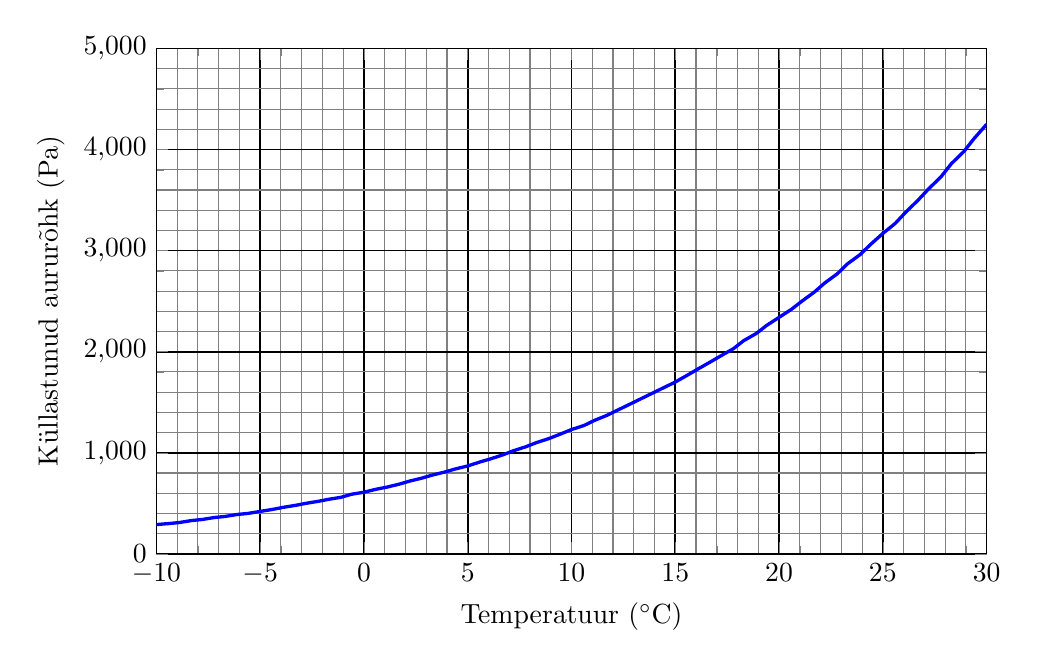
\begin{tikzpicture}
    \begin{axis}[
      xlabel={Temperatuur ($^\circ$C)},
      ylabel={Küllastunud aururõhk (Pa)},
      xmin=-10, xmax=30,
      ymin=0, ymax=5000,
      xtick={-10,-5,0,5,10,15,20,25,30},
      ytick={0,1000,2000,3000,4000,5000},
      minor tick num=4,
      grid=both,
      minor grid style={thin,gray},
      major grid style={semithick,black},
      width=\textwidth,
      height=8cm,
      ]

      \addplot[color=blue,very thick]
      coordinates {
        (-10.00,290.0)
        (-9.40,300.0)
        (-8.90,310.0)
        (-8.30,330.0)
        (-7.80,340.0)
        (-7.20,360.0)
        (-6.70,370.0)
        (-6.10,390.0)
        (-5.60,400.0)
        (-5.00,420.0)
        (-4.40,440.0)
        (-3.90,460.0)
        (-3.30,480.0)
        (-2.80,500.0)
        (-2.20,520.0)
        (-1.70,540.0)
        (-1.10,560.0)
        (-0.60,590.0)
        (0.00,610.0)
        (0.60,640.0)
        (1.10,660.0)
        (1.70,690.0)
        (2.20,720.0)
        (2.80,750.0)
        (3.30,780.0)
        (3.90,810.0)
        (4.40,840.0)
        (4.40,840.0)
        (5.00,870.0)
        (5.60,910.0)
        (6.10,940.0)
        (6.70,980.0)
        (7.20,1020.0)
        (7.80,1060.0)
        (8.30,1100.0)
        (8.90,1140.0)
        (9.40,1180.0)
        (10.00,1230.0)
        (10.60,1270.0)
        (11.10,1320.0)
        (11.70,1370.0)
        (12.20,1420.0)
        (12.80,1480.0)
        (13.30,1530.0)
        (13.90,1590.0)
        (14.40,1640.0)
        (15.00,1700.0)
        (15.60,1770.0)
        (16.10,1830.0)
        (16.70,1900.0)
        (17.20,1960.0)
        (17.80,2030.0)
        (18.30,2110.0)
        (18.90,2180.0)
        (19.40,2260.0)
        (20.00,2340.0)
        (20.60,2420.0)
        (21.10,2500.0)
        (21.70,2590.0)
        (22.20,2680.0)
        (22.80,2770.0)
        (23.30,2870.0)
        (23.90,2960.0)
        (24.40,3060.0)
        (25.00,3170.0)
        (25.60,3270.0)
        (26.10,3380.0)
        (26.70,3500.0)
        (27.20,3610.0)
        (27.80,3730.0)
        (28.30,3860.0)
        (28.90,3980.0)
        (29.40,4110.0)
        (30.00,4250.0)
      };
    \end{axis}
  \end{tikzpicture}
  \vspace{-3em}
\end{center}
\probend
\bigskip

% Ü93
\setAuthor{Jaan Kalda}
\setRound{lahtine}
\setYear{2024}
\setNumber{G 5}
\setDifficulty{5}
\setTopic{TODO}

\prob{Värske õhk}
Anu hoiab õhutusakna osaliselt lahti, parasjagu nii palju, et süsihappegaasi sisaldus toas ei oleks suurem, kui 1000 ppm. Lühend ppm tähendab ``osakest miljoni kohta'', st antud juhul ei tohi iga miljoni õhumolekuli kohta olla õhus rohkem, kui 1000 süsihappegaasi molekuli. Õueõhus on süsihappegaasi sisaldus 420 ppm ja temperatuur  $t_0=\SI{-10}{\celsius}$ ja õhurõhk $p=\SI{1e5}{\pascal}$. Toas on kolm inimest, kellest igaüks toodab $v=\SI{17}{\litre\per\hour}$  süsihappegaasi. Millise võimsusega on vaja tuba kütta, et hoida toatemperatuur $t_1=\SI{20}{\celsius}$ juures? Soojuskaudega läbi aknaklaaside, seinte jms mitte arvestada.
\probend
\bigskip

% Ü94
\setAuthor{Marten Rannut}
\setRound{piirkonnavoor}
\setYear{2024}
\setNumber{G 5}
\setDifficulty{5}
\setTopic{TODO}

\prob{Amoksitsilliin}
Juku läks tugeva kurguvaluga perearsti juurde, diagnoosiks osutus angiin ning Juku sai raviks $m= \SI{500}{\milli\gram}$ amoksitsilliinitabletid. Kui pika aja tagant on Jukul vaja üks tablett võtta? Juku kaalub $M= \SI{70}{\kilo\gram}$, ravimi minimaalne efektiivne kontsentratsioon kehakaalu kohta on $\SI{140}{\ug\per\kg}$. Amoksitsilliini poolestusaeg on $t= \SI{1.4}{\hour}$. \textit{Vihje:} Poolestusaja möödudes langeb aine kogus organismis poole võrra. Et ravim oleks efektiivne, peab selle kontsentratsioon kehas igal ajahetkel ületama minimaalset efektiivset kontsentratsiooni.
\probend
\bigskip

% Ü95
\setAuthor{Sandra Schumann}
\setRound{lõppvoor}
\setYear{2024}
\setNumber{G 5}
\setDifficulty{5}
\setTopic{TODO}

\prob{Joonlaud koridoris}
Seisad \SI{1}{\m} laiuses koridoris, mille mõlemas seinas on peegel. Peeglite vahel, parempoolsest peeglist \SI{30}{\cm} kaugusel asetseb vertikaalselt kitsas objekt. Sina oled koridoris, käes joonlaud, mida hoiad vertikaalselt enda ees. Märkad, et joonlaua \SI{10}{\cm} näib sulle sama pikk kui objekt ise, \SI{7.5}{\cm} sama pikk kui objekti peegeldus parempoolses peeglis ja \SI{3.75}{\cm} sama pikk kui objekti teine peegeldus parempoolses peeglis. Kui kaugel seisad peeglist?
\probend
\bigskip

% Ü96
\setAuthor{Kaarel Hänni}
\setRound{lahtine}
\setYear{2018}
\setNumber{G 6}
\setDifficulty{6}
\setTopic{TODO}

\prob{Magnetväljad}
Vaatleme prootoni liikumist x-y-tasandis. Vahemikus $0\leq x < \ell_1$ on magnetväli tugevusega $B$ z-telje positiivses suunas, vahemikus $\ell_1\leq x < \ell_1+\ell_2$ on magnetväli tugevusega $B$ z-telje negatiivses suunas. On teada, et $\ell_2 > \ell_1$. Ülejäänud tasandi osades magnetvälja pole. Alguses antakse prootonile mingi kiirus $\vec{v}$ tasandi vasakus pooles $x<0$. Milline on minimaalne kiirus $v=|\vec{v}|$, mille puhul saab valida sellise algse liikumissuuna, et prooton jõuab läbi kahe magnetväljaga vahemiku tasandi parempoolsesse osasse $x\geq \ell_1+\ell_2$? Prootoni laeng on $q$ ja mass on $m$.
\begin{centering}
	
	\begin{tikzpicture}
	{
		\tikzset{ % This was originally used to update the global tikz style, but I prefer it to be locally defined instead
			odot/.style={
				circle,
				inner sep=0pt,
				node contents={$\odot$},
				scale=2
			},
			otimes/.style={
				circle,
				inner sep=0pt,
				node contents={$\otimes$},
				scale=2
			},
			circ/.style={
				circle,
				draw,
				minimum size=3mm,
				inner sep=0
			},
			odot2/.style={
				circ,
				path picture={\fill circle[radius=1pt];}
			},
			otimes2/.style={
				circ,
				path picture={
					\draw (path picture bounding box.45) -- (path picture bounding box.225);
					\draw (path picture bounding box.135) -- (path picture bounding box.315);
				}
			}
		}
		\draw[->] (-4,0) -- (4,0) node[below] {x};
		\draw[->] (-2,-2) -- (-2,3) node[left] {y};
		\draw (0,-2) -- (0,3);
		\draw (3,-2) -- (3,3);
		\draw[->] (-3.5,1) -- (-2.2,0.4) node[midway, below left] {$\vec{v}$};
		
		\draw [decorate,decoration={brace,amplitude=10pt}]
		(-2,0) -- (0,0) node [above, black,midway, yshift=7] {$\ell_1$}; 
		
		\draw [decorate,decoration={brace,amplitude=10pt}]
		(0,0) -- (3,0) node [above, black,midway, yshift=7] {$\ell_2$};
		
		\node [odot2] at (-1,2) {};
		\node [otimes2] at (1.5,2) {};
		\node at (-0.65,2) {$\vec{B}$};
		\node at (1.85,2) {$\vec{B}$};
	}
	\end{tikzpicture}
\end{centering}
\probend
\bigskip

% Ü97
\setAuthor{Ardi Loot}
\setRound{lahtine}
\setYear{2019}
\setNumber{G 6}
\setDifficulty{6}
\setTopic{TODO}

\prob{Led}
\begin{wrapfigure}[7]{r}{0.5\textwidth}
	\vspace{-24pt}
	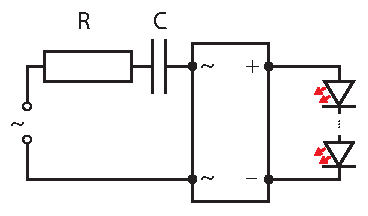
\includegraphics[width=0.5\textwidth]{2019-lahg-06-yl.pdf}
\end{wrapfigure}

LED-lamp koosneb $N=10$-st valgusdioodist (nimipinge $U_{D}=\SI{3.0}{V}$ ja -vool $I_{D}=\SI{100}{mA}$), mida toidetakse vahelduvvooluga (pinge maksimumväärtus $U=\SI{320}{V}$ ja sagedus $f=\SI{50}{Hz}$) läbi takisti ($R=\SI{400}{\ohm}$), kondensaatori ja alaldi (lugeda ideaalseks). Kui suur peab olema kondensaatori mahtuvus $C,$ et valgusdioodid põleksid võimalikult heledalt, kuid ei põleks läbi? Märkus: Takisti ja kondensaatori näivtakistus on $Z=\sqrt{R^{2}+X_{C}^{2}}$, kus $X_{C}=1/\left(2\pi fC\right)$ ning võib eeldada sinusoidaalset voolu ja pinget aladi ees.
\probend
\bigskip

% Ü98
\setAuthor{}
\setRound{piirkonnavoor}
\setYear{2019}
\setNumber{G 6}
\setDifficulty{6}
\setTopic{TODO}

\prob{Kondensaator}
\begin{wrapfigure}[6]{r}{0.30\textwidth}
\vspace{-45pt}
	\begin{center}
		\includegraphics[width = 0.30\textwidth]{2019-v2g-06-yl.pdf}
	\end{center}
\end{wrapfigure}


Kondensaatorit laetakse kõrvaloleva skeemi järgi alalisvooluallikast pingega $U=\SI{12}{\V}$. Skeemis olevate takistite takistused on vastavalt $R_1=\SI{1}{\kilo\ohm}$, $R_2=\SI{2}{\kilo\ohm}$ ning $R_3=\SI{3}{\kilo\ohm}$. Leida maksimaalne pinge, milleni saame kondensaatori niimoodi laadida. 
\vspace{10pt}
\probend
\bigskip

% Ü99
\setAuthor{}
\setRound{lõppvoor}
\setYear{2019}
\setNumber{G 6}
\setDifficulty{6}
\setTopic{TODO}

\prob{Lõks}
Kuulike massiga $m$ ja laenguga $q$ sisenes läbi väikse augu silindrisse, mida täidab teljesihiline homogeenne magnetväli induktsiooniga $B$. Sisenemishetkel oli kuulikese kiirus radiaalsihiline. Kuulike väljus silindrist sama augu kaudu peale kahte absoluutselt elastset põrget silindri seintega. Kui kaua viibis kuulike silindris? 
\vspace{-5pt}
\probend
\bigskip

% Ü100
\setAuthor{Taavet Kalda}
\setRound{lahtine}
\setYear{2020}
\setNumber{G 6}
\setDifficulty{6}
\setTopic{TODO}

\prob{Kondensaatorid}
\begin{wrapfigure}[8]{r}{0.3\linewidth}
		\vspace{-5pt}
		\includegraphics[width=\linewidth]{2020-lahg-06-yl.pdf}
	\end{wrapfigure}
	Pingeallikas pingega $\mathcal E$ on ühendatud kolme kondensaatoriga mahtuvustega $C_1$, $C_2$ ja $C_3$. Alguses hoitakse lüliti pikalt kinnises olekus. Mitu korda muutub punktide $A$ ja $B$ vaheline pinge peale lüliti avamist ja pika aja möödumist?
\probend
\bigskip

% Ü101
\setAuthor{}
\setRound{piirkonnavoor}
\setYear{2020}
\setNumber{G 6}
\setDifficulty{6}
\setTopic{TODO}

\prob{Kell}
Seinakellal on minuti ja tunniosuti, mis kaaluvad vastavalt
$m_1=\SI{5}{\gram}$ ja $m_2=\SI{25}{\gram}$, mille pikkused on vastavalt
$L_1=\SI{15}{\centi\meter}$ ja $L_2=\SI{10}{\centi\meter}$ ning mille otspunktid
on kinnitatud kella keskpunkti. Kella vooluallikas on tühjenemas ning täpselt kell kuus annab see maksimaalselt voolu $I=\SI{1}{\milli\ampere}$ pingel
$V=\SI{5}{\volt}$. Elektrienergiast jõuab osutiteni mehaaniline energia
kasuteguriga $\eta=0.3$. Leia minuti täpsusega aeg, mil kell jääb seisma.
\probend
\bigskip

% Ü102
\setAuthor{}
\setRound{lõppvoor}
\setYear{2020}
\setNumber{G 6}
\setDifficulty{6}
\setTopic{TODO}

\prob{Palliviskenõlv}
Oleg viskab jalgpalliväljaku otsajoone tagant väljakule palli. Selgub, et sealt
jaksab ta visata maksimaalselt väljaku keskjooneni, mis asub kaugusel $L$. Ta
tahab ehitada otsajoone taha sellise nõlva, mille igast punktist jaksaks ta visata
maksimaalselt väljaku keskjooneni. Milline peaks olema selle nõlva kõrgusprofiil?

Võib eeldada, et maksimaalne kiirus, millega Oleg suudab palli visata, ei sõltu
viskamissuunast. Õhutakistust võib ignoreerida. Vastuse võib anda kujul $y=f(x)$
või $x=g(y)$.
\probend
\bigskip

% Ü103
\setAuthor{Jaan Kalda}
\setRound{lahtine}
\setYear{2021}
\setNumber{G 6}
\setDifficulty{6}
\setTopic{TODO}

\prob{Kaugusvise}
Mis nurga all tuleb ühtlase kaldega pinnal (kaldenurk $\alpha$) visata, et pall lendaks fikseeritud algkiiruse juures võimalikult kaugele?
\probend
\bigskip

% Ü104
\setAuthor{Jarl Patrick Paide}
\setRound{piirkonnavoor}
\setYear{2021}
\setNumber{G 6}
\setDifficulty{6}
\setTopic{TODO}

\prob{Jalgrattur}
Samal ajal, kui jalgrattur sõidab mööda kindlat teelõiku, alustab auto juhuslikul ajahetkel juhuslikust kohast sellel teelõigul sõitu. Auto sõidab jalgratturiga samas suunas, kuid kaks korda kiiremini, ning mõlemad sõidavad teelõigu lõpuni. Mis on tõenäosus, et auto sõidab jalgratturist mööda?
\probend
\bigskip

% Ü105
\setAuthor{Krister Kasemaa}
\setRound{lõppvoor}
\setYear{2021}
\setNumber{G 6}
\setDifficulty{6}
\setTopic{TODO}

\prob{Keha keral}
Kerakujulisele, ühtlase massijaotusega planeedile, raadiusega $R$, massiga $M$ ja pöörlemisperioodiga $T$ asetatakse väikese massiga keha $m$. Gravitatsioonikonstant on G.\\
\osa Leia väikese keha kaal funktsioonina laiuskraadist $\theta$.\\
\osa Leia hõõrdeteguri $\mu$ väärtuste vahemik funktsioonina laiuskraadist $\theta$, mille puhul püsib väike keha planeedi peal staatilisena. \par
\emph{Märkus:} laiuskraadi $\theta$ mõõdetakse ekvaatorilt.
\probend
\bigskip

% Ü106
\setAuthor{Jaan Kalda}
\setRound{lahtine}
\setYear{2022}
\setNumber{G 6}
\setDifficulty{6}
\setTopic{TODO}

\prob{Saun}
Subjektiivset palavusetunnet kuumas õhus kirjeldab väga hästi see, kui palju erineb kastepunkt keha temperatuurist. Kastepunkt on temperatuur, mille juures antud õhust hakkab vesi välja kondenseeruma (eeldusel, et rõhk püsib võrdne atmosfäärirõhuga). Olgu leiliruumi õhutemperatuur $T_l=\SI{100}{\celsius}$, saunaõhu kastepunkt $T_k=\SI{10}{\celsius}$ ja leiliruumi ruumala $V=\SI{10}{m^3}$. Mitme kraadini kerkib kastepunkt, kui leiliks vistakase $m=\SI{200}g$ vett? Universaalne gaasikonstant $R=\SI{8.31}{\joule\per\kelvin\per\mole}$; vee molaarmass $\mu=\SI{18}{\gram \per \mole}$.
\begin{center}
    \includegraphics[width=\textwidth]{2022-lahg-06-yl.pdf}
\end{center}
\probend
\bigskip

% Ü107
\setAuthor{Päivo Simson}
\setRound{piirkonnavoor}
\setYear{2022}
\setNumber{G 6}
\setDifficulty{6}
\setTopic{TODO}

\prob{Doomino}
\begin{wrapfigure}{r}{2.8cm}
  \vspace{-2em}
  \begin{center}
    \includegraphics[width=2.8cm]{2022-v2g-06-yl.pdf}
  \end{center}
  \vspace{-2em}
\end{wrapfigure}
Väike kuulike liigub horisontaalselt kiirusega $u$ joonisel näidatud suunas ja kukub alla kõrguselt $H$. Alumisel tasapinnal on doominoklots kõrgusega $h$, mis kukub ümber, kui kuulike sellele pihta läheb. Klotsi kaugus astmest on $d$. Leidke minimaalne algkiirus $u$, mille korral kuulike teeb ühe põrke ja lendab seejärel klotsist üle. Eeldage, et õhutakistus ja hõõrdejõud puuduvad ning põrge on absoluutselt elastne. Klotsi paksusega ja kuuli mõõtmetega ei pea arvestama. Raskuskiirendus on $g$.
\probend
\bigskip

% Ü108
\setAuthor{Jaan Kalda}
\setRound{lõppvoor}
\setYear{2022}
\setNumber{G 6}
\setDifficulty{6}
\setTopic{TODO}

\prob{Õhupüss}
Õhupüssis kasutatakse rõhu $p_1=\SI{34}{MPa}$ all olevat lämmastikku kuuli kiirendamiseks. Milline on püssirauda jääva lämmastiku temperatuur vahetult peale lasku? Enne lasku oli surulämmastik toatemperatuuril $t_0=\SI{20}\celsius$; õhurõhk $p_0=\SI{100}{kPa}$. Lämmastiku molaarne soojusmahtuvus konstantsel ruumalal on $c_V=\frac 52R$ ja keemistemperatuur $T_k=\SI{-196}\celsius$. \\
\textit{Vihje:} Helikiirusest aeglasemates protsessides gaasiga, kus ei toimu soojusvahetust, kehtib nn adiabaadiseadus $pV^\gamma=const$, kus lämmastiku jaoks on astmenäitaja $\gamma=7/5$.
\probend
\bigskip

% Ü109
\setAuthor{Marten Rannut}
\setRound{lahtine}
\setYear{2023}
\setNumber{G 6}
\setDifficulty{6}
\setTopic{TODO}

\prob{Võimas mootor}
K20A on 4-taktiline, 4-silindriline, \SI{2,0}{\liter} mootor (iga silindri maht on \SI{0,5}{\liter}), mis saavutab oma tippvõimsuse $f= \SI{8000}{\per\minute}$ (pööret/min) juures. Üks takt kestab pool pööret, taktid on: sisselasketakt, survetakt, töötakt ja väljalasketakt.
Temperatuuril $T_1=\SI{20}\celsius$ on õhu tihedus $\rho=\SI{1.2}{\kg\per\m\cubed}$; kui välistemperatuur on $T_1$, siis on sissevõtutakti lõpus silindris oleva õhu temperatuur $T_2=\SI{60}\celsius$.  Sissevõtutakti lõpus kolbi pritsitud bensiini ruumalaga mitte arvestada. Leidke sellise mootori tippvõimsus.
Bensiini energiatihedus on $\epsilon = \SI{46}{\mega\joule\per\kilogram}$, ideaalne kulunud õhu ja bensiini suhe on $\gamma = \frac{\SI{14,7}{\gram}}{\SI{1}{\gram}}$. Võib eeldada, et toimub täielik põlemine. Mootori efektiivsus on $\eta=37\%$.
\probend
\bigskip

% Ü110
\setAuthor{Erkki Tempel}
\setRound{piirkonnavoor}
\setYear{2023}
\setNumber{G 6}
\setDifficulty{6}
\setTopic{TODO}

\prob{Klaasplaat}
\begin{wrapfigure}{r}{0.3\textwidth}
  \vspace{-2em}
  \begin{center}
    \includegraphics[width=1\linewidth]{2023-v2g-06-yl.pdf}
    %\caption{}
  \end{center}
  \vspace{-2em}
\end{wrapfigure}

Leidke, kui palju nihkub valguskiir kõrvale esialgse sihi suhtes pärast klaasplaadi läbimist. Kiire langemisnurk on $\alpha$, klaasi murdumisnäitaja on $n$ ning klaasplaadi paksus on $d$. Täispunktide saamiseks palume vastuses mitte kasutada trigonomeetrilisi pöördfunktsioone (nt $\arcsin$, $\arccos$).
\probend
\bigskip

% Ü111
\setAuthor{Martne Rannut}
\setRound{lõppvoor}
\setYear{2023}
\setNumber{G 6}
\setDifficulty{6}
\setTopic{TODO}

\prob{Nõel vees}
Nõel massiga $m=\SI{0.5}{\g}$ ning pikkusega $l=\SI{6}{\cm}$ asetatakse aeglaselt vee pinnale. Millise nurga alla on veepind nõela juures horisontaalpinna suhtes paindunud? Vee pindpinevustegur $\sigma=\SI{72.8}{\mN\per\m}$ ja raskuskiirendus $g=\SI{9.81}{\m\per\s\squared}$. Üleslükkejõuga võib mitte arvestada.
\probend
\bigskip

% Ü112
\setAuthor{Jaan Kalda}
\setRound{lahtine}
\setYear{2024}
\setNumber{G 6}
\setDifficulty{6}
\setTopic{TODO}

\prob{Vari}
\begin{wrapfigure}{r}{0.4\textwidth}
\vspace{-0.8cm}
  \begin{center}
    \includegraphics[width=1\linewidth]{2024-lahg-06-yl.pdf}
  \end{center}
  \vspace{-0.9cm}
\end{wrapfigure}

Joonisel (suurem koopia lisalehel) on näidatud ülaltvaates horisontaalsel laual lebav kera ja selle vari, mille heidab lauale punktvalgusallikas. Mitme kera raadiuse kaugusel kera keskpunktist asub see punktvalgusallikas? Võite teha joonisel lisakonstruktsioone ja mõõtmisi.
\probend
\bigskip

% Ü113
\setAuthor{Päivo Simson}
\setRound{piirkonnavoor}
\setYear{2024}
\setNumber{G 6}
\setDifficulty{6}
\setTopic{TODO}

\prob{Mitteelastne nöör}
\begin{wrapfigure}{r}{0.33\textwidth}
\vspace{-20pt}
  \begin{center}
    \includegraphics[width=1\linewidth]{2024-v2g-06-yl.pdf}
  \end{center}
  \vspace{-15pt}
\end{wrapfigure}

Väike kuulike on kinnitatud mitteelastse nööri külge ja seda hoitakse esialgu punktis $K$. Nööri pikkus on $l$ ja selle teine ots on kinnitatud punkti $P$. Punktid $K$ ja $P$ asuvad samal kõrgusel $h=l$ ja nendevaheline kaugus on $a$ ($0<a<l$). Nüüd lastakse kuulike ilma algkiiruseta vabaks ja see hakkab gravitatsiooni mõjul liikuma. Leidke maksimaalne kõrgus, mille kuulike saavutab $h=0$ suhtes edaspidise liikumise käigus (pärast täielikku kukkumist). Tehke kuuli trajektoori joonis. Nööri mass on võrreldes kuuli massiga tühine ning takistusjõududega võib mitte arvestada. Nööri mitteelastsus tähendab seda, et põrke hetkel summutab nöör kogu palli nöörisihilise impulsi.
\probend
\bigskip

% Ü114
\setAuthor{Uku Andreas Reigo}
\setRound{lõppvoor}
\setYear{2024}
\setNumber{G 6}
\setDifficulty{6}
\setTopic{TODO}

\prob{Jahtumine}
Sofial on kaks ühesugust koonusekujulist kaaneta termost, mis on osaliselt täidetud võrdse koguse vedelikuga temperatuuril $T=\SI{40}{\celsius}$. Koonusekujulised termosed on asetatud nii, et vedelikupind on põhjaga paralleelne ja koonuse tipp on allpool. Sofia lisab ühte termosesse juurde sama koguse soojemat vedelikku temperatuuril $T_\text{lisa} = \SI{88}{\celsius}$, soojuslik tasakaal saabub hetkeliselt. Seejärel mõõdab Sofia otsekohe vedelike jahtumiskiirust ning leiab, et soojema vedeliku jahtumise kiirus on $k=\num{1.62}$ korda suurem jahedama vedeliku jahtumise kiirusest. Jahtumisvõimsus on võrdeline jahutatava pindala ja temperatuuride vahega. Leidke õhutemperatuur $T_\text{õhk}$. Eeldage, et vedeliku ja termose vahel soojusvahetust ei toimu ning et vedeliku tihedus ei sõltu temperatuurist.

\textit{Vihje}: koonuse ruumala $V=\frac{1}{3}S_p H$, kus $S_p$ on koonuse põhja pindala ning $H$ selle kõrgus.
\probend
\bigskip

% Ü115
\setAuthor{Krister Kasemaa}
\setRound{lahtine}
\setYear{2018}
\setNumber{G 7}
\setDifficulty{7}
\setTopic{TODO}

\prob{Kauss veega}
Kaalul olevasse kaussi hakatakse ühtlaselt pudelist kõrgusel $h$ vett valama. Vee valamine lõpetatakse hetkel, mil kaalu näit on $m$. Mis on kaalu lugem $M$ peale stabiliserumist? Kas see on esialgsest näidust suurem, väiksem või võrdne? Õhutakistusega mitte arvestada.
\probend
\bigskip

% Ü116
\setAuthor{Jaan Kalda}
\setRound{lahtine}
\setYear{2019}
\setNumber{G 7}
\setDifficulty{7}
\setTopic{TODO}

\prob{Niit relssidel}
\begin{wrapfigure}[7]{r}{0.3\textwidth}
	\vspace{-13pt}
	\includegraphics[width=0.3\textwidth]{2019-lahg-07-yl.pdf}
\end{wrapfigure}

Niit kogupikkusega $L$ on kinnitatud kahest üksteisega ristuvast lõigust koosneva relsi külge nii, nagu näidatud joonisel: üks ots on fikseeritud jäigalt vertikaalse relsiosa külge kaugusele $h$ relsi nurgast, alumine ots tillukese rõnga abil horisontaalse relsi külge. Niit on tõmmatud läbi teise tillukese rõnga, mis saab libiseda mööda vertikaalset relssi. Alumist rõngast liigutatakse konstantse kiirusega $v$. Leida teise rõnga kiirus ja kiirendus hetkel, mil nöör moodustab nurga $\alpha$ horisontaalsihiga.
\probend
\bigskip

% Ü117
\setAuthor{}
\setRound{piirkonnavoor}
\setYear{2019}
\setNumber{G 7}
\setDifficulty{7}
\setTopic{TODO}

\prob{Lennurada}
Lennuk vajab õhkutõusmiseks vajaliku üleslükkejõu saavutamiseks merepinna kõrgusel vähemalt $L=\SI{2}{km}$ pikkust hoorada. Kui pikka hoorada vajaks sama lennuk maailma kõrgeimal tsiviillennuväljal, mis asub merepinnast $\SI{4}{km}$ kõrgusel? Õhu tihedus merepinnal $\rho_1 = \SI{1,23}{kg/m^3}$ ning $\SI{4}{km}$ kõrgusel $\rho_2 = \SI{0,82 }{kg/m^3}$. Lennuki tiibade poolt tekitatav üleslükkejõud on võrdeline õhu tiheduse ning lennuki kiiruse ruuduga. Eeldada, et ilm on mõlemal juhul tuulevaikne ning lennuki kiirendus on kogu hoovõtu jooksul konstantne.
\probend
\bigskip

% Ü118
\setAuthor{}
\setRound{lõppvoor}
\setYear{2019}
\setNumber{G 7}
\setDifficulty{7}
\setTopic{TODO}

\prob{3 ruutu}
\begin{wrapfigure}[4]{r}{0.45\textwidth}
  \vspace{-15pt}
  \begin{center}
  \includegraphics[scale=0.65]{2019-v3g-07-yl.pdf}
  \end{center}
  \vspace{-20pt}
\end{wrapfigure}



Toodud skeemis on kõigi takistite takistus kolm oomi, patarei pinge on 48 volti. Leidke ampermeetrite näidud. 
\vspace{25pt}
\probend
\bigskip

% Ü119
\setAuthor{Krister Kasemaa}
\setRound{lahtine}
\setYear{2020}
\setNumber{G 7}
\setDifficulty{7}
\setTopic{TODO}

\prob{Poolsilinder basseinis}
\
	Basseinis laiusega $l$ takistab vedeliku ühelt poolt teisele poole voolamist poolsilinder massiga $m$ ja raadiusega $r$ (ja seega pikkusega $l$), kusjuures telg, piki mida silinder on poolitatud, on vastu basseini põhja. Hõõrdetegur poolisilindri ja basseini põhja vahel on $\mu$, vedeliku tihedus basseinis $\rho$, ja raskuskiirendus on $g$. Basseini üks pool on täidetud veega poolsilindri ülemise ääreni, kõrguseni $r$. Küsimusele vastates eeldage, et hõõrdumine poolsilindri külgmiste poolringide ja seina vahel on tühiselt väike. Mis peaks olema hõõrdeteguri $\mu$ vähim väärtus $\mu_0$, et poolislindri vabastades ei hakkaks see liikuma?
\probend
\bigskip

% Ü120
\setAuthor{}
\setRound{piirkonnavoor}
\setYear{2020}
\setNumber{G 7}
\setDifficulty{7}
\setTopic{TODO}

\prob{Jälle sauna!}
Sauna leiliruumis on õhu temperatuur $t_0=\SI{80}\celsius$ ja leiliruumi ruumala $V=\SI{10}{m^3}$. Kerisele visati $m=\SI{200}g$ vett, mis paari sekundi jooksul kõik ära aurustus. Kui palju muutus õhu temperatuur leiliruumis? Eeldada, et tekkinud aur segunes täielikult leiliruumi õhuga ja rõhk leiliruumis püsis võrdne välise õhurõhuga tänu õhu liikimisele läbi uksealuse pilu. Õhurõhk $p_0=\SI{1e5}{Pa}$, vee molaarmass  $\mu_w=\SI{18}{g/mol}$, ühe mooli õhu soojusmahtuvus konstantsel ruumalal $c_a=\frac 53 R$ ja ühe mooli veeauru soojusmahtuvus konstantsel ruumalal $c_w=2R$.
\probend
\bigskip

% Ü121
\setAuthor{}
\setRound{lõppvoor}
\setYear{2020}
\setNumber{G 7}
\setDifficulty{7}
\setTopic{TODO}

\prob{Pulgad}
\begin{wrapfigure}{r}{0.35\textwidth}
  \vspace{-8pt}
  \begin{center}
  \includegraphics[scale=0.9]{2020-v3g-07-yl.pdf}
  \end{center}
  \vspace{-25pt}
\end{wrapfigure}
Kaks pulka pikkusega $L$ on otsapidi kinnitatud hõõrdevaba kinnitusega.
Hõõrdevabal horisontaalsel laual on silinder raadiusega $R$ ja massiga $m$.
Joonisel on kujutatud silinder ja pulgad pealtvaates. Eeldame, et pulki hoitakse
alati horisontaalselt nagu joonisel, nendega haaratakse kinni silindri keskelt,
pulkade otsad on täpselt silindri puutepunktides ning pulkade mass on tühine.
Samuti eeldame, et silindri massikese on puutepunkte ühendava lõigu keskpunktis.\\
\osa Leidke minimaalne hõõrdetegur $\mu_{\min}$ pulkade ja silindri vahel,
et silindrist pulkade abil kinni haarates see pulkade vahelt ära ei libiseks.\\
\osa Olgu hõõrdetegur pulkade ja silindri vahel $\mu > \mu_{\min}$. Leidke
minimaalne vajalik jõumoment $\tau_{\min}$, mida tuleb pulkadele avaldada, et
silindrist pulkade abil kinni haarates oleks võimalik silinder laualt üles
tõsta. Maa raskuskiirendus on $g$.
\probend
\bigskip

% Ü122
\setAuthor{Jaan Kalda}
\setRound{lahtine}
\setYear{2021}
\setNumber{G 7}
\setDifficulty{7}
\setTopic{TODO}

\prob{Hantel}
Kaks pisikest kera, kumbki massiga $m$, on ühendatud üksteise külge kerge jäiga varda abil, mille pikkus on $l$; nimetagem seda süsteemi edaspidi hantliks. Üks kera kannab laengut $q$, kuid teine on ilma laenguta. Alghetkel on hantel horisontaalne ning liikumatu ja asub vertikaalses elektriväljas tugevusega $E$; raskusväli puudub. Milline on hantli telje pöörlemise maksimaalne nurkkiirus $\omega$ edasise liikumise käigus?
\probend
\bigskip

% Ü123
\setAuthor{Kaur Aare Saar}
\setRound{piirkonnavoor}
\setYear{2021}
\setNumber{G 7}
\setDifficulty{7}
\setTopic{TODO}

\prob{Rippuv laeng}
Punktlaeng $q_1$ ripub lakke kinnitatud nööri otsas, mille pikkus on $L$. Teine samamärgiline punktlaeng $q_2$ on nöörist sõltumatult fikseeritud täpselt nööri kinnituskoha alla kaugusele $2h$ laest. Leidke milline peab olema esimese punktlaengu mass, et selle kaugus laest oleks $h$.
\probend
\bigskip

% Ü124
\setAuthor{Jaan Kalda}
\setRound{lõppvoor}
\setYear{2021}
\setNumber{G 7}
\setDifficulty{7}
\setTopic{TODO}

\prob{Kolmnurk}
Kolm ühesuguse massiga $m$ osakest paigutatakse punktidesse $A$, $B$ ning $C$. Osakeste mõõtmed on palju väiksemad kolmnurga $ABC$ küljepikkustest $a=|BC|$, $b=|CA|$ ja $c=|AB|$. Osake punktis $A$ kannab laengut $q_A$, osake punktis $B$ --- laengut $q_B$ ja osake punktis $C$ --- laengut $q_C$. Osakesed vabastatakse ning need hakkavad paigalseisust liikuma elektrostaatilise vastasmõju tõttu.\\
\osa Millised peaksid olema laengute suhted, et kõigi osakeste trajektoorid oleksid sirgjooned?\\
\osa Kas sirgjooneline liikumine on võimalik suvalise kolmnurga $ABC$ puhul?
\probend
\bigskip

% Ü125
\setAuthor{Jaan Kalda}
\setRound{lahtine}
\setYear{2022}
\setNumber{G 7}
\setDifficulty{7}
\setTopic{TODO}

\prob{Elektron ja kondensaator}
Plaatkondensaatori plaadid on ruudukujulised küljepikkusega $b$ ja plaatide vahekaugus $d$ on hulga väiksem kui $b$; plaatide vahele on rakendatud pinge $U$. Millist minimaalset algkiirust $v$ peab omama elektron massiga $m$ ja laenguga $e$, et see suudaks läbida plaatide vahelise ruumi ilma vastu plaate põrkamata? Elektron peab väljuma plaatidevahelisest ruumist sisenemispunkti suhtes vastasküljelt.
\probend
\bigskip

% Ü126
\setAuthor{Taavet Kalda}
\setRound{piirkonnavoor}
\setYear{2022}
\setNumber{G 7}
\setDifficulty{7}
\setTopic{TODO}

\prob{Plastiliin}
Laua peal asub vedrudel toetuv tasakaaluasendis olev plaat. Vedrude summaarne jäikustegur on $k$. Plaadi pinnale kõrguselt $h$ kukutatakse ideaalselt plastne plastiliinitükk massiga $m$. Mõne aja pärast kukutatakse samalt kõrguselt teine identse massiga plastiliinitükk nii, et plastiliinitükk langeb plaadi pinnale hetkel, mil plaat on liikumas üles ja esialgse tasakaaluasendiga võrreldes samal kõrgusel. Mis on plaadi edasise trajektoori kõige madalama asendi kõrguse ja esialgse tasakaaluasendi kõrguse vahe? Plaadi mass on plastiliini massiga võrreldes tühine, plastiliin kleepub pärast põrget plaadi külge ning õhutakistust ja vedrude hõõrdetakistust võib ignoreerida. Raskuskiirendus on $g$.
\probend
\bigskip

% Ü127
\setAuthor{Oleg Košik}
\setRound{lõppvoor}
\setYear{2022}
\setNumber{G 7}
\setDifficulty{7}
\setTopic{TODO}

\prob{Veeuputus}
Tänava kanalisatsioon on ehitatud selliselt, et vihmasaju korral koguneb vihmavesi kõigepealt tänava all kulgevasse kraavi, kust omakorda juhitakse vesi ära sadeveetorustiku kaudu. Sadeveetorustiku ummistuse tõttu suudab see aga tagada sadevee äravoolu ainult 50\% võimsusel maksimaalsest võimalikust. Ükskord paduvihma ajal juba 6 minutit peale vihma algust sai kraav täis ning vesi tungis tänavale. Graafikul (pöördel) on toodud sademete koguhulga $h$ sõltuvus ajast $t$ alates paduvihma algusest. \\
Peale paduvihma lõppemist tehtud arvutused näitasid, et isegi juhul, kui sadeveetorustik poleks ummistunud, poleks see uputusest päästnud ning kraav oleks täitunud 9 minutit peale vihma algust.\\
Milline pidanuks olema töökorras torustiku äravoolu minimaalne võime (liitrit minutis $\SI{1} {m^2}$ pinna kohta), et uputust ei oleks tekkinud?
\probend
\bigskip

% Ü128
\setAuthor{Jaan Kalda}
\setRound{lahtine}
\setYear{2023}
\setNumber{G 7}
\setDifficulty{7}
\setTopic{TODO}

\prob{Soojuspump}
Hilissügisel maamajja minnes on nii õues kui toas $T_0=\SI {2}{\celsius}$ sooja. Kui soojuspump sisse lülitada, kulub toas keskmise temperatuur  tõusmiseks $T_1=\SI {4}{\celsius}$-ni $t_0=\SI{30}{\min}$. Kui soojuspump jääkski pidevalt töötama, tõuseks temperatuur toas lõpuks $T_f=\SI {42}{\celsius}$-ni. Paraja soojuse tagamiseks lülitab soojuspumpa sisse ehitatud termorelee pumba välja, kui toatemperatuur tõuseb üle $T_3=\SI{23}\celsius$ ning uuesti sisse tagasi, kui temperatuur langeb alla $T_2=\SI{22}{\celsius}$. Kui pikk on ajavahemik kahe järjestikuse sisse lülitumise vahel? Eeldage, et soojuspumba kütmisvõimsus on kogu aeg üks ja sama. Lahendamisel võib teha täiendavaid mõistlikke lähendusi.\\ \emph{Märkus:} Võite eeldada, et soojuskadu on võrdeline temperatuuride vahega.
\probend
\bigskip

% Ü129
\setAuthor{Päivo Simson}
\setRound{piirkonnavoor}
\setYear{2023}
\setNumber{G 7}
\setDifficulty{7}
\setTopic{TODO}

\prob{Voltmeeter}
\begin{wrapfigure}{r}{0.35\textwidth}
  \begin{center}
    \includegraphics[width=1\linewidth]{2023-v2g-07-yl.pdf}
  \end{center}
  \vspace{-2em}
\end{wrapfigure}

Kolm tundmatut takistit on ühendatud jadamisi ja neile on rakendatud pinge $U=\SI{126}{\volt}$. Tundmatu sisetakistusega voltmeetriga mõõdetakse pingeid joonisel näidatud punktide vahel. Tulemuseks on näidud $V_{AB}=V_{CD}=\SI{28}{\volt}$ ja $V_{AC}=\SI{84}{\volt}$. Millist pinget näitab voltmeeter, kui selle klemmid ühendada punktidega B ja C?
\probend
\bigskip

% Ü130
\setAuthor{Eero Vaher}
\setRound{lõppvoor}
\setYear{2023}
\setNumber{G 7}
\setDifficulty{7}
\setTopic{TODO}

\prob{Tehiskaaslane}
Tehiskaaslane tiirleb ümber planeedi ringorbiidil raadiusega $r=\SI{55199}{\km}$ kiirusega $v=\SI{2.4}{\km\per\s}$. Tehiskaaslasele on lühikese aja jooksul võimalik anda kiiruse muut $\Delta v=\SI{0.7}{\km\per\s}$.
\\a) Mis oleks tehiskaaslase suurim kaugus planeedi keskmest $R_1$, kui tehiskaaslasele antaks kiirendus selle liikumissuunas?
\\b) Mis oleks suurim kaugus $R_2$, kui kiirenduse suund oleks planeedist eemale?
\probend
\bigskip

% Ü131
\setAuthor{Jarl Patrick Paide}
\setRound{lahtine}
\setYear{2024}
\setNumber{G 7}
\setDifficulty{7}
\setTopic{TODO}

\prob{Äikesetorm}
Helena mõõtis äikesetormi ajal Maa magnetvälja väga täpse elektroonilise magnetomeetriga. Ta hakkas muretsema äikesetormi mõjudest mõõtmistele ja otsustas seda uurida. Äikese sähvatusest kuni heli saabumiseni läks aega $t = \SI{10}{\s}$. Ta uuris välja, et tavalise äikselöögi voolutugevus on $I = \SI{30000}{\ampere}$, õhu magneetiline läbitavus on $\mu = \SI{1.26e-6}{\tesla\metre\per\ampere}$ ja heli kiirus õhus on $v_{õ} = \SI{340}{\m\per\s}$. Leia mitu kraadi maksimaalselt muutub mõõteriista poolt mõõdetud põhja suund löögi hetkel. Tavakeskkonnas magneomeeter mõõdab Maa magnetvälja tugevuseks $B = \SI{50}{\micro \tesla}$ ning magnetväli moodustab vertikaalse sihiga nurga $\alpha = 17^{\circ}$. \\
\textit{Vihje:} Sirge juhe voolutugevusega $I$ tekitab endast kaugusele $r$ magnetvälja tugevusega $B = \frac{\mu I}{2\pi r}$. Tekkinud magnetvälja suund on risti juhtmega ja tangensiaalne vastavalt kruvireeglile.
\probend
\bigskip

% Ü132
\setAuthor{Jaan Kalda}
\setRound{piirkonnavoor}
\setYear{2024}
\setNumber{G 7}
\setDifficulty{7}
\setTopic{TODO}

\prob{Palgid vees}
\begin{wrapfigure}{r}{0.3\textwidth}
  \vspace{-25pt}
  \begin{center}
  \includegraphics[scale=0.3]{2024-v2g-07-yl.pdf}
  \vspace{-20pt}
  \end{center}
\end{wrapfigure}

Kaks palki on kinnitatud üksteise külge nööri abil, mis läheb üle basseini põhja kinnitatud ploki nii nagu näidatud joonisel. Nöör on tõmmanud ühe palgi üleni vee alla sel ajal kui teine ujub vee pinnal. Mõlema palgi tihedus on $\rho=\SI {600}{\kg \per\m\cubed}$, vee tihedus $\rho_v=\SI{1000}{\kg\per\m\cubed}$, väiksema palgi ruumala on $V=\SI{30}\litre$ ja risttahuka kujulise basseini põhja pindala  $S=\SI{1}{m\squared}$. Kui palju muutub veetaseme kõrgus basseinis, kui palke ühendav nöör katki lõigata?
\probend
\bigskip

% Ü133
\setAuthor{Jaan Kalda}
\setRound{lõppvoor}
\setYear{2024}
\setNumber{G 7}
\setDifficulty{7}
\setTopic{TODO}

\prob{Romb}
\begin{wrapfigure}[9]{r}{0.1\textwidth}
  \vspace*{-0mm}
  \includegraphics[width = 0.1\textwidth]{2024-v3g-07-yl.pdf}
\end{wrapfigure}
Laest ripub rombikujuline liigendiga konstruktsioon, mis on valmistatud massita varrastest pikkusega $l$, vt joonis. Silinder massiga $m$ pannakse rombi sisse. Selle tulemusel võtab romb tasakaaluasendi, kus rombi tipunurk on $2\alpha$. Hõõrdumine silindri ja varda vahel on tühiselt väike. Leidke silindri raadius.
\probend
\bigskip

% Ü134
\setAuthor{Jaan Kalda}
\setRound{lahtine}
\setYear{2018}
\setNumber{G 8}
\setDifficulty{8}
\setTopic{TODO}

\prob{Kolmnurk}
\begin{wrapfigure}[6]{r}{0.4\textwidth}
	\vspace{-30pt}
	\begin{center}
		\hspace{-10pt}
		\includegraphics[width = 0.4\textwidth]{2018-lahg-08-yl.pdf}
	\end{center}
\end{wrapfigure}
Joonisel on kujutatud täisnurkse kolmnurga kujutis (täisnurk on märgitud punktiga) õhukeses läätses, mis on koos oma peateljega samuti ära näidatud. Konstrueerida kolmnurga täisnurkse tipu tegelik asukoht.
\probend
\bigskip

% Ü135
\setAuthor{Jaan Kalda}
\setRound{lahtine}
\setYear{2019}
\setNumber{G 8}
\setDifficulty{8}
\setTopic{TODO}

\prob{Külm gaas}
Tihedalt suletud anumas on monomolekulaarne gaas molaarmassiga $\mu$ ja tihedusega $\rho$ temperatuuril $T_0$. Anum on silindriline ja tema telg vertikaalne. Anum liigub ülevalt alla algkiirusega $v$ ja peatub hetkeliselt; eeldada, et $v\gg \sqrt{RT_0/\mu}$, $R$ tähistab universaalset gaasikonstanti. Millist rõhku avaldab gaas anuma põhjale (a) vahetult peale anuma seinte peatumist; (b) peale seda, kui gaas jõuab termodünaamilisse tasakaalu. Gaasi soojusvahetust anuma seintega ignoreerida, eeldada, et põrkumisel seintega on molekulide eemaldumisnurk pinnanormaali suhtes võrdne langemisnurgaga.
\probend
\bigskip

% Ü136
\setAuthor{}
\setRound{piirkonnavoor}
\setYear{2019}
\setNumber{G 8}
\setDifficulty{8}
\setTopic{TODO}

\prob{Granaat}
Granaat visatakse algkiirusega $v$ õhku nurga $\alpha$ all. Hetkel $t_1$ plahvatab granaat $N\gg1$ killuks, kusjuures granaadi massikeskme süsteemis eemalduvad killud kiirusega $u$ ühtlase nurkjaotusega. Mis ajahetkel $t_2$ jõuab esimene kild maapinnani ning mis ajahetkel $t_3$ viimane? Raskuskiirendus on $g$.
\probend
\bigskip

% Ü137
\setAuthor{}
\setRound{lõppvoor}
\setYear{2019}
\setNumber{G 8}
\setDifficulty{8}
\setTopic{TODO}

\prob{Kärbes}
Kärbes lendab läätse peateljega paralleelselt, teljest kaugusel $a$, läätse suunas konstantse kiirusega $v$ alustades suurest kaugusest ja lõpetades läätse juures. Läätse fookuskaugus on $f$. Milline on selle lennu jooksul kärbse minimaalne kiirus tema kujutise suhtes?
\probend
\bigskip

% Ü138
\setAuthor{Jaan Kalda}
\setRound{lahtine}
\setYear{2020}
\setNumber{G 8}
\setDifficulty{8}
\setTopic{TODO}

\prob{Termokaamera}
Termokaamera arvutab kehade temperatuure kehadelt saabuva soojuskiirguse intensiivsuse põhjal kasutades koguintensiivsust lainepikkuste vahemikus 7-st kuni 14 mikromeetrini. Antud ülesandes lugegem lihtsustatult, et arvutamiseks kasutatakse koguintensiivsust üle kõigi lainepikkuste (nullist lõpmatuseni). 
	
	Vaskplaadi neeldumistegur on $\varepsilon = \num{0.03}$, st 3\% kogu pealelangevast soojuskiirgusest neeldub ja ülejäänud osa peegeldub. Kui väike vaskplaat asub toas, mis on termodünaamilises tasakaalus (st kõikide kehade temperatuurid on võrdsed toatemperatuuriga $T_0=\SI {20}\celsius$), siis näitab termokaamera õigesti, et vaskplaadi temperatuur on $T_0=\SI {20}\celsius$. Kui aga  vaskplaati kuumutada teatud temperatuurini $T_1$, siis samas toas (endisel temperatuuril) termokaameraga mõõtes saame vaskplaadi temperatuuriks $T_2=\SI {22}\celsius$. Mis on vaskplaadi tegelik temperatuur $T_1$?
	
	\textit{Vihje.} Termodünaamilises tasakaalus oleva keha poolt kiiratav soojuskiirguse koguintensiivsus üle kõigi lainepikkuste on võrdeline neelduvusteguri ja keha absoluutse temperatuuri neljanda astmega (Stefan-Boltzmanni seadus). Absoluutse temperatuuri ja Celsiuse skaala vahe on \SI{273.15}{K}. Termokaamera näit mingi kiirguse korral on võrdne sama palju kiirgava absoluutselt musta keha ($\varepsilon = 1$) temperatuuriga.
	
	
	
	
	\setstretch{0.975}
\probend
\bigskip

% Ü139
\setAuthor{}
\setRound{piirkonnavoor}
\setYear{2020}
\setNumber{G 8}
\setDifficulty{8}
\setTopic{TODO}

\prob{Dioodid}
Dioodide tootmisel fluktueeruvad nende parameetrid märkimisväärselt. Olgu meil kaks valgusdioodi, mille pinged erinevad samasuguse tugevusega voolu korral 2\% võrra; nende dioodide voolu-pinge tunnusjooned on toodud juuresoleval joonisel punase ja sinise kõverana. Nende dioodide toitmiseks kasutatakse konstantse voolu allikat, mille väljundvool püsib konstantselt võrdne $I_0=\SI{2.7}A$ seni kuni väljundpinge pole suurem kui $\SI 4V$. Dioodid ühendatakse paralleelühenduses vooluallika klemmide külge; mitme protsendi võrra erinevad nende tarbitavad võimsused?
\probend
\bigskip

% Ü140
\setAuthor{}
\setRound{lõppvoor}
\setYear{2020}
\setNumber{G 8}
\setDifficulty{8}
\setTopic{TODO}

\prob{Optiline seade}
\begin{wrapfigure}{r}{0.35\textwidth}
  \vspace{-25pt}
  \begin{center}
  \includegraphics[scale=0.25]{2020-v3g-08-yl.pdf}
  \end{center}
  \vspace{-25pt}
\end{wrapfigure}
Kiilukujulise sisselõikega silindri sees on kaks üksteisega paralleelset peeglit,
mis on paralleelsed ka silindri teljega. Valguskiired saavad silindrisse siseneda
ja sealt väljuda läbi silindri seintes olevate aukude. Silinder on seest õõnes
ning selle seinad on mittepeegeldavad. Joonisel on kujutatud
silinder pealtvaates koos kahe silindrisse siseneva ning peale peegeldusi sealt
väljuva kiirega. Rekonstrueerige peeglite asukohad ning kiirte käik (leidke
vähemalt üks võimalik lahendus). Lahendus esitage lisalehel.
\probend
\bigskip

% Ü141
\setAuthor{Eero Vaher}
\setRound{lahtine}
\setYear{2021}
\setNumber{G 8}
\setDifficulty{8}
\setTopic{TODO}

\prob{Oberthi efekt}
Kosmoselaev tiirleb algselt ümber planeedi ringorbiidil raadiusega $r_0=\SI{70000}{km}$. Kosmoselaeva joonkiirus on $v_0=\SI{3}{\km\per\s}$. Lühikese aja jooksul antakse kosmoselaevale liikumissuunaga vastupidine kiiruse muut $\Delta v=\SI{1}{\km\per\s}$, mille tulemusena on kosmoselaev nüüd elliptilisel orbiidil. Kui kosmoselaev on oma orbiidil planeedile lähimas punktis, siis antakse sellele lühikese aja jooksul liikumissuunaline kiiruse muut $\Delta v=\SI{1}{\km\per\s}$.\\
\osa Mis on kosmoselaeva ja planeedi keskme vaheline kaugus $r_1$ teise manöövri hetkel?\\
\osa Mis on kosmoselaeva joonkiirus $v_2$, kui see on pärast teist manöövrit planeedist uuesti kaugusel $r_0$?\\
\emph{Vihje:} Gravitatsioonivälja potentsiaalne energia avaldub kujul $E_\text{pot} = -\frac{GMm}{r}$, kus $G$ on gravitatsioonikonstant, $M$ on planeedi mass, $m$ on kosmoselaeva mass ja $r$ kosmoselaeva kaugus planeedi keskmest. Samuti kehtib orbiitide jaoks impulsimomendi $L=mv_\perp r$ jäävuse seadus, kus $v_\perp$ on kiiruse tangentsiaalne (raadiusvektoriga risti olev) komponent.
\probend
\bigskip

% Ü142
\setAuthor{Hans Daniel Kaimre}
\setRound{piirkonnavoor}
\setYear{2021}
\setNumber{G 8}
\setDifficulty{8}
\setTopic{TODO}

\prob{Lainejuht}
\begin{wrapfigure}{r}{0.45\textwidth}
  \begin{center}
		\vspace{-15pt}
		\includegraphics[width=0.47\textwidth]{2021-v2g-08-yl.pdf}
		\vspace{-35pt}
  \end{center}
\end{wrapfigure}
Optilise telekommunikatsiooni arengu algusaegadel pakuti üheks lahenduseks signaali edastamiseks lainejuhti, kus valgus levib edasi ruudukujulise ristlõikega õõnsuses, mille sisemine pind on kaetud peegeldava pinnaga. Sellises lainejuhis levib valgus ainult diskreetsete nurkade $\theta$ korral (vt joonis), mille jaoks saab lihtsustatult kirjutada seose $\sin\theta=\tfrac{\lambda N}{2d}$, kus $\lambda$ on valguse lainepikkus, $d$ on lainejuhi läbimõõt ning $N=1,2,\dots$ on positiivne täisarv.

Alloleval graafikul on toodud ühe taolise lainejuhi läbipaistvuse sõltuvust nurgast $\theta$, kui seda läbib valgus lainepikkusega $\SI{1.55}{\micro\m}$. Leidke, kui kaugele on võimalik selle lainejuhiga optilist signaali saata nii, et selle intensiivsus ei väheneks rohkem kui $10$ korda, kui lainejuhi sisemust katva peegeldava pinna peegeldustegur on $R=99.8\%$ (st peegeldub $99.8\%$ valgusest).

\begin{figure}[H]
	\centering
	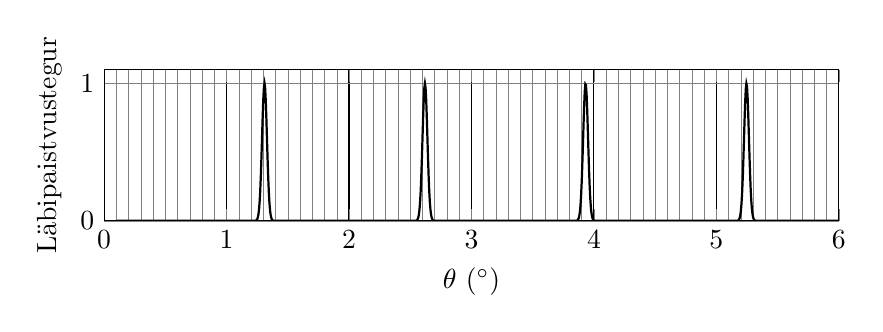
\begin{tikzpicture}
\begin{axis}[
    width=0.9\textwidth,
    height=3.5cm,
    xlabel={$\theta$ ($^\circ$)},
    ylabel={Läbipaistvustegur},
    xmin=0, xmax=6,
    ymin=0, ymax=1.1,
    xtick={0,1,2,3,4,5,6},
    ytick={0,1},
    minor x tick num=9,
    grid=both,
    minor grid style={very thin,gray},
    major x grid style={black},
    major y grid style={very thin,gray},
]

\addplot[color=black,thick]
  coordinates {
  (0.1000,0)
  (0.1050,0)
  (0.1100,0)
  (0.1150,0)
  (0.1200,0)
  (0.1250,0)
  (0.1300,0)
  (0.1350,0)
  (0.1400,0)
  (0.1450,0)
  (0.1500,0)
  (0.1550,0)
  (0.1600,0)
  (0.1650,0)
  (0.1700,0)
  (0.1750,0)
  (0.1800,0)
  (0.1850,0)
  (0.1900,0)
  (0.1950,0)
  (0.2000,0)
  (0.2050,0)
  (0.2100,0)
  (0.2150,0)
  (0.2200,0)
  (0.2250,0)
  (0.2300,0)
  (0.2350,0)
  (0.2400,0)
  (0.2450,0)
  (0.2500,0)
  (0.2550,0)
  (0.2600,0)
  (0.2650,0)
  (0.2700,0)
  (0.2750,0)
  (0.2800,0)
  (0.2850,0)
  (0.2900,0)
  (0.2950,0)
  (0.3000,0)
  (0.3050,0)
  (0.3100,0)
  (0.3150,0)
  (0.3200,0)
  (0.3250,0)
  (0.3300,0)
  (0.3350,0)
  (0.3400,0)
  (0.3450,0)
  (0.3500,0)
  (0.3550,0)
  (0.3600,0)
  (0.3650,0)
  (0.3700,0)
  (0.3750,0)
  (0.3800,0)
  (0.3850,0)
  (0.3900,0)
  (0.3950,0)
  (0.4000,0)
  (0.4050,0)
  (0.4100,0)
  (0.4150,0)
  (0.4200,0)
  (0.4250,0)
  (0.4300,0)
  (0.4350,0)
  (0.4400,0)
  (0.4450,0)
  (0.4500,0)
  (0.4550,0)
  (0.4600,0)
  (0.4650,0)
  (0.4700,0)
  (0.4750,0)
  (0.4800,0)
  (0.4850,0)
  (0.4900,0)
  (0.4950,0)
  (0.5000,0)
  (0.5050,0)
  (0.5100,0)
  (0.5150,0)
  (0.5200,0)
  (0.5250,0)
  (0.5300,0)
  (0.5350,0)
  (0.5400,0.0000)
  (0.5450,0.0000)
  (0.5500,0.0000)
  (0.5550,0.0000)
  (0.5600,0.0000)
  (0.5650,0.0000)
  (0.5700,0.0000)
  (0.5750,0.0000)
  (0.5800,0.0000)
  (0.5850,0.0000)
  (0.5900,0.0000)
  (0.5950,0.0000)
  (0.6000,0.0000)
  (0.6050,0.0000)
  (0.6100,0.0000)
  (0.6150,0.0000)
  (0.6200,0.0000)
  (0.6250,0.0000)
  (0.6300,0.0000)
  (0.6350,0.0000)
  (0.6400,0.0000)
  (0.6450,0.0000)
  (0.6500,0.0000)
  (0.6550,0.0000)
  (0.6600,0.0000)
  (0.6650,0.0000)
  (0.6700,0.0000)
  (0.6750,0.0000)
  (0.6800,0.0000)
  (0.6850,0.0000)
  (0.6900,0.0000)
  (0.6950,0.0000)
  (0.7000,0.0000)
  (0.7050,0.0000)
  (0.7100,0.0000)
  (0.7150,0.0000)
  (0.7200,0.0000)
  (0.7250,0.0000)
  (0.7300,0.0000)
  (0.7350,0.0000)
  (0.7400,0.0000)
  (0.7450,0.0000)
  (0.7500,0.0000)
  (0.7550,0.0000)
  (0.7600,0.0000)
  (0.7650,0.0000)
  (0.7700,0.0000)
  (0.7750,0.0000)
  (0.7800,0.0000)
  (0.7850,0.0000)
  (0.7900,0.0000)
  (0.7950,0.0000)
  (0.8000,0.0000)
  (0.8050,0.0000)
  (0.8100,0.0000)
  (0.8150,0.0000)
  (0.8200,0.0000)
  (0.8250,0.0000)
  (0.8300,0.0000)
  (0.8350,0.0000)
  (0.8400,0.0000)
  (0.8450,0.0000)
  (0.8500,0.0000)
  (0.8550,0.0000)
  (0.8600,0.0000)
  (0.8650,0.0000)
  (0.8700,0.0000)
  (0.8750,0.0000)
  (0.8800,0.0000)
  (0.8850,0.0000)
  (0.8900,0.0000)
  (0.8950,0.0000)
  (0.9000,0.0000)
  (0.9050,0.0000)
  (0.9100,0.0000)
  (0.9150,0.0000)
  (0.9200,0.0000)
  (0.9250,0.0000)
  (0.9300,0.0000)
  (0.9350,0.0000)
  (0.9400,0.0000)
  (0.9450,0.0000)
  (0.9500,0.0000)
  (0.9550,0.0000)
  (0.9600,0.0000)
  (0.9650,0.0000)
  (0.9700,0.0000)
  (0.9750,0.0000)
  (0.9800,0.0000)
  (0.9850,0.0000)
  (0.9900,0.0000)
  (0.9950,0.0000)
  (1.0000,0.0000)
  (1.0050,0.0000)
  (1.0100,0.0000)
  (1.0150,0.0000)
  (1.0200,0.0000)
  (1.0250,0.0000)
  (1.0300,0.0000)
  (1.0350,0.0000)
  (1.0400,0.0000)
  (1.0450,0.0000)
  (1.0500,0.0000)
  (1.0550,0.0000)
  (1.0600,0.0000)
  (1.0650,0.0000)
  (1.0700,0.0000)
  (1.0750,0.0000)
  (1.0800,0.0000)
  (1.0850,0.0000)
  (1.0900,0.0000)
  (1.0950,0.0000)
  (1.1000,0.0000)
  (1.1050,0.0000)
  (1.1100,0.0000)
  (1.1150,0.0000)
  (1.1200,0.0000)
  (1.1250,0.0000)
  (1.1300,0.0000)
  (1.1350,0.0000)
  (1.1400,0.0000)
  (1.1450,0.0000)
  (1.1500,0.0000)
  (1.1550,0.0000)
  (1.1600,0.0000)
  (1.1650,0.0000)
  (1.1700,0.0000)
  (1.1750,0.0000)
  (1.1800,0.0000)
  (1.1850,0.0000)
  (1.1900,0.0000)
  (1.1950,0.0000)
  (1.2000,0.0000)
  (1.2050,0.0000)
  (1.2100,0.0000)
  (1.2150,0.0000)
  (1.2200,0.0000)
  (1.2250,0.0001)
  (1.2300,0.0004)
  (1.2350,0.0009)
  (1.2400,0.0023)
  (1.2450,0.0053)
  (1.2500,0.0116)
  (1.2550,0.0236)
  (1.2600,0.0454)
  (1.2650,0.0820)
  (1.2700,0.1390)
  (1.2750,0.2214)
  (1.2800,0.3312)
  (1.2850,0.4655)
  (1.2900,0.6147)
  (1.2950,0.7624)
  (1.3000,0.8884)
  (1.3050,0.9724)
  (1.3100,0.9999)
  (1.3150,0.9659)
  (1.3200,0.8765)
  (1.3250,0.7472)
  (1.3300,0.5984)
  (1.3350,0.4502)
  (1.3400,0.3182)
  (1.3450,0.2112)
  (1.3500,0.1317)
  (1.3550,0.0772)
  (1.3600,0.0425)
  (1.3650,0.0220)
  (1.3700,0.0107)
  (1.3750,0.0049)
  (1.3800,0.0021)
  (1.3850,0.0008)
  (1.3900,0.0003)
  (1.3950,0.0001)
  (1.4000,0.0000)
  (1.4050,0.0000)
  (1.4100,0.0000)
  (1.4150,0.0000)
  (1.4200,0.0000)
  (1.4250,0.0000)
  (1.4300,0.0000)
  (1.4350,0.0000)
  (1.4400,0.0000)
  (1.4450,0.0000)
  (1.4500,0.0000)
  (1.4550,0.0000)
  (1.4600,0.0000)
  (1.4650,0.0000)
  (1.4700,0.0000)
  (1.4750,0.0000)
  (1.4800,0.0000)
  (1.4850,0.0000)
  (1.4900,0.0000)
  (1.4950,0.0000)
  (1.5000,0.0000)
  (1.5050,0.0000)
  (1.5100,0.0000)
  (1.5150,0.0000)
  (1.5200,0.0000)
  (1.5250,0.0000)
  (1.5300,0.0000)
  (1.5350,0.0000)
  (1.5400,0.0000)
  (1.5450,0.0000)
  (1.5500,0.0000)
  (1.5550,0.0000)
  (1.5600,0.0000)
  (1.5650,0.0000)
  (1.5700,0.0000)
  (1.5750,0.0000)
  (1.5800,0.0000)
  (1.5850,0.0000)
  (1.5900,0.0000)
  (1.5950,0.0000)
  (1.6000,0.0000)
  (1.6050,0.0000)
  (1.6100,0.0000)
  (1.6150,0.0000)
  (1.6200,0.0000)
  (1.6250,0.0000)
  (1.6300,0.0000)
  (1.6350,0.0000)
  (1.6400,0.0000)
  (1.6450,0.0000)
  (1.6500,0.0000)
  (1.6550,0.0000)
  (1.6600,0.0000)
  (1.6650,0.0000)
  (1.6700,0.0000)
  (1.6750,0.0000)
  (1.6800,0.0000)
  (1.6850,0.0000)
  (1.6900,0.0000)
  (1.6950,0.0000)
  (1.7000,0.0000)
  (1.7050,0.0000)
  (1.7100,0.0000)
  (1.7150,0.0000)
  (1.7200,0.0000)
  (1.7250,0.0000)
  (1.7300,0.0000)
  (1.7350,0.0000)
  (1.7400,0.0000)
  (1.7450,0.0000)
  (1.7500,0.0000)
  (1.7550,0.0000)
  (1.7600,0.0000)
  (1.7650,0.0000)
  (1.7700,0.0000)
  (1.7750,0.0000)
  (1.7800,0.0000)
  (1.7850,0.0000)
  (1.7900,0.0000)
  (1.7950,0.0000)
  (1.8000,0.0000)
  (1.8050,0.0000)
  (1.8100,0.0000)
  (1.8150,0.0000)
  (1.8200,0.0000)
  (1.8250,0.0000)
  (1.8300,0.0000)
  (1.8350,0.0000)
  (1.8400,0.0000)
  (1.8450,0.0000)
  (1.8500,0.0000)
  (1.8550,0.0000)
  (1.8600,0.0000)
  (1.8650,0.0000)
  (1.8700,0.0000)
  (1.8750,0.0000)
  (1.8800,0.0000)
  (1.8850,0.0000)
  (1.8900,0.0000)
  (1.8950,0.0000)
  (1.9000,0.0000)
  (1.9050,0.0000)
  (1.9100,0.0000)
  (1.9150,0.0000)
  (1.9200,0.0000)
  (1.9250,0.0000)
  (1.9300,0.0000)
  (1.9350,0.0000)
  (1.9400,0.0000)
  (1.9450,0.0000)
  (1.9500,0.0000)
  (1.9550,0.0000)
  (1.9600,0.0000)
  (1.9650,0.0000)
  (1.9700,0.0000)
  (1.9750,0.0000)
  (1.9800,0.0000)
  (1.9850,0.0000)
  (1.9900,0.0000)
  (1.9950,0.0000)
  (2.0000,0.0000)
  (2.0050,0.0000)
  (2.0100,0.0000)
  (2.0150,0.0000)
  (2.0200,0.0000)
  (2.0250,0.0000)
  (2.0300,0.0000)
  (2.0350,0.0000)
  (2.0400,0.0000)
  (2.0450,0.0000)
  (2.0500,0.0000)
  (2.0550,0.0000)
  (2.0600,0.0000)
  (2.0650,0.0000)
  (2.0700,0.0000)
  (2.0750,0.0000)
  (2.0800,0.0000)
  (2.0850,0.0000)
  (2.0900,0.0000)
  (2.0950,0.0000)
  (2.1000,0.0000)
  (2.1050,0.0000)
  (2.1100,0.0000)
  (2.1150,0.0000)
  (2.1200,0.0000)
  (2.1250,0.0000)
  (2.1300,0.0000)
  (2.1350,0.0000)
  (2.1400,0.0000)
  (2.1450,0.0000)
  (2.1500,0.0000)
  (2.1550,0.0000)
  (2.1600,0.0000)
  (2.1650,0.0000)
  (2.1700,0.0000)
  (2.1750,0.0000)
  (2.1800,0.0000)
  (2.1850,0.0000)
  (2.1900,0.0000)
  (2.1950,0.0000)
  (2.2000,0.0000)
  (2.2050,0.0000)
  (2.2100,0.0000)
  (2.2150,0.0000)
  (2.2200,0.0000)
  (2.2250,0.0000)
  (2.2300,0.0000)
  (2.2350,0.0000)
  (2.2400,0.0000)
  (2.2450,0.0000)
  (2.2500,0.0000)
  (2.2550,0.0000)
  (2.2600,0.0000)
  (2.2650,0.0000)
  (2.2700,0.0000)
  (2.2750,0.0000)
  (2.2800,0.0000)
  (2.2850,0.0000)
  (2.2900,0.0000)
  (2.2950,0.0000)
  (2.3000,0.0000)
  (2.3050,0.0000)
  (2.3100,0.0000)
  (2.3150,0.0000)
  (2.3200,0.0000)
  (2.3250,0.0000)
  (2.3300,0.0000)
  (2.3350,0.0000)
  (2.3400,0.0000)
  (2.3450,0.0000)
  (2.3500,0.0000)
  (2.3550,0.0000)
  (2.3600,0.0000)
  (2.3650,0.0000)
  (2.3700,0.0000)
  (2.3750,0.0000)
  (2.3800,0.0000)
  (2.3850,0.0000)
  (2.3900,0.0000)
  (2.3950,0.0000)
  (2.4000,0.0000)
  (2.4050,0.0000)
  (2.4100,0.0000)
  (2.4150,0.0000)
  (2.4200,0.0000)
  (2.4250,0.0000)
  (2.4300,0.0000)
  (2.4350,0.0000)
  (2.4400,0.0000)
  (2.4450,0.0000)
  (2.4500,0.0000)
  (2.4550,0.0000)
  (2.4600,0.0000)
  (2.4650,0.0000)
  (2.4700,0.0000)
  (2.4750,0.0000)
  (2.4800,0.0000)
  (2.4850,0.0000)
  (2.4900,0.0000)
  (2.4950,0.0000)
  (2.5000,0.0000)
  (2.5050,0.0000)
  (2.5100,0.0000)
  (2.5150,0.0000)
  (2.5200,0.0000)
  (2.5250,0.0000)
  (2.5300,0.0000)
  (2.5350,0.0001)
  (2.5400,0.0003)
  (2.5450,0.0009)
  (2.5500,0.0021)
  (2.5550,0.0050)
  (2.5600,0.0109)
  (2.5650,0.0223)
  (2.5700,0.0431)
  (2.5750,0.0782)
  (2.5800,0.1333)
  (2.5850,0.2135)
  (2.5900,0.3211)
  (2.5950,0.4536)
  (2.6000,0.6020)
  (2.6050,0.7506)
  (2.6100,0.8792)
  (2.6150,0.9674)
  (2.6200,1.0000)
  (2.6250,0.9710)
  (2.6300,0.8858)
  (2.6350,0.7591)
  (2.6400,0.6111)
  (2.6450,0.4621)
  (2.6500,0.3283)
  (2.6550,0.2191)
  (2.6600,0.1374)
  (2.6650,0.0809)
  (2.6700,0.0448)
  (2.6750,0.0233)
  (2.6800,0.0114)
  (2.6850,0.0052)
  (2.6900,0.0022)
  (2.6950,0.0009)
  (2.7000,0.0003)
  (2.7050,0.0001)
  (2.7100,0.0000)
  (2.7150,0.0000)
  (2.7200,0.0000)
  (2.7250,0.0000)
  (2.7300,0.0000)
  (2.7350,0.0000)
  (2.7400,0.0000)
  (2.7450,0.0000)
  (2.7500,0.0000)
  (2.7550,0.0000)
  (2.7600,0.0000)
  (2.7650,0.0000)
  (2.7700,0.0000)
  (2.7750,0.0000)
  (2.7800,0.0000)
  (2.7850,0.0000)
  (2.7900,0.0000)
  (2.7950,0.0000)
  (2.8000,0.0000)
  (2.8050,0.0000)
  (2.8100,0.0000)
  (2.8150,0.0000)
  (2.8200,0.0000)
  (2.8250,0.0000)
  (2.8300,0.0000)
  (2.8350,0.0000)
  (2.8400,0.0000)
  (2.8450,0.0000)
  (2.8500,0.0000)
  (2.8550,0.0000)
  (2.8600,0.0000)
  (2.8650,0.0000)
  (2.8700,0.0000)
  (2.8750,0.0000)
  (2.8800,0.0000)
  (2.8850,0.0000)
  (2.8900,0.0000)
  (2.8950,0.0000)
  (2.9000,0.0000)
  (2.9050,0.0000)
  (2.9100,0.0000)
  (2.9150,0.0000)
  (2.9200,0.0000)
  (2.9250,0.0000)
  (2.9300,0.0000)
  (2.9350,0.0000)
  (2.9400,0.0000)
  (2.9450,0.0000)
  (2.9500,0.0000)
  (2.9550,0.0000)
  (2.9600,0.0000)
  (2.9650,0.0000)
  (2.9700,0.0000)
  (2.9750,0.0000)
  (2.9800,0.0000)
  (2.9850,0.0000)
  (2.9900,0.0000)
  (2.9950,0.0000)
  (3.0000,0.0000)
  (3.0050,0.0000)
  (3.0100,0.0000)
  (3.0150,0.0000)
  (3.0200,0.0000)
  (3.0250,0.0000)
  (3.0300,0.0000)
  (3.0350,0.0000)
  (3.0400,0.0000)
  (3.0450,0.0000)
  (3.0500,0.0000)
  (3.0550,0.0000)
  (3.0600,0.0000)
  (3.0650,0.0000)
  (3.0700,0.0000)
  (3.0750,0.0000)
  (3.0800,0.0000)
  (3.0850,0.0000)
  (3.0900,0.0000)
  (3.0950,0.0000)
  (3.1000,0.0000)
  (3.1050,0.0000)
  (3.1100,0.0000)
  (3.1150,0.0000)
  (3.1200,0.0000)
  (3.1250,0.0000)
  (3.1300,0.0000)
  (3.1350,0.0000)
  (3.1400,0.0000)
  (3.1450,0.0000)
  (3.1500,0.0000)
  (3.1550,0.0000)
  (3.1600,0.0000)
  (3.1650,0.0000)
  (3.1700,0.0000)
  (3.1750,0.0000)
  (3.1800,0.0000)
  (3.1850,0.0000)
  (3.1900,0.0000)
  (3.1950,0.0000)
  (3.2000,0.0000)
  (3.2050,0.0000)
  (3.2100,0.0000)
  (3.2150,0.0000)
  (3.2200,0.0000)
  (3.2250,0.0000)
  (3.2300,0.0000)
  (3.2350,0.0000)
  (3.2400,0.0000)
  (3.2450,0.0000)
  (3.2500,0.0000)
  (3.2550,0.0000)
  (3.2600,0.0000)
  (3.2650,0.0000)
  (3.2700,0.0000)
  (3.2750,0.0000)
  (3.2800,0.0000)
  (3.2850,0.0000)
  (3.2900,0.0000)
  (3.2950,0.0000)
  (3.3000,0.0000)
  (3.3050,0.0000)
  (3.3100,0.0000)
  (3.3150,0.0000)
  (3.3200,0.0000)
  (3.3250,0.0000)
  (3.3300,0.0000)
  (3.3350,0.0000)
  (3.3400,0.0000)
  (3.3450,0.0000)
  (3.3500,0.0000)
  (3.3550,0.0000)
  (3.3600,0.0000)
  (3.3650,0.0000)
  (3.3700,0.0000)
  (3.3750,0.0000)
  (3.3800,0.0000)
  (3.3850,0.0000)
  (3.3900,0.0000)
  (3.3950,0.0000)
  (3.4000,0.0000)
  (3.4050,0.0000)
  (3.4100,0.0000)
  (3.4150,0.0000)
  (3.4200,0.0000)
  (3.4250,0.0000)
  (3.4300,0.0000)
  (3.4350,0.0000)
  (3.4400,0.0000)
  (3.4450,0.0000)
  (3.4500,0.0000)
  (3.4550,0.0000)
  (3.4600,0.0000)
  (3.4650,0.0000)
  (3.4700,0.0000)
  (3.4750,0.0000)
  (3.4800,0.0000)
  (3.4850,0.0000)
  (3.4900,0.0000)
  (3.4950,0.0000)
  (3.5000,0.0000)
  (3.5050,0.0000)
  (3.5100,0.0000)
  (3.5150,0.0000)
  (3.5200,0.0000)
  (3.5250,0.0000)
  (3.5300,0.0000)
  (3.5350,0.0000)
  (3.5400,0.0000)
  (3.5450,0.0000)
  (3.5500,0.0000)
  (3.5550,0.0000)
  (3.5600,0.0000)
  (3.5650,0.0000)
  (3.5700,0.0000)
  (3.5750,0.0000)
  (3.5800,0.0000)
  (3.5850,0.0000)
  (3.5900,0.0000)
  (3.5950,0.0000)
  (3.6000,0.0000)
  (3.6050,0.0000)
  (3.6100,0.0000)
  (3.6150,0.0000)
  (3.6200,0.0000)
  (3.6250,0.0000)
  (3.6300,0.0000)
  (3.6350,0.0000)
  (3.6400,0.0000)
  (3.6450,0.0000)
  (3.6500,0.0000)
  (3.6550,0.0000)
  (3.6600,0.0000)
  (3.6650,0.0000)
  (3.6700,0.0000)
  (3.6750,0.0000)
  (3.6800,0.0000)
  (3.6850,0.0000)
  (3.6900,0.0000)
  (3.6950,0.0000)
  (3.7000,0.0000)
  (3.7050,0.0000)
  (3.7100,0.0000)
  (3.7150,0.0000)
  (3.7200,0.0000)
  (3.7250,0.0000)
  (3.7300,0.0000)
  (3.7350,0.0000)
  (3.7400,0.0000)
  (3.7450,0.0000)
  (3.7500,0.0000)
  (3.7550,0.0000)
  (3.7600,0.0000)
  (3.7650,0.0000)
  (3.7700,0.0000)
  (3.7750,0.0000)
  (3.7800,0.0000)
  (3.7850,0.0000)
  (3.7900,0.0000)
  (3.7950,0.0000)
  (3.8000,0.0000)
  (3.8050,0.0000)
  (3.8100,0.0000)
  (3.8150,0.0000)
  (3.8200,0.0000)
  (3.8250,0.0000)
  (3.8300,0.0000)
  (3.8350,0.0000)
  (3.8400,0.0000)
  (3.8450,0.0001)
  (3.8500,0.0002)
  (3.8550,0.0006)
  (3.8600,0.0016)
  (3.8650,0.0037)
  (3.8700,0.0083)
  (3.8750,0.0174)
  (3.8800,0.0343)
  (3.8850,0.0637)
  (3.8900,0.1110)
  (3.8950,0.1817)
  (3.9000,0.2794)
  (3.9050,0.4037)
  (3.9100,0.5479)
  (3.9150,0.6986)
  (3.9200,0.8368)
  (3.9250,0.9416)
  (3.9300,0.9953)
  (3.9350,0.9884)
  (3.9400,0.9220)
  (3.9450,0.8080)
  (3.9500,0.6652)
  (3.9550,0.5144)
  (3.9600,0.3737)
  (3.9650,0.2551)
  (3.9700,0.1635)
  (3.9750,0.0985)
  (3.9800,0.0557)
  (3.9850,0.0296)
  (3.9900,0.0148)
  (3.9950,0.0069)
  (4.0000,0.0031)
  (4.0050,0.0013)
  (4.0100,0.0005)
  (4.0150,0.0002)
  (4.0200,0.0001)
  (4.0250,0.0000)
  (4.0300,0.0000)
  (4.0350,0.0000)
  (4.0400,0.0000)
  (4.0450,0.0000)
  (4.0500,0.0000)
  (4.0550,0.0000)
  (4.0600,0.0000)
  (4.0650,0.0000)
  (4.0700,0.0000)
  (4.0750,0.0000)
  (4.0800,0.0000)
  (4.0850,0.0000)
  (4.0900,0.0000)
  (4.0950,0.0000)
  (4.1000,0.0000)
  (4.1050,0.0000)
  (4.1100,0.0000)
  (4.1150,0.0000)
  (4.1200,0.0000)
  (4.1250,0.0000)
  (4.1300,0.0000)
  (4.1350,0.0000)
  (4.1400,0.0000)
  (4.1450,0.0000)
  (4.1500,0.0000)
  (4.1550,0.0000)
  (4.1600,0.0000)
  (4.1650,0.0000)
  (4.1700,0.0000)
  (4.1750,0.0000)
  (4.1800,0.0000)
  (4.1850,0.0000)
  (4.1900,0.0000)
  (4.1950,0.0000)
  (4.2000,0.0000)
  (4.2050,0.0000)
  (4.2100,0.0000)
  (4.2150,0.0000)
  (4.2200,0.0000)
  (4.2250,0.0000)
  (4.2300,0.0000)
  (4.2350,0.0000)
  (4.2400,0.0000)
  (4.2450,0.0000)
  (4.2500,0.0000)
  (4.2550,0.0000)
  (4.2600,0.0000)
  (4.2650,0.0000)
  (4.2700,0.0000)
  (4.2750,0.0000)
  (4.2800,0.0000)
  (4.2850,0.0000)
  (4.2900,0.0000)
  (4.2950,0.0000)
  (4.3000,0.0000)
  (4.3050,0.0000)
  (4.3100,0.0000)
  (4.3150,0.0000)
  (4.3200,0.0000)
  (4.3250,0.0000)
  (4.3300,0.0000)
  (4.3350,0.0000)
  (4.3400,0.0000)
  (4.3450,0.0000)
  (4.3500,0.0000)
  (4.3550,0.0000)
  (4.3600,0.0000)
  (4.3650,0.0000)
  (4.3700,0.0000)
  (4.3750,0.0000)
  (4.3800,0.0000)
  (4.3850,0.0000)
  (4.3900,0.0000)
  (4.3950,0.0000)
  (4.4000,0.0000)
  (4.4050,0.0000)
  (4.4100,0.0000)
  (4.4150,0.0000)
  (4.4200,0.0000)
  (4.4250,0.0000)
  (4.4300,0.0000)
  (4.4350,0.0000)
  (4.4400,0.0000)
  (4.4450,0.0000)
  (4.4500,0.0000)
  (4.4550,0.0000)
  (4.4600,0.0000)
  (4.4650,0.0000)
  (4.4700,0.0000)
  (4.4750,0.0000)
  (4.4800,0.0000)
  (4.4850,0.0000)
  (4.4900,0.0000)
  (4.4950,0.0000)
  (4.5000,0.0000)
  (4.5050,0.0000)
  (4.5100,0.0000)
  (4.5150,0.0000)
  (4.5200,0.0000)
  (4.5250,0.0000)
  (4.5300,0.0000)
  (4.5350,0.0000)
  (4.5400,0.0000)
  (4.5450,0.0000)
  (4.5500,0.0000)
  (4.5550,0.0000)
  (4.5600,0.0000)
  (4.5650,0.0000)
  (4.5700,0.0000)
  (4.5750,0.0000)
  (4.5800,0.0000)
  (4.5850,0.0000)
  (4.5900,0.0000)
  (4.5950,0.0000)
  (4.6000,0.0000)
  (4.6050,0.0000)
  (4.6100,0.0000)
  (4.6150,0.0000)
  (4.6200,0.0000)
  (4.6250,0.0000)
  (4.6300,0.0000)
  (4.6350,0.0000)
  (4.6400,0.0000)
  (4.6450,0.0000)
  (4.6500,0.0000)
  (4.6550,0.0000)
  (4.6600,0.0000)
  (4.6650,0.0000)
  (4.6700,0.0000)
  (4.6750,0.0000)
  (4.6800,0.0000)
  (4.6850,0.0000)
  (4.6900,0.0000)
  (4.6950,0.0000)
  (4.7000,0.0000)
  (4.7050,0.0000)
  (4.7100,0.0000)
  (4.7150,0.0000)
  (4.7200,0.0000)
  (4.7250,0.0000)
  (4.7300,0.0000)
  (4.7350,0.0000)
  (4.7400,0.0000)
  (4.7450,0.0000)
  (4.7500,0.0000)
  (4.7550,0.0000)
  (4.7600,0.0000)
  (4.7650,0.0000)
  (4.7700,0.0000)
  (4.7750,0.0000)
  (4.7800,0.0000)
  (4.7850,0.0000)
  (4.7900,0.0000)
  (4.7950,0.0000)
  (4.8000,0.0000)
  (4.8050,0.0000)
  (4.8100,0.0000)
  (4.8150,0.0000)
  (4.8200,0.0000)
  (4.8250,0.0000)
  (4.8300,0.0000)
  (4.8350,0.0000)
  (4.8400,0.0000)
  (4.8450,0.0000)
  (4.8500,0.0000)
  (4.8550,0.0000)
  (4.8600,0.0000)
  (4.8650,0.0000)
  (4.8700,0.0000)
  (4.8750,0.0000)
  (4.8800,0.0000)
  (4.8850,0.0000)
  (4.8900,0.0000)
  (4.8950,0.0000)
  (4.9000,0.0000)
  (4.9050,0.0000)
  (4.9100,0.0000)
  (4.9150,0.0000)
  (4.9200,0.0000)
  (4.9250,0.0000)
  (4.9300,0.0000)
  (4.9350,0.0000)
  (4.9400,0.0000)
  (4.9450,0.0000)
  (4.9500,0.0000)
  (4.9550,0.0000)
  (4.9600,0.0000)
  (4.9650,0.0000)
  (4.9700,0.0000)
  (4.9750,0.0000)
  (4.9800,0.0000)
  (4.9850,0.0000)
  (4.9900,0.0000)
  (4.9950,0.0000)
  (5.0000,0.0000)
  (5.0050,0.0000)
  (5.0100,0.0000)
  (5.0150,0.0000)
  (5.0200,0.0000)
  (5.0250,0.0000)
  (5.0300,0.0000)
  (5.0350,0.0000)
  (5.0400,0.0000)
  (5.0450,0.0000)
  (5.0500,0.0000)
  (5.0550,0.0000)
  (5.0600,0.0000)
  (5.0650,0.0000)
  (5.0700,0.0000)
  (5.0750,0.0000)
  (5.0800,0.0000)
  (5.0850,0.0000)
  (5.0900,0.0000)
  (5.0950,0.0000)
  (5.1000,0.0000)
  (5.1050,0.0000)
  (5.1100,0.0000)
  (5.1150,0.0000)
  (5.1200,0.0000)
  (5.1250,0.0000)
  (5.1300,0.0000)
  (5.1350,0.0000)
  (5.1400,0.0000)
  (5.1450,0.0000)
  (5.1500,0.0000)
  (5.1550,0.0000)
  (5.1600,0.0001)
  (5.1650,0.0003)
  (5.1700,0.0008)
  (5.1750,0.0019)
  (5.1800,0.0045)
  (5.1850,0.0098)
  (5.1900,0.0204)
  (5.1950,0.0397)
  (5.2000,0.0727)
  (5.2050,0.1249)
  (5.2100,0.2015)
  (5.2150,0.3056)
  (5.2200,0.4353)
  (5.2250,0.5824)
  (5.2300,0.7320)
  (5.2350,0.8644)
  (5.2400,0.9589)
  (5.2450,0.9992)
  (5.2500,0.9782)
  (5.2550,0.8996)
  (5.2600,0.7771)
  (5.2650,0.6307)
  (5.2700,0.4809)
  (5.2750,0.3444)
  (5.2800,0.2317)
  (5.2850,0.1465)
  (5.2900,0.0870)
  (5.2950,0.0485)
  (5.3000,0.0254)
  (5.3050,0.0125)
  (5.3100,0.0058)
  (5.3150,0.0025)
  (5.3200,0.0010)
  (5.3250,0.0004)
  (5.3300,0.0001)
  (5.3350,0.0000)
  (5.3400,0.0000)
  (5.3450,0.0000)
  (5.3500,0.0000)
  (5.3550,0.0000)
  (5.3600,0.0000)
  (5.3650,0.0000)
  (5.3700,0.0000)
  (5.3750,0.0000)
  (5.3800,0.0000)
  (5.3850,0.0000)
  (5.3900,0.0000)
  (5.3950,0.0000)
  (5.4000,0.0000)
  (5.4050,0.0000)
  (5.4100,0.0000)
  (5.4150,0.0000)
  (5.4200,0.0000)
  (5.4250,0.0000)
  (5.4300,0.0000)
  (5.4350,0.0000)
  (5.4400,0.0000)
  (5.4450,0.0000)
  (5.4500,0.0000)
  (5.4550,0.0000)
  (5.4600,0.0000)
  (5.4650,0.0000)
  (5.4700,0.0000)
  (5.4750,0.0000)
  (5.4800,0.0000)
  (5.4850,0.0000)
  (5.4900,0.0000)
  (5.4950,0.0000)
  (5.5000,0.0000)
  (5.5050,0.0000)
  (5.5100,0.0000)
  (5.5150,0.0000)
  (5.5200,0.0000)
  (5.5250,0.0000)
  (5.5300,0.0000)
  (5.5350,0.0000)
  (5.5400,0.0000)
  (5.5450,0.0000)
  (5.5500,0.0000)
  (5.5550,0.0000)
  (5.5600,0.0000)
  (5.5650,0.0000)
  (5.5700,0.0000)
  (5.5750,0.0000)
  (5.5800,0.0000)
  (5.5850,0.0000)
  (5.5900,0.0000)
  (5.5950,0.0000)
  (5.6000,0.0000)
  (5.6050,0.0000)
  (5.6100,0.0000)
  (5.6150,0.0000)
  (5.6200,0.0000)
  (5.6250,0.0000)
  (5.6300,0.0000)
  (5.6350,0.0000)
  (5.6400,0.0000)
  (5.6450,0.0000)
  (5.6500,0.0000)
  (5.6550,0.0000)
  (5.6600,0.0000)
  (5.6650,0.0000)
  (5.6700,0.0000)
  (5.6750,0.0000)
  (5.6800,0.0000)
  (5.6850,0.0000)
  (5.6900,0.0000)
  (5.6950,0.0000)
  (5.7000,0.0000)
  (5.7050,0.0000)
  (5.7100,0.0000)
  (5.7150,0.0000)
  (5.7200,0.0000)
  (5.7250,0.0000)
  (5.7300,0.0000)
  (5.7350,0.0000)
  (5.7400,0.0000)
  (5.7450,0.0000)
  (5.7500,0.0000)
  (5.7550,0.0000)
  (5.7600,0.0000)
  (5.7650,0.0000)
  (5.7700,0.0000)
  (5.7750,0.0000)
  (5.7800,0.0000)
  (5.7850,0.0000)
  (5.7900,0.0000)
  (5.7950,0.0000)
  (5.8000,0.0000)
  (5.8050,0.0000)
  (5.8100,0.0000)
  (5.8150,0.0000)
  (5.8200,0.0000)
  (5.8250,0.0000)
  (5.8300,0.0000)
  (5.8350,0.0000)
  (5.8400,0.0000)
  (5.8450,0.0000)
  (5.8500,0.0000)
  (5.8550,0.0000)
  (5.8600,0.0000)
  (5.8650,0.0000)
  (5.8700,0.0000)
  (5.8750,0.0000)
  (5.8800,0.0000)
  (5.8850,0.0000)
  (5.8900,0.0000)
  (5.8950,0.0000)
  (5.9000,0.0000)
  (5.9050,0.0000)
  (5.9100,0.0000)
  (5.9150,0.0000)
  (5.9200,0.0000)
  (5.9250,0.0000)
  (5.9300,0.0000)
  (5.9350,0.0000)
  (5.9400,0.0000)
  (5.9450,0.0000)
  (5.9500,0.0000)
  (5.9550,0.0000)
  (5.9600,0.0000)
  (5.9650,0.0000)
  (5.9700,0.0000)
  (5.9750,0.0000)
  (5.9800,0.0000)
  (5.9850,0.0000)
  (5.9900,0.0000)
  (5.9950,0.0000)
  (6.0000,0.0000)
  };
\end{axis}
\end{tikzpicture}

	\vspace{-45pt}
\end{figure}
\probend
\bigskip

% Ü143
\setAuthor{Taavet Kalda}
\setRound{lõppvoor}
\setYear{2021}
\setNumber{G 8}
\setDifficulty{8}
\setTopic{TODO}

\prob{Veesilinder}
Mihkel täidab silindrilise anuma kõrgusega $h = \SI{12}{\m}$ täielikult veega. Seejärel ta katab silindri kaanega, ning pöörab selle tagurpidi. Missuguse kiirendusega hakkab vesi silindrist välja voolama, kui Mihkel silindri alt kaane ära võtab? Küllastunud veeauru rõhk toatemperatuuril on $p_v = \SI{3170}{\Pa}$, vee tihedus $\rho = \SI{1000}{\kg\per\m\cubed}$, atmosfääri rõhk $p_0 = \SI{101325}{\Pa}$, raskuskiirendus $g = \SI{9.8}{\m\per\s\squared}$.
\probend
\bigskip

% Ü144
\setAuthor{Päivo Simson}
\setRound{lahtine}
\setYear{2022}
\setNumber{G 8}
\setDifficulty{8}
\setTopic{TODO}

\prob{Kaubalaev}
Lastimise käigus hakkab kaubalaev tasases vees väikse amplituudiga üles-alla võnkuma. Kui laevale on tõstetud $m_1 = \SI{1000}{}$ tonni kaupa, on võnkumiste sagedus $f_1 = \SI{10}{}$ võnget minutis. Kui laevale on tõstetud $m_2 = \SI{10000}{}$ tonni kaupa, on võnkumiste sagedus $f_2 = \SI{8}{}$ võnget minutis. On teada, et laeva võnkumine haarab kaasa ka teatud hulga vett, mis näiliselt suurendab laeva inertsi. See tähendab, et vees reageerib laev välisjõududele nii, nagu oleks tema mass kaasahaaratud vee massi võrra tegelikust suurem. Leida laeva tühimass $M$ arvestades, et sõltumata kauba hulgast on kaasahaaratud vee mass $\frac{1}{2}M$. Eeldage, et veepinna lähedal on laeva kere väliskülg vertikaalne.
\probend
\bigskip

% Ü145
\setAuthor{Jaan Kalda}
\setRound{piirkonnavoor}
\setYear{2022}
\setNumber{G 8}
\setDifficulty{8}
\setTopic{TODO}

\prob{Tühi pudel}
Kokapoiss peseb liitrist plastpudelit: laseb sinna natuke kuuma vett temperatuuril $t_v=\qty{55}{\celsius}$, suleb pöidlaga pudelikaela ja raputab tugevasti. Kui ta pöidla nüüd pudeli suu eest ära võtab, käib väike plaksatus ja pudelist surub veidi õhku välja, sest rõhk pudelis oli suurem atmosfäärirõhust. Kui suur oli rõhkude vahe? Toas on õhutemperatuur $t_t=\qty{20}{\celsius}$, suhteline õhuniiskus $r=\qty{50}{\percent}$ ja õhurõhk $p_0=\SI{1.01e5}{Pa}$? Küllastunud veeauru rõhu sõltuvus temperatuurist on toodud juuresoleval graafikul.
\begin{figure}[h]
  \vspace{-0.5em}
  {
    \tikzset{component/.style={draw,thick,circle,fill=white,minimum size=0.75cm,inner sep=0pt}}
    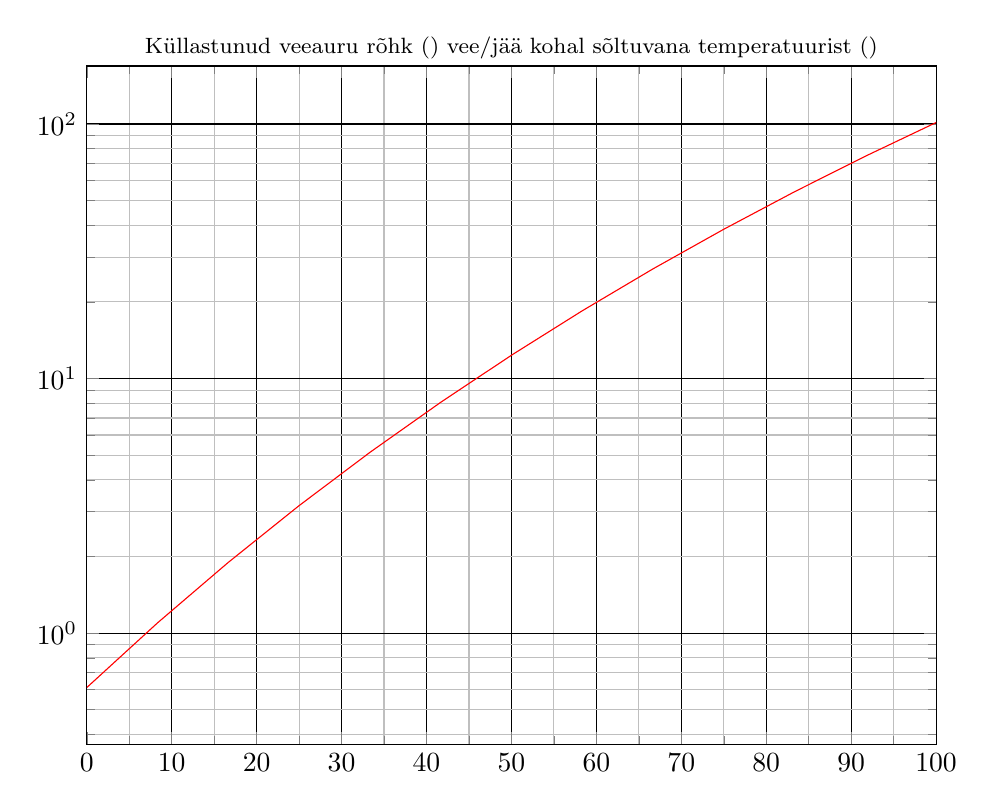
\begin{tikzpicture}
      \begin{axis}[
        ymode=log,
        width=1.02\textwidth,
        height=29em,
        minor tick num=1,
        major grid style = black,
        grid=both,
        % xlabel=$t$ (\unit{\celsius}),
        % ylabel=$P$ (\unit{\kPa}),
        xmin = 0, xmax = 100,
        title={\footnotesize Küllastunud veeauru rõhk (\unit{\kPa}) vee/jää kohal sõltuvana temperatuurist (\unit{\celsius})},
        title style={xshift=0, yshift=-7pt},
        ]
        \addplot[red, domain=0:200] {0.61121*exp((18.678-x/234.5)*(x/(257.14+x)))};
        \addplot[blue, domain=-200:0] {0.61115*exp((23.036-x/333.7)*(x/(279.82+x)))};
      \end{axis}
    \end{tikzpicture}
  }
  \vspace{-1em}
\end{figure}
\probend
\bigskip

% Ü146
\setAuthor{Kaur Aare Saar}
\setRound{lõppvoor}
\setYear{2022}
\setNumber{G 8}
\setDifficulty{8}
\setTopic{TODO}

\prob{Veevalaja}
Oleg seisab kaalul ja ta ühes käes on pudel, kus on $m=\SI{1}{\kilogram}$ vett ja teises käes on piisavalt suur anum, mis on $h=\SI{1}{\meter}$ madalamal kui pudel. Ta hakkab pudelist vett välja valama anumasse kiirusega $\dot{m}=\SI{1}{\kilo\gram / \second}$.
Joonistage graafik (koos arvulise skaalaga), kuidas muutub kaalu näit alates hetkest, kui kogu vesi on veel pudelis kuni hetkeni, kui kogu vesi on jõudnud anumasse. Raskuskiirendus on $g=\SI{10}{\meter / \second\squared}$ ja võib eeldada, et vesi liigub pudelist anumasse ilma õhutakistuseta. Anum on nii lai, et veenivoo seal ei muutu. Tehtud arvutused koos põhjendustega kirjutage eraldi lehele.
\probend
\bigskip

% Ü147
\setAuthor{Valter Kiisk}
\setRound{lahtine}
\setYear{2023}
\setNumber{G 8}
\setDifficulty{8}
\setTopic{TODO}

\prob{Lääts}
\begin{wrapfigure}[8]{r}{0.2\linewidth}
    \vspace{-30pt}
    \begin{center}
        \includegraphics[width=\linewidth]{2023-lahg-08-yl.pdf}
    \end{center}
\end{wrapfigure}
Joonisel on kujutatud teatava tasakumera läätse ristlõige ja selle mõõdud millimeetrites. Lääts on valmistatud klaasist, mille murdumisnäitaja $n=\num{1.52}$.\\
\osa Eeldusel, et kumerpind on sfääriline, kui suur on selle kõverusraadius?\\
\osa Määrake läätse fookuskaugus kiirte jaoks, mis kulgevad optilise peatelje lähedal (Võite eeldada, et lääts on õhuke, st piisab 3 mm täpsusega õigest vastusest.)! \\ \emph{Märkus:} Väikeste nurkade $x$ korral võib kasutada lähendust $\sin{x} \approx \tan{x} \approx x$ (nurk $x$ on radiaanides).
\probend
\bigskip

% Ü148
\setAuthor{Marko Tsengov}
\setRound{piirkonnavoor}
\setYear{2023}
\setNumber{G 8}
\setDifficulty{8}
\setTopic{TODO}

\prob{Süvend ja kera}
\begin{wrapfigure}{r}{0.35\textwidth}
\vspace{-1em}
  \begin{center}
    \includegraphics[width=1\linewidth]{2023-v2g-08-yl.pdf}
  \end{center}
  \vspace{-2em}
\end{wrapfigure}

Tasandil on silindrikujuline süvend raadiusega $r$ ning sügavusega $h$, mis on risti tasandi pinnaga. Süvendi sisse asetatakse kera raadiusega $R$, nii et kera puudutab süvendi keskpunkti ja kera on algselt paigal. Tasand on maapinna suhtes kaldus nurga $\theta$ võrra. Millist tingimust peavad rahuldama antud suurused, et kera saaks mingi arvu põrgete järel süvendist välja hüpata? Võib eeldada, et hõõrdumist ei toimu, põrked on täielikult elastsed, pindade ebatasasuste tõttu on põrkesuunad vähesel määral juhuslikud ning $h < R$.
\probend
\bigskip

% Ü149
\setAuthor{Valter Kiisk}
\setRound{lõppvoor}
\setYear{2023}
\setNumber{G 8}
\setDifficulty{8}
\setTopic{TODO}

\prob{Kuulitõuge}
Nagu mehaanikast hästi teada, lendab visatud keha antud algkiiruse juures (õhutakistuse puudumisel) kõige kaugemale siis, kui viskenurk horisontaali suhtes on \ang{45}. Kuulitõukespordis on optimaalne nurk mõnevõrra väiksem.
\\a) Leidke selle väärtus, eeldades et kuuli maksimaalne lennukaugus on $s_\text{m}=\SI{20}{m}$, tõukaja vabastab kuuli maapinnast kõrgusel $h_0=\SI{2}{m}$ ja algkiirus ei sõltu tõukesuunast.
\\b) Kui suur on sellise kuuli algkiirus?
\\Raskuskiirendus $g=\SI{9.8}{\meter\per\second\squared}$.
\probend
\bigskip

% Ü150
\setAuthor{Jaan Kalda}
\setRound{lahtine}
\setYear{2024}
\setNumber{G 8}
\setDifficulty{8}
\setTopic{TODO}

\prob{Käru}
Kilplased ehitasid käru, mille esimeste ja tagumiste rataste vahel on jõuülekanne: kui esimesi rattaid pöörata päripäeva 8 pööret, teevad tagumised rattad päripäeva 9 pööret. Millise maksimaalse kaldenurgaga teel püsib see käru ilma alla libisemata paigal, kui hõõrdetegur rataste ja tee vahel on  $\mu$ ning esimestele ja tagumistele ratastele mõjub tee poolt ühesugune  toereaktsioon?
\probend
\bigskip

% Ü151
\setAuthor{Hannes Kuslap}
\setRound{piirkonnavoor}
\setYear{2024}
\setNumber{G 8}
\setDifficulty{8}
\setTopic{TODO}

\prob{Hermeetiline saun}
Aivo ehitas sauna $2\times 2\times 3$ meetri suuruse sauna, mille uks on $h=\SI{1.8}{\m}$ kõrge, $l=\SI{0.8}{\m}$ lai ning avaneb sissepoole. Aivo aga polnud väga kogenud ehitaja ja tegi sauna kogemata täielikult hermeetilise, nii et kinnise uksega puudub igasugune õhuvahetus sauna ja väliskeskkonna vahel. Ta pani saunaukse kinni, kui sauna temperatuur oli $T_1 = \SI{20}{\celsius}$, ja küttis seejärel sauna temperatuurini $T_2 = \SI{100}{\celsius}$. Kas Aivo saab nüüd ukse lükates lahti, kui ta kaalub $m=\SI{100}{\kg}$? Võib eeldada, et maksimaalne lükkejõud on piiratud Aivo ja põranda vahelise hõõrde poolt (hõõrdetegur $\mu=\num{0.6}$). Samuti võib eeldada, et väljas on ühtlaselt rõhk $p_0=\SI{101 000}{\Pa}$, sauna soojenemisel kehtib ideaalgaasi võrrand ja ukselink asub ukse servas.
\probend
\bigskip

% Ü152
\setAuthor{Jaan Kalda}
\setRound{lõppvoor}
\setYear{2024}
\setNumber{G 8}
\setDifficulty{8}
\setTopic{TODO}

\prob{Kolmnurk}
Koondav lääts fookuskaugusega $f$ tekitab täisnurksest kolmnurgast, mille üks nurk on $\SI{30}{\degree}$ kujutiseks kolmnurga, mis on samuti täisnurkne ja mille üks nurk on  $\SI{30}{\degree}$. Kolmnurga hüpotenuus kulgeb piki läätse optilist peatelge. Leidke kolmnurga hüpotenuusi pikkus.
\probend
\bigskip

% Ü153
\setAuthor{Jaan Kalda}
\setRound{lahtine}
\setYear{2018}
\setNumber{G 9}
\setDifficulty{9}
\setTopic{TODO}

\prob{Õhkjahutus}
\begin{wrapfigure}[10]{r}{0.4\textwidth}
	\vspace{-20pt}
	\begin{center}
		\includegraphics[width = 0.4\textwidth]{2018-lahg-09-yl.pdf}
	\end{center}
\end{wrapfigure}

\
Valgusdiood tarbib elektrilist võimsust $P=\SI{50}W$. Dioodi jahutamiseks on see kinnitatud vaskplaadile paksusega $t=\SI{500}{\micro m}$. Vase soojusjuhtivustegur $k=\SI{385}{W/m.K}$. Juuresoleval graafikul (suuremalt lisalehel) on toodud plaadi temperatuur sõltuvuses vaadeldava punkti ja dioodi vahelise kauguse naturaallogaritmist. Kauguse mõõtmiseks kasutatud ühikud ei ole teada. Dioodi mõõtmed lugeda tühiselt väikseks. Milline on dioodi kasutegur (milline osa tarvitatud elektrienergiast kiirgub valgusenergiana)?

\textit{Märkus:} soojusjuhtivustegur on arvuliselt võrdne soojusenergiaga, mis kandub materjalis läbi ühikulise ristlõikepindala, kui temperatuur langeb ühe kraadi võrra ühe pikkusühiku kohta.
\probend
\bigskip

% Ü154
\setAuthor{Jaan Kalda}
\setRound{lahtine}
\setYear{2019}
\setNumber{G 9}
\setDifficulty{9}
\setTopic{TODO}

\prob{Hantel}
Kaks metallkera raadiusega $R$ ja massiga $m$ on ühendatud koaksiaalselt metallvardaga, mille pikkus $L$ on hulga suurem $R$-st ja mille mass ning diameeter on tühiselt väiksed. Kogu süsteem asub kaalutuse tingimustes teljega ristsihilises homogeenses magnetväljas induktsiooniga $B$. Ühele kuulikestest kantakse hetkeliselt elektrilaeng $Q$; visandage ühel ja samal joonisel mõlema kuulikese trajektoorid edasise liikumise käigus. Eeldada, et varda elektriline takistus on tühiselt väike ja et $\varepsilon_0B^2L^2R\ll m$, kus $\varepsilon_0$ tähistab vaakumi dielektrilist läbitavust.
\probend
\bigskip

% Ü155
\setAuthor{}
\setRound{piirkonnavoor}
\setYear{2019}
\setNumber{G 9}
\setDifficulty{9}
\setTopic{TODO}

\prob{Kiik}
Juku kiigub  nii suure hooga, et kiik jõuab haripunktis kiigepostide (kiige pöörlemistelje) kõrguseni. Suure hoo tõttu hakkab Juku muretsema, kas kiige postid ikka vastu peavad.\\
\osa Leida minimaalne ja maksimaalne jõud, mida Juku kiikumisel postidele avaldab.\\
\osa Leida minimaalne ja maksimaalne jõumoment, mida Juku kiikumisel postidele avaldab. Jõumoment arvutada kiigeposti alumise otsa ehk maasse kinnitamise punkti suhtes.
Kiige võll (pöörlemistelg) on kinnitatud kahe horisontaalse posti otsa kõrgusel $H$ maapinnast. Tasakaaluasendis on Juku masskeskme kõrgus maapinnast h. Juku mass on $m$, raskuskiirendus g. Kiige istme mass lugeda tühiseks. Lihtsustatult võib Jukut vaadelda punktmassina, mille kaugus kiige võllist ei muutu.
\probend
\bigskip

% Ü156
\setAuthor{}
\setRound{lõppvoor}
\setYear{2019}
\setNumber{G 9}
\setDifficulty{9}
\setTopic{TODO}

\prob{Niit ja poolsfäär}
Millise kogulaengu $Q$ indutseerib peenikese juhtme abil maandatud kerale, mille raadius on $R$, peenest traadist rõngas raadiusega $r$, mis kannab laengut $q$, kui kera ja rõnga keskpunktide vahekaugus on $d$ ning kera keskpunkt asub rõnga sümmeetriateljel? Maandamisjuhtme mahtuvus on tühiselt väike.
\probend
\bigskip

% Ü157
\setAuthor{Erik Tamre}
\setRound{lahtine}
\setYear{2020}
\setNumber{G 9}
\setDifficulty{9}
\setTopic{TODO}

\prob{Suvi}
Ühel heal päeval kauges tulevikus, kui Maa orbiidi kuju on muutunud, on ta Päikesele
	kõige lähemal suvisel pööripäeval. Sellel suvisel pööripäeval paistab Päike $30\%$
	heledamana kui sama aasta talvisel pööripäeval, s.t. päikesekiirtega risti olevale
	päikesepaneelile langeb $30\%$ võrra suurem kiirgusvõimsus. Mitme päeva võrra erinevad
	selle aasta talve ja suve pikkus ning kumb on pikem? Lugeda, et suvi ja talv algavad
	vastavalt suvisel ja talvisel pööripäeval, s.t. hetkel, mil nurk Maad ja Päikest ühendava
	sirglõigu ning Maa keskpunkti ja põhjapoolust ühendava sirglõigu vahel on vastavalt
	minimaalne või maksimaalne. Suvi ja talv lõpevad hetkel, mil Päikest ja Maad ühendav
	sirge on risti Maa pöörlemisteljega. Eeldada, et aasta jooksul Maa pöörlemistelje suund ei muutu. Maa tiirlemisperiood on $T=\SI{365.26}{päeva}$.
	Atmosfääri efektidega mitte arvestada.\\
	\textit{Vihje.} Kepleri 1. seaduse järgi on planeedi orbiit alati ellips (mida võib käsitleda kui väljavenitatud ringi), kusjuures Päike asub mingis punktis selle pikemal sümmeetriateljel. Kepleri 2. seaduse järgi katab planeeti ja Päikest ühendav sirglõik
	võrdsetes ajavahemikes võrdsed pindalad.
	
	\vspace{-4pt}
\probend
\bigskip

% Ü158
\setAuthor{}
\setRound{piirkonnavoor}
\setYear{2020}
\setNumber{G 9}
\setDifficulty{9}
\setTopic{TODO}

\prob{Laengud magnetväljas}
\begin{wrapfigure}[12]{r}{0.5\textwidth}
\vspace{-15pt}
\includegraphics[width = 0.45\textwidth]{2020-v2g-09-yl.pdf}
\end{wrapfigure}



Ruumipiirkonda $y\ge f(x)$ täidab homogeenne $z$-telje sihiline magnetväli tugevusega $B$. Erinevate kiirustega positiivseid ja negatiivseid laenguid kandvad osakesed liiguvad paralleelselt $y$-teljega ja sisenevad magnetväljaga piirkonda punktis $x=y=0$. Magnetväljaga piirkonnast väljudes on kõigi osakeste kiirusvektor pöördunud ühe ja sama nurga $\alpha$ võrra päripäeva, sõltumata laengust, massist ja kiirusest. Visandage osakeste trajektoorid ja leidke funktsioon $f(x)$.
\probend
\bigskip

% Ü159
\setAuthor{}
\setRound{lõppvoor}
\setYear{2020}
\setNumber{G 9}
\setDifficulty{9}
\setTopic{TODO}

\prob{Õhupallid}
Kaur otsustas vaakumkambris kahe õhupalliga eksperimenti teha. Alustuseks ühendas
ta mõlemad õhupallid toruga, mille keskel asus ventiil. Hoides ventiili suletuna,
lasi ta mõlemasse õhupalli sama hulga õhku. Kuna õhupallid olid tehtud erinevatest
materjalidest, paisusid nad erineval määral. Esimene õhupall paisus peale pika aja
möödumist raadiuseni~$r_1$ ning teine raadiuseni~$r_2$, kusjuures $r_1 > r_2$.
Seejärel avas ta ventiili ning lasi õhul vabalt ühest õhupallist teise liikuda.
Missugused on mõlema õhupalli uued raadiused, $R_1$ ja $R_2$, peale pika aja
möödumist? Pika aja möödumisel saavad õhupallide temperatuurid võrdseks
välistemperatuuriga (musta keha kiirguse kaudu). Eeldada, et torus oleva õhu
ruumala on tühine võrreldes õhupallide ruumalaga ning et õhupallid on ideaalsed
kerad. Õhupallide kesti võib lugeda hüperelastseteks materjalideks, mis alluvad
lineaarsele elastsusmudelile $\sigma = E\epsilon$, kus $\sigma$ on materjali pinge
pindalaühiku kohta, $E$ materjali Youngi moodul ning $\epsilon = \Delta L / L_0$
materjali moone. Õhupallide puhul võib eeldada et deformatsioon on algsest
pikkusest palju suurem, s.t. $\Delta L \gg L_0$. Lisaks eeldada, et paisumise
käigus jääb õhupallide kesta ruumala samaks ning et kesta paksus on õhupalli
lineaarmõõtmega võrreldes tühine.
\probend
\bigskip

% Ü160
\setAuthor{Kaarel Hänni}
\setRound{lahtine}
\setYear{2021}
\setNumber{G 9}
\setDifficulty{9}
\setTopic{TODO}

\prob{Pidurdav jalgratas}
Jalgrattur paneb libedal pinnasel sõites tähele, et kui ta esipiduri põhja vajutab, siis esiratas lõpetab pöörlemise ja jalgratas libiseb edasi kiirendusega $-a_1$. Tagaratas püsib libisemise käigus samuti maapinnal (ja pöörleb edasi). Kui ta esipiduri asemel tagapiduri põhja vajutab, siis tagaratas lõpetab pöörlemise ja jalgratas libiseb edasi kiirendusega $-a_2$.

Jalgrattast ja jalgratturist koosneva süsteemi massikeskme kõrgus on $h$ ja selle horisontaalkaugus kummagi ratta keskpunktist on $\ell$. Nii esi- kui tagaratta ja maapinna vaheline hõõrdetegur on $\mu$. Võite eeldada, et jalgratta kummagi ratta mass on võrreldes süsteemi massiga tühine.\\
\osa Leidke, millist võrratust peab rahuldama hõõrdetegur $\mu$, et esipiduri põhja vajutamise ajal tagaratas maast üles ei tõuseks.\\
\osa Leidke $\frac{a_1}{a_2}$.
\probend
\bigskip

% Ü161
\setAuthor{Jaan Kalda}
\setRound{piirkonnavoor}
\setYear{2021}
\setNumber{G 9}
\setDifficulty{9}
\setTopic{TODO}

\prob{Kiiruse kujutis}
Joonisel on kujutatud punktvalgusallikas punktina ja selle valgusallika kiirusvektor mingil ajahetkel ning selle valgusallika kujutis õhukeses läätses teise punktina ja valgusallika kujutise kiirusvektor sellel samal ajahetkel. Konstrueerige õhukese läätse asukoht (tasand ja keskpunkt) lisalehel. Printimisvõimaluse puudumisel kopeerige joonis eraldi ruudulisele paberile.
\begin{center}
	\includegraphics[width=0.65\textwidth]{2021-v2g-09-yl.pdf}
\end{center}
\probend
\bigskip

% Ü162
\setAuthor{Konstantis Dukatš}
\setRound{lõppvoor}
\setYear{2021}
\setNumber{G 9}
\setDifficulty{9}
\setTopic{TODO}

\prob{Vedelik peeglil}
Laua peal lebab veega täidetud sfääriline nõguspeegel, kusjuures vesi ulatub peegli servani (vt joonist). Peegli kohale kõrgusele $h=\SI{25.0}{cm}$ on kinnitatud valgusallikas nii, et selle kujutis kattub allikaga. Seejärel asendatakse vesi tundmatu vedelikuga, mille peale nihkub kujutis $l=\SI{5.0}{cm}$ võrra peegli poole. Leidke tundmatu vedeliku murdumisnäitaja. Eeldada, et peegli laius on palju väiksem kui $l$, $h$, s.t. võib kasutada väikeste nurkade lähendust $\sin \alpha \approx \tan \alpha \approx \alpha$, kus $\alpha$ on radiaanides. Vee murdumisnäitaja on $n_v=\num{1.33}$.
\begin{figure}[h]
  \centering
  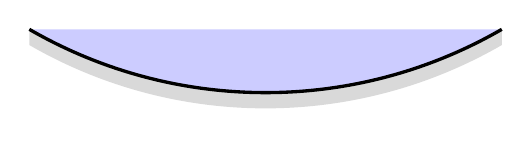
\begin{tikzpicture}
    \fill [fill opacity=0.2, fill=blue] (0,0) arc (240:300:6) -- (0,0) -- cycle;
    \fill [gray!30] (0,0) arc (240:300:6) -- ++(0,-0.2) arc (300:240:6) -- ++(0, 0.2) -- cycle;
    \draw [very thick] (0,0) arc (240:300:6);
  \end{tikzpicture}
\end{figure}
\vspace{-1.5em}
\probend
\bigskip

% Ü163
\setAuthor{Kaarel Hänni}
\setRound{lahtine}
\setYear{2022}
\setNumber{G 9}
\setDifficulty{9}
\setTopic{TODO}

\prob{Nurk}
Spioonil on kodus koer, kellel ta tahab spioneerimise harjutamiseks alati silma peal hoida. Kodus on koridor, mille keskel on nurk suurusega $\alpha$, mille taha vastu seina koer mõnikord konutama läheb. Spioonile meeldib aga konutada teisel pool nurka, samuti vastu seina. Spioonil on selliste puhkude jaoks kumerlääts fookuskaugusega $f=\SI{10}{cm}$, mis on kettakujuline raadiusega $r=\SI{5}{cm}$, mille ta saab asetada koridoris vabalt valitud kohta, vabalt valitud orientatsiooniga. Milline on minimaalne nurk $\alpha$, mille puhul on spioonil võimalik läätse kasutades koera antud situatsioonis jälgida?\\
\emph{Märkus:} võib eeldada, et nii spiooni kui koera kaugus nurgast on palju suuremad kui nende mõõtmed, mis on omakorda palju suuremad kui läätse raadius. Läätse võib vaadelda ideaalse õhukese läätsena.
\probend
\bigskip

% Ü164
\setAuthor{Jaan Kalda}
\setRound{piirkonnavoor}
\setYear{2022}
\setNumber{G 9}
\setDifficulty{9}
\setTopic{TODO}

\prob{Pikne}
Pikselöögi ajal on keskmine voolutugevus $I=\qty{50}{\kA}$ ning selle löögi kestvus
$\tau=\qty{600}{\us}$. Vaakumi dielektriline läbitavus $\varepsilon_0=\qty{8.85e-12}{\F\per\m}$.\\
\osa Hinnake, millise murdosa oma laengust kaotab äikesepilv, kui elektrivälja tugevus enne pikselööki oli maapinna lähedal $E=\qty{20}{\kV\per\m}$.  Äikesepilve diameeter $d=\qty{24}{\km}$. \emph{Vihje}: võite maapinda vaadelda kui plaatkondensaatori alumist plaati ja äikesepilve kui selle ülemist plaati.\\
\osa Pinnase eritakistus on $\rho = \qty{100}{\ohm\m}$. Inimene seisab äikse ajal paljajalu ja jalad harkis ning saab märkimisväärse elektrilöögi, sest jalgadele rakendub pinge $V=\qty{300}{\V}$. Hinnake, kui kaugele inimesest lõi välk maasse.
\probend
\bigskip

% Ü165
\setAuthor{Jaan Kalda}
\setRound{lõppvoor}
\setYear{2022}
\setNumber{G 9}
\setDifficulty{9}
\setTopic{TODO}

\prob{Satelliit}
Millise temperatuuri omandab väike kuubikujuline absoluutselt must satelliit, mis liigub Maa ümber madalal ringorbiidil (kõrgus maapinnast on hulga väiksem, kui Maa raadius) ja on parajasti öö külje peal. \\
Vihje: Maad võib vaadelda kui lõpmatut tasandit, mis on temperatuuril $T_0=\SI{15}\celsius$ ja omab kiirgustegurit $\epsilon=\num{0.6}$, st tema soojuskiirgustihedus ($\SI{}{\watt / \metre\squared}$) on 60\% samasuguse absoluutselt musta keha soojuskiirgustihedusest $\sigma T^4$, kus $\sigma$ tähistab Stefan‐Boltzmanni konstanti.
\probend
\bigskip

% Ü166
\setAuthor{Taavet Kalda}
\setRound{lahtine}
\setYear{2023}
\setNumber{G 9}
\setDifficulty{9}
\setTopic{TODO}

\prob{Klots ja silinder}
\begin{wrapfigure}[8]{r}{0.4\linewidth}
    \vspace{-25pt}
    \begin{center}
        \includegraphics[width=\linewidth]{2023-lahg-09-yl.pdf}
    \end{center}
\end{wrapfigure}
Anul on samasuguse läbimõõdu ja massiga pikk silinder ja klots. Ta lasi silindril mäenõlvast alla veereda ning mõõtis ajaks $t_1 = \SI{5}{\second}$. Seejärel lasi ta klotsil alla libiseda ning sai ajaks $t_2 = \SI{7}{\second}$. Kui palju kuluks silindril ja klotsil mäest alla jõudmiseks, kui need joonisel näidatud moel liigesega ühendada? Võib eeldada, et mäenõlv on ühtlase kaldenurgaga, hõõrdejõud kõikide pindade vahel on konstantne, silinder veereb alati libisemata ning et igas stenaariumis läbisid objektid sama vahemaa. Silindri inertsimoment on $I=mR^2/2$, kus $m$ on silindri mass ja $R$ selle raadius. Õhutakistusega mitte arvestada.









\newcommand{\magnetvali}{
    \begin{tikzpicture}[scale=0.70]
        \draw (-4,0) -- (4,0);
        \draw (0,-4) -- (0,4);

        \draw[thick,->] (0,2) node [anchor = east] {$(0,h)$}
                            -- ++(60:1.6)
                            node [midway, anchor = west] {$\Vec{v}$};
        \draw (0,2) -- ++ (60:1) node [midway, anchor = south east, xshift = 6] {$\alpha$}
            arc (60:90:1);

        \draw (-2,2) circle (0.25) node[above, anchor = south, yshift = 5] {$B_1$};
        \filldraw (-2,2) circle (0.05);
        
        \draw (2,-2) circle (0.25) node[above, anchor = south, yshift = 5] {$B_1$};
        \filldraw (2,-2) circle (0.05);

        \draw (2,2) circle (0.25) node[above, anchor = south, yshift = 5] {$B_2$};
        \draw (2.25,2) -- (1.75,2);
        \draw (2,1.75) -- (2,2.25);

        \draw (-2,-2) circle (0.25) node[above, anchor = south, yshift = 5] {$B_2$};
        \draw (-2.25,-2) -- (-1.75,-2);
        \draw (-2,-1.75) -- (-2,-2.25);
        
    \end{tikzpicture}
} 

\setlength{\columnsep}{20pt}
\probend
\bigskip

% Ü167
\setAuthor{Jaan Kalda}
\setRound{piirkonnavoor}
\setYear{2023}
\setNumber{G 9}
\setDifficulty{9}
\setTopic{TODO}

\prob{Sügav kaev}
Kilplased ehitasid umbes 11 meetri sügavuse pumbakaevu. Lihtsustatult võime nende kaevu vaadelda kui pikka vertikaalset silindrilist toru, mille ülaotsas tekitab pump alarõhu ja imeb seeläbi vett ülespoole. Toru alumine ots on lahtine: vesi saab sealt vabalt nii sisse kui välja voolata. Kilplased proovisid hommikul vett pumbata --- pumpasid ja pumpasid, aga pumbatoru ülemisest otsast jäi veetase ikka umbes meetri kaugusele.  Nad väsisid ära ja läksid puhkama. Peale paaritunnist puhkust tulid tagasi ja proovisid uuesti, aga nüüd jäi  veetase pumbatoru ülemisest otsast veel kaugemale. Mitme sentimeetri võrra jäi veetase teisel katsel madalamaks? On teada, et õhus oli vett nii enne kui pärast $\rho_a=\SI{8}{\g\per\m\cubed}$, aga et õhk oli soojenenud hommikuselt $T_1=\SI{10}{\celsius}$ väärtuseni $T_2=\SI{20}{\celsius}$, siis suhteline õhuniiskus oli vähenenud $r_1=80\%$-lt $r_2=40\%$-ni. Vee tihedus on $\rho_v=\SI{1000}{\kg\per\m\cubed}$ ja molaarmass $\mu=\SI{18}{\g\per\mol}$, gaasikonstant $R=\SI{8.31}{\joule\per\kelvin\per\mol}$, vabalangemise kiirendus $g=\SI{9.8}{\m\per\s\squared}$. Eeldage, et vee temperatuur torus on võrdne õhutemperatuuriga ning õhurõhk päeva jooksul ei muutunud.
\probend
\bigskip

% Ü168
\setAuthor{Jaan Kalda}
\setRound{lõppvoor}
\setYear{2023}
\setNumber{G 9}
\setDifficulty{9}
\setTopic{TODO}

\prob{Staatiline elekter}
A4 formaadis kile kogupindalaga $S= \SI{630}{\square\cm}$ on laetud ühtlase positiivse pindtihedusega staatilise elektriga. Kui see kile asetada vastu  maandatud metallplaati, mille pindala on kile omast hulga suurem, siis \enquote{kleepub} kile vastu plaati ning selleks, et libistada kilet mööda plaati, on vaja rakendada jõudu $F=\SI{0.1}{\N}$ plaadi sihis; hõõrdetegur kile ja plaadi vahel on $\mu=\num{0.5}$. Kile mass on hulga väiksem kui \SI{20}{\g}. Millise pinge omandab kile metallplaadi suhtes, kui see tõmmata plaadilt lahti ning hoida plaadist kaugusel $h=\SI{5}{\cm}$, paralleelselt plaadiga? Elektriline konstant $\varepsilon_0=\SI{8.85e-12}{\F\per\m}$.
\probend
\bigskip

% Ü169
\setAuthor{Uku Andreas Reigo}
\setRound{lahtine}
\setYear{2024}
\setNumber{G 9}
\setDifficulty{9}
\setTopic{TODO}

\prob{Kondensaatorid}
Kaks ruudukujulise plaadiga õhkkondensaatorit on ühendatud jadamisi ning neile on rakendatud alalispinge $U$. Kondensaatorite plaatide küljepikkused on vastavalt $b$ ja $2b$ ning plaatidevaheline kaugus on $d$, kusjuures $d \ll b$. Kahe kondensaatori vaheline kaugus on $b$. Kondensaatoreid läbib plaadiga paralleelse algkiirusega $v_0$ osake laenguga $q$ ja massiga $m$. Milline on osakese nihe kondensaatori telje sihis, kui ta väljub teise kondensaatori piirkonnast? Eeldage, et osake läbib mõlemat kondensaatorit nende plaate puutumata. Raskuskiirenduse ja kondensaatori ääreefektidega arvestama ei pea. \\
\textit{Vihje:} Kondensaatori mahtuvus on $C=\frac{\varepsilon\varepsilon_0S}{d}$.

\begin{center}
\begin{circuitikz}[european]
\ctikzset{bipoles/cuteswitch/thickness=0.5}
\draw
(0,2) to[short] (0,6)
to[short] (2,6)
to[C] (2,4)
to[short, l^= $b$] (3,4)
to[short](4,4)
to[short] (4,4.85);
\draw
(4,5.15) to [short] (4,6)
to[short, l_ = $2b$] (6,6);

\draw
(0,2) to [battery1, l^ = $U$] (6,2)
to [short] (6,6);

\draw[line width = 1]
(3.25,5.15) to [short] (4.75,5.15);
\draw[line width = 1]
(3.25,4.85) to [short] (4.75,4.85);

\draw[-latex, dashed]
(0.25,5) node[below right] {$m,q$} to [short, l^=$v_0$]  (1.25,5) ;

\end{circuitikz}
\end{center}
\probend
\bigskip

% Ü170
\setAuthor{Konstantin Dukatš}
\setRound{piirkonnavoor}
\setYear{2024}
\setNumber{G 9}
\setDifficulty{9}
\setTopic{TODO}

\prob{Laetud kuul}
\begin{wrapfigure}{r}{0.3\textwidth}
  \vspace{-25pt}
  \begin{center}
  \includegraphics[width=\linewidth]{2024-v2g-09-yl.png}
  \vspace{-30pt}
  \end{center}
\end{wrapfigure}



Metallist kuul raadiusega $a$ on maandatud takistuse $R$ kaudu, vt joonist. Kuulile on suunatud lai elektronide (mass $m$, laeng $-e$) voog, kus elektronide kiirus on $v$ ja elektronide arv ruumalaühiku kohta on  $n$. Millise laengu omandab kuul tasakaalulise olukorra saabudes? Elektronide kiirus on nii suur, $v \gg n e^2 a^2 R / m$, et kuulile kogunev laeng ei suuda nende trajektoori märkimisväärselt kõverdada. Arvtihedus $n$ on nii väike, et elektronide tekitatud elektriväljaga võib mitte arvestada. \textit{Vihje:} Kui kuul kannab laengut $Q$, siis tema pinge maapinna suhtes on $\varphi = \frac{Q}{4\pi\varepsilon_0 a}$.
\probend
\bigskip

% Ü171
\setAuthor{Jaan Kalda}
\setRound{lõppvoor}
\setYear{2024}
\setNumber{G 9}
\setDifficulty{9}
\setTopic{TODO}

\prob{Udu}
Kuiva (st ilma igasuguse veeauruta) õhu molaarmass $\mu_a=\SI{28.97}{\g\per\mole}$, vee molaarmass $\mu_v=\SI{18.02}{\g\per\mole}$. Teatud õhurõhu juures on temperatuuril $T_1=\SI{25}\celsius$ kuiva õhu tihedus $\rho_k=\SI{1182.8}{\g\per\m\cubed}$ ning teatud niiske kuid udupiiskadeta õhumassi tihedus $\rho=\SI{1169.3}{\g\per\m\cubed}$. Milline on selle õhumassi tihedus temperatuuril $T_2=\SI{10}\celsius$, kui on teada, et sellel temperatuuril on küllastunud veeauru tihedus $\rho_m=\SI{9.4}{\g\per\m\cubed}$. Eeldage, et kondenseeruvad udupiisad jäävad õhku hõljuma ja et vee tihedus on palju suurem, kui õhu oma.
\probend
\bigskip

% Ü172
\setAuthor{Jaan Kalda}
\setRound{lahtine}
\setYear{2018}
\setNumber{G 10}
\setDifficulty{10}
\setTopic{TODO}

\prob{Pulk}
\begin{wrapfigure}[7]{r}{0.4\textwidth}
	\vspace{-25pt}
	\begin{center}
		\includegraphics[width = 0.4\textwidth]{2018-lahg-10-yl.pdf}
	\end{center}
\end{wrapfigure}

Õhkuvisatud pulga lendu filmiti liikumatu videokaamera abil ja kahe võrdse intervalli tagant võetud kolm kaadrit kopeeriti juuresolevale joonisele (suuremalt lisalehel). On teada, et esimese ja viimase kasutatud kaadri vahele jäänud ajavahemiku jooksul jäi pulga pöördenurk väiksemaks täispöördest. Pulk pöörles joonise tasandis, pulga pikkus oli $L=\SI{1.0}m$ ja kaadri lühem külg on täpselt vertikaalne; raskuskiirendus $g=\SI{9.8}{m/s^2}$. Kui kaugel pulga jämedamast otsast asub selle massikese? Kui pikk oli esimese ja viimase kaadri vaheline ajavahemik?
\probend
\bigskip

% Ü173
\setAuthor{Andres Põldaru}
\setRound{lahtine}
\setYear{2019}
\setNumber{G 10}
\setDifficulty{10}
\setTopic{TODO}

\prob{Lame maa}
Juku lendab lennukiga $h=\SI{10}{km}$ kõrgusel, suunab kaamera optilise peatelje horisondile ja teeb pildi. Seejärel trükib ta pildi 10x10 cm paberile ($L=\SI{10}{cm}$). Kui palju on pildi servas horisont maakera kumeruse tõttu madalamal kui pildi keskel? Võib eeldada, et see suurus on väga väike. Kaamera vaatenurk $2\beta=\SI{50}{\degree}$, Maa raadius $R=\SI{6000}{km}$.
\probend
\bigskip

% Ü174
\setAuthor{}
\setRound{piirkonnavoor}
\setYear{2019}
\setNumber{G 10}
\setDifficulty{10}
\setTopic{TODO}

\prob{3 dioodi}
Joonisel näidatud skeem sisaldab kahte ühesugust takistit ($r=\SI {1.0}\ohm$) ning kolme valgusdioodi: sinist, rohelist ja punast, mis on tähistatud vastavalt tähtedega $S$, $R$ ja $P$. Dioodide voolutugevuse sõltuvuse pingest võib lugeda lihtsuse mõttes selliseks nagu näidatud kõrvaloleval graafikul: voolutugevus on null, kui dioodile rakendatud päripinge on väiksem avanemispingest $V_a$ ning suvalise nullist erineva pärivoolu korral on dioodi pinge võrdne $V_a$-ga. Avanemispinged on dioodidel järgmised: sinisel $\SI{3.2}V$, rohelisel  $\SI{2.6}V$ ja punasel  $\SI{1.8}V$. Sisendklemmidele $A$ ja $B$ rakendatakse konstantse voolu allikas, mis hoiab klemmi $A$ siseneva ning klemmist $B$ väljuva voolu võrdse $I=\SI{1.0}A$-ga. Millist võimsust tarbivad dioodid (näidata ära iga dioodi võimsus eraldi)? 
\includegraphics[scale=0.8]{2019-v2g-10-yl.pdf}
\probend
\bigskip

% Ü175
\setAuthor{}
\setRound{lõppvoor}
\setYear{2019}
\setNumber{G 10}
\setDifficulty{10}
\setTopic{TODO}

\prob{Pöörduv elektriväli}
Elektriväli $\vec E$ muudab perioodiga $4T$ oma suunda pöördudes $x-y$-tasandis iga 
ajavahemiku $T$ möödudes hüppeliselt $\SI{90}\degree$ päripäeva. Seega, kui $t$ tähistab aega 
ning $\hat x$ ja $\hat y$ tähistavad vastavalt $x$- ja $y$-telje sihilisi ühikvektoreid,  siis ajavahemikel
\begin{align*}
4nT\le &t < 4nT+T \;\; & \vec E&=E_0\hat x,\\
4nT+T\le &t < 4nT+2T   & \vec E&=-E_0\hat y,\\
4nT+2T\le &t < 4nT+3T  & \vec E&=-E_0\hat x \;\;\mbox{ja}\\
4nT+3T\le &t < 4nT+4T & \vec E&=E_0\hat y.
\end{align*}

On teada, et osake massiga $m$ ja laenguga $q$ liigub perioodiliselt, st mööda kinnist trajektoori; visandage selle osakese 
trajektoor $x-y$-tasandis ja leidke trajetoori $x$-telje sihiline läbimõõt.
\probend
\bigskip

% Ü176
\setAuthor{Jaan Kalda}
\setRound{lahtine}
\setYear{2020}
\setNumber{G 10}
\setDifficulty{10}
\setTopic{TODO}

\prob{Koonus}
Vabalt painduva venimatu niidi otstes on kuulid massidega $m$ ja $2m$, vt joonist. Kuul massiga $2m$ lebab koonilisel pinnal, mis moodustab horisondiga nurga $\alpha=30^\circ$, raskuskiirendus $g$ on vertikaalselt alla suunatud. Alghetkel on niit pingul ja koonusel lebava kuuli kiirusvektor mooduliga $v_0$ lebab koonuse pinna tasandis moodustades nurga $\beta$ niidiga (st kuuli ja koonuse tippu ühendava sihiga). Teine kuul liigub vertikaalselt niidi pinge ja raskusjõu koosmõjul, algkiirusega $v_0\cos\beta$. Kõiki hõõrdejõude võib ignoreerida.\\
	\osa Kui pika aja pärast  jõuab teine kuul oma teekonna madalaimasse punkti eeldusel, et esimene kuul püsib koonilisel pinnal?\\
	\osa Milline võrratus peab olema rahuldatud, et eelmises punktis tehtud eeldus kehtiks, st et kuulike ei kerkiks kooniliselt pinnalt õhku?
	
	\begin{center}
		\vspace{-13pt}
		\includegraphics[width=0.55\linewidth]{2020-lahg-10-yl.pdf}
	\end{center}
\probend
\bigskip

% Ü177
\setAuthor{}
\setRound{piirkonnavoor}
\setYear{2020}
\setNumber{G 10}
\setDifficulty{10}
\setTopic{TODO}

\prob{Teleskoop}
On antud 4 ühesugust õhukest kumerläätse fookuskaugusega $f$ ning toru pikkusega $12f$ mille siseläbimõõt ühtib läätse välisläbimõõduga. Leidke maksimaalne suurendus teleskoobile mille saab ehitada nendest komponetidest. Lisage optiline skeem. 
\emph{Märkus:} Teleskoop on optiline seade, mille sisenevad ja väljuvad kiired on paralleelsed. Teleskoobi suurenduseks nimetatakse nurksuurendust $ \beta = {\alpha}_{2} / {\alpha}_{1}$, kus $\alpha_1$ on nurk mille all paistab ese vaatleja jaoks ilma teleskoobita ja $\alpha_2$ on nurk mille all paistab eseme kujutis teleskoobis. (Näiteks kahe läätse puhul $ \beta = f_1 / f_2 $.)
\probend
\bigskip

% Ü178
\setAuthor{}
\setRound{lõppvoor}
\setYear{2020}
\setNumber{G 10}
\setDifficulty{10}
\setTopic{TODO}

\prob{Ruut}
\begin{wrapfigure}{r}{0.35\textwidth}
  \vspace{-25pt}
  \begin{center}
  \includegraphics[scale=0.44]{2020-v3g-10-yl.pdf}
  \end{center}
  \vspace{-25pt}
\end{wrapfigure}
Ühtlase takistusega ruudust plaadi vastastippude vaheliseks takistuseks mõõdetakse
$R$, vt joonis (a). Milline tulemus saadakse sama ruudu vastaskülgede keskpunktide
vahelise takistuse mõõtmisel, vt joonis (b)? Mõlemal juhul kasutatakse oommeetri
ühendamiseks samu kettakujulisi tühise takistusega elektroode, mis surutakse vastu
plaati nii nagu näidatud joonisel.
\probend
\bigskip

% Ü179
\setAuthor{Kaarel Kivisalu}
\setRound{lahtine}
\setYear{2021}
\setNumber{G 10}
\setDifficulty{10}
\setTopic{TODO}

\prob{Kolmnurk}
Traadist on tehtud võrdkülgne kolmnurk, mille sisse on pandud lõputult palju samast traadist tehtud võrdkülgseid kolmnurki (vt joonist). Traadi takistus pikkusühiku kohta on selline, et kolmnurga $ABC$ ühe külje takistus on $R$. Leidke kolmnurga $ABC$ tippude $A$ ja $B$ vaheline takistus.

\begin{figure}[h]
  \centering
  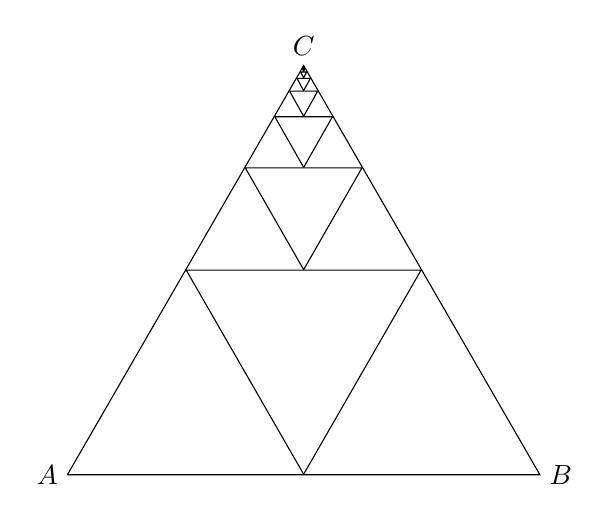
\begin{tikzpicture}[scale=3]
    \draw (0,0) node[left] {$A$} -- (2,0) node[right] {$B$}-- (1, 1.732) node[above] {$C$} -- (0,0);
    \foreach \x in {0,...,7}
    {
      \draw[line cap = round] (1, 1.734-1.732/2^\x) -- (1.003-0.5/2^\x,1.732-0.866/2^\x) -- (0.997+0.5/2^\x,1.732-0.866/2^\x) -- (1, 1.734-1.732/2^\x);
    }
  \end{tikzpicture}
\end{figure}
\probend
\bigskip

% Ü180
\setAuthor{Päivo Simson}
\setRound{piirkonnavoor}
\setYear{2021}
\setNumber{G 10}
\setDifficulty{10}
\setTopic{TODO}

\prob{Laeva vettelaskmine}
Laeva lastakse aeglaselt mööda kaldpinda vette. Selleks, et laev liiga kiiresti ei libiseks, hoitakse seda paigal laeva ninasse kinnitatud tugeva köie abil (vt joonist). Laeva mass on $m$,  kaldpinna kaldenurk horisondi suhtes on $\alpha$ ning hõõrdetegur laeva ja kaldpinna vahel on $\mu$. Leidke laeva paigalhoidmiseks vajalik minimaalne tõmbejõud $T_{min}=|\overrightarrow{T}_{min}|$ köies. Eeldage, et laev veel vett ei puuduta.
\begin{center}
	\includegraphics[width=0.4\linewidth]{2021-v2g-10-yl.pdf}
\end{center}
\probend
\bigskip

% Ü181
\setAuthor{Taavet Kalda}
\setRound{lõppvoor}
\setYear{2021}
\setNumber{G 10}
\setDifficulty{10}
\setTopic{TODO}

\prob{Sirgvool}
Lõputut sirget traati läbib vool $I$. Kaugusel $r$ traadi teljest tulistatakse elektron teatud suunas kiirusega $v_0$. On teada, et edaspidise liikumise käigus on elektroni traadi sihiline kiiruskomponent konstantne. Milline on elektroni trajektoor ning missuguse kiirusega see piki telge liikuma hakkab? Elektroni laengu ja massi suhe on $e/m_e$, vaakumi magnetiline läbitavus on $\mu_0$.
\probend
\bigskip

% Ü182
\setAuthor{Marko Tsengov}
\setRound{lahtine}
\setYear{2022}
\setNumber{G 10}
\setDifficulty{10}
\setTopic{TODO}

\prob{Hantel ja pöörlemine}
\begin{wrapfigure}{r}{0.45\textwidth}
\raisebox{0pt}[\dimexpr\height-0.6\baselineskip\relax]{\includegraphics[scale=0.37]{2022-lahg-10-yl.pdf}}
\vspace{-15pt}
\end{wrapfigure}
Hantel koosneb kahest ühesugusest silindrist raadiusega $r$ ning kõrgusega $d$, mis on ühendatud koaksiaalselt vardaga pikkusega $l$. Varda sees on mootor, mis pöörab silindreid varda suhtes võrdsete ja vastassuunaliste nurkkiirustega $\pm \omega_s$. Millise püsiva nurkkiiruse $\omega_v$ omandab varras, kui hantel asetatakse siledale horisontaalpinnale? Eeldada, et varras ei hakka pöörlema ümber oma telje (nt saab seda takistada kinnitades varda keskkohast alla rippuva lisaraskuse).
\probend
\bigskip

% Ü183
\setAuthor{Jaan Kalda}
\setRound{piirkonnavoor}
\setYear{2022}
\setNumber{G 10}
\setDifficulty{10}
\setTopic{TODO}

\prob{Pingpong}
Juuresoleval graafikul (suuremalt lisalehel) on toodud heli intensiivsus (detsibellides) funktsioonina ajast, kui pingpongipall põrkab üles-alla vastu horisontaalset lauda. Heli tugevuse andmepunktid on võetud ligikaudu iga \num{0.1} sekundi järel. Leidke graafikut kasutades nii täpselt kui võimalik, mitu protsenti palli kineetilisest energiast muundub iga põrke ajal soojuseks\\
\osa esimeste põrgete ja \\
\osa viimaste põrgete jaoks.\\
Pidage silmas, et see protsent püsib enam-vähem konstantne esimesest kuni viienda põrkeni ning samuti alates kolmeteistkümnendast põrkest kuni põrkumiste lõpuni.
\begin{figure}[!h]
  \centering
  \includegraphics[width=\textwidth]{2022-v2g-10-yl.pdf}
\end{figure}
\probend
\bigskip

% Ü184
\setAuthor{Konstantin Dukats}
\setRound{lõppvoor}
\setYear{2022}
\setNumber{G 10}
\setDifficulty{10}
\setTopic{TODO}

\prob{Plaat}
Väike ringikujuline laenguta metallist plaat raadiusega $r$ ja paksusega $h$ asetati plaadi teljel olevast punktlaengust $q$ kaugusele $R$. Hinnake, millise jõuga $F$ tõmbub või tõukub plaat laengu poole. Võite eeldada, et $h\ll r\ll R$ ja plaadi keskme ning ääre juurde indutseeritud laengute tõttu tekkinud jõud on tühiselt väike.
\probend
\bigskip

% Ü185
\setAuthor{Uku Andreas Reigo}
\setRound{lahtine}
\setYear{2023}
\setNumber{G 10}
\setDifficulty{10}
\setTopic{TODO}

\prob{Kõver trajektoor}
\begin{wrapfigure}{r}{0pt}
    \vspace{-50pt}
    \raisebox{-50pt}[0.5\dimexpr\height][-10000pt]{\magnetvali{}}    
    \vspace{-500pt}
\end{wrapfigure}



Elektron massiga $m$ ja laenguga $q$ alustab liikumist punkis $(0,h)$ kiirusega $v$ (vt joonis), kusjuures kiirusvektori ja y-telje sihi vaheline nurk on $\alpha$ nii, et $0<\alpha<\frac{\pi}{4}$. Milline peab olema magnetväljade tugevuste suhe $\frac{B_1}{B_2}$, et elektroni edasine trajektoor oleks kinnine ning ennast mitte lõikav?
\probend
\bigskip

% Ü186
\setAuthor{Jaan Kalda}
\setRound{piirkonnavoor}
\setYear{2023}
\setNumber{G 10}
\setDifficulty{10}
\setTopic{TODO}

\prob{Alajaama kaugus}
Maja peakaitsmeni tuuakse elektrivool alajaamast jämeda alumiiniumist juhtmepaari abil, millest üks, nn nulljuhe, on maandatud alajaama juures. Mõlemad juhtmed on ühepikkused ja ühesuguse ristlõike pindalaga $S=\SI{35}{\mm\squared}$. Alumiiniumi eritakistus on $\rho=\SI{2.7e-8}{\ohm\m}$. Tegemist on elektriliini kõige alajaamapoolsema tarbimispunktiga --- elektriliin jätkub järgmiste majapidamiste poole. Maja sees on elektri edasi kandmiseks peenemad sinist ja pruuni värvi juhtmed, mis on peakaitsmes ühendatud alajaamast tulevate juhtmete külge: sinine on ühendatud nulljuhtmega ja pruun võrgupinget kandva nn faasijuhtmega. Peale selle saab peakaitsme juurest alguse sealsamas maandatud rohe-kollane maandusjuhe. Maandamine tagab selle, et juhe omab maapinna elektrilist potentsiaali (kui juhtmes on elektrivool, siis kehtib see vaid maanduspunkti lähedal; maandusjuhtmes voolu ei ole). Et maapind on hea elektrijuht, siis on maapinna potentsiaal kõikjal üks ja sama. 

Kui majas on sisse lülitud  elektriradiaator, siis on maja peakaitsme juures pinge sinise ja kolla-rohelise juhtme vahel $U_1=\SI{30}\V$  ning sinise ja pruuni vahel $U_f=\SI{210}\V$. Radiaatori nominaalpinge on $U_n=\SI{230}\V$ ja nominaalvõimsus on $P_n=\SI 2{\kW}$ (st kui radiaatorile rakendatakse nominaalpinge, siis eraldub radiaatoril nominaalvõimsus). Radiaatori välja lülitamisel väheneb rohe-kollase juhtme ja sinise juhtme vaheline pinge väärtuseni $U_0=\SI{20}\V$. Kui pikk on majast alajaamani viiv juhtmepaar? Eeldage, et nii radiaatorit kui ka elektriliinil paiknevaid teisi tarbijaid võib heas lähenduses vaadelda kui takisteid. Muuhulgas tähendab see, et kuigi võrgus on vahelduvpinge, võib arvutusi teha täpselt samamoodi nagu alalispinge puhul.
\probend
\bigskip

% Ü187
\setAuthor{Jaan Kalda}
\setRound{lõppvoor}
\setYear{2023}
\setNumber{G 10}
\setDifficulty{10}
\setTopic{TODO}

\prob{Uppuv pall}
Vees ujub vettinud ja vett täis tennisepall nii, et see on peaaegu üleni vee all ning ülemine serv puudutab veepinda. Kaldalt, $H=\SI 2\m$ kõrguselt vaadates näib, et pall on ellipsoidi kujuliselt lapik, kusjuures laiuse ja kõrguse suhe on $k=3$. Kui kaugel vaataja silmast on pall, kui vee murdumisnäitaja $n=\frac 43$? Ülesande lahendamisel võib teha mõistlikke lähendusi.
\probend
\bigskip

% Ü188
\setAuthor{Jaan Kalda}
\setRound{lahtine}
\setYear{2024}
\setNumber{G 10}
\setDifficulty{10}
\setTopic{TODO}

\prob{Pärituul}
Jalgrattur sõidab mööda teed.  Samal ajal puhub pooleldi selja tagant tuul, mille kiirus on täpselt võrdne jalgratturi kiirusega; tuule suund moodustab tee sihiga nurga $\alpha<90^\circ$. Milliste nurga $\alpha$ väärtuste puhul tuul takistab sõitmist (st rattur saaks tuulevaikse ilmaga sama kiiresti sõita kulutades õhutakistuse ületamiseks väiksemat võimsust)? Lugeda, et õhu takistusjõud on võrdeline ratturi kiiruse ruuduga õhu suhtes.
\probend
\bigskip

% Ü189
\setAuthor{Päivo Simson}
\setRound{piirkonnavoor}
\setYear{2024}
\setNumber{G 10}
\setDifficulty{10}
\setTopic{TODO}

\prob{Põrked}
\begin{wrapfigure}{r}{0.25\textwidth}
\vspace{-25pt}
  \begin{center}
    \includegraphics[width=\linewidth]{2024-v2g-10-yl.pdf}
    %\caption{}
  \end{center}
  \vspace{-1cm}
\end{wrapfigure}

Väiksel kummipallil lastakse kukkuda poolkera sisse, mille raadius on $R$. Kõrvaloleval lõikel on näidatud palli algne asukoht, mis on kaugusel $a$ kera tsentrist. Palli algkiirus on null. Leidke üks selline kaugus $a$ ($0<a<R$), mille korral liikumine pärast esimest põrget on perioodiline.
\probend
\bigskip

% Ü190
\setAuthor{Konstantin Dukatš}
\setRound{lõppvoor}
\setYear{2024}
\setNumber{G 10}
\setDifficulty{10}
\setTopic{TODO}

\prob{Kondensaator vedelikus}
\begin{wrapfigure}[9]{r}{3cm}
  \vspace*{-5mm}
  \begin{tikzpicture}
    \colorlet{watercolor}{blue!80!cyan!10!white}
    \tikzstyle{water}=[draw=none, top color=watercolor!90!black!90, bottom color=watercolor!90!black!90, middle color=watercolor!80,shading angle=0]
    \tikzstyle{waterborder}=[draw=blue!50!black]
    \def\l{0.9} % Water height
    \def\L{1.2*\l} % Container height
    \def\W{3} % Container width
    \def\x{0.5} % Capacitor height
    \def\y{2} % Capacitor width
    \def\h{0.6} % Water height in capacitor
    \def\cW{\W} % Circuit width
    \def\cH{0.9*\y} % Circuit height

    % % Circuit
    % \draw(\W/2 + \x/2, \l+\y/2) -- ++(\cW/2 - \x/2, 0) --++ (0, \cH) to[battery1] node[above, pos=0.1]{$V$} ++(-\cW,0) -- ++(0, -\cH) -- (\W/2 - \x/2, \l+\y/2);
    \draw(\W/2 + \x/2, \l+\y/2) -- ++(\cW/2 - \x/2, 0) --++ (0, \cH) --++ (-0.3*\cW, 0) to[open, name=V1, o-o] ++(-0.4*\cW,0) --++ (-0.3*\cW, 0) --++ (0, -\cH) -- (\W/2 - \x/2, \l+\y/2);
    \node  at (V1.center) {$V$};

    % Water
    \draw[water]
    (0,0) -- ++(\W,0) -- ++(0,\l) -- ++(-\W/2 + \x/2,0) -- ++(0,\h) -- ++(-\x,0) -- ++(0,-\h) --  ++(-\W/2+\x/2,0) -- ++(0,-\l);
    \draw[waterborder]
    (0, \l) -- ++(\W/2 - \x/2, 0)
    (\W, \l) -- ++(-\W/2 + \x/2, 0)
    (\W/2 - \x/2, \l + \h) -- ++(\x, 0);

    % Container
    \draw[thick] (0, 0) -- ++(\W,0);

    % Capacitor
    \draw[ultra thick] (\W/2 - \x/2, \l) -- ++(0, \y);
    \draw[ultra thick] (\W/2 + \x/2, \l) -- ++(0, \y);

    % Labels
    \draw[dashed] (\W/2 + \x/2, \l+\h) -- ++(\x,0);
    \draw[latex-latex] (\W/2 + \x, \l) -- ++(0, \h) node[midway,right] {$h$};

    \draw[latex-latex] (\W/2 - \x/2, \l+0.8*\y) -- ++(\x, 0) node[midway,above] {$d$};
  \end{tikzpicture}
\end{wrapfigure}
Plaatkondensaator plaatidevahelise kaugusega $d$ on vertikaalasendis ja otsapidi vedelikus nii, nagu näidatud joonisel. Vedeliku dielektriline läbitavus on $\varepsilon$ ja kondensaatori plaatidele on rakendatud pinge $V$. Kui kõrgel $h$ on  plaatide vahelises ruumiosas vedeliku nivoo võrreldes ülejäänud vaba vedeliku pinnaga? Vaakumi dielektriline läbitavus on $\varepsilon_0$, õhu dielektriline läbitavus $\varepsilon_g=1$, vedeliku tihedus on $\rho$ ja vabalangemise kiirendus on $g$. Vedeliku pindpinevusega võib mitte arvestada; kondensaatori kõrgus ja laius ning õhuga täidetud kondensaatoriosa kõrgus on palju suuremad, kui $d$.
\begin{center}
\end{center}
\probend
\bigskip
\newpage\normalsize\section{Vihjed}
        \toggleHint
        
% V1
\setAuthor{Erkki Tempel}
\setRound{lahtine}
\setYear{2018}
\setNumber{G 1}
\setDifficulty{1}
\setTopic{TODO}

\prob{Kärbes}
\hint

\probend
\bigskip

% V2
\setAuthor{Markus Rene Pae}
\setRound{lahtine}
\setYear{2019}
\setNumber{G 1}
\setDifficulty{1}
\setTopic{TODO}

\prob{Ristmik}
\hint

\probend
\bigskip

% V3
\setAuthor{}
\setRound{piirkonnavoor}
\setYear{2019}
\setNumber{G 1}
\setDifficulty{1}
\setTopic{TODO}

\prob{Rong}
\hint

\probend
\bigskip

% V4
\setAuthor{}
\setRound{lõppvoor}
\setYear{2019}
\setNumber{G 1}
\setDifficulty{1}
\setTopic{TODO}

\prob{Autod}
\hint

\probend
\bigskip

% V5
\setAuthor{Kaarel Kivisalu}
\setRound{lahtine}
\setYear{2020}
\setNumber{G 1}
\setDifficulty{1}
\setTopic{TODO}

\prob{Pudel}
\hint

\probend
\bigskip

% V6
\setAuthor{}
\setRound{piirkonnavoor}
\setYear{2020}
\setNumber{G 1}
\setDifficulty{1}
\setTopic{TODO}

\prob{Saun}
\hint

\probend
\bigskip

% V7
\setAuthor{}
\setRound{lõppvoor}
\setYear{2020}
\setNumber{G 1}
\setDifficulty{1}
\setTopic{TODO}

\prob{Klaaskera}
\hint

\probend
\bigskip

% V8
\setAuthor{Jaan Kalda}
\setRound{lahtine}
\setYear{2021}
\setNumber{G 1}
\setDifficulty{1}
\setTopic{TODO}

\prob{Võrkpall}
\hint

\probend
\bigskip

% V9
\setAuthor{Markus Rene Pae}
\setRound{piirkonnavoor}
\setYear{2021}
\setNumber{G 1}
\setDifficulty{1}
\setTopic{TODO}

\prob{Kuul sfääris}
\hint

\probend
\bigskip

% V10
\setAuthor{Oleg Košik}
\setRound{lõppvoor}
\setYear{2021}
\setNumber{G 1}
\setDifficulty{1}
\setTopic{TODO}

\prob{Lumepall}
\hint

\probend
\bigskip

% V11
\setAuthor{Kaur Aare Saar}
\setRound{lahtine}
\setYear{2022}
\setNumber{G 1}
\setDifficulty{1}
\setTopic{TODO}

\prob{Titicaca järv}
\hint

\probend
\bigskip

% V12
\setAuthor{Richard Luhtaru}
\setRound{piirkonnavoor}
\setYear{2022}
\setNumber{G 1}
\setDifficulty{1}
\setTopic{TODO}

\prob{Peegel peeglis}
\hint

\probend
\bigskip

% V13
\setAuthor{Jaan Kalda}
\setRound{lõppvoor}
\setYear{2022}
\setNumber{G 1}
\setDifficulty{1}
\setTopic{TODO}

\prob{Kettaheide}
\hint

\probend
\bigskip

% V14
\setAuthor{Uku Andreas Reigo}
\setRound{lahtine}
\setYear{2023}
\setNumber{G 1}
\setDifficulty{1}
\setTopic{TODO}

\prob{Paviljon}
\hint

\probend
\bigskip

% V15
\setAuthor{Richard Luhtaru}
\setRound{piirkonnavoor}
\setYear{2023}
\setNumber{G 1}
\setDifficulty{1}
\setTopic{TODO}

\prob{Valgusvihk}
\hint

\probend
\bigskip

% V16
\setAuthor{Jaan Kalda}
\setRound{lõppvoor}
\setYear{2023}
\setNumber{G 1}
\setDifficulty{1}
\setTopic{TODO}

\prob{Sujuv autosõit}
\hint

\probend
\bigskip

% V17
\setAuthor{Jarl Patrick Paide}
\setRound{lahtine}
\setYear{2024}
\setNumber{G 1}
\setDifficulty{1}
\setTopic{TODO}

\prob{Vabasukeldumine}
\hint

\probend
\bigskip

% V18
\setAuthor{Richard Luhtaru}
\setRound{piirkonnavoor}
\setYear{2024}
\setNumber{G 1}
\setDifficulty{1}
\setTopic{TODO}

\prob{Päikesepaneel}
\hint

\probend
\bigskip

% V19
\setAuthor{Hans Daniel Kaimre}
\setRound{lõppvoor}
\setYear{2024}
\setNumber{G 1}
\setDifficulty{1}
\setTopic{TODO}

\prob{Kelgumägi}
\hint

\probend
\bigskip

% V20
\setAuthor{Erkki Tempel}
\setRound{lahtine}
\setYear{2018}
\setNumber{G 2}
\setDifficulty{2}
\setTopic{TODO}

\prob{2018}
\hint

\probend
\bigskip

% V21
\setAuthor{Valter Kiisk}
\setRound{lahtine}
\setYear{2019}
\setNumber{G 2}
\setDifficulty{2}
\setTopic{TODO}

\prob{Pumpjaam}
\hint

\probend
\bigskip

% V22
\setAuthor{}
\setRound{piirkonnavoor}
\setYear{2019}
\setNumber{G 2}
\setDifficulty{2}
\setTopic{TODO}

\prob{Peegel}
\hint

\probend
\bigskip

% V23
\setAuthor{}
\setRound{lõppvoor}
\setYear{2019}
\setNumber{G 2}
\setDifficulty{2}
\setTopic{TODO}

\prob{Saunauks}
\hint

\probend
\bigskip

% V24
\setAuthor{Hannes Kuslap}
\setRound{lahtine}
\setYear{2020}
\setNumber{G 2}
\setDifficulty{2}
\setTopic{TODO}

\prob{Ruut fookuses}
\hint

\probend
\bigskip

% V25
\setAuthor{}
\setRound{piirkonnavoor}
\setYear{2020}
\setNumber{G 2}
\setDifficulty{2}
\setTopic{TODO}

\prob{Karussell}
\hint

\probend
\bigskip

% V26
\setAuthor{}
\setRound{lõppvoor}
\setYear{2020}
\setNumber{G 2}
\setDifficulty{2}
\setTopic{TODO}

\prob{Kohukesed}
\hint

\probend
\bigskip

% V27
\setAuthor{Eero Vaher}
\setRound{lahtine}
\setYear{2021}
\setNumber{G 2}
\setDifficulty{2}
\setTopic{TODO}

\prob{Plokk}
\hint

\probend
\bigskip

% V28
\setAuthor{Kaur Aare Saar}
\setRound{piirkonnavoor}
\setYear{2021}
\setNumber{G 2}
\setDifficulty{2}
\setTopic{TODO}

\prob{Klaaspudel}
\hint

\probend
\bigskip

% V29
\setAuthor{Jarl Patrick Paide}
\setRound{lõppvoor}
\setYear{2021}
\setNumber{G 2}
\setDifficulty{2}
\setTopic{TODO}

\prob{Pudel}
\hint

\probend
\bigskip

% V30
\setAuthor{Joonas Kalda}
\setRound{lahtine}
\setYear{2022}
\setNumber{G 2}
\setDifficulty{2}
\setTopic{TODO}

\prob{Pliiats}
\hint

\probend
\bigskip

% V31
\setAuthor{Jaan Kalda}
\setRound{piirkonnavoor}
\setYear{2022}
\setNumber{G 2}
\setDifficulty{2}
\setTopic{TODO}

\prob{Juhe}
\hint

\probend
\bigskip

% V32
\setAuthor{Moorits Mihkel Muru}
\setRound{lõppvoor}
\setYear{2022}
\setNumber{G 2}
\setDifficulty{2}
\setTopic{TODO}

\prob{Lumeväli}
\hint

\probend
\bigskip

% V33
\setAuthor{Richard Luhtaru}
\setRound{lahtine}
\setYear{2023}
\setNumber{G 2}
\setDifficulty{2}
\setTopic{TODO}

\prob{Kumerpeegel}
\hint

\probend
\bigskip

% V34
\setAuthor{Konstantin Dukatš}
\setRound{piirkonnavoor}
\setYear{2023}
\setNumber{G 2}
\setDifficulty{2}
\setTopic{TODO}

\prob{Otsene kalorimeetria}
\hint

\probend
\bigskip

% V35
\setAuthor{Jaan Kalda}
\setRound{lõppvoor}
\setYear{2023}
\setNumber{G 2}
\setDifficulty{2}
\setTopic{TODO}

\prob{Elektrikarjus}
\hint

\probend
\bigskip

% V36
\setAuthor{Jarl Patrick Paide}
\setRound{lahtine}
\setYear{2024}
\setNumber{G 2}
\setDifficulty{2}
\setTopic{TODO}

\prob{Kaks kera}
\hint

\probend
\bigskip

% V37
\setAuthor{Moorits Mihkel Muru}
\setRound{piirkonnavoor}
\setYear{2024}
\setNumber{G 2}
\setDifficulty{2}
\setTopic{TODO}

\prob{Hajumine}
\hint

\probend
\bigskip

% V38
\setAuthor{Taavi Pungas}
\setRound{lõppvoor}
\setYear{2024}
\setNumber{G 2}
\setDifficulty{2}
\setTopic{TODO}

\prob{Ragulka}
\hint

\probend
\bigskip

% V39
\setAuthor{Jaan Kalda}
\setRound{lahtine}
\setYear{2018}
\setNumber{G 3}
\setDifficulty{3}
\setTopic{TODO}

\prob{Ring}
\hint

\probend
\bigskip

% V40
\setAuthor{Hans Daniel Kaimre}
\setRound{lahtine}
\setYear{2019}
\setNumber{G 3}
\setDifficulty{3}
\setTopic{TODO}

\prob{Lääts}
\hint

\probend
\bigskip

% V41
\setAuthor{}
\setRound{piirkonnavoor}
\setYear{2019}
\setNumber{G 3}
\setDifficulty{3}
\setTopic{TODO}

\prob{Kärbes}
\hint

\probend
\bigskip

% V42
\setAuthor{}
\setRound{lõppvoor}
\setYear{2019}
\setNumber{G 3}
\setDifficulty{3}
\setTopic{TODO}

\prob{Lennuk}
\hint

\probend
\bigskip

% V43
\setAuthor{Hans Daniel Kaimre}
\setRound{lahtine}
\setYear{2020}
\setNumber{G 3}
\setDifficulty{3}
\setTopic{TODO}

\prob{U-klaas}
\hint

\probend
\bigskip

% V44
\setAuthor{}
\setRound{piirkonnavoor}
\setYear{2020}
\setNumber{G 3}
\setDifficulty{3}
\setTopic{TODO}

\prob{Hüppav silinder}
\hint

\probend
\bigskip

% V45
\setAuthor{}
\setRound{lõppvoor}
\setYear{2020}
\setNumber{G 3}
\setDifficulty{3}
\setTopic{TODO}

\prob{Käivitusvool}
\hint

\probend
\bigskip

% V46
\setAuthor{Konstantin Dukatš}
\setRound{lahtine}
\setYear{2021}
\setNumber{G 3}
\setDifficulty{3}
\setTopic{TODO}

\prob{Kumerpeegel}
\hint

\probend
\bigskip

% V47
\setAuthor{Kaarel Hänni}
\setRound{piirkonnavoor}
\setYear{2021}
\setNumber{G 3}
\setDifficulty{3}
\setTopic{TODO}

\prob{Joogid}
\hint

\probend
\bigskip

% V48
\setAuthor{Oleg Košik}
\setRound{lõppvoor}
\setYear{2021}
\setNumber{G 3}
\setDifficulty{3}
\setTopic{TODO}

\prob{Lääts ja ekraan}
\hint

\probend
\bigskip

% V49
\setAuthor{Kaarel Hänni}
\setRound{lahtine}
\setYear{2022}
\setNumber{G 3}
\setDifficulty{3}
\setTopic{TODO}

\prob{Kõnd eskalaatoril}
\hint

\probend
\bigskip

% V50
\setAuthor{Kaarel Kivisalu}
\setRound{piirkonnavoor}
\setYear{2022}
\setNumber{G 3}
\setDifficulty{3}
\setTopic{TODO}

\prob{Liumägi}
\hint

\probend
\bigskip

% V51
\setAuthor{Richard Luhtaru}
\setRound{lõppvoor}
\setYear{2022}
\setNumber{G 3}
\setDifficulty{3}
\setTopic{TODO}

\prob{Silinder}
\hint

\probend
\bigskip

% V52
\setAuthor{Valter Kiisk}
\setRound{lahtine}
\setYear{2023}
\setNumber{G 3}
\setDifficulty{3}
\setTopic{TODO}

\prob{Kummipael}
\hint

\probend
\bigskip

% V53
\setAuthor{Marten Rannut}
\setRound{piirkonnavoor}
\setYear{2023}
\setNumber{G 3}
\setDifficulty{3}
\setTopic{TODO}

\prob{Ökonoomne sõit}
\hint

\probend
\bigskip

% V54
\setAuthor{Aigar Vaigu}
\setRound{lõppvoor}
\setYear{2023}
\setNumber{G 3}
\setDifficulty{3}
\setTopic{TODO}

\prob{Lääts ja kaks peeglit}
\hint

\probend
\bigskip

% V55
\setAuthor{Richard Luhtaru}
\setRound{lahtine}
\setYear{2024}
\setNumber{G 3}
\setDifficulty{3}
\setTopic{TODO}

\prob{Valguskaabel}
\hint

\probend
\bigskip

% V56
\setAuthor{Hans Daniel Kaimre}
\setRound{piirkonnavoor}
\setYear{2024}
\setNumber{G 3}
\setDifficulty{3}
\setTopic{TODO}

\prob{Valgusdioodid}
\hint

\probend
\bigskip

% V57
\setAuthor{Sandra Schumann}
\setRound{lõppvoor}
\setYear{2024}
\setNumber{G 3}
\setDifficulty{3}
\setTopic{TODO}

\prob{Leedid}
\hint

\probend
\bigskip

% V58
\setAuthor{Erkki Tempel}
\setRound{lahtine}
\setYear{2018}
\setNumber{G 4}
\setDifficulty{4}
\setTopic{TODO}

\prob{Kahurid}
\hint

\probend
\bigskip

% V59
\setAuthor{Kaarel Hänni}
\setRound{lahtine}
\setYear{2019}
\setNumber{G 4}
\setDifficulty{4}
\setTopic{TODO}

\prob{Laetud tasand}
\hint

\probend
\bigskip

% V60
\setAuthor{}
\setRound{piirkonnavoor}
\setYear{2019}
\setNumber{G 4}
\setDifficulty{4}
\setTopic{TODO}

\prob{Vaakum}
\hint

\probend
\bigskip

% V61
\setAuthor{}
\setRound{lõppvoor}
\setYear{2019}
\setNumber{G 4}
\setDifficulty{4}
\setTopic{TODO}

\prob{Konveier}
\hint

\probend
\bigskip

% V62
\setAuthor{Richard Luhtaru}
\setRound{lahtine}
\setYear{2020}
\setNumber{G 4}
\setDifficulty{4}
\setTopic{TODO}

\prob{Noova}
\hint

\probend
\bigskip

% V63
\setAuthor{}
\setRound{piirkonnavoor}
\setYear{2020}
\setNumber{G 4}
\setDifficulty{4}
\setTopic{TODO}

\prob{Elektriruut}
\hint

\probend
\bigskip

% V64
\setAuthor{}
\setRound{lõppvoor}
\setYear{2020}
\setNumber{G 4}
\setDifficulty{4}
\setTopic{TODO}

\prob{Tasakaaluliikur}
\hint

\probend
\bigskip

% V65
\setAuthor{Jaan Kalda}
\setRound{lahtine}
\setYear{2021}
\setNumber{G 4}
\setDifficulty{4}
\setTopic{TODO}

\prob{Kuiv õhk}
\hint

\probend
\bigskip

% V66
\setAuthor{Kaido Reivelt}
\setRound{piirkonnavoor}
\setYear{2021}
\setNumber{G 4}
\setDifficulty{4}
\setTopic{TODO}

\prob{Batüskaaf}
\hint

\probend
\bigskip

% V67
\setAuthor{Richar Luhtaru}
\setRound{lõppvoor}
\setYear{2021}
\setNumber{G 4}
\setDifficulty{4}
\setTopic{TODO}

\prob{Sõit jääl}
\hint

\probend
\bigskip

% V68
\setAuthor{Uku Andreas Reigo}
\setRound{lahtine}
\setYear{2022}
\setNumber{G 4}
\setDifficulty{4}
\setTopic{TODO}

\prob{Kuiv jää}
\hint

\probend
\bigskip

% V69
\setAuthor{Jarl Patrick Paide}
\setRound{piirkonnavoor}
\setYear{2022}
\setNumber{G 4}
\setDifficulty{4}
\setTopic{TODO}

\prob{Kaks tuba}
\hint

\probend
\bigskip

% V70
\setAuthor{Erkki Tempel}
\setRound{lõppvoor}
\setYear{2022}
\setNumber{G 4}
\setDifficulty{4}
\setTopic{TODO}

\prob{Läätsede kolmnurk}
\hint

\probend
\bigskip

% V71
\setAuthor{Päivo Simson}
\setRound{lahtine}
\setYear{2023}
\setNumber{G 4}
\setDifficulty{4}
\setTopic{TODO}

\prob{Kondensaatorid}
\hint

\probend
\bigskip

% V72
\setAuthor{Marten Rannut}
\setRound{piirkonnavoor}
\setYear{2023}
\setNumber{G 4}
\setDifficulty{4}
\setTopic{TODO}

\prob{Droon}
\hint

\probend
\bigskip

% V73
\setAuthor{Kaarel Kivisalu}
\setRound{lõppvoor}
\setYear{2023}
\setNumber{G 4}
\setDifficulty{4}
\setTopic{TODO}

\prob{Laev}
\hint

\probend
\bigskip

% V74
\setAuthor{Jonatan Kalmus}
\setRound{lahtine}
\setYear{2024}
\setNumber{G 4}
\setDifficulty{4}
\setTopic{TODO}

\prob{Rongiühendus}
\hint

\probend
\bigskip

% V75
\setAuthor{Jaan Kalda}
\setRound{piirkonnavoor}
\setYear{2024}
\setNumber{G 4}
\setDifficulty{4}
\setTopic{TODO}

\prob{Galileo termomeeter}
\hint

\probend
\bigskip

% V76
\setAuthor{Richard Luhtaru}
\setRound{lõppvoor}
\setYear{2024}
\setNumber{G 4}
\setDifficulty{4}
\setTopic{TODO}

\prob{Piljard}
\hint

\probend
\bigskip

% V77
\setAuthor{Andres Põldaru}
\setRound{lahtine}
\setYear{2018}
\setNumber{G 5}
\setDifficulty{5}
\setTopic{TODO}

\prob{Hiiglane}
\hint

\probend
\bigskip

% V78
\setAuthor{Erkki Tempel}
\setRound{lahtine}
\setYear{2019}
\setNumber{G 5}
\setDifficulty{5}
\setTopic{TODO}

\prob{Kuulid}
\hint

\probend
\bigskip

% V79
\setAuthor{}
\setRound{piirkonnavoor}
\setYear{2019}
\setNumber{G 5}
\setDifficulty{5}
\setTopic{TODO}

\prob{Osake magnetväljas}
\hint

\probend
\bigskip

% V80
\setAuthor{}
\setRound{lõppvoor}
\setYear{2019}
\setNumber{G 5}
\setDifficulty{5}
\setTopic{TODO}

\prob{Jääkeegel}
\hint

\probend
\bigskip

% V81
\setAuthor{Päivo Simson}
\setRound{lahtine}
\setYear{2020}
\setNumber{G 5}
\setDifficulty{5}
\setTopic{TODO}

\prob{Solenoid ja kontuur}
\hint

\probend
\bigskip

% V82
\setAuthor{}
\setRound{piirkonnavoor}
\setYear{2020}
\setNumber{G 5}
\setDifficulty{5}
\setTopic{TODO}

\prob{Purilennuk}
\hint

\probend
\bigskip

% V83
\setAuthor{}
\setRound{lõppvoor}
\setYear{2020}
\setNumber{G 5}
\setDifficulty{5}
\setTopic{TODO}

\prob{Gloobus}
\hint

\probend
\bigskip

% V84
\setAuthor{Jaan Kalda}
\setRound{lahtine}
\setYear{2021}
\setNumber{G 5}
\setDifficulty{5}
\setTopic{TODO}

\prob{Soolvesi}
\hint

\probend
\bigskip

% V85
\setAuthor{Jaan Toots}
\setRound{piirkonnavoor}
\setYear{2021}
\setNumber{G 5}
\setDifficulty{5}
\setTopic{TODO}

\prob{Vooluallikas}
\hint

\probend
\bigskip

% V86
\setAuthor{Kaur Aare Saar}
\setRound{lõppvoor}
\setYear{2021}
\setNumber{G 5}
\setDifficulty{5}
\setTopic{TODO}

\prob{Võimsus}
\hint

\probend
\bigskip

% V87
\setAuthor{Richard Friedrichs}
\setRound{lahtine}
\setYear{2022}
\setNumber{G 5}
\setDifficulty{5}
\setTopic{TODO}

\prob{Originaalsed reostaadid}
\hint

\probend
\bigskip

% V88
\setAuthor{Krister Kasemaa}
\setRound{piirkonnavoor}
\setYear{2022}
\setNumber{G 5}
\setDifficulty{5}
\setTopic{TODO}

\prob{Satelliittelevisioon}
\hint

\probend
\bigskip

% V89
\setAuthor{Valter Kiisk}
\setRound{lõppvoor}
\setYear{2022}
\setNumber{G 5}
\setDifficulty{5}
\setTopic{TODO}

\prob{Jalgratas}
\hint

\probend
\bigskip

% V90
\setAuthor{Valter Kiisk}
\setRound{lahtine}
\setYear{2023}
\setNumber{G 5}
\setDifficulty{5}
\setTopic{TODO}

\prob{Elektriauto}
\hint

\probend
\bigskip

% V91
\setAuthor{Sandra Schumann}
\setRound{piirkonnavoor}
\setYear{2023}
\setNumber{G 5}
\setDifficulty{5}
\setTopic{TODO}

\prob{Vedru keerutamine}
\hint

\probend
\bigskip

% V92
\setAuthor{Kaur Aare Saar}
\setRound{lõppvoor}
\setYear{2023}
\setNumber{G 5}
\setDifficulty{5}
\setTopic{TODO}

\prob{Sundventilatsioon}
\hint

\probend
\bigskip

% V93
\setAuthor{Jaan Kalda}
\setRound{lahtine}
\setYear{2024}
\setNumber{G 5}
\setDifficulty{5}
\setTopic{TODO}

\prob{Värske õhk}
\hint

\probend
\bigskip

% V94
\setAuthor{Marten Rannut}
\setRound{piirkonnavoor}
\setYear{2024}
\setNumber{G 5}
\setDifficulty{5}
\setTopic{TODO}

\prob{Amoksitsilliin}
\hint

\probend
\bigskip

% V95
\setAuthor{Sandra Schumann}
\setRound{lõppvoor}
\setYear{2024}
\setNumber{G 5}
\setDifficulty{5}
\setTopic{TODO}

\prob{Joonlaud koridoris}
\hint

\probend
\bigskip

% V96
\setAuthor{Kaarel Hänni}
\setRound{lahtine}
\setYear{2018}
\setNumber{G 6}
\setDifficulty{6}
\setTopic{TODO}

\prob{Magnetväljad}
\hint

\probend
\bigskip

% V97
\setAuthor{Ardi Loot}
\setRound{lahtine}
\setYear{2019}
\setNumber{G 6}
\setDifficulty{6}
\setTopic{TODO}

\prob{Led}
\hint

\probend
\bigskip

% V98
\setAuthor{}
\setRound{piirkonnavoor}
\setYear{2019}
\setNumber{G 6}
\setDifficulty{6}
\setTopic{TODO}

\prob{Kondensaator}
\hint

\probend
\bigskip

% V99
\setAuthor{}
\setRound{lõppvoor}
\setYear{2019}
\setNumber{G 6}
\setDifficulty{6}
\setTopic{TODO}

\prob{Lõks}
\hint

\probend
\bigskip

% V100
\setAuthor{Taavet Kalda}
\setRound{lahtine}
\setYear{2020}
\setNumber{G 6}
\setDifficulty{6}
\setTopic{TODO}

\prob{Kondensaatorid}
\hint

\probend
\bigskip

% V101
\setAuthor{}
\setRound{piirkonnavoor}
\setYear{2020}
\setNumber{G 6}
\setDifficulty{6}
\setTopic{TODO}

\prob{Kell}
\hint

\probend
\bigskip

% V102
\setAuthor{}
\setRound{lõppvoor}
\setYear{2020}
\setNumber{G 6}
\setDifficulty{6}
\setTopic{TODO}

\prob{Palliviskenõlv}
\hint

\probend
\bigskip

% V103
\setAuthor{Jaan Kalda}
\setRound{lahtine}
\setYear{2021}
\setNumber{G 6}
\setDifficulty{6}
\setTopic{TODO}

\prob{Kaugusvise}
\hint

\probend
\bigskip

% V104
\setAuthor{Jarl Patrick Paide}
\setRound{piirkonnavoor}
\setYear{2021}
\setNumber{G 6}
\setDifficulty{6}
\setTopic{TODO}

\prob{Jalgrattur}
\hint

\probend
\bigskip

% V105
\setAuthor{Krister Kasemaa}
\setRound{lõppvoor}
\setYear{2021}
\setNumber{G 6}
\setDifficulty{6}
\setTopic{TODO}

\prob{Keha keral}
\hint

\probend
\bigskip

% V106
\setAuthor{Jaan Kalda}
\setRound{lahtine}
\setYear{2022}
\setNumber{G 6}
\setDifficulty{6}
\setTopic{TODO}

\prob{Saun}
\hint

\probend
\bigskip

% V107
\setAuthor{Päivo Simson}
\setRound{piirkonnavoor}
\setYear{2022}
\setNumber{G 6}
\setDifficulty{6}
\setTopic{TODO}

\prob{Doomino}
\hint

\probend
\bigskip

% V108
\setAuthor{Jaan Kalda}
\setRound{lõppvoor}
\setYear{2022}
\setNumber{G 6}
\setDifficulty{6}
\setTopic{TODO}

\prob{Õhupüss}
\hint

\probend
\bigskip

% V109
\setAuthor{Marten Rannut}
\setRound{lahtine}
\setYear{2023}
\setNumber{G 6}
\setDifficulty{6}
\setTopic{TODO}

\prob{Võimas mootor}
\hint

\probend
\bigskip

% V110
\setAuthor{Erkki Tempel}
\setRound{piirkonnavoor}
\setYear{2023}
\setNumber{G 6}
\setDifficulty{6}
\setTopic{TODO}

\prob{Klaasplaat}
\hint

\probend
\bigskip

% V111
\setAuthor{Martne Rannut}
\setRound{lõppvoor}
\setYear{2023}
\setNumber{G 6}
\setDifficulty{6}
\setTopic{TODO}

\prob{Nõel vees}
\hint

\probend
\bigskip

% V112
\setAuthor{Jaan Kalda}
\setRound{lahtine}
\setYear{2024}
\setNumber{G 6}
\setDifficulty{6}
\setTopic{TODO}

\prob{Vari}
\hint

\probend
\bigskip

% V113
\setAuthor{Päivo Simson}
\setRound{piirkonnavoor}
\setYear{2024}
\setNumber{G 6}
\setDifficulty{6}
\setTopic{TODO}

\prob{Mitteelastne nöör}
\hint

\probend
\bigskip

% V114
\setAuthor{Uku Andreas Reigo}
\setRound{lõppvoor}
\setYear{2024}
\setNumber{G 6}
\setDifficulty{6}
\setTopic{TODO}

\prob{Jahtumine}
\hint

\probend
\bigskip

% V115
\setAuthor{Krister Kasemaa}
\setRound{lahtine}
\setYear{2018}
\setNumber{G 7}
\setDifficulty{7}
\setTopic{TODO}

\prob{Kauss veega}
\hint

\probend
\bigskip

% V116
\setAuthor{Jaan Kalda}
\setRound{lahtine}
\setYear{2019}
\setNumber{G 7}
\setDifficulty{7}
\setTopic{TODO}

\prob{Niit relssidel}
\hint

\probend
\bigskip

% V117
\setAuthor{}
\setRound{piirkonnavoor}
\setYear{2019}
\setNumber{G 7}
\setDifficulty{7}
\setTopic{TODO}

\prob{Lennurada}
\hint

\probend
\bigskip

% V118
\setAuthor{}
\setRound{lõppvoor}
\setYear{2019}
\setNumber{G 7}
\setDifficulty{7}
\setTopic{TODO}

\prob{3 ruutu}
\hint

\probend
\bigskip

% V119
\setAuthor{Krister Kasemaa}
\setRound{lahtine}
\setYear{2020}
\setNumber{G 7}
\setDifficulty{7}
\setTopic{TODO}

\prob{Poolsilinder basseinis}
\hint

\probend
\bigskip

% V120
\setAuthor{}
\setRound{piirkonnavoor}
\setYear{2020}
\setNumber{G 7}
\setDifficulty{7}
\setTopic{TODO}

\prob{Jälle sauna!}
\hint

\probend
\bigskip

% V121
\setAuthor{}
\setRound{lõppvoor}
\setYear{2020}
\setNumber{G 7}
\setDifficulty{7}
\setTopic{TODO}

\prob{Pulgad}
\hint

\probend
\bigskip

% V122
\setAuthor{Jaan Kalda}
\setRound{lahtine}
\setYear{2021}
\setNumber{G 7}
\setDifficulty{7}
\setTopic{TODO}

\prob{Hantel}
\hint

\probend
\bigskip

% V123
\setAuthor{Kaur Aare Saar}
\setRound{piirkonnavoor}
\setYear{2021}
\setNumber{G 7}
\setDifficulty{7}
\setTopic{TODO}

\prob{Rippuv laeng}
\hint

\probend
\bigskip

% V124
\setAuthor{Jaan Kalda}
\setRound{lõppvoor}
\setYear{2021}
\setNumber{G 7}
\setDifficulty{7}
\setTopic{TODO}

\prob{Kolmnurk}
\hint

\probend
\bigskip

% V125
\setAuthor{Jaan Kalda}
\setRound{lahtine}
\setYear{2022}
\setNumber{G 7}
\setDifficulty{7}
\setTopic{TODO}

\prob{Elektron ja kondensaator}
\hint

\probend
\bigskip

% V126
\setAuthor{Taavet Kalda}
\setRound{piirkonnavoor}
\setYear{2022}
\setNumber{G 7}
\setDifficulty{7}
\setTopic{TODO}

\prob{Plastiliin}
\hint

\probend
\bigskip

% V127
\setAuthor{Oleg Košik}
\setRound{lõppvoor}
\setYear{2022}
\setNumber{G 7}
\setDifficulty{7}
\setTopic{TODO}

\prob{Veeuputus}
\hint

\probend
\bigskip

% V128
\setAuthor{Jaan Kalda}
\setRound{lahtine}
\setYear{2023}
\setNumber{G 7}
\setDifficulty{7}
\setTopic{TODO}

\prob{Soojuspump}
\hint

\probend
\bigskip

% V129
\setAuthor{Päivo Simson}
\setRound{piirkonnavoor}
\setYear{2023}
\setNumber{G 7}
\setDifficulty{7}
\setTopic{TODO}

\prob{Voltmeeter}
\hint

\probend
\bigskip

% V130
\setAuthor{Eero Vaher}
\setRound{lõppvoor}
\setYear{2023}
\setNumber{G 7}
\setDifficulty{7}
\setTopic{TODO}

\prob{Tehiskaaslane}
\hint

\probend
\bigskip

% V131
\setAuthor{Jarl Patrick Paide}
\setRound{lahtine}
\setYear{2024}
\setNumber{G 7}
\setDifficulty{7}
\setTopic{TODO}

\prob{Äikesetorm}
\hint

\probend
\bigskip

% V132
\setAuthor{Jaan Kalda}
\setRound{piirkonnavoor}
\setYear{2024}
\setNumber{G 7}
\setDifficulty{7}
\setTopic{TODO}

\prob{Palgid vees}
\hint

\probend
\bigskip

% V133
\setAuthor{Jaan Kalda}
\setRound{lõppvoor}
\setYear{2024}
\setNumber{G 7}
\setDifficulty{7}
\setTopic{TODO}

\prob{Romb}
\hint

\probend
\bigskip

% V134
\setAuthor{Jaan Kalda}
\setRound{lahtine}
\setYear{2018}
\setNumber{G 8}
\setDifficulty{8}
\setTopic{TODO}

\prob{Kolmnurk}
\hint

\probend
\bigskip

% V135
\setAuthor{Jaan Kalda}
\setRound{lahtine}
\setYear{2019}
\setNumber{G 8}
\setDifficulty{8}
\setTopic{TODO}

\prob{Külm gaas}
\hint

\probend
\bigskip

% V136
\setAuthor{}
\setRound{piirkonnavoor}
\setYear{2019}
\setNumber{G 8}
\setDifficulty{8}
\setTopic{TODO}

\prob{Granaat}
\hint

\probend
\bigskip

% V137
\setAuthor{}
\setRound{lõppvoor}
\setYear{2019}
\setNumber{G 8}
\setDifficulty{8}
\setTopic{TODO}

\prob{Kärbes}
\hint

\probend
\bigskip

% V138
\setAuthor{Jaan Kalda}
\setRound{lahtine}
\setYear{2020}
\setNumber{G 8}
\setDifficulty{8}
\setTopic{TODO}

\prob{Termokaamera}
\hint

\probend
\bigskip

% V139
\setAuthor{}
\setRound{piirkonnavoor}
\setYear{2020}
\setNumber{G 8}
\setDifficulty{8}
\setTopic{TODO}

\prob{Dioodid}
\hint

\probend
\bigskip

% V140
\setAuthor{}
\setRound{lõppvoor}
\setYear{2020}
\setNumber{G 8}
\setDifficulty{8}
\setTopic{TODO}

\prob{Optiline seade}
\hint

\probend
\bigskip

% V141
\setAuthor{Eero Vaher}
\setRound{lahtine}
\setYear{2021}
\setNumber{G 8}
\setDifficulty{8}
\setTopic{TODO}

\prob{Oberthi efekt}
\hint

\probend
\bigskip

% V142
\setAuthor{Hans Daniel Kaimre}
\setRound{piirkonnavoor}
\setYear{2021}
\setNumber{G 8}
\setDifficulty{8}
\setTopic{TODO}

\prob{Lainejuht}
\hint

\probend
\bigskip

% V143
\setAuthor{Taavet Kalda}
\setRound{lõppvoor}
\setYear{2021}
\setNumber{G 8}
\setDifficulty{8}
\setTopic{TODO}

\prob{Veesilinder}
\hint

\probend
\bigskip

% V144
\setAuthor{Päivo Simson}
\setRound{lahtine}
\setYear{2022}
\setNumber{G 8}
\setDifficulty{8}
\setTopic{TODO}

\prob{Kaubalaev}
\hint

\probend
\bigskip

% V145
\setAuthor{Jaan Kalda}
\setRound{piirkonnavoor}
\setYear{2022}
\setNumber{G 8}
\setDifficulty{8}
\setTopic{TODO}

\prob{Tühi pudel}
\hint

\probend
\bigskip

% V146
\setAuthor{Kaur Aare Saar}
\setRound{lõppvoor}
\setYear{2022}
\setNumber{G 8}
\setDifficulty{8}
\setTopic{TODO}

\prob{Veevalaja}
\hint

\probend
\bigskip

% V147
\setAuthor{Valter Kiisk}
\setRound{lahtine}
\setYear{2023}
\setNumber{G 8}
\setDifficulty{8}
\setTopic{TODO}

\prob{Lääts}
\hint

\probend
\bigskip

% V148
\setAuthor{Marko Tsengov}
\setRound{piirkonnavoor}
\setYear{2023}
\setNumber{G 8}
\setDifficulty{8}
\setTopic{TODO}

\prob{Süvend ja kera}
\hint

\probend
\bigskip

% V149
\setAuthor{Valter Kiisk}
\setRound{lõppvoor}
\setYear{2023}
\setNumber{G 8}
\setDifficulty{8}
\setTopic{TODO}

\prob{Kuulitõuge}
\hint

\probend
\bigskip

% V150
\setAuthor{Jaan Kalda}
\setRound{lahtine}
\setYear{2024}
\setNumber{G 8}
\setDifficulty{8}
\setTopic{TODO}

\prob{Käru}
\hint

\probend
\bigskip

% V151
\setAuthor{Hannes Kuslap}
\setRound{piirkonnavoor}
\setYear{2024}
\setNumber{G 8}
\setDifficulty{8}
\setTopic{TODO}

\prob{Hermeetiline saun}
\hint

\probend
\bigskip

% V152
\setAuthor{Jaan Kalda}
\setRound{lõppvoor}
\setYear{2024}
\setNumber{G 8}
\setDifficulty{8}
\setTopic{TODO}

\prob{Kolmnurk}
\hint

\probend
\bigskip

% V153
\setAuthor{Jaan Kalda}
\setRound{lahtine}
\setYear{2018}
\setNumber{G 9}
\setDifficulty{9}
\setTopic{TODO}

\prob{Õhkjahutus}
\hint

\probend
\bigskip

% V154
\setAuthor{Jaan Kalda}
\setRound{lahtine}
\setYear{2019}
\setNumber{G 9}
\setDifficulty{9}
\setTopic{TODO}

\prob{Hantel}
\hint

\probend
\bigskip

% V155
\setAuthor{}
\setRound{piirkonnavoor}
\setYear{2019}
\setNumber{G 9}
\setDifficulty{9}
\setTopic{TODO}

\prob{Kiik}
\hint

\probend
\bigskip

% V156
\setAuthor{}
\setRound{lõppvoor}
\setYear{2019}
\setNumber{G 9}
\setDifficulty{9}
\setTopic{TODO}

\prob{Niit ja poolsfäär}
\hint

\probend
\bigskip

% V157
\setAuthor{Erik Tamre}
\setRound{lahtine}
\setYear{2020}
\setNumber{G 9}
\setDifficulty{9}
\setTopic{TODO}

\prob{Suvi}
\hint

\probend
\bigskip

% V158
\setAuthor{}
\setRound{piirkonnavoor}
\setYear{2020}
\setNumber{G 9}
\setDifficulty{9}
\setTopic{TODO}

\prob{Laengud magnetväljas}
\hint

\probend
\bigskip

% V159
\setAuthor{}
\setRound{lõppvoor}
\setYear{2020}
\setNumber{G 9}
\setDifficulty{9}
\setTopic{TODO}

\prob{Õhupallid}
\hint

\probend
\bigskip

% V160
\setAuthor{Kaarel Hänni}
\setRound{lahtine}
\setYear{2021}
\setNumber{G 9}
\setDifficulty{9}
\setTopic{TODO}

\prob{Pidurdav jalgratas}
\hint

\probend
\bigskip

% V161
\setAuthor{Jaan Kalda}
\setRound{piirkonnavoor}
\setYear{2021}
\setNumber{G 9}
\setDifficulty{9}
\setTopic{TODO}

\prob{Kiiruse kujutis}
\hint

\probend
\bigskip

% V162
\setAuthor{Konstantis Dukatš}
\setRound{lõppvoor}
\setYear{2021}
\setNumber{G 9}
\setDifficulty{9}
\setTopic{TODO}

\prob{Vedelik peeglil}
\hint

\probend
\bigskip

% V163
\setAuthor{Kaarel Hänni}
\setRound{lahtine}
\setYear{2022}
\setNumber{G 9}
\setDifficulty{9}
\setTopic{TODO}

\prob{Nurk}
\hint

\probend
\bigskip

% V164
\setAuthor{Jaan Kalda}
\setRound{piirkonnavoor}
\setYear{2022}
\setNumber{G 9}
\setDifficulty{9}
\setTopic{TODO}

\prob{Pikne}
\hint

\probend
\bigskip

% V165
\setAuthor{Jaan Kalda}
\setRound{lõppvoor}
\setYear{2022}
\setNumber{G 9}
\setDifficulty{9}
\setTopic{TODO}

\prob{Satelliit}
\hint

\probend
\bigskip

% V166
\setAuthor{Taavet Kalda}
\setRound{lahtine}
\setYear{2023}
\setNumber{G 9}
\setDifficulty{9}
\setTopic{TODO}

\prob{Klots ja silinder}
\hint

\probend
\bigskip

% V167
\setAuthor{Jaan Kalda}
\setRound{piirkonnavoor}
\setYear{2023}
\setNumber{G 9}
\setDifficulty{9}
\setTopic{TODO}

\prob{Sügav kaev}
\hint

\probend
\bigskip

% V168
\setAuthor{Jaan Kalda}
\setRound{lõppvoor}
\setYear{2023}
\setNumber{G 9}
\setDifficulty{9}
\setTopic{TODO}

\prob{Staatiline elekter}
\hint

\probend
\bigskip

% V169
\setAuthor{Uku Andreas Reigo}
\setRound{lahtine}
\setYear{2024}
\setNumber{G 9}
\setDifficulty{9}
\setTopic{TODO}

\prob{Kondensaatorid}
\hint

\probend
\bigskip

% V170
\setAuthor{Konstantin Dukatš}
\setRound{piirkonnavoor}
\setYear{2024}
\setNumber{G 9}
\setDifficulty{9}
\setTopic{TODO}

\prob{Laetud kuul}
\hint

\probend
\bigskip

% V171
\setAuthor{Jaan Kalda}
\setRound{lõppvoor}
\setYear{2024}
\setNumber{G 9}
\setDifficulty{9}
\setTopic{TODO}

\prob{Udu}
\hint

\probend
\bigskip

% V172
\setAuthor{Jaan Kalda}
\setRound{lahtine}
\setYear{2018}
\setNumber{G 10}
\setDifficulty{10}
\setTopic{TODO}

\prob{Pulk}
\hint

\probend
\bigskip

% V173
\setAuthor{Andres Põldaru}
\setRound{lahtine}
\setYear{2019}
\setNumber{G 10}
\setDifficulty{10}
\setTopic{TODO}

\prob{Lame maa}
\hint

\probend
\bigskip

% V174
\setAuthor{}
\setRound{piirkonnavoor}
\setYear{2019}
\setNumber{G 10}
\setDifficulty{10}
\setTopic{TODO}

\prob{3 dioodi}
\hint

\probend
\bigskip

% V175
\setAuthor{}
\setRound{lõppvoor}
\setYear{2019}
\setNumber{G 10}
\setDifficulty{10}
\setTopic{TODO}

\prob{Pöörduv elektriväli}
\hint

\probend
\bigskip

% V176
\setAuthor{Jaan Kalda}
\setRound{lahtine}
\setYear{2020}
\setNumber{G 10}
\setDifficulty{10}
\setTopic{TODO}

\prob{Koonus}
\hint

\probend
\bigskip

% V177
\setAuthor{}
\setRound{piirkonnavoor}
\setYear{2020}
\setNumber{G 10}
\setDifficulty{10}
\setTopic{TODO}

\prob{Teleskoop}
\hint

\probend
\bigskip

% V178
\setAuthor{}
\setRound{lõppvoor}
\setYear{2020}
\setNumber{G 10}
\setDifficulty{10}
\setTopic{TODO}

\prob{Ruut}
\hint

\probend
\bigskip

% V179
\setAuthor{Kaarel Kivisalu}
\setRound{lahtine}
\setYear{2021}
\setNumber{G 10}
\setDifficulty{10}
\setTopic{TODO}

\prob{Kolmnurk}
\hint

\probend
\bigskip

% V180
\setAuthor{Päivo Simson}
\setRound{piirkonnavoor}
\setYear{2021}
\setNumber{G 10}
\setDifficulty{10}
\setTopic{TODO}

\prob{Laeva vettelaskmine}
\hint

\probend
\bigskip

% V181
\setAuthor{Taavet Kalda}
\setRound{lõppvoor}
\setYear{2021}
\setNumber{G 10}
\setDifficulty{10}
\setTopic{TODO}

\prob{Sirgvool}
\hint

\probend
\bigskip

% V182
\setAuthor{Marko Tsengov}
\setRound{lahtine}
\setYear{2022}
\setNumber{G 10}
\setDifficulty{10}
\setTopic{TODO}

\prob{Hantel ja pöörlemine}
\hint

\probend
\bigskip

% V183
\setAuthor{Jaan Kalda}
\setRound{piirkonnavoor}
\setYear{2022}
\setNumber{G 10}
\setDifficulty{10}
\setTopic{TODO}

\prob{Pingpong}
\hint

\probend
\bigskip

% V184
\setAuthor{Konstantin Dukats}
\setRound{lõppvoor}
\setYear{2022}
\setNumber{G 10}
\setDifficulty{10}
\setTopic{TODO}

\prob{Plaat}
\hint

\probend
\bigskip

% V185
\setAuthor{Uku Andreas Reigo}
\setRound{lahtine}
\setYear{2023}
\setNumber{G 10}
\setDifficulty{10}
\setTopic{TODO}

\prob{Kõver trajektoor}
\hint

\probend
\bigskip

% V186
\setAuthor{Jaan Kalda}
\setRound{piirkonnavoor}
\setYear{2023}
\setNumber{G 10}
\setDifficulty{10}
\setTopic{TODO}

\prob{Alajaama kaugus}
\hint

\probend
\bigskip

% V187
\setAuthor{Jaan Kalda}
\setRound{lõppvoor}
\setYear{2023}
\setNumber{G 10}
\setDifficulty{10}
\setTopic{TODO}

\prob{Uppuv pall}
\hint

\probend
\bigskip

% V188
\setAuthor{Jaan Kalda}
\setRound{lahtine}
\setYear{2024}
\setNumber{G 10}
\setDifficulty{10}
\setTopic{TODO}

\prob{Pärituul}
\hint

\probend
\bigskip

% V189
\setAuthor{Päivo Simson}
\setRound{piirkonnavoor}
\setYear{2024}
\setNumber{G 10}
\setDifficulty{10}
\setTopic{TODO}

\prob{Põrked}
\hint

\probend
\bigskip

% V190
\setAuthor{Konstantin Dukatš}
\setRound{lõppvoor}
\setYear{2024}
\setNumber{G 10}
\setDifficulty{10}
\setTopic{TODO}

\prob{Kondensaator vedelikus}
\hint

\probend
\bigskip
\newpage\section{Lahendused}
        \toggleSolution
        
% L1
\setAuthor{Erkki Tempel}
\setRound{lahtine}
\setYear{2018}
\setNumber{G 1}
\setDifficulty{1}
\setTopic{TODO}

\prob{Kärbes}
\solu
Minimaalne kaugus on siis, kui kärbes läbib optilist peatelge. Kärbes ja tema kujutis on sel hetkel läätsest kahekordse fookuskauguse kaugusel. Kuna nii kärbes kui ka tema kujutis on läätsest sama kaugel, on kujutise suurendus $1$, mistõttu kujutise liikumiskiirus on sama, mis kärbse liikumiskiirus, ehk $u = v = \SI{0,5}{m/s}$.
\probend
\bigskip

% L2
\setAuthor{Markus Rene Pae}
\setRound{lahtine}
\setYear{2019}
\setNumber{G 1}
\setDifficulty{1}
\setTopic{TODO}

\prob{Ristmik}
\solu
Kui Juku ja teise auto projitseeritu kaugus ristmikust ja kiirused on samad, siis nad jõuavad ristmikule täpselt sama ajaga $t = s/v = \SI{150}{\meter} / \SI{90}{\kilo\meter\per\hour} = \SI{150}{\meter} / \SI{25}{\meter\per\second} = \SI{6}{\second}$. Kui Juku saavuitaks hetkeliselt kiirenduse $a = \SI{0.5}{\meter\per\second\squared}$, siis selle ajaga jõuaks ta läbida $s = v_0 t + a t^2/2 = \SI{25}{\meter\per\second} \cdot \SI{6}{\second} + \SI{0.5}{\meter\per\second\squared} (\SI{6}{\second})^2 / 2 = \SI{159}{\meter}$. Seega on teise auto ristmikule jõudes autode vahemaa $\SI{9}{\meter}$. Nurk ei oma antud ülesandes tähtsust.
\probend
\bigskip

% L3
\setAuthor{}
\setRound{piirkonnavoor}
\setYear{2019}
\setNumber{G 1}
\setDifficulty{1}
\setTopic{TODO}

\prob{Rong}
\solu
Olgu rongi kiirendus $a$. Kuna vagunid on identsed, siis ühe vaguni pikkus $s=\frac{at^2}{2}$. \pp{1} Olgu rongis $n$ vagunit, siis kõik vagunid mööduvad Jukust 
aja $t_n=\sqrt{\frac{2sn}{a}}$ jooksul. \pp{1} Kõik peale viimase vaguni mööduvad aja $t_{n-1}=\sqrt{\frac{2s(n-1)}{a}}$ jooksul. \pp{1} Seega 
$$t_2=t_n-t_{n-1}=\sqrt{\frac{2sn}{a}}-\sqrt{\frac{2s(n-1)}{a}}=t(\sqrt{n}-\sqrt{n-1}) \quad \pp{1}$$
Siit tuleb ruutvõrrand, mille lahendades saame:
$$n = \frac{1}{4}\bigg(\frac{t_2}{t}\bigg)^2 + \frac{1}{2} + \bigg(\frac{t}{4t_2}\bigg)^2 = 7.97 \approx 8 \quad \pp{1}$$
Üle kontrollides ainuke antud vahemikku sobiv $n=8$ \pp{1}.
\probend
\bigskip

% L4
\setAuthor{}
\setRound{lõppvoor}
\setYear{2019}
\setNumber{G 1}
\setDifficulty{1}
\setTopic{TODO}

\prob{Autod}
\solu
Kuna autod jäävad seisma samaaegselt, siis läheme ühe ühe autoga seotud taustsüsteemi.
Autode suhteline kiirus üksteise suhtes on $v = v_1+v_2 = \SI{180}{km/h}=\SI{50}{m/s}$\\
Autode pidurdusteekond on kokku $2=\SI{600}{m}$ ning lõppkiirus on $\SI{0}{m/s}$, siis pidurdamiseks kulunud aeg on
\[ s = \frac{v + v_0}{2}\cdot t \quad\quad\Rightarrow\quad\quad t = \frac{2s}{v+v_0} = \SI{24}{s} \]
\probend
\bigskip

% L5
\setAuthor{Kaarel Kivisalu}
\setRound{lahtine}
\setYear{2020}
\setNumber{G 1}
\setDifficulty{1}
\setTopic{TODO}

\prob{Pudel}
\solu
Olgu algne vee ruumala pudelis $V_0$. Selleks, et ära joodud vee ruumala maksimeerida, peaks ilmselt lõpus pudelit ainult õhk täitma. Vastasel korral on võimalik algset vee ruumala vähendada ning suurema õhu osakaalu arvelt rohkem vett ära juua.

Pudelist joomine on isotermiline protsess. Seega,
\[
p_0 (V-V_0)=(p_0-\Delta p)V.
\]
Siit avaldades $V_0$ saame, et
\[
V_0=\frac{\Delta P}{p_0} V = \num{0.25} V.
\]
\probend
\bigskip

% L6
\setAuthor{}
\setRound{piirkonnavoor}
\setYear{2020}
\setNumber{G 1}
\setDifficulty{1}
\setTopic{TODO}

\prob{Saun}
\solu
Vee mass on $m=\rho V$ ja seega vee soojendamiseks ja aurustumiseks kuluv soojushulk on
$$Q=c_v\rho V (T_k-T_0) + L\rho V, \qquad\pp{1}$$
kus $T_k = \SI{100}{\celsius}$ on keemistemperatuur ja $T_0$ on vee algtemperatuur.

Kui kerise temperatuur väheneb $\Delta T$ võrra ($\Delta T$ on temperatuuri muutuse absoluutväärtus), siis kerise poolt antud soojushulk on
$$Q=c_kM\Delta T \qquad \pp{1}$$
Võrdustades seosed saame
$$\Delta T = \frac{\rho V\left(c_v(T_k-T_0)+L\right)}{c_kM} \qquad\pp{1}$$
Asendades sisse antud väärtused, saame
$$\Delta T_{\text{(külm)}}\approx \SI{7.65}{\celsius} \qquad\pp{1}$$
$$\Delta T_{\text{(kuum)}}\approx \SI{6.81}{\celsius} \qquad\pp{1}$$
Kuna $\frac{\num{7.65}-\num{6.81}}{\num{6.81}}\approx \num{0.12}$ \pp{0,5} on suurem kui 10\%, siis Juhanil ei ole õigus. \pp{0,5}

\emph{Märkus.} Viimases reas lugeda õigeks ka lahendus, mis leiab $\frac{\num{7.65}-\num{6.81}}{\num{6.81}}$ asemel $\frac{\num{7.65}-\num{6.81}}{\num{7.65}}$ väärtuse või leiab, et $\frac{\num{7.65}}{\num{6.81}}>\num{1.1}$.
\probend
\bigskip

% L7
\setAuthor{}
\setRound{lõppvoor}
\setYear{2020}
\setNumber{G 1}
\setDifficulty{1}
\setTopic{TODO}

\prob{Klaaskera}
\solu
Mööda optilist peatelge liikuv kiir ei murdu ning liigub otse läbi kera. Seega koonduvad kõik kiired kera tagumise poole ja optilise peatelje lõikumiskohta. Uurime nüüd üht valguskiirt, mis asub vihu tsentrist eemal. Selle konkreetse valguskiire jaoks võib lähendada probleemi kahedimensionaalseks. Joonistame kiire käigu, märgime nurgad. Langemisnurk olgu $\alpha$ ning murdumisnurk $\beta$, kusjuures need on omavahel seotud Snelli seadusega: $n_{õ}\sin\alpha=n_{k}\sin\beta$. Sarnaste kolmnurkade tõttu $\angle AOB$ on samuti $\alpha$. Kolmnurk $AFO$ on võrdhaarne (haaradeks kera raadiused) ning seega $\angle AFO$ on $\beta$. Ühelt poolt (kolmnurga sisenurkade summa on $180^\circ$) $\angle AOF=180-2\beta$, teisalt (kõrvunurkade summa on $180^\circ$) $\angle AOF=180^\circ-\alpha$, seega $\alpha=2\beta$. Võttes, et $n_{õ}=1$ ning tehes väikeste nurkade lähenduse $\sin x \approx x$, saame:
$$n_{õ}\sin\alpha=n_{k}\sin\beta \Rightarrow \sin2\beta=n_{k}\sin\beta \Rightarrow n_k = \frac{\sin2\beta}{\sin\beta}\approx\frac{2\beta}{\beta}=2.$$
\begin{figure}[htbp!]
\centering
\includegraphics[width=0.6\textwidth]{2020-v3g-01-yl.pdf}
\end{figure}
\probend
\bigskip

% L8
\setAuthor{Jaan Kalda}
\setRound{lahtine}
\setYear{2021}
\setNumber{G 1}
\setDifficulty{1}
\setTopic{TODO}

\prob{Võrkpall}
\solu
Ideaalse gaasi olekuvõrrandi saab uue pallirõhu $p_1$ abil kirjutada kujul $p_1+p_a=(p_0+p_a)T_1/T_0$, kus alg- ja lõpptemperatuurid on kelvinites. Siit saame $p_1=(p_0+p_a)T_1/T_0-p_0\approx \SI{42}{kPa}$, st pall on nüüd liiga suure rõhu all.
\probend
\bigskip

% L9
\setAuthor{Markus Rene Pae}
\setRound{piirkonnavoor}
\setYear{2021}
\setNumber{G 1}
\setDifficulty{1}
\setTopic{TODO}

\prob{Kuul sfääris}
\solu
Läheme pöörlevasse taustsüsteemi. Siis mõjub kuulile kolm jõudu, raskusjõud, tsentrifugaaljõud ja toereaktsioon. Nende jõudude summa peab olema 0, sest pöörlevas taustsüsteemis seisab kuulike paigal. Sfääri pinna ja kuuli vahel puudub hõõrdejõud, seega on kuuli raskusjõu ning tsentrifugaaljõu summavektor sfääri raadiuse sihiline~\pp{1}.\par
Olgu $r$ kuulikese kaugus pöörlemisteljest. Sarnaste kolmnurkade tõttu, suhtuvad raskusjõu ja tsentrifugaaljõu teineteisesse kui $R-h$ ja $r$~\pp{1}. Seega peab kehtima seos:
$$ \frac{mg}{R-h} = \frac{m \omega^2 r}{r} \quad \pp2$$
kus $\omega$ on kuulikese ringsagedus. Viimase avaldise lihtsustamine ning sellest nurkkiiruse $\omega$ avaldamine annab:
$$ \omega = \sqrt{\frac{g}{R-h}} \quad \pp2$$
Kuna $\omega = \frac{2\pi}{T}$ \pp{1}, siis järelikult peab tiirlemise periood olema $T = 2 \pi \sqrt{\frac{R-h}{g}} \approx \SI{1.28}{\second}$ \pp{1}.

\begin{figure}[H]
	\centering
	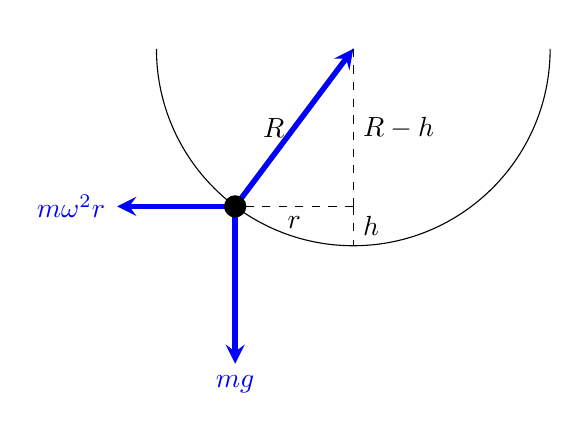
\begin{tikzpicture}[scale=0.5]
    \coordinate (A) at (-5,0);
    \coordinate (O) at (0,0);
    \coordinate (kuul) at (-3,-4);
    \coordinate (base) at (0,-5);
    \coordinate (X) at (0,-4);

    % kauss
    \draw (A) arc (0:180:-5);

    % jooned
    \draw [dashed] (O) -- (0,-4) node[midway,right] {$R-h$};
    \draw (O) -- (-3,-4) node[midway,above,left] {$R$};
    \draw [dashed] (0,-4) -- (base) node[midway,right] {$h$};
    \draw [dashed] (O) -- (kuul);
    \draw [dashed] (X) -- (kuul) node[midway,below] {$r$};

    % jõud
    \draw[line width=2pt,blue,-stealth](kuul)--(-3,-8) node[anchor=north]{$mg$};
    \draw[line width=2pt,blue,-stealth](kuul)--(-6,-4) node[anchor=east]{$m\omega^2r$};
    \draw[line width=2pt,blue,-stealth](kuul)--(O) node[anchor=south west]{};

    % kuul
    \node[circle,fill=black,inner sep=1mm] at (kuul) {};
  \end{tikzpicture}
\end{figure}
\probend
\bigskip

% L10
\setAuthor{Oleg Košik}
\setRound{lõppvoor}
\setYear{2021}
\setNumber{G 1}
\setDifficulty{1}
\setTopic{TODO}

\prob{Lumepall}
\solu
Lumepall peab läbima kiirendusega $g$ vertikaalse teepikkuse $H-h$, seega saame võrduse
$$H-h=\frac{gt^2}{2},$$ kus $t$ on lumepalli lennuaeg. Olgu $w$ lumepalli algkiirus, siis tema horisontaalsuunaline kiirus läheneva Richardi suhtes on $v+w$. Peab kehtima võrdus $$(v+w)t=l.$$ Avaldades esimesest võrdusest $t$ ja teisest $w$ leiame
$$w=l\sqrt{\frac{g}{2(H-h)}}-v\approx \SI{4,7}{m/s}.$$
\probend
\bigskip

% L11
\setAuthor{Kaur Aare Saar}
\setRound{lahtine}
\setYear{2022}
\setNumber{G 1}
\setDifficulty{1}
\setTopic{TODO}

\prob{Titicaca järv}
\solu
Kuna järv on tasakaalus, siis sissetulev vee kogus peab olema võrdne väljamineva vee kogusega.
Vett aurab kiirusega 
\begin{gather*}
v_a = \frac{A \cdot v} {\SI{1}{\aasta}} = \frac{8400 \cdot 2000}{1} \si{\kilo\meter\squared\milli\meter\per \aasta} =
\frac{8400 \cdot 2000 \cdot 1000000 \cdot 0.001}{3600 \cdot 24 \cdot 365.25} \si{\meter\cubed\per\second} = \SI{532}{\meter\cubed\per\second}.
\end{gather*}
Järelikult voolab vett sisse kiirusega $v_s=v + v_a = \SI{542}{\meter\cubed\per\second}$.

Kuna järv on tasakaalus, siis sissetulev soola kogus peab olema võrdne välja mineva soola kogusega. Sisse tuleb soola kiirusega $v_{\text{sool}} = c \cdot v_s  = c_{\text{välja}} \cdot v$.

Järelikult $c_{\text{välja}} = c \frac{v_s}{v} = 10 \frac{542}{10} \si{\milli\gram\per\liter} = \SI{542}{\milli\gram\per\liter}$.
\probend
\bigskip

% L12
\setAuthor{Richard Luhtaru}
\setRound{piirkonnavoor}
\setYear{2022}
\setNumber{G 1}
\setDifficulty{1}
\setTopic{TODO}

\prob{Peegel peeglis}
\solu
Konstrueerime Arvo kujutise peeglis 1 ($A'$), peeglis 2 ($A''$) ja punkti $A'$ kujutise peeglis 2 ($A'''$). Breti nägemiseks on kaks võimalust. Esimene võimalus on ainult peegli 1 kaudu, kiirte käigu saame konstrueerida lõigu $A'B$ abil. Teine võimalus on peegli 1 ja seejärel peegli 2 kaudu, kiirte käigu saame konstrueerida lõigu $A'''B$ abil. Ainult peeglist 2 pole võimalik Bretti näha, sest $A''B$ ei lõiku peegliga 2. Samuti pole peeglist 2 võimalik näha peeglit 1, seega rohkem võimalusi pole.

\begin{figure}[h]
    \centering
    \includegraphics[width=\textwidth, trim=0 50 0 50, clip]{2022-v2g-01-yl.pdf}
\end{figure}
\probend
\bigskip

% L13
\setAuthor{Jaan Kalda}
\setRound{lõppvoor}
\setYear{2022}
\setNumber{G 1}
\setDifficulty{1}
\setTopic{TODO}

\prob{Kettaheide}
\solu
\

\begin{figure}[h]
    \centering
    \includegraphics[]{2022-v3g-01-yl.pdf}
\end{figure}

Jõudiagramm on toodud joonisel. Vastutuul suurendab nii takistusjõudu kui õhuvoolust tingitud üleslükkejõudu. Üleslükkejõud kasvab proportsionaalselt ketta kiirusega õhu suhtes. Suurem üleslükkejõud pikendab lennuaega, mille tulemusel jõuab ketas liikuda horisontaalsihis kaugemale vaatamata sellele, et horisontaalsuunaline kiirus natuke väheneb takistusjõu tõttu (esimene efekt on tugevam, kui teine).
\probend
\bigskip

% L14
\setAuthor{Uku Andreas Reigo}
\setRound{lahtine}
\setYear{2023}
\setNumber{G 1}
\setDifficulty{1}
\setTopic{TODO}

\prob{Paviljon}
\solu
Mõistame, et ülesande tingimustest tuletatav piiskade vertikaalne kiirus $v$ sõltub tuule suunast ruudukujulise paviljoni suhtes. Mõlemal korral vihmapiiskade horisontaalne nihe allpool katuseserva on $s = v_t T = \frac{v_t H}{v}$, kus $T$ on kukkumisaeg katuseservast põrandani. Esimesel juhul olgu tuule suund paviljoni mingi küljega risti:

\osa et 20\% põrandast märguks, peab piiskade horisontaalne nihe olema 20\% ruudu külje pikkusest.
\begin{align*}
    s = \frac{v_t H}{v} &= 0.2a \\
    \implies v &= \frac{v_t H}{0.2a} = \SI{9}{\meter\per\second}
\end{align*}

\osa Teine juht, tuule suund on piki ruudu diagonaali.

\begin{tikzpicture}[scale = 2]
    \draw (0,2) -- (2,0) --  (4,2)  -- (2,4) node[midway,above]{$a$}-- (0,2);
    \draw (1.5,3.5) -- (3,2) -- (1.5,0.5);
    \filldraw[fill=black!15](1.5,3.5)--(3,2)-- (1.5,0.5) -- (2,0) -- (4,2) -- (2,4) -- cycle;
    \draw (3,2) -- (4,2) node[midway,above]{$s$};
    \draw (3,2) -- (3.5,1.5) node[midway,xshift = -0.4cm, yshift = -0.4cm] {$s/\sqrt{2}$};
    \draw[-{Latex[length=5mm]}] (5.5,2) -- (4.5,2) node[midway,above]{$v_t$};
\end{tikzpicture}

Näeme, et kui kuiva ruudu külje pikkus on $b = a-\frac{s}{\sqrt{2}}$, ning kuiv ruut moodustab 80\% kogu ruudust, siis:

\begin{align*}
    b^2 &= (1-0.2)a^2\\
    \implies b &= \sqrt{0.8} a = a - \frac{s}{\sqrt{2}}\\
    \implies s &= \sqrt{2}(a-\sqrt{0.8}a) \\ 
    \implies v &= \frac{v_t H}{s} = \frac{v_t H}{\sqrt{2}(a-\sqrt{0.8}a)} \approx \SI{12}{\meter\per\second}
\end{align*}

Leiame, et minimaalne ja maksimaalne võimalik vihmapiisa kiirus on vastavalt $v_{min} = \SI{9}{\meter\per\second}$ ja $v_{max} = \SI{12}{\meter\per\second}$.
\probend
\bigskip

% L15
\setAuthor{Richard Luhtaru}
\setRound{piirkonnavoor}
\setYear{2023}
\setNumber{G 1}
\setDifficulty{1}
\setTopic{TODO}

\prob{Valgusvihk}
\solu
Kummagi juhu skeemid on toodud allpool. Mõlemal juhul läätsede fookused kattuvad, mistõttu valgusvihk jääb paralleelseks pärast läätsede läbimist.

\begin{figure}[h]
    \centering
    \includegraphics[width=.5\linewidth]{2023-v2g-01-yl.pdf}
\end{figure}

Sarnastest kolmnurkadest leiame, et kummalgi juhul $\frac{f_1}{f_2} = \frac{\SI{30}{mm}}{\SI{5}{mm}} = 6$. Ainsad Maril olevad läätsed, mille fookuskauguste suhe on $6$, on $\SI{12}{cm}$ ja $\SI{2}{cm}$. Seega esimesel juhul on Maril vaja kumerläätsi fookuskaugustega $\SI{12}{cm}$ ja $\SI{2}{cm}$. Teisel juhul on Maril vaja kumerläätse fookuskaugusega $\SI{12}{cm}$ ja nõgusläätse fookuskaugusega $\SI{2}{cm}$.

Tõestust, et teised läätsepaarid ei sobi, ei ole vaja.
\probend
\bigskip

% L16
\setAuthor{Jaan Kalda}
\setRound{lõppvoor}
\setYear{2023}
\setNumber{G 1}
\setDifficulty{1}
\setTopic{TODO}

\prob{Sujuv autosõit}
\solu
\par
Ei ole sujuv: seismajäämise hetkel muutub hõõrdejõud hetkeliselt nulliks, mis tähendab, et inimesed, kes olid pidurdamise ajal kergelt tahapoole kallutanud, et seista neile jalgade juures mõjuva hõõrdejõu ja toereaktsiooniga paralleelselt, kaotavad tasakaalu ja hakkavad tahapoole kukkuma.
\probend
\bigskip

% L17
\setAuthor{Jarl Patrick Paide}
\setRound{lahtine}
\setYear{2024}
\setNumber{G 1}
\setDifficulty{1}
\setTopic{TODO}

\prob{Vabasukeldumine}
\solu
Sukelduja vabalangemine hakkab pihta siis, kui üleslükkejõud muutub väiksemaks kui raskusjõud. Selleks peab sukelduja ruumala olema $V_1 = \frac{m_0}{\rho} = \SI{75}{l}$. Selle saavutamiseks peab sukelduja kopsu ruumal olema $V_{k2} = V_{k} - (V_0 - V_1) = \SI{3}{l}$. Meil on sukeldumise ajal isotermiline protsess, seega kops saavutab vajaliku ruumala rõhu $P_1 = \frac{P_0V_{k}}{V_{k2}} = \SI{405200}{Pa}$ juures. Selline rõhk saavutatakse sügavusel $H = \frac{P_1 - P_0}{\rho g} = \SI{31}{m}$
\probend
\bigskip

% L18
\setAuthor{Richard Luhtaru}
\setRound{piirkonnavoor}
\setYear{2024}
\setNumber{G 1}
\setDifficulty{1}
\setTopic{TODO}

\prob{Päikesepaneel}
\solu
Iga paneeli poolt toodetav keskmine energia võimsus on
\begin{equation*}
    P = \eta S I = \SI{24.75}{\W}. \quad\p{2}
\end{equation*}

Pille keskmine energiatarbimise võimsus on
\begin{equation*}
    P_k = \frac{\SI{3000}{\kWh}}{\SI{1}{aasta}} \cdot \frac{\SI{1000}{W}}{\SI{1}{kW}}\cdot\frac{\SI{1}{aasta}}{\num{365}\cdot\SI{24}{h}} \approx \SI{342.5}{W}. \quad\p{2}
\end{equation*}

Leiame, et
\begin{equation*}
    \frac{P_k}{P} = \frac{\SI{342.5}{W}}{\SI{24.75}{W}} \approx \num{13.8}, \quad\p{1}
\end{equation*}
seega Pillel on vaja vähemalt 14 päikesepaneeli. \p{1}
\probend
\bigskip

% L19
\setAuthor{Hans Daniel Kaimre}
\setRound{lõppvoor}
\setYear{2024}
\setNumber{G 1}
\setDifficulty{1}
\setTopic{TODO}

\prob{Kelgumägi}
\solu
Lähendame Sandrat mäest alla kelgutades klotsina kaldpinnal (vt joonist). Sandrale mõjub raskusjõud $F_r=mg$, mille kaldpinna suunaline komponent on $mg\sin\alpha$ ning pinnanormaali suunaline komponent on $mg\cos\alpha$. Pinnanormaali suunaline komponent on võrdne toereaktsiooniga, st $N=mg\cos\alpha$. Kelgule mõjuv liughõõrdejõud on võrdeline toereaktsiooni ja jõõrdeteguriga: $F_h=\mu N=\mu mg\cos\alpha$. Seega Sandrat nõlval pidurdav jõud on $F_p = mg(\mu \cos\alpha - \sin\alpha)$, kust kiirendus $a=F_p/m=g(\mu \cos\alpha - \sin\alpha)$.
\begin{center}
\includegraphics[width=0.45\textwidth]{2024-v3g-01-yl.png}
\end{center}
Ühtlase kiirendusega liikumise kirjeldamiseks kehtib valem $s=(v^2-v_0^2)/2a$, kus $s$ on nihe, $v$ keha lõppkiirus, $v_0$ keha algkiirus ning $a$ kehale mõjuv kiirendus. Piirjuhul jääb Sandra nõlva lõppu jõudes seisma, st $v=0$, kiirendus $a=-g(\mu \cos\alpha - \sin\alpha)$ (miinusmärgiga, kuna kiirendus on keha liikumise suunaga võrreldes vastassuunas) ning nihke leiame trigonomeetriast: $s=h/\sin\alpha$. Seega
\[
  \frac{h}{\sin\alpha} = \frac{-v_0^2}{-2g(\mu \cos\alpha - \sin\alpha)}.
\]
Millest
\begin{align*}
  v_0 &= \sqrt{\frac{2hg(\mu \cos\alpha - \sin\alpha)}{\sin\alpha}}\\
  &= \sqrt{\frac{2\cdot\SI{6}{\m}\cdot \SI{9.8}{\m\per\s\squared}  \cdot (0.3\cdot \cos \SI{15}{\degree}  - \sin\SI{15}{\degree})}{\sin\SI{15}{\degree}}} = \SI{3.8}{\m\per\s}.
\end{align*}
\probend
\bigskip

% L20
\setAuthor{Erkki Tempel}
\setRound{lahtine}
\setYear{2018}
\setNumber{G 2}
\setDifficulty{2}
\setTopic{TODO}

\prob{2018}
\solu
Selleks, et kogutakistus oleks $\SI{2018}{\ohm}$, peaks kaks $R_3$ takistit ülejäänud takistitega jadamisi olema. Pannes need rööbiti muutuks takistus liiga väikseks. Seega taandub ülesanne $\SI{18}{\ohm}\pm\SI{0.2}{\ohm}$ leidmisele nelja takistiga. Üks sobilikest lahenditest on näiteks kahe $R_1$ ja kahe $R_2$ rööbiti paigutamine. Sellisel juhul on takistus $2R_3 + \frac{1}{\frac{1}{2R_1} + \frac{1}{2R_2}} = \SI{2018.182}{\ohm}$
\probend
\bigskip

% L21
\setAuthor{Valter Kiisk}
\setRound{lahtine}
\setYear{2019}
\setNumber{G 2}
\setDifficulty{2}
\setTopic{TODO}

\prob{Pumpjaam}
\solu
Olgu reservuaari pindala $S$. Vee mass on $m=\rho V=\rho h_0S$. Selle masskese on tõstetud kõrgusele $h=h_0/2$, seega potentsiaalne energia on $mgh=\frac{1}{2}\rho gh_0^2S$ ja energia pinnaühiku kohta
\[
w_s=\frac{1}{2}\rho gh_0^2\approx \SI{49}{\mega\joule\per\meter\squared}\approx\SI{13.6}{kWh\per\meter\squared}.
\]

Energiavajaduse rahuldamiseks on vaja keskmist energiatihedust
\[
w_t=\SI{100}{\kilo\watt\per\kilo\meter\squared}\cdot \SI{24}{\hour}=\SI{2400}{kWh\per\kilo\meter\squared}=\SI{0.0024}{kWh\per\meter\squared}.
\]
Otsitav suurus on ilmselt $w_t/w_s\approx \num{1.8e-4}$.
\probend
\bigskip

% L22
\setAuthor{}
\setRound{piirkonnavoor}
\setYear{2019}
\setNumber{G 2}
\setDifficulty{2}
\setTopic{TODO}

\prob{Peegel}
\solu
Paneme tähele, et ükski kiirefragment ei ole teisega samal sirgel \pp{1}. See tähendab, et kõikide kiirefragmentide puhul on tegemist kas erinevate kiirtega või sama kiire fragmentidega enne ja pörast peegeldumist \pp{1}. Et kiiri on kokku ainult kolm, siis vähemalt kaks fragmenti peavad olema pärit samalt kiirelt, üks enne ning teine pärast peegeldumist \pp{1}. Kui me suudame kindlaks teha, millised on need kaks fragmendipaari, siis saame leida peegli asukoha kui kahe kiirepaari pikenduste lõikepunkte ühendava joone. Viis fragmenti annavad pikendades viis sirget, mis lõikuvad paarikaupa kümnes erinevas punktis. Pikendame kõiki kiiri lõikumisteni ja leiame need 10 lõikepunkti (9-10 lõikepunkti: \pp{1}; 8 või vähem lõikepunkti: \pp{0} punkti). Ühendame need 15 lõikepunktipaari, mida ühendav joon saab olla peegliks (st mis ei ole juba ühendatud fragmendipikendusega), joonega (punased jooned joonisel) (11-15 joont: \pp{1}; 10 või vähem joont: \pp{0}). Leiame punaste joonte hulgast sellise, mis sobib peegliks: joon moodustab vastavalt võrdsed nurgad lõikuvate kiirtega, (joonisel on võrdsed nurgad märgitud roheliste ja siniste kaarekestega ning peegli asukoht jämeda punase joonega) \pp{1}. 
\begin{center}
\includegraphics[scale=0.7]{2019-v2g-02-yl.pdf}
\end{center}
\probend
\bigskip

% L23
\setAuthor{}
\setRound{lõppvoor}
\setYear{2019}
\setNumber{G 2}
\setDifficulty{2}
\setTopic{TODO}

\prob{Saunauks}
\solu
Saunakerisele visatud vee aurustamine lisas saunaruumi rõhu: 

\[ p = {\rho V_v  \over \mu} \cdot {RT\over V} = {200 \over 18} \cdot {8,\!314 \cdot 373 \over 3\cdot2,\!5\cdot2,\!4} \approx \SI{1914}{Pa}. \] 

kus me kasutasime teadmist, et auru temperatuur $T=\SI{373}{K}$. Saunaukse pindala $S_u = 0,\!7 \cdot 1,\!9 = \SI{1,33}{m^2}$ ning talle mõjub jõud $F = p S_u \approx \SI{2546}{N}$.
Selleks, et leili rõhk ust lahti ei teeks, peab ukse hingedele mõjuv hõõrdejõu moment olema vähemalt:

\[ \tau = { F l } = { 2546 \cdot {0,\!7 \over 2 } } \approx \SI{891}{N/m}.\]
\probend
\bigskip

% L24
\setAuthor{Hannes Kuslap}
\setRound{lahtine}
\setYear{2020}
\setNumber{G 2}
\setDifficulty{2}
\setTopic{TODO}

\prob{Ruut fookuses}
\solu
\begin{figure}[H]
	\centering
	\resizebox{\linewidth}{!}{%
		\begin{tikzpicture}[scale=1]
			\filldraw[black] (-2,0) circle (2pt) node[anchor=south west] {$F$};
			\filldraw[black] (2,0) circle (2pt) node[anchor=south] {$F$};
			\filldraw[black] (0,0) circle (2pt) node[anchor=south west] {$O$};
			\filldraw[black] (-1,1) circle (2pt) node[anchor=south] {$A$};
			\filldraw[black] (-1,-1) circle (2pt) node[anchor=north] {$B$};
			\filldraw[black] (-3,-1) circle (2pt) node[anchor=north] {$C$};
			\filldraw[black] (-3,1) circle (2pt) node[anchor=south] {$D$};
			\draw[gray] [dashed,-] (-5,0) -- (10,0);
			\draw[black, line width=1.5pt] (-1,1) -- (-1,-1);
			\draw[black, line width=1.5pt] (-1,-1) -- (-3,-1);
			\draw[black, line width=1.5pt] (-3,-1) -- (-3,1);
			\draw[black, line width=1.5pt] (-3,1) -- (-1,1);
			
			\draw[line width=2pt,>=stealth, <->] (0,-2) -- (0,2);
			
			\draw [dotted] (-1,1) -- (0,1);
			\draw [dotted] (-1,-1) -- (0,-1);
			\draw [dotted] (-5,-3.5) -- (10,4);
			\draw [dotted] (-5,3.5) -- (10,-4);
			
			\draw [dotted](0,0) -- (-5,5);
			\draw [dotted](0,0) -- (-5,-5);
			\draw [dotted](-3,-1) -- (10, 3.3333);
			\draw [dotted](-3,1) -- (10,-3.3333);
			
			\filldraw[black] (-2,2) circle (2pt) node[anchor=south] {$A'$};
			\filldraw[black] (-2,-2) circle (2pt) node[anchor=north] {$B'$};
			\filldraw[black] (6,2) circle (2pt) node[anchor=north west] {$C'$};
			\filldraw[black] (6,-2) circle (2pt) node[anchor=south west] {$D'$};
			
			\draw[black,line width=1pt] (-2, 2) -- (-2,  -2);
			\draw[black,line width=1pt] (-2, 2) -- (-5, 3.5);
			\draw[black,line width=1pt] (-2,-2) -- (-5,-3.5);
			\draw[black,line width=1pt] ( 6, 2) -- ( 6,  -2);
			\draw[black,line width=1pt] ( 6, 2) -- ( 9,  3.5);
			\draw[black,line width=1pt] ( 6,-2) -- ( 9, -3.5);
			\draw[black,line width=1pt,dashed] ( 9,-3.5) -- (10, -4);
			\draw[black,line width=1pt,dashed] ( 9, 3.5) -- (10,  4);
			\draw[black,line width=1pt,dashed] (-5,-3.5) -- (-6, -4);
			\draw[black,line width=1pt,dashed] (-5, 3.5) -- (-6,  4);
			
			\filldraw[black] (-2.6,1) circle (2pt) node[anchor=south] {$K$};
			\filldraw[black] (-1.4,1) circle (2pt) node[anchor=south] {$L$};
			\filldraw[black] (-4.667,3.333) circle (2pt) node[anchor=south] {$L'$};
			\filldraw[black] (8.667,-3.333) circle (2pt) node[anchor=south] {$K'$};
			\draw [dotted](0,0) -- (-4.667,3.333);
			\draw [dotted](-2.6,1) -- (8.667,-3.333);
		\end{tikzpicture}
	}%
\end{figure}
Leiame punktide $A, B, C$ ja $D$ kujutised $A', B', C'$ ja $D'$ läätses eraldi. Ühendame vertikaalsed küljed $A'B'$ ja $C'D'$. Märkame, et punktid $A'$ ja $B'$ on teisel pool läätse kui punktid $C'$ ja $D'$. Seega ei ole lõigu $AD$ kujutis lõik $A'D$. Valime küljel $AD$ abipunktid $K$ ja $L$, mis asuks vastavalt vasakul ja paremal pool fookusest. Seega on külje $AD$ fookusest paremal oleva osa kujutis sirgel $A'L'$ ja fookusest vasakul oleva osa kujutis sirgel $D'K'$. Kuna mistahes $L$ ja $K$ puhul on need fookusele lähemal kui $A$ ja $D$, siis on ka lõigust $AD$ iga punkti kujutis läätsest kaugemal, kui $A'$ ja $D'$.
Analoogselt leiame ka $BC$ kujutise.
\probend
\bigskip

% L25
\setAuthor{}
\setRound{piirkonnavoor}
\setYear{2020}
\setNumber{G 2}
\setDifficulty{2}
\setTopic{TODO}

\prob{Karussell}
\solu
Karuselli ketid on pinge all, olgu kettide pinge $T$. Pinget $T$ saab jagada $x$ ja $y$ komponentieks: \pp{1} 
$$T_x=T \cdot \sin{\theta}$$
$$T_y=T \cdot \cos{\theta} \qquad \pp{1} $$
 \begin{center}
\includegraphics[width=0.3\textwidth]{2020-v2g-02-yl.pdf}
\end{center}
Ketid on horisontaaltasandis ringliikumses, olgu selle joonkiirus $v$. Seega võrdub pinge horisontaalsunnaine projektsioon tsentrifugaaljõuga:
$$T_x = \frac{m v^2}{R_{p}}\quad\quad \pp{1}$$
kus $m$ on Juku mass ja $R_{p} = R + l \cdot \sin{\theta}$ on pöörlemisraadius.
\\
Vertikaalteljes on jõud tasakaalus:
$$T_y=mg \quad \quad \pp{1}$$ 
\\
Asendades $T_x$ ja $T_y$ asemele $T \cdot \sin{\theta}$ ja $T \cdot \cos{\theta}$ ning $R_{p}$, saame võrrandisüsteemi:
$$T \cdot \sin{\theta} = \frac{m v^2}{R + l \cdot \sin{\theta}}$$
$$T \cdot \cos{\theta} = mg \qquad \pp{1}$$ 
\\
Jagades esimese võrrandi teisegas
$$\tan{\theta}= \frac{mv^2}{g(R + l \cdot \sin{\theta})}$$
avaldub lõbusõitja joonkiirus:
$$v= \sqrt{g \cdot \tan{\theta} \cdot (R + l \cdot \sin{\theta})}\approx \SI{14.1}{m/s}. \qquad \pp{1}$$ 
\\
Selleks et leida pöörete arvu minutis, leiame esmalt ühe pöörde aja, ehk perioodi $T$:
$$T=\frac{2 \pi R_{p}}{v}=\frac{2 \pi (R + l \cdot \sin{\theta})}{v}. \qquad \pp{1}$$ 
\\
Seega pöörete arv  $\Delta t = 60\;$s jooksul on
$$N=\frac{\Delta t}{T} =\frac{\Delta t \cdot v}{2 \pi (R + l \cdot \sin{\theta})} \approx \SI{11.5}{}. \qquad \pp{1}$$
\probend
\bigskip

% L26
\setAuthor{}
\setRound{lõppvoor}
\setYear{2020}
\setNumber{G 2}
\setDifficulty{2}
\setTopic{TODO}

\prob{Kohukesed}
\solu
Koti mõõtmed on Richardi käe pikkusega võrreldes väikesed, seega võime eeldada, et nurkkiirendus on kõigile kohukestele ühtemoodi $\omega^2 \ell$, kus $\ell$ on Richardi käe pikkus. Kohukesed ei kuku kotist välja, seega ringi ülemisest punktist saame $\omega^2\ell\geq g$. Kohukesed ei lähe alumises punktis lömaks, seega rõhk $\rho (g+\omega^2 \ell) h$ pole piisav, et kohukest lömastada. Eelnevast
\[\rho (g+\omega^2 \ell) h\geq \rho g 2h.\]

Seega saaks kotti panna kõrgusega $2h$ kihi kohukesi, ilma et need lömaks läheks.
\probend
\bigskip

% L27
\setAuthor{Eero Vaher}
\setRound{lahtine}
\setYear{2021}
\setNumber{G 2}
\setDifficulty{2}
\setTopic{TODO}

\prob{Plokk}
\solu
\emph{Lahendus 1:} Leiame esmalt kiirenduse, millega suurem raskus langeb ning väiksem raskus tõuseb. Olgu nööri pinge $T$. Suurema raskuse kohta saame kirjutada $Mg-T=Ma$ ning väiksema jaoks kehtib $mg-T=-ma$. Võrrandisüsteemi lahend on $a=\frac{g}{2}$. Järelikult kestab suurema raskuse kukkumine $t_1=\sqrt{\frac{2H}{a}}=\sqrt{\frac{4H}{g}}$ ning selle kiirus hetkel, mil see maapinnale jõuab, on $v=at_1=\sqrt{gH}$. Väiksem raskus on sel hetkel kõrgusel $H$ ning selle kiirus on sama suur, kuid suunatud üles. Kuna nöör pole enam pingul, on väiksem raskus nüüd vabalanguses kiiredusega $g$. Inertsi tõttu liigub see üles veel aja $t_2=\frac{v}{g}=\sqrt{\frac{H}{g}}$ ning läbib täiendavalt teepikkuse $\Delta h=vt_2-\frac{gt^2_2}{2}=\frac{H}{2}$. Kokkuvõttes $h_\text{max}=H+\Delta h=\frac{3}{2}H$.

\emph{Lahendus 2:} Kasutame lahendamisel energia jäävust. Vahetult enne suurema raskuse maa peale jõudmist on mõlema raskuse kiirused samad ning seega on süsteemi koguenergia $mgH+\frac{mv^2}{2}+\frac{3mv^2}{2}$ mis on võrdne süsteemi algenergiaga $3mgH$. Siit saame, et väiksema raskuse kineetiline energia on $\frac{mv^2}{2}=\frac{mgH}{2}$. Seega peale seda kui suurem raskus jõuab maapinnale liigub väiksem raskus veel $\Delta h = \frac{H}{2}$ võrra kõrgemale ja seega $h_\text{max}=H+\Delta h=\frac{3}{2}H$.
\probend
\bigskip

% L28
\setAuthor{Kaur Aare Saar}
\setRound{piirkonnavoor}
\setYear{2021}
\setNumber{G 2}
\setDifficulty{2}
\setTopic{TODO}

\prob{Klaaspudel}
\solu
Kõige suurem rõhk on pudelis siis, kui kogu jää on ära jäätunud ning pudeli temperatuur on $T_1=\SI{0}{\celsius}$ \pp{1}. \par
Et maksimeerida pudelis olevat vee kogust, peab rõhk just siis olema maksimaalne võimalik. Maksimaalne rõhk pudelis on välise rõhu ja maksimaalse ülerõhu summa $p=p_0+3p_0=4p_0$~\pp1. \par
Algul on õhku pudelis $V-V_{\text{v}}$. Ideaalgaasi seadusest saame, et pärast peab pudelis oleva õhu ruumala olema
$$(V-V_{\text{v}})\frac{p_0T}{pT_0}=(V-V_{\text{v}}) \frac{T}{4T_0} \quad \pp2.$$
Kui kogu vesi on ära jäätunud, siis jää ruumala on $V_{\text{j}}=V_{\text{v}}\frac{\rho_{\text{v}}}{\rho_{\text{j}}}$~\pp1. \par
Kuna pudeli ruumala ei muutu, siis saame
$$V=V_{\text{v}}\frac{\rho_{\text{v}}}{\rho_{\text{j}}} + (V-V_{\text{v}}) \frac{T}{4T_0} \quad \pp2$$
Siit saame avaldada $V_{\text{v}}$:
$$V_{\text{v}}=V \frac{1-\frac{T}{4T_0}}{\frac{\rho_{\text{v}}}{\rho_{\text{j}}}-\frac{T}{4T_0}} = \SI{0.90}{\liter} \quad \pp1$$
\probend
\bigskip

% L29
\setAuthor{Jarl Patrick Paide}
\setRound{lõppvoor}
\setYear{2021}
\setNumber{G 2}
\setDifficulty{2}
\setTopic{TODO}

\prob{Pudel}
\solu
Toa jahedam õhk jahutab pudelit võimsusega $P$ saades pudelilt aja $t$ jooksul energia $\Delta Q = Pt$. Pudeli temperatuur muutub selle aja jooksul $\Delta T = \Delta Q/c$ võrra. Ideaalse gaasi olekuvõrrandist $PV=nRT$ saame temperatuuri muutusest rõhu muutuse $\Delta p = \frac{R \Delta T}{V_m} $. Pannes seosed kokku saame, et $P = \frac{\Delta p c V_m }{Rt}$
\probend
\bigskip

% L30
\setAuthor{Joonas Kalda}
\setRound{lahtine}
\setYear{2022}
\setNumber{G 2}
\setDifficulty{2}
\setTopic{TODO}

\prob{Pliiats}
\solu
Et kehtiks horisontaalne jõudude tasakaal, peavad pliiatsi hoidmisel mõlemad sõrmed rakendama sama jõudu. Olgu pliiatsi mass $m$ ja pliiatsi hoidmiseks vajalik jõud ühelt sõrmelt $N$. Pannes kirja vertikaalsuunalised jõudude tasakaalud mõlema hoidmisasendi jaoks, saame võrrandid,
\[2\mu_1 N = mg ,\]
\[2 \cos\frac{\alpha}{2}\mu_2N= 2\sin\frac{\alpha}{2}N + mg .\]
Lahendame süsteemi,
\[\sin\frac{\alpha}{2} N + \mu_1 N = \cos\frac{\alpha}{2}\mu_2 N .\]
Teeme asenduse $\sin{\frac{\alpha}{2}} = x$,
\[x + \mu_1 = \mu_2 \sqrt{1-x^2},\]
\[(x + \mu_1)^2 = \mu_2^2(1-x^2),\]
\[(1+\mu_2^2) x^2 + 2\mu_1 x + (\mu_1^2 - \mu_2^2) = 0.\]
Ruutvõrrandi lahenditeks on $x_1 \approx 0.191$ ja $x_2 \approx -0.671$. Selgelt  $x=\sin\frac{\alpha}{2} > 0$, mis annab lahendiks $\sin\frac{\alpha}{2} \approx 0.191$ ja $\alpha \approx \SI{22}{\degree}$.
\probend
\bigskip

% L31
\setAuthor{Jaan Kalda}
\setRound{piirkonnavoor}
\setYear{2022}
\setNumber{G 2}
\setDifficulty{2}
\setTopic{TODO}

\prob{Juhe}
\solu
$P=V_0^2/R$, millest $R=V_0^2/P=\qty{26.45}{\ohm}$. Leiame vasktraadist juhtme takistuse $r=2L\rho/S=\qty{1.36}{\ohm}$. Vool juhtmes $I=V_p/(R+r)=\qty{8.6}{\A}$ ning juhtmes eralduv võimsus $P_j=rI^2=rV_p^2/(R+r)^2\approx\qty{101}{\W}$.
\probend
\bigskip

% L32
\setAuthor{Moorits Mihkel Muru}
\setRound{lõppvoor}
\setYear{2022}
\setNumber{G 2}
\setDifficulty{2}
\setTopic{TODO}

\prob{Lumeväli}
\solu
\
Olgu väljaku pikem külg \(a\), lühem külg \(b\), Mari kiirus mööda teed \(v\) ja kiirus läbi lume \(nv\). Mari keerab tee pealt lumisele väljakule hetkel, kui tal oli veel jäänud mööda teed platsi nurgani liikuda \(x\) meetrit ning liigub üle väljaku otse läbi lume koolimaja ukse suunas. Sellisel juhul liigub Mari mööda pikemat külge teepikkuse \(s_1 = a - x\) ja pärast seda diagonaalis \(s_2 = \sqrt{x^2 + b^2}\). Mööda väljaku äärt liikudes kuluks Maril ukseni jõudmiseks
\[
    t_0 = \frac{a + b}{v}
\]
ja üle väljaku joostes kulub ukseni jõudmiseks
\[
    t_1 = \frac{s_1}{v} + \frac{s_2}{nv} = \frac{a}{v} - \frac{x}{v} + \frac{\sqrt{x^2 + b^2}}{nv} \ .
\]
Selleks, et leida, millise nurga all peaks Mari läbi lume jooksma, saame kasutada optikast tuttavat murdumisseadust
\[
    \frac{\sin \alpha}{\sin \gamma} = \frac{v}{nv} \ ,
\]
kus keskkondasid lahutav sirge on väljaku serv ning seega \(\alpha = \ang{90}\), sest Mari liikus kõigepealt mööda väljaku serva, ning \(\gamma\) on nurk väljaku serva ristsirge ning Mari optimaalse liikumissuuna vahel. Seega \(\sin \alpha = 1\) ja saame
\[
    \sin \gamma = \frac{nv}{v} = n
\]
ning geomeetriast saame
\[
    \sin \gamma = \frac{x}{s_2} \quad \Rightarrow \quad \frac{x}{s_2} = n \quad \Rightarrow \quad x = n s_2 = n \sqrt{x^2 + b^2} \ .
\]
Avaldame saadud võrrandist \(x\)-i.
\begin{align*}
    x &= n \sqrt{x^2 + b^2} \ , \\
    x^2 &= n^2 (x^2 + b^2) \ , \\
    x^2 - n^2 x^2 &= n^2 b^2 \ , \\
    x^2 &= \frac{n^2 b^2}{1 - n^2} \ , \\
    x &= \frac{n b}{\sqrt{1 - n^2}} \ .
\end{align*}
Asendame leitud \(x\)-i väärtuse \(t_1\) avaldisse.
\[
    t_1 = \frac{a}{v} - \frac{n b}{v\sqrt{1 - n^2}} + \frac{\sqrt{\left(\frac{n b}{\sqrt{1 - n^2}}\right)^2 + b^2}}{n v} = \frac{a}{v} - \frac{b}{v} \frac{n}{\sqrt{1-n^2}} + \frac{\sqrt{\frac{n^2 b^2}{1 - n^2} + b^2}}{n v} = 
\]
\[
    = \frac{a}{v} - \frac{b}{v} \frac{n}{\sqrt{1-n^2}} + \frac{b}{v} \frac{\sqrt{\frac{n^2 + 1 - n^2}{1-n^2}}}{n} = \frac{a}{v} - \frac{b}{v} \frac{n}{\sqrt{1-n^2}} + \frac{b}{v} \frac{1}{n\sqrt{1-n^2}} \ .
\]
Leiame aegade erinevuse üle ja ümber väljaku liikudes.
\begin{align*}
    \Delta_t = t_0 - t_1 &= \frac{a}{v} + \frac{b}{v} - \left( \frac{a}{v} - \frac{b}{v} \frac{n}{\sqrt{1-n^2}} + \frac{b}{v} \frac{1}{n\sqrt{1-n^2}} \right) = \\
    &= \frac{b}{v} \left( 1 + \frac{n}{\sqrt{1-n^2}} - \frac{1}{n\sqrt{1-n^2}} \right) \ .
\end{align*}
Leiame ajavõidu kasutades ülesande tekstis antud suuruseid.
\[
    \Delta_t = \frac{\SI{50}{\metre}}{\SI{6}{\metre\per\second}} \left( 1 + \frac{\num{0.8}}{\sqrt{1-\num{0.8}^2}} - \frac{1}{\num{0.8}\sqrt{1-\num{0.8}^2}} \right) \approx \SI{2.1}{\second} \ .
\]
Seega oleme näidanud, et ümber väljaku liikumine on \(\Delta_t \approx \SI{2.1}{\second}\) võrra aeglasem kui üle väljaku mööda optimaalset trajektoori. \\

Alternatiivselt saab leida \(x\)-i väärtuse ka ilma murdumisseaduseta lahendades ekstreemum ülesande, et leida \(x\)-i väärtust, mis minimeerib \(t_1\) avaldist.
\[
    t_1'(x) = 0 - \frac{1}{v} + \frac{1}{2} \frac{2x}{nv\sqrt{x^2 + b^2}} = \frac{x}{nv\sqrt{x^2 + b^2}} - \frac{1}{v} = 0 \ .
\]
Lahendame saadud võrrandi.
\begin{align*}
    \frac{x}{nv\sqrt{x^2 + b^2}} &= \frac{1}{v} \ , \\
    x &= \frac{nv\sqrt{x^2 + b^2}}{v} \ , \\
    x^2 &= n^2 (x^2 + b^2) \ , \\
    x^2 - n^2 x^2 &= n^2 b^2 \ , \\
    x^2 &= \frac{n^2 b^2}{1 - n^2} \ , \\
    x &= \frac{nb}{\sqrt{1 - n^2}} \ .
\end{align*}
Näeme, et tulemus on sama, mis murdumisseadusest.
\probend
\bigskip

% L33
\setAuthor{Richard Luhtaru}
\setRound{lahtine}
\setYear{2023}
\setNumber{G 2}
\setDifficulty{2}
\setTopic{TODO}

\prob{Kumerpeegel}
\solu
\begin{figure}[h]
    \centering
    \includegraphics[width=\linewidth]{2023-lahg-02-yl.png}
\end{figure}

Ese paistab kumerpeeglis sama suur, kui suur paistaks selle kujutis ilma kumerpeeglita. Leiame kõigepealt eseme AB kujutise A'B', tõmmates ühe kiire otse läbi punkti O ja teise kiire kõigepealt paralleelselt optilise peateljega ja seejärel läbi fookuse F.

Selleks, et leida kui palju paistab kujutis A'B' väiksem esemest AB, peame lisaks füüsilisele suurusele arvestama ka kaugusega. Jooniselt näeme, et näivate suuruste suhe on sama, mis on lõikude A'B' ja A'B'' suhe. Jooniselt hindame, et A'B' pikkus on 2 ruutu ja A'B'' pikkus on 8 ruutu. Seega kumerpeeglis paistab ese 4 korda väiksem.
\probend
\bigskip

% L34
\setAuthor{Konstantin Dukatš}
\setRound{piirkonnavoor}
\setYear{2023}
\setNumber{G 2}
\setDifficulty{2}
\setTopic{TODO}

\prob{Otsene kalorimeetria}
\solu
Kui vesi voolab torus, siis vesi soojeneb inimeselt eralduva soojuse tõttu. Märkame, et aja $\Delta t$ jooksul siseneb väike vee element tuppa ja teine vee element samal hetkel väljub. Olgu $Q_i$ inimesest eralduv soojus aja $\Delta t$ jooksul ning $Q_v$ veele lisandunud soojusenergia. Energia jäävusest $Q_v = Q_i$ \p{1}.

Teame, et $Q_v = c\Delta m (T_2-T_1)$ \p{0,5} ja $Q_i = P\Delta t$ \p{0,5}, seega
$$c \Delta m (T_2 - T_1) = P\Delta t,$$
$$P = c \frac{\Delta m}{\Delta t} (T_2 - T_1).\quad\p{1}$$
Avaldame siseneva/väljuva vee elemendi massi
$$\Delta m = \rho \Delta V = \rho S u \Delta t. \quad\p{1}$$
Seega
$$P = c\rho S u (T_2-T_1),\quad\p{1}$$
$$P = \SI{4200}{\J\per\kg\per\celsius}\cdot \SI{1000}{\kg\per\m\cubed}\cdot \SI{e-4}{\m\cubed}\cdot \SI{2}{\m\per\s}\cdot\SI{0.15}{\celsius} = \SI{126}{\W} .\quad\p{1}$$
\probend
\bigskip

% L35
\setAuthor{Jaan Kalda}
\setRound{lõppvoor}
\setYear{2023}
\setNumber{G 2}
\setDifficulty{2}
\setTopic{TODO}

\prob{Elektrikarjus}
\solu
\par
Kui elektrikarjuse traat on maapinnast isoleeritud, siis seal voolu pole, pingelangu pole ja järelikult on pinge maa suhtes võrdne elektromotoorjõuga, seega $\mathcal E=\SI {15}{\kV}$. Kui inimene puudutab traati, siis ta sisuliselt lühistab selle, st elektromotoorjõule langeb selle sisetakistus. Elektromotoorjõud $\mathcal E$ sisetakistusega $R$ on ühendatud takistile $r$:
\begin{center}
  \begin{circuitikz}
    \draw (0,0) to[battery1, l=$\mathcal{E}$, invert] (2,0) to[R=$R$] (4,0) -- (4,2) to[R=$r$] (0,2) -- (0,0);
  \end{circuitikz}
\end{center}
Järelikult $R_{\min{}}+r=\mathcal E /I_{\max{}}=\SI{500}{\kohm}$. Näeme, et $r\ll R_{\min{}}$, seega  $R_{\min{}}\approx \mathcal E /I_{\max{}}=\SI{500}{\kohm}$.
\probend
\bigskip

% L36
\setAuthor{Jarl Patrick Paide}
\setRound{lahtine}
\setYear{2024}
\setNumber{G 2}
\setDifficulty{2}
\setTopic{TODO}

\prob{Kaks kera}
\solu
Olgu kera tihedus $\rho$, raadius $R$ ja seega mass $M = \frac{4}{3}\pi R^3 \rho$. Kahe keha vaheline gravitatsioonijõud on $F = \frac{G M^2}{4R^2}$. Et kerad saaksid olla ringorbiidil nurkkiirusel $\omega$, on vaja neile rakendada tsentripetaaljõudu $F = M \omega^2 R$. Pannes vastavad jõud võrduma, saame $\frac{G M}{4 R^3} = \omega^2$ ja asendades sinna $M$ sisse, saame, et tihedus $\rho = \frac{3\omega^2}{\pi G}$.
\probend
\bigskip

% L37
\setAuthor{Moorits Mihkel Muru}
\setRound{piirkonnavoor}
\setYear{2024}
\setNumber{G 2}
\setDifficulty{2}
\setTopic{TODO}

\prob{Hajumine}
\solu
Tajur mõõdab valgustihedust ehk valgustatust, seega mida suurema ala peale valgusallikast pärinev valgus hajub, seda väiksem on tajuri näit. Olgu valgusallika võimsus $P$ ja valgusallikast tuleva valgusvihu pindala $S_1$, siis esimeses katses mõõdetud tajuri näitu kirjeldab suurus $E_1 = P/S_1 = P/\pi r_1^2$, kui eeldada, et valgusvihu pindala on ringikujuline ja raadiusega $r_1$. Teises katses kirjeldab tajuri väärtust suurus $E_2 = P/S_2 = P/\pi r_2^2$, kus $r_2$ sõltub sellest, kui kaugel tajur peeglist on. Raadiuse $r_2$ saab avaldada läbi raadiuse $r_1$ kasutades teadmist, et kumerpeeglile lastud paralleelne kiirtekimp koondub fookuses, mis asub kumerpeegli pinnast kaugusel $R/2$. Tekivad sarnased kolmnurgad, millest esimese kõrgus on $R/2$ ja alus $2r_1$ ning teise kõrgus on $R/2 + L$ ning alus $2r_2$. Seega saame
$$ \frac{R/2}{2r_1} = \frac{R/2 + L}{2r_2} \Rightarrow r_2 = \frac{R/2 + L}{R/2} r_1$$
ja tajuri näitude suhe on
$$ \frac{E_1}{E_2} = \frac{P/S_1}{P/S_2} = \frac{S_2}{S_1} = \frac{r_2^2}{r_1^2} = \left(\frac{R/2 + L}{R/2}\right)^2 = \left(\frac{\SI{15}{\centi\meter} + \SI{60}{\centi\meter}}{\SI{15}{\centi\meter}}\right)^2 = 25 \ .$$

\begin{figure}[h]
    \centering
    \includegraphics[width=0.6\linewidth]{2024-v2g-02-yl.png}
\end{figure}
\probend
\bigskip

% L38
\setAuthor{Taavi Pungas}
\setRound{lõppvoor}
\setYear{2024}
\setNumber{G 2}
\setDifficulty{2}
\setTopic{TODO}

\prob{Ragulka}
\solu
Kivike on raske ja väike, seega õhutakistusega pole heas lähenduses vaja arvestada. See võimaldab meil kasutada energia jäävuse seadust. Lähendame ragulka kummi kui lineaarse elastsusega materjali, st kehtib Hooke'i seadus. Kivikese lennu haripunktis on elastsusjõu potentsiaalne energia ragulka kummi venitamisel täpselt teisenenud raskusjõu potentsiaalseks energiaks:
\[
  \frac{kx^2}{2} = mgh.
\]
Jagades läbi selle valemi teise ja esimese katse jaoks, saame
\[
  \frac{x_2^2}{x_1^2} = \frac{h_2}{h_1},
\]
seega
\[
  x_2 = x_1 \cdot \sqrt{\frac{h_2}{h_1}} = \SI{3}{\cm} \cdot \sqrt{\frac{1}{1- \frac{1}{4}}} \approx \SI{3,5}{\cm}.
\]
\probend
\bigskip

% L39
\setAuthor{Jaan Kalda}
\setRound{lahtine}
\setYear{2018}
\setNumber{G 3}
\setDifficulty{3}
\setTopic{TODO}

\prob{Ring}
\solu
\begin{wrapfigure}[9]{r}{0.4\textwidth}
	\vspace{-30pt}
	\begin{center}
		\includegraphics[width = 0.4\textwidth]{2018-lahg-03-yl.pdf}
	\end{center}
\end{wrapfigure}

Teeme ekvivalentskeemi, vt joonis, kus ideaalse ampermeetri asendame traadiga ning ideaalse voltmeetri kõrvaldame. Et voltmeeter on kinnitatud punktide $b$ ja $d$ vahele, siis peame leidma pinge takistil $2R$. Kirhoffi vooluseaduse tõttu näitab ampermeeter ülemise vasakpoolse takisti $R$ ning ülemise takisti $2R$ voolude vahet. Takistus $d$ ja $a$ vahel on takistite $R$ ja $2R$ rööpühendus, st $\frac 23R$ ning $d$ ja $e$ vahel --- $\frac 12R$; seega kogutakistus on $\frac 76R$. Voolutugevus läbi patarei on $I_0=\frac 67\frac{\mathcal E}R$ ning see jaguneb punkte $d$ ja $a$ ühendava ülemise ja alumise haru vahel takistuste suhte vahekorras 1:2, st ülemisse harru läheb vool $I=\frac 13I_0=\frac 27\frac{\mathcal E}R$. Pinge $d$ ja $b$ vahel saame Ohmi seadusest, $U=IR=\frac 27\mathcal E=\SI 2V$. Läbi ülemise vasakpoolse takisti läheb pool koguvoolust, $I_1=\frac 12 I_0=\frac 37\mathcal E$ ja takistit $2R$ läbib vool $I_2=\frac U{2R}= \frac 17\mathcal E$. Seega ampermeeter näitab voolu $I_A=I_2-I_1=\frac{2\mathcal E}{7R}=\SI 2A$.
\probend
\bigskip

% L40
\setAuthor{Hans Daniel Kaimre}
\setRound{lahtine}
\setYear{2019}
\setNumber{G 3}
\setDifficulty{3}
\setTopic{TODO}

\prob{Lääts}
\solu
Otsime kaugust $s$, mille korral tekib ekraanile reaalne kujutis, paneme kirja süsteemi jaoks läätse valemi:
$$\frac{1}{s}+\frac{1}{L-s}=\frac{1}{f}\Rightarrow \frac{L}{s(L-s)}=\frac{1}{f} \Rightarrow s^2-LS+Lf=0$$
Tegu on tavalise ruutvõrrandiga, kust saame, et $$s_{1,2}=\frac{1}{2}\big(L\pm\sqrt{L(L-4f)}\big)$$
Kuna $s$ on reaalne suurus, mitte imaginaarne, siis peab $L-4f \geq 0$, kust omakorda saame $f$ tingimuseks, et $f \leq L/4$. Seega kõige suurem võimalik fookuskaugus on $f = L/4$, mille korral saame $s_{1,2} = L/2$ ja suurenduse $M=s_2/s_1 = 1$ ehk kujutis on sama suur kui kujutist tekitav objekt.
\probend
\bigskip

% L41
\setAuthor{}
\setRound{piirkonnavoor}
\setYear{2019}
\setNumber{G 3}
\setDifficulty{3}
\setTopic{TODO}

\prob{Kärbes}
\solu
\vspace{-20pt}
  \begin{center}
    \includegraphics[width=0.7\textwidth]{2019-v2g-03-yl.pdf}
  \end{center}
  \vspace{-20pt}


Kuna kärbes lendab otse oma kujutise poole, siis peab ta lendama läätse keskpunkti poole, seega kärbes ja tema kujutis asuvad alati sirgel $AC'$. \pp{1}\\ 
Kui kärbes lendab punktist $A$ punkti $B$, siis kujutis liigub punktist $A'$ punkti $B'$. Jooniselt on näha, et kärbse kujutis liigub aeglasemalt kui kärbes. Konstrueerides punktide $A$ ja $B$ vahele veel punkte on näha, et kujutise kiirus on järjest suureneb, kui kärbes läheneb punktile $B$. \pp{2}\\
Kui kärbes asub läätsest kahekordse fookuskauguse kaugusel (punkt $B$), siis asub ka kujutis läätsest kahekordse fookuskauguse kaugusel (punkt $B'$). \pp{1} Sellises kohas on kärbse ja tema kujutise kiirused võrdsed, seega on kärbse ja tema kujutise kiirus teineteise suhtes $v_{min} = \SI{0}{m/s}$. \pp{1}\\
Kui kärbes liigub punktist $B$ fookaaltasandi suunas, siis kujutise kiirus järjest suureneb \pp{1} ning vahetult enne fokaaltasandile jõudmist on kujutise kiirus lõpmatult suur ($v_{max} \rightarrow \infty\SI{}{\,m/s}$) \pp{1}. Seega on kujutise kiirus kärbse suhtes maksimaalne siis, kui kärbes on väga lähedal fokaaltasandile ehk kärbes asub läätse tasandist fookuskauguse kaugusel. \pp{1}
\probend
\bigskip

% L42
\setAuthor{}
\setRound{lõppvoor}
\setYear{2019}
\setNumber{G 3}
\setDifficulty{3}
\setTopic{TODO}

\prob{Lennuk}
\solu
\begin{wrapfigure}{r}{0.41\textwidth}
  \vspace{-15pt}
  \begin{center}
\includegraphics[scale=0.15]{2019-v3g-03-yl.png}
    % Pildi allikas Wikimedia Commons https://upload.wikimedia.org/wikipedia/commons/4/4f/Curling_stones.jpg
  \end{center}
  \vspace{-20pt}
\end{wrapfigure}

Teame, et suured ringjooned märgivad lennuki asukohta iga tunni järel ning ühe tunniga läbib lennuk $\SI{500}{km}$. Joonisel oleva mõõtkava järgi saame $\SI{500}{km}$ vastava pikkuse joonisel. Võtame selle pikkuse ja joonestame sirkliga vastava raadiusega ringjoone lennuki algasukoha ümber. See ringjoon märgib lennuki asukohta $1h$ pärast õhkutõsu ning selle lõikepunktid olemasoleva esimese suure ringjoonega (mis märgib samuti lennuki asukohta $\SI{1}{h}$ pärast õhkutõsu) annavad meile lennuki võimalikud asukohad $\SI{1}{h}$ pärast. Kuna me ei tea, millises suunas lennuk lendas, peame lennuki teekonda mõlemast punktist edasi konstrueerima, joonestades uute punktide ümber samuti $\SI{500}{km}$ vastava ringjoone. Kuna aga teame, et lennuk lendas $\SI{4}{h}$ järjest otse, saame hakata lõikepunkte välistama, sest sobivad punktid moodustavad sirge. $\SI{4}{h}$ vastava ringjoone juures teame vaid seda, et lennuk muutis suunda. Seega saame kummagi algse teekonna kohta veel 2 võimalikku uut suunda (kokku 4 võimalikku suunda). Teades, et lennuk lendas edaspidi samuti vaid otse, saame kõik 4 teekonda lõpuni konstrueerida.
\probend
\bigskip

% L43
\setAuthor{Hans Daniel Kaimre}
\setRound{lahtine}
\setYear{2020}
\setNumber{G 3}
\setDifficulty{3}
\setTopic{TODO}

\prob{U-klaas}
\solu
Esmalt teeme selgeks, milline peaks olema kõverusraadius, et esimese peegelduse jaoks oleks kogu valgusvihu ulatuses langemisnurk suurem kui kriitiline nurk. On ilmne, et kõige väiksem on langemisnurk valgusvihu kõige sisemise (joonisel parempoolse) kiire jaoks. Joonistame kiire käigu kriitilise nurga korral.

\begin{center}
	\includegraphics[width=0.6\textwidth]{2020-lahg-03-yl.pdf} 
\end{center}

Snelli seadusest täieliku sisepeegeldumise jaoks
$\sin\theta_c = {1}/{n}$, jooniselt saame, et $\sin\theta_c=R/(R+d)$. Seega
$$\frac{1}{n}=\frac{R}{R+d}\Rightarrow R = \frac{\SI{3}{\cm}}{1.5-1}=\SI{6}{cm}.$$
Paneme tähele, et peegeldunud kiir puutub sümmeetria tõttu klaasitüki sisekülge ning peegeldub välisküljelt sama nurga all kui esimene kord. Sama protsess kordub, kuni klaasi kõver osa läheb üle sirgeks. Sellisel juhul on langemisnurk suurem kui enne ning toimub kindlasti peegeldumine ja lõpuks on tagatud, et valgusvihk väljub läbi tahu B. Järelikult ongi ainsaks tingimuseks esimesest peegeldusest saadu, mis annab $R\geq\SI{6}{\cm}$.
\probend
\bigskip

% L44
\setAuthor{}
\setRound{piirkonnavoor}
\setYear{2020}
\setNumber{G 3}
\setDifficulty{3}
\setTopic{TODO}

\prob{Hüppav silinder}
\solu
\emph{Lahendus 1.}
Vaatleme kõigepealt silindri liikumist energiakadu arvestamata. Olgu silindri veest väljumise kõrgus $x$. Silindri potentsiaalne energia kasvab liikumise käigus
\[
\Delta U_s=mg(h+x)\quad[\textbf{1 p.}]
\]
võrra. See muutus on võrdne üleslükkejõu tööga, mida saab arvutada kui tööd, mida tuleb teha silindri poolt välja tõrjutud vee tõstmiseks pinnale. Välja tõrjutava vee mass $m_v=\pi r^2 h \rho_v$ ja selle massikese asub sügavusel $h/2$. Üleslükkejõu töö on seega
\[
A=m_v\frac{h}{2}=\pi r^2 h \rho_v\frac{h}{2}.\quad[\textbf{4 p.}]
\]
Võrdusest $\Delta U_s=A$ saame
\[
x=h\left(\frac{\pi r^2 \rho_v h}{2m}-1\right) \quad[\textbf{2 p.}]
\]
Et pool kineetilisest energiast läheb veest väljumisel kaduma, siis on tegelik kõrgus $H$ saadud väärtusest poole väiksem
\[
H=\frac{x}{2}\approx\SI{40.0}{cm}. \quad[\textbf{1 p.}]
\]


\emph{Lahendus 2.}

Olgu $x$-telg suunatud vertikaalselt üles ja nullpunkt asugu veepinnal. Vaatleme kõige\-pealt silindri alumise otsa liikumist vahemikus $x=-h...0$ ja leiame silindri kineetilise energia veest väljumise hetkel. Silindrile mõjub
gravitatsioonijõud ${F_g=-mg}$ ja üleslükkejõud $F_\text{\emph{\"u}},$ mis kõrgusel $x$ avaldub kujul $F_\text{\emph{\"u}}=g\rho_vV=-g\rho_v \pi r^2 x$, [\textbf{2 p.}] kus $V$ on silindri veealuse osa ruumala ($x$-koordinaat on vaadeldavas piirkonnas negatiiv\-ne). Näeme, et üleslükkejõud toimib analoogselt vedru elastsusjõuga $F_e=-kx$, mille potentsiaalne energia avaldub kujul $U_e=\frac{1}{2}kx^2$. Üleslükkejõule vastab antud juhul järelikult potentsiaalne energia $U_\text{\emph{\"u}}=\frac{1}{2}g\rho_v \pi r^2 x^2$. Silindri koguenergia on seega
\[
	E=\frac{mv^2}{2}+mgx+\frac{1}{2}g\rho_v \pi r^2 x^2. \quad[\textbf{2 p.}]
\]
Kui $x=-h$, siis $v=0$ ja koguenergia väärtus on järelikult
\[
	E=\frac{1}{2}g\rho_v \pi r^2 h^2-mgh. \quad[\textbf{1 p.}]
\]
Et pool sellest läheb teksti kohaselt kaduma, siis on pärast veest väljumist koguenergia väärtus $E/2$ ja silindri kineetiline energia
\[
	\frac{mv_0^2}{2}=\frac{1}{4}g\rho_v \pi r^2 h^2-\frac{1}{2}mgh. \quad[\textbf{1 p.}]
\]
Edasi toimub silindri liikumine vastavalt kinemaatika valemitele $x=v_0t-gt^2/2$ ja $v=v_0-gt$. Et trajektoori kõrgeimas punktis $v=0$, siis saame teisest kinemaatika võrrandist $t_{max}=v_0/g$, mis vastab hetkele, mil silinder on maksimaalsel kõrgusel. Maksimaalne kõrgus on järelikult
\[
	H=v_0t_{max}-gt_{max}^2/2=\frac{v_0^2}{2g}=\frac{h}{2}\left(\frac{\pi r^2\rho_v h}{2m}-1\right)\approx \SI{40.0}{cm}. \quad[\textbf{2 p.}]
\]
\probend
\bigskip

% L45
\setAuthor{}
\setRound{lõppvoor}
\setYear{2020}
\setNumber{G 3}
\setDifficulty{3}
\setTopic{TODO}

\prob{Käivitusvool}
\solu
Vasktoru takistus on ilmselt märksa väiksem kui ampermeetri sisetakistus, seega praktiliselt kogu käivitusvool kulgeb läbi vasktoru.

Vasktoru ristlõike pindala (mida vool läbib) on $S=\frac{1}{4}\pi(d_2^2-d_1^2)=\SI{22}{\milli\meter\squared}$. Ühikulise pikkusega torujupi takistus on $R=\rho/S$. Seega voolutugevusel $I_1=\SI{500}{A}$ pingelang vasktoru pikkusühiku kohta
\[
\delta U = RI_1 = \frac{\rho}{S}I_1\approx \SI{0.38}{\volt\per\meter}.
\]
Et läbi ampermeetri tekiks voolutugevus $I_0=\SI{1}{mA}$, on ampermeetrile tarvis rakendada pinge $U=I_0R_0=\SI{0.1}{\volt}$. Selline pingelang moodustub vasktoru pikkusel $\ell=U/\delta U=\SI{0.26}{\meter}$.
\probend
\bigskip

% L46
\setAuthor{Konstantin Dukatš}
\setRound{lahtine}
\setYear{2021}
\setNumber{G 3}
\setDifficulty{3}
\setTopic{TODO}

\prob{Kumerpeegel}
\solu
Konstrueerime esmalt punktide $S_1$ ja $S_2$ kujutised $S_1'$ ja $S_2'$".
\begin{figure}[h]
  \centering
  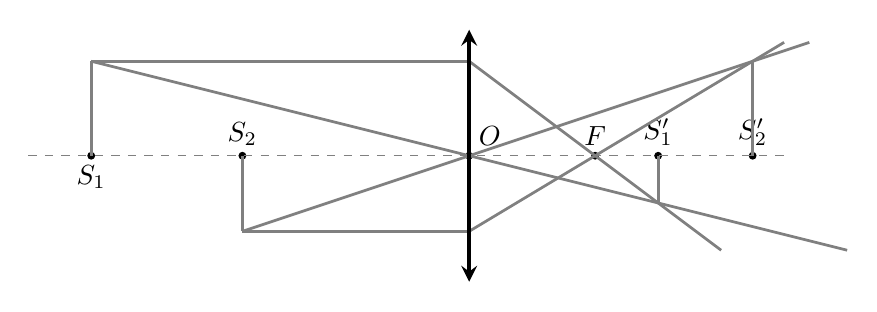
\begin{tikzpicture}[scale=0.8]
    \filldraw[black] (2,0) circle (1.5pt) node[anchor=south] {$F$};
    \filldraw[black] (0,0) circle (1.5pt) node[anchor=south west] {$O$};
    \filldraw[black] (-3.6,0) circle (1.5pt) node[anchor=south] {$S_2$};
    \filldraw[black] (-6,0) circle (1.5pt) node[anchor=north] {$S_1$};

    \filldraw[black] (4.5,0) circle (1.5pt) node[anchor=south] {$S^\prime_2$};
    \filldraw[black] (3,0) circle (1.5pt) node[anchor=south] {$S^\prime_1$};

    \draw[gray] [dashed,-] (-7,0) -- (5,0);
    \draw[gray, line width=1pt] (-6,0) -- (-6,1.5);
    \draw[gray, line width=1pt] (-6,1.5) -- (6,-1.5);
    \draw[gray, line width=1pt] (3,-0.75) -- (3,0);
    \draw[gray, line width=1pt] (-6,1.5) -- (0,1.5);
    \draw[gray, line width=1pt] (0,1.5) -- (4,-1.5);

    \draw[gray, line width=1pt] (-3.6,0) -- (-3.6,-1.2);
    \draw[gray, line width=1pt] (-3.6,-1.2) -- (5.4,1.8);
    \draw[gray, line width=1pt] (4.5,1.5) -- (4.5,0);
    \draw[gray, line width=1pt] (-3.6,-1.2) -- (0,-1.2);
    \draw[gray, line width=1pt] (0,-1.2) -- (5,1.8);

    \draw[line width=1.5pt,>=stealth, <->] (0,-2) -- (0,2);
  \end{tikzpicture}
\end{figure}

Teame, et kui valguskiir langeb peegelpinnale risti, siis liigub see samasugust teed pidi tagasi alguspunkti suunas. Tänu kiirte pööratavuse printsiibile jõuab valguskiir punktidest $S_1'$ ja $S_2'$ tagasi vastavatesse algpunktidesse $S_1$ ja $S_2$. Kumerpeegel on sfääriline, seejuures punkti $S_2'$ poole suunatud kiirte pikendused määravad ära peegli keskpunkti ning punktide $S_1'$ ja $S_2'$ vahekaugus määrab ära joonistatava kaare raadiuse.

\begin{figure}[h]
  \centering
  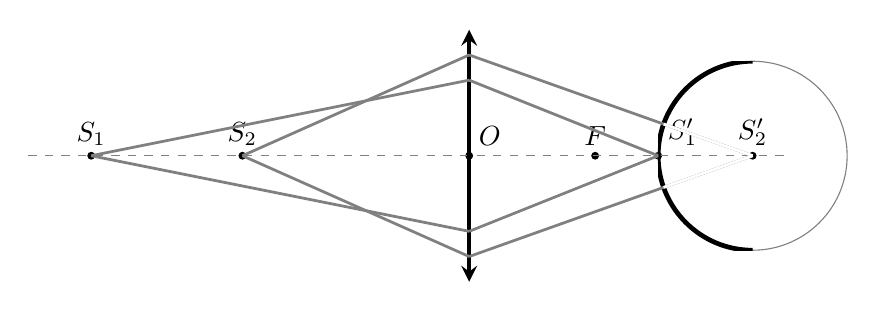
\begin{tikzpicture}[scale=0.8]
    \filldraw[black] (2,0) circle (1.5pt) node[anchor=south] {$F$};
    \filldraw[black] (0,0) circle (1.5pt) node[anchor=south west] {$O$};
    \filldraw[black] (-3.6,0) circle (1.5pt) node[anchor=south] {$S_2$};
    \filldraw[black] (-6,0) circle (1.5pt) node[anchor=south] {$S_1$};

    \filldraw[black] (4.5,0) circle (1.5pt) node[anchor=south] {$S^\prime_2$};
    \filldraw[black] (3,0) circle (1.5pt) node[anchor=south west] {$S^\prime_1$};

    \draw[gray] [dashed,-] (-7,0) -- (5,0);
    \draw[gray] (4.5,0) circle (1.5);
    \draw[line width=1.5pt,>=stealth, <->] (0,-2) -- (0,2);

    \begin{scope}
      \clip (3,-1.5) rectangle (4.5,1.5);
      \draw[black, line width=1.7pt] (4.5,0) circle(1.5);
    \end{scope}

    \draw[gray, line width=1pt] (-6,0) -- (0,-1.2);
    \draw[gray, line width=1pt] (0,-1.2) -- (3,0);
    \draw[gray, line width=1pt] (-6,0) -- (0,1.2);
    \draw[gray, line width=1pt] (0,1.2) -- (3,0);

    \draw[gray, line width=1pt] (-3.6,0) -- (0,-1.6);
    \draw[gray, line width=1pt] (0,-1.6) -- (4.5,0);
    \draw[gray, line width=1pt] (-3.6,0) -- (0,1.6);
    \draw[gray, line width=1pt] (0,1.6) -- (4.5,0);
    \begin{scope}
      \clip (3,-1.5) (4.5,0) circle(1.5);
      \draw[white, line width=1pt] (0,1.6) -- (4.5,0);
      \draw[white, line width=1pt] (0,-1.6) -- (4.5,0);
    \end{scope}

  \end{tikzpicture}
\end{figure}
\probend
\bigskip

% L47
\setAuthor{Kaarel Hänni}
\setRound{piirkonnavoor}
\setYear{2021}
\setNumber{G 3}
\setDifficulty{3}
\setTopic{TODO}

\prob{Joogid}
\solu
Osas (a) antud jooke ei ole võimalik kokku segada. Esiteks on ilmselge, et mitme järjestikuse segamise tulemusel saadud jooki saab valmistada ka kolmest anumast sellesse jooki pandud veekoguste ühekordse segamisega~\pp{0,5}.\par
Näitame nüüd, et nii pole aga võimalik valmistada $\SI{1.5}{\kilo\gram}$ jooki temperatuuril $\SI{13}{\celsius}$. Oletame, et sellise joogi saab valmistada segades koguse $x$ vedelikku temperatuuril $\SI{10}{\celsius}$ ja koguse $y=\num{1.5}-x$ vedelikke temperatuuril vähemalt $\SI{20}{\celsius}$~\pp{1,5}. Sellisel juhul
\begin{align*}
x\cdot 10+y\cdot 20 &\leq 1.5\cdot 13 \\
10x+30-20x &\leq 19.5 \\
10.5 &\leq 10 x \\
x &> 1,
\end{align*}
aga algselt oli temperatuuril $\SI{10}{\celsius}$ vett ainult $\SI{1}{\kilo\gram}$, seega $x\leq 1$ ja viimane võrratus on võimatu \pp2.

Osas (b) antud jooke ei ole võimalik kokku segada, sest energiat oleks lõpus vähem kui alguses. Seda saab näha järgnevalt. Energia jäävuse tõttu peab enne ja pärast segamist vee keskmine temperatuur olema sama \pp{1}. Algselt on keskmine temperatuur $$\frac{\SI{10}{\celsius} \cdot \SI{1}{\kg} +\SI{20}{\celsius} \cdot \SI{1}{\kg}+\SI{30}{\celsius} \cdot \SI{1}{\kg}}{3\text{kg}}=\SI{20}{\celsius}.  \quad \pp{1}$$
Pärast selliste jookide segamist oleks ülejäänud $3-5\cdot 0.5=\SI{0.5}{\kilo\gram}$ vett temperatuuril ülimalt $\SI{30}{\celsius}$, sest see oli kõrgeim algne temperatuur)~\pp{1}. \par
Seetõttu on vee keskmine temperatuur pärast selliste jookide segamist ülimalt
$$\frac{\SI{0.5}{\kg}\cdot(\SI{12}{\celsius} +\SI{17}{\celsius} +\SI{18}{\celsius}+\SI{20}{\celsius} +\SI{22}{\celsius}+\SI{30}{\celsius})}{\SI{3}{\kg}}=\SI{19.8}{\celsius},$$
mis on vähem kui algne keskmine temperatuur \pp1. Seega selliseid jooke ei saa segada.
\probend
\bigskip

% L48
\setAuthor{Oleg Košik}
\setRound{lõppvoor}
\setYear{2021}
\setNumber{G 3}
\setDifficulty{3}
\setTopic{TODO}

\prob{Lääts ja ekraan}
\solu
\par
\begin{figure}[!h]
  \centering
  \begin{minipage}[c]{0.39\textwidth}
    \includegraphics[width=\textwidth]{2021-v3g-03-yl1.pdf}
  \end{minipage}
  \hfill
  \begin{minipage}[c]{0.60\textwidth}
    \vspace*{-2pt}
    \includegraphics[width=\textwidth]{2021-v3g-03-yl2.pdf}
  \end{minipage}
\end{figure}

Olgu $A$ valgusallikas, $B$ tema kujutis läätses ning $CD$ lääts.

Kui ekraan asub läätsest 10 ja 60 cm vahel, tekivad ekraanile kaks kontsentrilist ringi (vasakpoolne joonis): hele väiksem ring diameetriaga $GH$ asub tumeda ringi diameetriga $EF$ sees. Aladele EG ja HF valgusallika valgus ei jõua.

Eemdaldades läätse ekraanist saavad punktid $E$ ja $G$ kokku üheks nagu ka punktid $F$ ja $H$. Ekraani katab ühtlaselt valgus, nagu läätse poleks (parempoolne joonis).

Olgu $x=|AO|$ kaugus valgusallika ja läätse vahel, $r=|OC|$ läätse raadius ning $R=|KE|$. Ülesande tingimustest $|BO|=\SI{10}{cm}$, $|KO|=\SI{60}{cm}$ ning seega $|BK|=\SI{50}{cm}$. Sarnastest kolmnurkadest $AOC$ ja $AKE$ saame
\[
  \frac{r}{R}=\frac{x}{x+60}.
\]
Sarnastest kolmnurkadest $BOD$ ja $BKE$ aga
\[
  \frac{r}{R}=\frac{10}{50}.
\]
Kokkuvõttes saame võrrandi $\displaystyle{\frac{x}{x+60}=\frac{10}{50}}$, mille lahendiks on $x=\SI{15}{cm}$.

Läätse valemist nüüd
\[
  \frac{1}{10}+\frac{1}{15}=\frac{1}{f}\quad \Rightarrow \quad f=\SI{6}{cm}.
\]
\probend
\bigskip

% L49
\setAuthor{Kaarel Hänni}
\setRound{lahtine}
\setYear{2022}
\setNumber{G 3}
\setDifficulty{3}
\setTopic{TODO}

\prob{Kõnd eskalaatoril}
\solu
\emph{Lahendus 1:} Kuna $a \gg b$, siis nurgad on väiksed ning saab kasutada väikeste nurkade lähendusi, $ sin(\alpha) \approx tan( \alpha) \approx \alpha $. Valgus levib kiireimal võimalikul moel. Seega võib eeldada, et Sandra muudab eksalaatorile jõudes enda liikumissuunda nii, nagu valgus murduks.\\
Snelli seadus $ \frac{sin(\beta)}{sin(\alpha)} = \frac{\beta}{\alpha} = \frac{v+u}{v} $ , kus nurgad $\alpha$ ja $\beta$ on mõõdetud külje $a$  suhtes.\\
Geomeetriast: $ tan(\beta) + tan(\alpha) = \beta + \alpha =\frac{2b}{a}$\\
Vastuseks: $ \beta = \frac{2b}{a} \frac{u+v}{u+2v} \approx \SI{0,0286}{\radian}$\\


\emph{Lahendus 2:} Olgu trajektoori horisontaalne kaugus vasakust äärest poole kõrguse juures $x$. Trajektoori aeg on sellisel juhul $\frac{\sqrt{x^2+(a/2)^2}}{v} + \frac{\sqrt{(b-x)^2+(a/2)^2}}{v+u}$, vaja leida $x$ mille korral aeg on minimaalne. Võttes tuletise, saame et $\frac{2x}{2\sqrt{x^2+(a/2)^2}v} + \frac{-2(b-x)}{2\sqrt{(b-x)^2+(a/2)^2}(v+u)} = 0$. Kasutades lähendust, et $a$ on palju suurem, saame $\frac{2x}{av} + \frac{-2(b-x)}{a(v+u)} = 0$, kust $x = \frac{vb}{2v+u}$ ja $\beta = \frac{2b}{a} \frac{u+v}{u+2v}$.
\probend
\bigskip

% L50
\setAuthor{Kaarel Kivisalu}
\setRound{piirkonnavoor}
\setYear{2022}
\setNumber{G 3}
\setDifficulty{3}
\setTopic{TODO}

\prob{Liumägi}
\solu
\emph{Lahendus 1}:
Kalpinna pikkus on $h/\sin \alpha$ \p{0,5}. Horisontaalse pinna pikkus on $l-h/\tan \alpha$ \p{0,5}.
Hõõrdejõud kaldpinnast alla lastes on $F=\mu g \cos \alpha$ \p2. Energia jäävus (potentsiaalse energia muut on võrdne hõõrdejõu tööga):
\begin{equation*}
mgh = \mu mg \cos \alpha \cdot \frac{h}{\sin \alpha} + \mu mg \cdot \left(l- \frac{h}{\tan \alpha}\right). \quad \p4
\end{equation*}
Järelikult $\mu=h/l$ \p1.

\emph{Lahendus 2}:
Kiirendus kaldpinnast alla lastes on $a_1=g \sin \alpha - \mu g \cos \alpha$ \p2. Kalpinna pikkus on $h/\sin \alpha$ \p{0,5}. Järelikult kiirus kaldpinna lõpus on
\begin{equation*}
  v=\sqrt{\frac{2a_1h}{\sin \alpha}}. \quad \p{1,5}
\end{equation*}
Horisontaalse pinna pikkus on $l-h/\tan \alpha$ \p{0,5}. Kuna üleminek kaldpinnalt horisontaalsele pinnale on sujuv, siis kiirus ei muutu. Kiirendus horisontaalsel pinnal on $a_2= - \mu g $. Kuna liumäe lõpus peab alla lastes seisma jääma, siis
\begin{equation*}
  v=\sqrt{-2a_2\left(l-\frac{h}{\tan \alpha}\right)}.\quad \p{1,5}
\end{equation*}
Järelikult
\begin{equation*}
  2\mu g\left(l-\frac{h}{\tan \alpha}\right)=\frac{2h(g\sin \alpha - \mu g \cos \alpha)}{\sin \alpha}, \quad \p1
\end{equation*}
võrrantit lihtsustades saame, et $\mu=h/l$ \p1.
\probend
\bigskip

% L51
\setAuthor{Richard Luhtaru}
\setRound{lõppvoor}
\setYear{2022}
\setNumber{G 3}
\setDifficulty{3}
\setTopic{TODO}

\prob{Silinder}
\solu
\
Jagame silindri kaheks poolsilindriks. Me võime vaadelda kumbagi poolsilindrit kui hästi laia juhet, mille pikkus on $\ell = \pi r$ ja ristlõikepindala on $S = \tau h$. Kummagi poolsilindri takistus on seega
\begin{equation*}
    R = \rho \frac{\ell}{S} = \frac{\rho \pi r}{\tau h}
\end{equation*}

Kuna kaks ``juhet'' on ühendatud rööbiti, siis kogutakistus A ja B vahel on
\begin{equation*}
    R_{AB} = \frac{1}{2}R = \frac{\rho \pi r}{2\tau h}
\end{equation*}
\probend
\bigskip

% L52
\setAuthor{Valter Kiisk}
\setRound{lahtine}
\setYear{2023}
\setNumber{G 3}
\setDifficulty{3}
\setTopic{TODO}

\prob{Kummipael}
\solu
Esimese katse jaoks saame jõudude tasakaalutingimuse $k\Delta L=mg$, kus $k$ on kummipaela jäikustegur ja $m$ on koormise mass (mõlemad tundmatud). Siit saame avaldada suhte $mg/k=\Delta L$. Teises katses on kummipael juba algselt tugevasti deformeeritud olekus, kus tõmbejõud kummipaelas on $kL$ (sest pikkuse muut on $L$). Eeldame, et seetõttu läbivajumine $x\ll L$. Sel juhul, ühelt poolt, läbivajumisest tingitud kummipaela pikenemine on tühine ja seeläbi ka pinge paelas jääb peaaegu muutumatuks. Teiselt poolt, kummipael moodustab horisontaalsihiga nurga $\varphi\approx x/L$. Piki kummipaela suunatud jõu $kL$ projektsioon vertikaalsihile on siis ilmselt $kL\sin\varphi\approx kL\varphi\approx kx$. Kuivõrd kuumipaelal on nüüd kaks poolt, mis mõlemad ühtviisi panustavad koormise $mg$ tasakaalustamisse, siis $2kx=mg$, millest
\[
x =\frac{mg}{2k} =\frac{\Delta L}{2} = \SI{1}{cm}.
\]
\probend
\bigskip

% L53
\setAuthor{Marten Rannut}
\setRound{piirkonnavoor}
\setYear{2023}
\setNumber{G 3}
\setDifficulty{3}
\setTopic{TODO}

\prob{Ökonoomne sõit}
\solu
Ülesandes pole vahet, kas leiame kütusekulude suhte $\SI{100}{\m}$ või $\SI{100}{\km}$ kohta \p{1} (juhul kui õpilane arvutab kütusekulud $\SI{100}{\km}$ jaoks, siis anda see punkt, kui õpilane leiab korrektselt $E_l$ $\SI{100}{\km}$ jaoks). Linnas kiirendab auto iga $\SI{100}{\m}$ tagant kiiruseni $v_l = \SI{40}{\km\per\hour} \approx \SI{11.1}{\m\per\s}$ \p{1}. Selleks kulub energia
\begin{equation*}
    E_l = \frac{mv_l^2}{2} = \frac{\SI{1500}{\kg}\cdot (\SI{11.1}{\m\per\s})^2}{2} \approx \SI{92.4}{\kJ}. \quad \p{1}
\end{equation*}

Maanteesõidul on auto kiirus $v_m = \SI{90}{\km\per\hour} = \SI{25}{\m\per\s}$ \p{1}. Auto poolt tehtav töö õhutakistuse ületamiseks on $E_m = Fs$ \p{1}, seega
\begin{equation*}
    E_m = cv^2s = \SI{1.3}{\kg\per\m}\cdot \left(\SI{25}{\m\per\s}\right)^2 \cdot \SI{100}{\m} \approx \SI{81.3}{kJ}.\quad \p{1}
\end{equation*}

Kuna mootori kasutegur on mõlemal juhul sama, siis kütusekulude suhe on võrdne kuluva energia suhtega \p{1}. Seega kütusekulude suhe on
\begin{equation*}
    \frac{k_m}{k_l} = \frac{\SI{81.3}{\kJ}}{\SI{92.4}{\kJ}} \approx \num{0.88}. \quad\p{1}
\end{equation*}
(või $k_l/k_m \approx \num{1.14}$).
\probend
\bigskip

% L54
\setAuthor{Aigar Vaigu}
\setRound{lõppvoor}
\setYear{2023}
\setNumber{G 3}
\setDifficulty{3}
\setTopic{TODO}

\prob{Lääts ja kaks peeglit}
\solu
\par
Tõmbame punktist $A$ väljuva horisontaalse sinise kiire, pärast poolläbilaskvas peeglis peegeldumist on see vertikaalne, läätses koondab selle optilisele peateljele, kus see peegeldub ning jõuab läätseni tagasi. Teiseks kiireks tõmbame lilla kiire punktist $A$ poolläbilaskva peegli keskpunkti, pärast läätse läbimist liigub see edasi otse (kuna läätse fookus on poolläbilaskva peegli keskpunktis) ning lõikub läätse tasandis algse kiirega. Selle punkti näol on tegu $A$ kujutisega. Analoogselt konstrueerime punkti $B$ kujutise läätse tasandis. Objekti $AB$ kujutis läätse tasandis on sama suur kui oli algne kujutis. Tasub märkida, et seda kujutist näeb ülevalt vaadates (kui oleks tegu tavalise peegliga näeks seda ainult poolläbilaskva peegli ja läätse vahel asudes).

Nii algsel objektil kui selle kujutisel läätse tasandis on ka kujutised poolläbilaskvas peeglis nagu oleks neil tavalistes peeglites. Konstrueerime ka need.

Kokku tekib kolm kujutist. Ülemist kujutist näeb altpoolt poolläbilaskvat peeglit vaadates. Parempoolset kujutist näeb vasakult poolt poolläbilaskvat peeglit vaadates. Nagu juba mainitud, siis kujutist läätse tasandis näeme vaadates ülevaltpoolt.

Kuna siin skeemis on poolläbilaskev peegel, siis kujutised on mõnevõrra tumedamad võrreldes tavalise peegliga. Alumine kujutis 2 korda tumedam vaadates seda poolläbilaskva peegli ja läätse vahelt ning 4 korda tumedam vaadates seda läbi poolläbilaskva peegli. Parempoolne ja ülemine kujutis on mõlemad 4 korda tumedamad.
\begin{center}
  \includegraphics[width=0.86\textwidth]{2023-v3g-03-yl.png}
\end{center}
\probend
\bigskip

% L55
\setAuthor{Richard Luhtaru}
\setRound{lahtine}
\setYear{2024}
\setNumber{G 3}
\setDifficulty{3}
\setTopic{TODO}

\prob{Valguskaabel}
\solu
Defineerime nurgad $\alpha$ ja $\beta$ nagu joonisel. Valgus levib ilma kadudeta siis, kui $\beta$ on piisavalt suur ja kaabli südamikus toimub täielik sisepeegeldumine. Seega piirjuhul
\begin{equation*}
    n_1 \sin \beta = n_2.
\end{equation*}

\begin{figure}[h]
    \centering
    \includegraphics[width=.7\linewidth]{2024-lahg-03-yl.pdf}
\end{figure}

Murdumisseadusest saame samuti
\begin{equation*}
    n_0 \sin \theta_0 = n_1 \sin \alpha \implies n_0 \text{NA} = n_1 \sin \alpha \implies \text{NA} = \frac{n_1 \sin \alpha}{n_0}.
\end{equation*}

Kuna $\alpha$ ja $\beta$ on täisnurkse kolmnurga nurgad, siis $\beta = \ang{90} - \alpha$, seega $\sin \beta = \cos \alpha$. Seega
\begin{equation*}
    n_1 \cos\alpha = n_2 \implies \cos \alpha = \frac{n_2}{n_1} \implies \sin\alpha = \sqrt{1-\cos^2\alpha} = \sqrt{1-\left(\frac{n_2}{n_1}\right)^2}
\end{equation*}
ning
\begin{equation*}
    \text{NA} = \frac{n_1}{n_0}\sin\alpha = \frac{n_1}{n_0}\sqrt{1-\left(\frac{n_2}{n_1}\right)^2} = \frac{\sqrt{n_1^2-n_2^2}}{n_0}.
\end{equation*}
\probend
\bigskip

% L56
\setAuthor{Hans Daniel Kaimre}
\setRound{piirkonnavoor}
\setYear{2024}
\setNumber{G 3}
\setDifficulty{3}
\setTopic{TODO}

\prob{Valgusdioodid}
\solu
Kuivõrd LEDide nominaalne voolutugevus on võrdne, on mõistlik need ühendada omavahel jadamisi, nii nagu Mari seda tegi. Pingelang üle LEDide normaaltingimustel on $U_1+U_2=\SI{3}{\V}+\SI{3.5}{\V}=\SI{6.5}{\V}$, mis on tunduvalt vähem kui patarei klemmipinge $U=\SI{12}{V}$. Järelikult tuleb vooluringi ühendada LEDidega jadamisi takisti, millel pingelang oleks $U_R=U-U_1-U_2=\SI{12}{\V}-\SI{6.5}{\V}=\SI{5.5}{\V}$. Takisti väärtuse saame leida lihtsalt Ohmi seadusest, kuna takistit läbiv voolutugevus peab olema võrdne LEDe läbiva voolutugevusega: $R=U_R/I_1=\SI{5.5}{\V}/\SI{30}{\milli\A}=\SI{183}{\ohm}$.

\begin{figure}[h]
    \centering
    \includegraphics[width=0.5\linewidth]{2024-v2g-03-yl.pdf}
\end{figure}
\probend
\bigskip

% L57
\setAuthor{Sandra Schumann}
\setRound{lõppvoor}
\setYear{2024}
\setNumber{G 3}
\setDifficulty{3}
\setTopic{TODO}

\prob{Leedid}
\solu
Patareid lühistada ei tohi, seega dioode otse patarei külge ühendada ei tohi. Järelikult peavad dioodid olema mingis kombinatsioonis jadamisi takistitega. Tahame, et dioodide põlemise korral läbiks neid voolutugevus $\SI{20}{\mA}$. Ilmselt peab vähemalt selline voolutugevus läbima ka vähemalt ühte takistit. Kui see voolutugevus läbib \SI{300}{\ohm} takistit, siis sellel on pingelang $\SI{6}{\V}$, läbides \SI{360}{\ohm} takistit oleks pinge \SI{7.2}{\V}.

Märkame nüüd, et dioodide põlemiseks vajalike päripingete ja soovitud voolutugevustel olevate patareide pingelangude summad saavad võrduda patarei pingega kahel juhul: punane dioodi jadamisi \SI{360}{\ohm} takisti ja patareiga ning sinine diood jadamisi \SI{300}{\ohm} takisti ja patareiga.

Rakendades tingimust, et vastavat värvi lülitit vajutades peab minema põlema vastavat värvi diood, saame kaks võimalikku skeemi:
\begin{center}
  \begin{tikzpicture}[scale=0.7]
    \draw (0,0) to[battery1, l_=\SI{9}{\V}, invert] (0,6) to[short] (2,6) to[short] (6,6) to[R=\SI{300}{\ohm}] (6,3.5) to[short, *-*] (6,2) to[nos, color=red, l=punane, red] (6,0) to[short, -*] (2,0) -- (0,0);
    \draw (2,6) to[R, l_=\SI{360}{\ohm}, *-] (2,3.5) to[short, *-*] (2,2) to[nos, color=blue, l_=sinine, blue] (2,0);

    \draw (2,3.5) to[led, l=punane, fill=red, red] (6,3.5);
    \draw (2,2) to[led, l_=sinine, invert, fill=blue, blue] (6,2);
  \end{tikzpicture}
  \hspace{-1cm}
  \begin{tikzpicture}[scale=0.7]
    \draw (1,0) to[battery1, l=\SI{9}{\V}, invert] (1,6) to[short] (2,6) to[short] (6,6) to[R=\SI{300}{\ohm}] (6,3.5) to[led, l=sinine, fill=blue, blue] (6,2) to[nos, color=blue, l=sinine, blue] (6,0) to[short, -*] (2.75,0) -- (1,0);
    \draw (2.75,6) to[R, l=\SI{360}{\ohm}, *-] (2.75,3.5) to[led, l=punane, fill=red, red] (2.75,2) to[nos, color=red, l=punane, red] (2.75,0);
  \end{tikzpicture}
\end{center}

Meil peab veel kehtima ka tingimus, et mõlema lüliti vajutamisel ei põleks kumbki diood. See on tõene ainult vasakpoolse skeemiga. Seega just see skeem tulebki koostada.
\probend
\bigskip

% L58
\setAuthor{Erkki Tempel}
\setRound{lahtine}
\setYear{2018}
\setNumber{G 4}
\setDifficulty{4}
\setTopic{TODO}

\prob{Kahurid}
\solu
\
Kahurist $A$ tulistatud kuul jõuab haripunkti siis, kui selle vertikaalne kiiruse komponent on $0$, ehk ajahetkel $t_0 = \frac{v_A\sin\alpha}{g} = \SI{7}{s}$. Kahurikuulid põrkuvad seega kokku momendil $t_0 + t_1 = \SI{12}s$. Sellel hetkel on kahurist $A$ lastud kuuli ja kahuri $B$ horisontaalne vahekaugus $v_A\cos\alpha(t_0 + t_1) - l = v_{Bx}t_1$, kus $v_B$ on kahurist $B$ tulistatud kuuli algkiirus. Niisiis, $v_{Bx} = \frac{v_A\cos\alpha(t_0 + t_1) - l}{t_1} = \SI{-91.0}{m/s}$.

Selleks, et kuulid vertikaaltasandis ajehetkel $t_0 + t_1$ kokku saaksid, peab kehtima
\[
v_A\sin\alpha (t_0 + t_1) - \frac{g(t_0 + t_1)^2}{2} = v_yt - \frac{gt_1^2}{2},
\]
ehk
\[
v_{B_y} = v_A\sin\alpha \left(\frac{t_0}{t_1} + 1\right) - \frac{g(t_0 + t_1)^2}{2t_1} + \frac{gt_1}{2} = \SI{49}{m/s}.
\]
Niisiis,
\[
v_B = \sqrt{v_{Bx}^2 + v_{By}^2} = \SI{103}{m/s}.
\]
\probend
\bigskip

% L59
\setAuthor{Kaarel Hänni}
\setRound{lahtine}
\setYear{2019}
\setNumber{G 4}
\setDifficulty{4}
\setTopic{TODO}

\prob{Laetud tasand}
\solu
Ühe laengu poolt tasandile avaldatav jõud on võrdne ja vastasmärgiline tasandi poolt laengule avaldatava jõuga. Seega on tasandile kokku mõjuv jõud 0 siis ja ainult siis, kui tasandi poolt laengutele avaldatud jõudude summa on 0. Tasandi elektriväli on konstantne ja risti tasandiga (ja tasandi eri pooltel erisuunaline). Seega on tasandi poolt laengutele avaldatud jõudude summa 0 siis ja ainult siis, kui kummalgi pool tasandit on võrdne arv laenguid. Laenguid on kokku paaritu arv, seega see on võimatu.
\probend
\bigskip

% L60
\setAuthor{}
\setRound{piirkonnavoor}
\setYear{2019}
\setNumber{G 4}
\setDifficulty{4}
\setTopic{TODO}

\prob{Vaakum}
\solu
\osa Toru tühjakspumpamine tähendab sisuliselt õhu väljasurumist torust, tehes tööd välisrõhu $p$ vastu. \pp{1} Õhk mõjub kuulikesele resultatiivse jõuga $pS$, kus toru ristlõikepindala $S=\pi(d/2)^2=\SI{0.79}{cm^2}$. \pp{1} Jõudu $pS$ tuleb rakendada teepikkusel $\ell$, nii et tehtud töö $A=pS\ell$. \pp{1}   $A=\SI{101300}{Pa}\cdot \SI{7.9e-5}{m^2}\cdot\SI{1}{m}\approx\SI{8.0}{J}$. \\
\osa Kuulikese mass: \[m=\rho V=\rho(4/3)\pi(d/2)^3=\pi \rho d^3/6= \pi\cdot \SI{7.9}{g/cm^3}\cdot (\SI{1}{cm})^3/6 =\SI{4.1}{g}\] \pp{1} Kuna kuulike liigub eeldatavasti hulga aeglasemalt kui on heli kiirus, siis talle mõjub praktiliselt konstantne kiirendav jõud $pS$, jällegi teepikkusel $\ell$. Järelikult eelmises punktis leitud töö $A$ annab ühtlasi kuulikese kineetilise energia toru teises otsas. \pp{1} Kuna $mv^2/2=A$, siis $v=\sqrt{2A/m}$. \pp{1}
\[
v=\sqrt{\frac{2\times \SI{8.0}{J}}{\SI{0.0041}{kg}}}\approx\SI{62}{m/s}\,\text{\pp{1}}
\]
Alternatiivselt võib kasutada ka tuntud valemit ühtlase kiirenduse jaoks, $v^2-v_0^2=2a\ell$, kus algkiirus $v_0=0$ ja kiirendus $a=pS/m$.
\probend
\bigskip

% L61
\setAuthor{}
\setRound{lõppvoor}
\setYear{2019}
\setNumber{G 4}
\setDifficulty{4}
\setTopic{TODO}

\prob{Konveier}
\solu
Olles täielikult esimesel lindil, on plaadi kiirus $v_1$ ning teisel lindil $v_2$. Plaadi kiirus muutub üleminekukohas $v_1$-lt $v_2$-le, kui hõõrdejõud teise konveierilindiga ületab hõõrdejõu esimese konveierilindiga. Olgu plaadi mass $M$ ning plaadi joontihedus piki konveierit $\rho = M/l$. Piirjuhul saame hõõrdejõudude võrdsusest:
$$\mu_{1}M_1g = \mu_{2}M_2g$$
kus $M_1$ ja $M_2$ on vastavalt esimese ja teise lindi peal oleva plaadi osa massid. Olgu esimesel lindil oleva osa pikkus $l_1$ ning teisel osal $l_2$. Kasutades joontihedust saame:
$$\mu_{1} \rho l_1 g = \mu_{2}\rho l_2 g$$.
Taandades ühised kordajad saame võrrandisüsteemi:
$$\mu_{1} l_1 = \mu_{2} l_2$$
$$l_1 + l_2 = l$$
Siit saame avaldada $l_1$-e:
$$l_1 = \frac{l}{1+\frac{\mu_{1}}{\mu_{2}}}$$

\begin{center}
\includegraphics[scale=0.5]{2019-v3g-04-yl.png}
\end{center}


Joonisel on kujutatud plaadi algasend, lõppasend ning piirjuht, kus kiirus muutub (tühiselt väikese aja jooksul). Algasendist piirjuhuni läbib plaat vahemaa $x - l_1$ kiirusel $v_1$. Piirjuhust lõppasendini läbib plaat vahemaa $x - l_2$ kiirusel $v_2$. Seega koguaeg:
$$t = \frac{x - l_1}{v_1} + \frac{x - l_2}{v_2}$$
Asendades saame:
$$t=\frac{v_2 x - v_2 l_1 + v_1 x - v_1 l_2}{v_1 v_2} =$$
$$\frac{x(v_1 + v_2) - lv_1 - l_1 v_2 + l_1 v_1}{v_1 v_2} =$$
$$\frac{x(v_1 + v_2) - lv_1 + \frac{l(v_1 - v_2)}{1+\frac{\mu_{1}}{\mu_{2}}}}{v_1 v_2}$$
\probend
\bigskip

% L62
\setAuthor{Richard Luhtaru}
\setRound{lahtine}
\setYear{2020}
\setNumber{G 4}
\setDifficulty{4}
\setTopic{TODO}

\prob{Noova}
\solu
Vaatleme jäänuki liikumist aja $t$ jooksul, selle aja jooksul liigub jäänuk vahemaa $vt$. Näeme, et ristisihis liigub jäänuk vahemaa $vt \sin \theta$, seega kasutades väikeste nurkade lähendusi, on Jarli poolt mõõdetav nurk nende kahe positsiooni vahel $\alpha = vt\sin\theta/D$ ja näiv vahemaa, mille jäänuk nende hetkede vahel läbib on
\begin{equation*}
	x' = \alpha D = vt\sin\theta.
\end{equation*}

\begin{figure}[h]
\centering
\includegraphics[width=0.25\linewidth]{2020-lahg-04-yl.pdf}
\end{figure}

Küll aga tuleb arvestada ka sellega, et jäänuk liigub selle aja jooksul $vt \cos\theta$ vaatesihis Jarlile lähemale, mistõttu teepikkus, mille valgus peab Jarlini jõudmiseks läbima, lüheneb ja seega näiv aeg kahe hetke vahel $t'$ ei ole võrdne tegeliku ajaga $t$. Kuna esimesel hetkel on jäänuki kaugus Jarlist $D$ ning teisel juhul $D-vt\cos\theta$ (kasutades lähendust, et $D$ on väga suur), siis näiv aeg kahe hetke vahel on
\begin{equation*}
t' = t_2 - t_1 = \left(t + \frac{D-vt\cos\theta}{c}\right) - \frac{D}{c} = t\left(1 - \frac{v\cos\theta}{c}\right).
\end{equation*}

Seetõttu Jarli poolt mõõdetav näiv kiirus on
\begin{equation*}
v' = \frac{x'}{t'} = \frac{v \sin \theta}{1- \frac{v}{c}\cos\theta}.
\end{equation*}

Näeme, et näiv kiirus võib olla tõesti suurem kui $c$. Näiteks kui $\theta = 45^\circ$ ja $v = \frac{7}{5\sqrt 2}c$ (mis on väiksem kui $c$), siis
\begin{equation*}
v' = \frac{\frac{7}{5\sqrt 2} c \cdot \frac{1}{\sqrt 2}}{1- \frac{7}{5\sqrt 2} \cdot \frac{1}{\sqrt 2}} = \frac{7}{3} c > c.
\end{equation*}

\textit{Märkus.} Selline nähtust, kus näiv kiirus on valguse kiirusest suurem (ingl. k. \textit{superluminal motion}), on märgatud mitmete astronoomiliste objektide korral. Üks suuremaid näivaid kiirusi on mõõdetud kvasarijoa korral, mille näivaks kiiruseks mõõdeti $\num{9.6}c$.
\probend
\bigskip

% L63
\setAuthor{}
\setRound{piirkonnavoor}
\setYear{2020}
\setNumber{G 4}
\setDifficulty{4}
\setTopic{TODO}

\prob{Elektriruut}
\solu
\begin{wrapfigure}{r}{0.3\textwidth}
    \vspace{-30pt}
	\includegraphics[width=0.28\textwidth]{2020-v2g-04-yl.jpg}
	\vspace{-40pt}
\end{wrapfigure}
Tähistame joonisel punktid A, B, C
ja D. Paneme tähele, et kuna
A ja C on ühendatud omavahel
juhtmega, mille takistuse võime
lugeda nulliks, siis A = C \pp{1}. Samal
põhjusel B = D \pp{1}. Nüüd võime
skeemi ümber joonistada nii, nagu
näidatud joonisel 2. \pp{2}

Sümmeetria tõttu ei läbi punktide A, C ja B, D vahelist silda kunagi vool \pp{2}, seega lihtsustub skeem
kujule, kus on vaid neli ülejäänud takistit \pp{1}, mille kogutakistuseks tuleb $\frac{2R}{2} = R$ \pp{1}
\probend
\bigskip

% L64
\setAuthor{}
\setRound{lõppvoor}
\setYear{2020}
\setNumber{G 4}
\setDifficulty{4}
\setTopic{TODO}

\prob{Tasakaaluliikur}
\solu
Hannese liikumist saab vertikaalsuunas käsitleda vedrupendli võnkumisena. Vedrupendli perioodi valem on: $$T=2\pi \sqrt{\frac{m}{k}}$$ Kuna meie süsteemil on kaks vedru rööbiti, tuleb võngete perioodi valemit veidi muuta. Kahe kõrvuti oleva vedru jäikus on võrdne ühe vedruga, mille jäikus on eelnevate vedurude jäikuste summaga. Seega on meie süsteemi vertikaalsuunaliste võngete periood:
$$T = 2\pi \sqrt{\frac{m}{2k}}$$
Resonants tekib, kui koosinuslaine läbimise sagedus ühtib verikaalse vedrusüsteemi naturaalsagedusega. Seega peab Hannes $\Delta x = \SI{6}{m}$ võrra edasi liikuma sama ajaga, mil teeb masspendel ühe naturaalsagedusel võnke. Seega, resonantsi tekke kiirus:
$$v_\mathrm{resonants}=\frac{\Delta x}{T}=\frac{\Delta x}{2 \pi} \sqrt{\frac{2k}{m}} = \SI{4.678}{m s^{-1}} \approx \SI{4.7}{m s^{-1}}$$
\probend
\bigskip

% L65
\setAuthor{Jaan Kalda}
\setRound{lahtine}
\setYear{2021}
\setNumber{G 4}
\setDifficulty{4}
\setTopic{TODO}

\prob{Kuiv õhk}
\solu
Kui õhk siseneb ruumi, siis vee moolide suhe kogu gaasi moolide arvu ei muutu, olgu need teatud koguse tuppa siseneva õhu jaoks vastavalt $\nu_v$ ja $\nu_k$. Ideaalse gaasi olekuvõrrandist saame vee osarõhu ja kogu rõhu jaoks vastavalt $p_vV=\nu_vRT$ ja $p_kV=\nu_kRT$, millest $p_v = p_k\frac{\nu_v}{\nu_k}$. Arvestades, et kogurõhk on nii toas kui väljas võrdne atmosfäärirõhuga $p_0$, saame suhtelise niiskuse jaoks avaldise $r=\frac{p_v}{p(T)}=\frac{p_0}{p(T)}\frac{\nu_v}{\nu_k}$, kus $p(T)$ tähistab küllastunud auru rõhku sõltuvuses temperatuurist ja on leitav graafikult. Tähistagu $r_v=\frac{p_0}{p(T_v)}\frac{\nu_v}{\nu_k}$ ja $r_s=\frac{p_0}{p(T_s)}\frac{\nu_v}{\nu_k}$ vastavalt suhtelisi niiskusi väljas ja sees. Seega $p(T_v)=p(T_s)\frac{r_s}{r_v}=\frac{p(T_s)}{4}$; graafikult loeme, et $p(T_s)\approx \SI{2,2}{kPa}$ (NB! tüvenumbrite lugemisel tuleb meeles pidada, et tegemist on logaritmilise graafikuga!) ning seega $p(T_v)\approx\SI{550}{Pa}$. Graafikult leiame ka sellele rõhule vastava temperatuuri, $T_v \approx \SI{-1}\celsius$.
\probend
\bigskip

% L66
\setAuthor{Kaido Reivelt}
\setRound{piirkonnavoor}
\setYear{2021}
\setNumber{G 4}
\setDifficulty{4}
\setTopic{TODO}

\prob{Batüskaaf}
\solu
Kuna kasutada on lihtmehhanismid, pole maksimaalne rakendatav jõud oluline, sest Monikal on neid kasutades võimalik avaldada ükskõik kui suuri jõude. Rõhu vahe batüskaafi väljas ja sees on
$$\Delta p=\rho gh. \quad \pp{2}$$

Rõhuvahe avaldab silindrile jõudu
$$F_p=\Delta p S = \rho gh S. \quad \pp{2}$$
Sellise jõuga tuleb tööd teha, et vett batüskaafist välja pumbata. Vee välja pumpamiseks vajalik töö avaldub kui
$$A=F_p\cdot \Delta x= \rho gh S \Delta x. \quad \pp{2}$$

Paneme tähele, et batüskaafist on tarvis välja pumbata kokku $V=\SI{1}{\liter}$ vett, järelikult peab kehtima $V=S\Delta x$ \pp{1}.

Ruumala $V$ batüskaafist välja pumpamiseks on vaja teha tööd $A=\rho g h V$. Kuna teame, et tööd saab teha keskmise võimsusega $P=\SI{100}{\W}$, saame et vee välja pumpamiseks kulub
$$t=\frac{A}{P}=\frac{\rho g h V}{P}=\SI{1009}{\s}. \quad \pp{1}$$
\probend
\bigskip

% L67
\setAuthor{Richar Luhtaru}
\setRound{lõppvoor}
\setYear{2021}
\setNumber{G 4}
\setDifficulty{4}
\setTopic{TODO}

\prob{Sõit jääl}
\solu
Kui auto mass on $m$, siis auto raskusjõud on $F_g = mg$ ja maksimaalne ratastele mõjuv hõõrdejõud on $F_h = \mu mg$. Maksimaalne autole mõjuda saav kiirendav/pidurdav jõud on maksimaalne hõõrdejõud (muidu hakkaksid rattad libisema), seega auto maksimaalne kiirendus on $a_{max} = \frac{F_h}{m} = \mu g$ ja minimaalne kiirendus on $a_{min}=-\frac{F_h}{m}= -\mu g$.

On ilmne, et minimaalse sõiduaja korral kiirendab auto kõigepealt maksimaalse kiirendusega $a_{max}$ ja seejärel pidurdab kiirendusega $a_{min}$, nii et auto jääks täpselt tee lõpus seisma. Tõepoolest, kui auto kiirendus ei oleks mingil hetkel maksimaalne/minimaalne võimalik, saaks auto sellel ajaperioodil lühikese aja maksimaalselt kiirendada ja pidurdada, vähendades sõiduaega. Kuna $\mu_2 > \mu_1$, siis on maksimaalne kiirendus suurem teisel lõigul ja seega ka kiirendamine muutub pidurdamiseks tee teisel lõigul.

Kulugu autol aeg $t_1$, et jõuda tee keskele, seejärel aeg $t_2$ jõudmaks kohta, kus kiirendamine muutub pidurdamiseks, ja seejärel aeg $t_3$, et jõuda tee lõppu. Vastavad auto kiirendused on $a_1=\mu_1 g$, $a_2=\mu_2 g$ ja $a_3=-\mu_2 g$.

Aja $t_1$ jooksul läbib auto teepikkuse $L$, seega
\[
  L=\frac{\mu_1 g t_1^2}{2} \implies t_1 = \sqrt{\frac{2L}{\mu_1 g}} = \SI{10}{s}.
\]
Tee keskele jõudes on auto kiirus
\[
  v_1 = \mu_1 g t_1 = \mu_1 g \cdot \sqrt{\frac{2L}{\mu_1 g}} = \sqrt{2L\mu_1 g} = \SI{10}{m/s}.
\]
Seejärel peale aja $t_2$ läbimist on auto kiirus
\[
  v_2 = v_1 + \mu_2 g t_2.
\]
Et teise lõigu pikkus on samuti $L$, siis
\[
  L = \frac{v_2^2 - v_1^2}{2a_2} + \frac{0-v_2^2}{2a_3} = \frac{2v_2^2 - v_1^2}{2\mu_2 g},
\]
\[
  v_2 = \sqrt{\frac{2\mu_2 gL+v_1^2}{2}} \approx \SI{12.25}{m/s}.
\]
Seega
\[
  t_2 = \frac{v_2-v_1}{\mu_2 g} \approx \SI{1.12}{s}.
\]
Kuna auto peab tee lõpus seisma jääma, siis
\[
  \Delta v = 0 \implies \mu_1 g t_1 + \mu_2 g t_2 - \mu_2 g t_3 = 0 \implies t_3 = t_2 + \frac{\mu_1}{\mu_2}t_1 \approx \SI{6.12}{s}
\]
ja tee läbimise koguaeg on
\[
  t=t_1+t_2+t_3 \approx \SI{17,24}{s}.
\]
\probend
\bigskip

% L68
\setAuthor{Uku Andreas Reigo}
\setRound{lahtine}
\setYear{2022}
\setNumber{G 4}
\setDifficulty{4}
\setTopic{TODO}

\prob{Kuiv jää}
\solu
Kõik kuiva jää sublimeerimiseks ja soojendamiseks vajalik energia tuleb õhust. Leiame sublimeerimiseks vajaliku energia:
\begin{align*}
    Q_{sub} &= n_{CO_2} \cdot \lambda_{CO_2}\\
    &= \frac{m_{CO_2}}{M_{CO_2}} \cdot \lambda_{CO_2}\\
    &= \frac{m_{CO_2}\cdot \lambda_{CO_2}}{M_{C} + 2\cdot M_{O}}
\end{align*}
Energiatasakaalust teame, et CO\(_2\) sublimeerimiseks ja soojendamiseks (\(Q_1\)) vajaminev energia tuli täielikult õhu jahtumisest (\(Q_2\)) lõpptemperatuurini \(T_{\textup{lõpp}}\), kusjuures \(Q = mc\Delta T\).

\begin{align*}
    Q_{sub} + Q_1 &= Q_2 \\
    Q_{sub} + m_{CO_2}C_{CO_{2}}\cdot(T_{\textup{lõpp}}-T_{0}) &= V_{\textup{tünn}}\rho_{\textup{õhk}}C_{\textup{õhk}}\cdot(T_{\textup{õhk}}-T_{\textup{lõpp}})\\
\end{align*}
Avaldame lõpptemperatuuri:
\begin{equation*}
    T_{\textup{lõpp}} = \frac{V_{\textup{tünn}}\rho_{\textup{õhk}}C_{\textup{õhk}}T_{\textup{õhk}}+m_{CO_2}C_{CO_{2}}T_{0}-Q_{sub}}{m_{CO_2}C_{CO_{2}}+V_{\textup{tünn}}\rho_{\textup{õhk}}C_{\textup{õhk}}}
\end{equation*}
Asendades teatud väärtused sisse, saame \(T_{\textup{lõpp}} = \SI{17,7}{\degreeCelsius}\) 

Rõhu arvutamiseks kasutame ideaalgaasi seadust. Algselt on tünnis \(n_0 =\frac{p_0V_{\textup{tünn}}}{R\cdot T_{\textup{õhk}}}\) mooli erinevaid õhumolekule. Lisandub \(n_{CO_2} = \frac{m_{CO_2}}{M_{C} + 2\cdot M_{O}}\) mooli süsihappegaasi ning lõpptemperatuur on äsja leitud, seega

\begin{align*}
    p_{\textup{lõpp}} &= \frac{nRT}{V}\\
    &=\frac{(\frac{m_{CO_2}}{M_{C} + 2\cdot M_{O}}+\frac{p_0V_{\textup{tünn}}}{R\cdot T_{\textup{õhk}}})R(273,15 + \SI{17,7}{\degreeCelsius})}{V_{\textup{tünn}}}
\end{align*}
asendades sisse teatud väärtused saame \(p_{\textup{lõpp}} = \SI{99.3}{\kilo\pascal}\)

Kui kuiv jää oleks kohe veevannis, siis oleks soojendamiseks tulnud energia just sealt veest (vann on suur, seega vesi ei jäätu ning terve kuiv jää ning kaasnev gaas saab välja). Seega oleks lõplik temperatuur tünnis soojem ning järelikult ka rõhk suurem.
\probend
\bigskip

% L69
\setAuthor{Jarl Patrick Paide}
\setRound{piirkonnavoor}
\setYear{2022}
\setNumber{G 4}
\setDifficulty{4}
\setTopic{TODO}

\prob{Kaks tuba}
\solu
Olgu mõlemas toas algne kütteallikas võimsusega $N$ \p{0,5}. Olgu toas, kus on lisaks kütteallikas võimsusega $P$ temperatuur $T_0$, teises toas temperatuur $T_1$ ja väljas temperatuur $T_2$. Süsteem on tasakaalus kui $T_0 > T_1 > T_2$ \p{0,5}. Paneme kirja võrrandi mõlema toa jaoks kus paremal pool on toast lahkuv soojus ja vasakul pool tuppa sisenev soojus.
\begin{align*}
  N+P&=3k(T_0 - T_2)+k(T_0-T_1), \quad \p2\\
  N+k(T_0-T_1)&=3k(T_1 - T_2). \quad \p2
\end{align*}
Siit saame avaldada temperatuurivahe $T_0-T_1=\frac{P}{5k}$ \p3.
\probend
\bigskip

% L70
\setAuthor{Erkki Tempel}
\setRound{lõppvoor}
\setYear{2022}
\setNumber{G 4}
\setDifficulty{4}
\setTopic{TODO}

\prob{Läätsede kolmnurk}
\solu
\

\begin{figure}[h]
    \centering
    \includegraphics[scale=0.5]{2022-v3g-04-yl.pdf}
\end{figure}
\probend
\bigskip

% L71
\setAuthor{Päivo Simson}
\setRound{lahtine}
\setYear{2023}
\setNumber{G 4}
\setDifficulty{4}
\setTopic{TODO}

\prob{Kondensaatorid}
\solu
Enne laadimise algust on esimese kondensaatori energia
\[E_1=\frac{C_1U_0^2}{2}=4500\,\textrm{J}\]
ja teise energia on null. Laadimise käigus toimub kondensaatorite vahel laengu ümberjaotumine, kuid kogulaeng $q$ säilib. Laadimisprotsess toimub seni, kuni kondensaatorite pinged võrdsustuvad. Lõpp-pinge $U$ saame leida laengu jäävuse seadusest:
\[q=C_1U_0=C_1U+C_2U\quad\implies\quad U=\frac{C_1U_0}{C_1+C_2}=6\,\textrm{kV}.\]
Laadimise lõpuks on kahe kondensaatori koguenergia
\[E_2=\frac{C_1U^2}{2}+\frac{C_2U^2}{2}=\frac{(C_1+C_2)U^2}{2}=1800\,\textrm{J}.\]
Näeme, et see on väiksem kui esimese kondensaatori energia enne laadimise algust. Puuduolev energia eraldus järelikult süsteemist soojusena, peamiselt hõõglambi põlemisel. Otsitav soojushulk on seega
\[Q=E_1-E_2=2700\,\textrm{J}.\]
\emph{Märkus:} ülesande võib lahendada ka vahetulemusi kasutamata. Energia ja laengu jäävustest saame
\[
\begin{cases}
\displaystyle\frac{C_1U_0^2}{2}=\frac{C_1U^2}{2}+\frac{C_2U^2}{2}+Q\\
\,\,C_1U_0=C_1U+C_2U
\end{cases}
\implies Q=\frac{C_1C_2U_0^2}{2(C_1+C_2)}=2700\,\textrm{J}.
\]
\probend
\bigskip

% L72
\setAuthor{Marten Rannut}
\setRound{piirkonnavoor}
\setYear{2023}
\setNumber{G 4}
\setDifficulty{4}
\setTopic{TODO}

\prob{Droon}
\solu
Tuule jõu muutus ajas on $\frac{\SI{25}{\N}}{\SI{0.7}{\s}} = \SI{35.7}{\N\per\s}$ \p{0,5}. Drooni jõu muutus ajas on $\frac{\SI{20}{\N}}{\SI{1}{\s}} = \SI{20}{\N\per\s}$ \p{0,5}. Järelikult resultantjõu muutus ajas on $\frac{\Delta F}{\Delta t} = \SI{35.7}{\N\per\s}-\SI{20}{\N\per\s}=\SI{15.7}{\N\per\s}$ \p{1}. Kuna $F=ma$, siis hakkab droon kiirenema, kusjuures kiirendus hakkab ühtlaselt kasvama \p{1}. Kiirenduse kasvamise kiirus on
\begin{equation*}
    \frac{\Delta a}{\Delta t} = \frac{1}{m}\frac{m\Delta a}{\Delta t} = \frac{1}{m}\frac{\Delta F}{\Delta t} = \frac{1}{\SI{0.5}{\kg}}\cdot \SI{15.7}{\N\per\s} = \SI{31.4}{\m\per\s\cubed}. \quad \p{1}
\end{equation*}

Teame, et kui keha algne kiirus on 0 ja kiirus hakkab kasvama ühtlaselt kiirendusega $a = \frac{\Delta v}{\Delta t}$, siis asukoha muutus on $\Delta s = \frac{at^2}{2} = \frac{\frac{\Delta v}{\Delta t}t^2}{2}$. Analoogselt, kuna kiirendus $a$ on kiiruse muutumise kiirus ja $\frac{\Delta a}{\Delta t}$ kiirenduse muutumise kiirus, siis ühtlase kiirenduse kasvamise korral $\Delta v = \frac{\frac{\Delta a}{\Delta t}t^2}{2}$ \p{3}. (Kui $\Delta v$ valemit pole leitud, aga on idee kasutada konstantse kiirenduse valemit $s = \frac{at^2}{2}$, siis \p{1}.)

Et drooni kiirus on algselt 0, siis drooni kiirus pärast $t=\SI{0.5}{\s}$ on
\begin{equation*}
    v = \Delta v = \frac{\frac{\Delta a}{\Delta t}t^2}{2} = \frac{\SI{31.4}{\m\per\s\cubed}\cdot (\SI{0.5}{\s})^2}{2} \approx \SI{3.93}{\m\per\s}
\end{equation*}
Numbrilise vastuse eest \p{1}.
\probend
\bigskip

% L73
\setAuthor{Kaarel Kivisalu}
\setRound{lõppvoor}
\setYear{2023}
\setNumber{G 4}
\setDifficulty{4}
\setTopic{TODO}

\prob{Laev}
\solu
\par
Nurk laeva ja kanali ristsihi vahel on $ \alpha = \arccos (d/l)$. Kanali põhja poolt laevale avaldatav toereaktsioon on $N = (m-\rho lwh k) g$.

Sümmeetri tõttu hakkab laev pöörlema ümber oma keskpunkti. Seega puksiiride efektiivne jõud on risti laeva sihiga. Seega $F \cos \alpha = \mu N/2$. Nendest võrranditest avaldades saame, et
\begin{equation*}
F=\frac{\mu g l}{2d} (m-\rho l w h k).
\end{equation*}
\probend
\bigskip

% L74
\setAuthor{Jonatan Kalmus}
\setRound{lahtine}
\setYear{2024}
\setNumber{G 4}
\setDifficulty{4}
\setTopic{TODO}

\prob{Rongiühendus}
\solu
Olgu rongide kiirus $v$ ning $T$ rongide vaheline aeg, s.t. iga ajavahemiku $T$ järel siseneb raudteelõiku üks rong. (Kuna kiirus on ühtlane, väljub ka iga ajavahemiku $T$ järel üks rong, aga mitte tingimata samal ajahetkel.) Maksimaalne raudteelõigu läbilaskmisvõime vastab seega minimaalsele rongide vahelisele ajale $T$. Selle aja jooksul peab rong läbima iseenda pikkuse $l$ ning rongidevahelise ohutu vahemaa ehk kahekordse pidurdusmaa:
\begin{equation*}
    2s = 2\frac{v^2-0^2}{2a}=\frac{v^2}{a},
\end{equation*}
Saame seega võrrandi 
\begin{equation*}
    T = \frac{2s+l}{v} = \frac{\frac{v^2}{a}+l}{v} = \frac{v}{a} + \frac{l}{v} \tag{I}
\end{equation*}

Kasutades vihjet saame
\begin{align*}
    T &= \underbrace{\frac{v}{a}}_{x} + \underbrace{\frac{l}{v}}_{y} \geq 2 \sqrt{\underbrace{\frac{v}{a}}_{x} \cdot \underbrace{\frac{l}{v}}_{y}} 
    = 2\sqrt{\frac{l}{a}} = 2 \sqrt{\frac{\SI{900}{m}}{\SI{1}{m/s^2}}} = \SI{60}{s} \tag{II}
\end{align*}

Korrutades võrrandi $\text{(I)}$ kiirusega $v$ saame ruutvõrrandi optimaalse kiiruse leidmiseks:
\begin{align*}
    Tv = \frac{v^2}{a}+l \qquad &\Longleftrightarrow \qquad v^2 - Tav + l = 0 \\
                                &\Longleftrightarrow \qquad v = \frac{Ta \pm \sqrt{(Ta)^2 - 4l}}{2} \\
                                &\Longleftrightarrow \qquad v = \frac{60 \pm \sqrt{60^2 - 4\cdot 900}}{2} = \SI{30}{(m/s)}
\end{align*}

Ülesande võib lahendada ka tuletisega. Sel juhul leiame otse minimaalsele ajale vastava kiiruse:
$$
T'(v) = \frac{1}{a}-\frac{l}{v^2} = 0 \qquad \Longrightarrow \qquad v = \sqrt{\frac{l}{a}} = \sqrt{\frac{\SI{900}{m}}{\SI{1}{m/s^2}}} = \SI{30}{(m/s)}
$$
\probend
\bigskip

% L75
\setAuthor{Jaan Kalda}
\setRound{piirkonnavoor}
\setYear{2024}
\setNumber{G 4}
\setDifficulty{4}
\setTopic{TODO}

\prob{Galileo termomeeter}
\solu
Olgu kuulikese koguruumala $V$; sellisel juhul vee tihedus 20 kraadi juures $\rho_1$ rahuldab tasakaalutingimust $\rho_1V=m_1$ \p{1}. Sarnase seose saame 22-kraadise kuulikese kogumassi jaoks, $m_2=\rho_2V$, kus  $\rho_2$ tähistab vee tihedust 22 kraadi juures \p{1}. Ühikmassi vee ruumala 20 kraadi juures on $V_1=1/\rho_1$ ja 22 kraadi juures ---  $V_2=1/\rho_2$ \p{1}. Teisest küljest $V_2=V_1(1+k\Delta T)$, kus $\Delta T=\SI 2\celsius$ \p{1}. Seetõttu $\rho_2=1/V_2=1/[V_1(1+k\Delta T)]=\rho_1/(1+k\Delta T)$ \p{1}. Et  esimese kahe valemi põhjal $m_2=\rho_2V=m_1\rho_2/\rho_1$ \p{1}, siis  $m_2=m_1/(1 + k\Delta T) $ \p{1}. Numbriliselt saame $m_2= \SI{19.9916}g$ \p{1}.
\probend
\bigskip

% L76
\setAuthor{Richard Luhtaru}
\setRound{lõppvoor}
\setYear{2024}
\setNumber{G 4}
\setDifficulty{4}
\setTopic{TODO}

\prob{Piljard}
\solu
\par
\osa Olgu piljardikuuli kiirus enne põrget $v_0$ ja pärast põrget $v_1$. Olgu $x$-telg servaga paralleelne ja $y$-telg servaga risti. Kuna serv mõjutab kuuli ainult $y$-sihis, siis kuuli $x$-suunaline kiirus ei muutu põrke jooksul. Seega
\begin{equation*}
    v_x = v_0\sin\ang{45} = v_1\sin\ang{60} \implies \frac{v_1}{v_0} = \frac{\sin\ang{45}}{\sin\ang{60}}.
\end{equation*}
Kuna kuuli kineetiline energia on $E = \frac{1}{2}mv^2$, siis
\begin{equation*}
    \frac{E_1}{E_0} = \frac{\frac{1}{2}mv_1^2}{\frac{1}{2}mv_0^2} = \frac{v_1^2}{v_0^2} = \frac{\sin^2\ang{45}}{\sin^2\ang{60}} = \left(\frac{\sqrt{2}/2}{\sqrt{3}/2}\right)^2 = \frac{2}{3},
\end{equation*}
seega põrke käigus läks kaduma umbes $33\%$ palli energiast.

\osa Newtoni teisest seadusest
\begin{equation*}
    F = ma = m\frac{\Delta v}{\Delta t} \implies F\Delta t = m\Delta v.
\end{equation*}
Kuna jõud mõjus kuulile ainult $y$-suunas, siis järelikult
\begin{equation*}
    F_p t_p = m\left(v_{1,y}-v_{0,y}\right)
\end{equation*}
(kus loeme $v_y$ positiivseks, kui kiirus on suunatud lauast eemale). Me teame, et
\begin{align*}
    v_{0,y} &= -v_0 \cos\ang{45} = -\frac{\sqrt 2}{2}v_0,\\
    v_{1,y} &= v_1 \cos\ang{60} = \sqrt{\frac{2}{3}}v_0\cos\ang{60} = \frac{\sqrt 2}{2\sqrt 3}v_0,
\end{align*}
seega
\begin{equation*}
    \Delta v_y = v_{1,y}-v_{0,y} = \left(\frac{\sqrt 2}{2\sqrt 3} + \frac{\sqrt 2}{2}\right)v_0 \approx \SI{1.115}{\m\per\s}.
\end{equation*}
Keskmine kuulile mõjuv jõud oli järelikult
\begin{equation*}
    F_p = \frac{m\Delta v_y}{t_p} = \frac{\SI{0.2}{\kg}\cdot \SI{1.115}{\m\per\s}}{\SI{0.01}{\s}} = \SI{22.3}{N}.
\end{equation*}
\probend
\bigskip

% L77
\setAuthor{Andres Põldaru}
\setRound{lahtine}
\setYear{2018}
\setNumber{G 5}
\setDifficulty{5}
\setTopic{TODO}

\prob{Hiiglane}
\solu
Võrdleme mõlema hüppaja poolt tehtud tööd. Läbides väikese vahemaa $\Delta l$ teevad lihased töö
$$\Delta A = F \Delta l.$$
Jõud sõltub hüppaja kõrgusest $h$ ruutsõltuvuse järgi, sest lihaste pindala kasvab lineaarmõõtme ruuduga. Lisaks kasvab läbitud vahemaa võrdeliselt lineaarmõõtmega. Seega lihaste poolt tehtud töö on võrdeline hüppaja pikkuse kuubiga $A \propto h^3$.

Vaatleme nüüd, kui palju potentsiaalne energia muutub. Algselt seisab hüppaja vabalt, seejärel laskub alla vahemaa $h_1$ võrra ja hüppab üles. Kui hüppe kõrgus on $h_2$, siis potentsiaalsete energiate vahemaa hüppe madalaimas ja kõrgeimas punktis on $mg(h_1+h_2)$. Kuna alg- ja lõpphetkel on hüppaja paigal (kineetiline energia puudub), siis energia jäävuse seaduse järgi peab tehtud töö võrduma potentsiaalse energia muuduga:
$$A = mg(h_1+h_2) \quad\rightarrow\quad h_2 = \frac{A}{mg} - h_1.$$
Kuna nii mass kui tehtud töö $A$ sõltuvad lineaarmõõtme kuubist, siis jagatis $A/m$ on mõlema hüppaja jaoks sama. Kuna laskumise vahemaa $h_1$ on võrdeline hüppaja pikkusega, siis tuleb välja, et hüppe kõrgus on suuremal vennal hoopis väiksem.
\probend
\bigskip

% L78
\setAuthor{Erkki Tempel}
\setRound{lahtine}
\setYear{2019}
\setNumber{G 5}
\setDifficulty{5}
\setTopic{TODO}

\prob{Kuulid}
\solu
Esimese kuuli kõrgus on \(h_1(t_0) = vt_0 - gt_0^2/2\) ja teise kuuli kõrgus \(h_2(t_0) = v(t_0-t) - g(t_0 - t)^2/2\), kui esimene kuul lastakse õhku, siis \(t_0 = 0\). Põrke hetkel on kuulide kõrgused võrdsed. Sellest saame avaldada põrkehetke \(t_0 = t_p\).
\begin{align*}
    vt_p - gt_p^2/2 &= v(t_p-t) - g(t_p -t)^2/2, \\
    vt_p - gt_p^2/2 &= vt_p - vt - gt_p^2/2 + 2gtt_p/2 - gt^2/2,\\
    gtt_p &= vt + gt^2/2, \\
    t_p &= v/g + t/2.
\end{align*}
Seda aega kasutades saame leida kummagi kuuli kiirused põrke hetkel. \(v_1 = v - gt_p = v - v - gt/2 = -gt/2\) ja \(v_2 = v -gt(t_p-t) = gt/2\) ehk \(v_p = |v_1| = |v_2|\). Seda saab ka tuletada energiajäävusest, et samal kõrgusel on kuulide kiiruste absoluutväärtused võrdsed. Elastse põrke korral kehtib nii impulsi kui ka energia jäävust, millest tuleneb, et võrdsete masside korral kuulide kiirused vahetuvad, ehk võrdsete vastassuunaliste kiiruste korral kiiruste suunad vahetuvad ja esimene kuul põrkab otse üles tagasi. Leiame kõrguse, kus toimus põrge
\[h_p = vt_p - gt_p^2/2 = v^2/g + vt/2 - g(v^2/g^2 + vt/g + t^2/4)/2 = v^2/2g - gt^2/8.\]
Pärast põrget tõusis esimene kuul veel kõrguse \(h_+ = v_p^2/2g = (gt/2)^2/2g = gt^2/8.\) Seega kuuli maksimaalne kõrgus pärast esimest põrget on \(h_p + h_+ = v^2/2g,\) mis oli ka esimese kuuli maksimaalne kõrgus enne põrget.

\textbf{Alternatiivne lahendus:} Kuna kuulid lastakse välja sama algkiirusel ning kokkuprge toimub ühel kõrgusel, siis energia jäävuse põhjal on kokkupõrke hetkel kuulide kiirused samad, kuigi vastassuunalised. Kui põrkuvad kokku kaks ühesugust kuuli samade kiirustega, siis energia ja impulsi jäävuse tõttu on peale kokkupõrget nende kiirused samad, mis enne, kuid vastupidise märgiga. Seetõttu saavutab esimene kuul jälle oma esialgse maksimaalse kõrguse, mis on $h=\frac{v^2}{2g}$.
\probend
\bigskip

% L79
\setAuthor{}
\setRound{piirkonnavoor}
\setYear{2019}
\setNumber{G 5}
\setDifficulty{5}
\setTopic{TODO}

\prob{Osake magnetväljas}
\solu
Kui osake siseneb magnetvälja, siis mõjub osakesele Lorenzi jõud $F_L = qvB\sin{\alpha}$ \pp{1}. Osake siseneb magnetvälja risti magnetväljaga ning hakkab Lorentzi jõi tõttu liikuma mööda ringjoont. \pp{2}

Ringjoone raadius $r$ on minimaalne siis, kui osake siseneb magnetvälja alt ning väljub ülevalt servast. Mööda ringjoont liikudes mõjub osakesele tsentrifugaaljõud
\[ F_T = \frac{mv^2}{r} \quad\quad\pp{1} \]
Lorentzi jõud ja tsentrifugaaljõud on võrdsed \pp{1}, seega saame avaldada ringjoone raadiuse $r$
\[ F_L = F_T \quad\quad\Rightarrow\quad\quad qvB = \frac{mv^2}{r} \quad\quad\Rightarrow\quad\quad r = \frac{mv^2}{qvB} \quad\quad\pp{2}\]
Seega on magnetvälja ala minimaalne laius $l$
\[ l = 2r = \frac{2mv^2}{qvB} \quad\quad\pp{1} \]

 \vspace{-20pt}
  \begin{center}
    \includegraphics[width=0.5\textwidth]{2019-v2g-05-yl.pdf}
  \end{center}
  \vspace{-20pt}
\probend
\bigskip

% L80
\setAuthor{}
\setRound{lõppvoor}
\setYear{2019}
\setNumber{G 5}
\setDifficulty{5}
\setTopic{TODO}

\prob{Jääkeegel}
\solu
Esmalt veendume selles, et esialgu liikuva kivi märklaua keskele jõudmiseks peab kivide vahel toimuma tsentraalne otsepõrge. Oletame vastuväiteliselt, et liikuva kivi trajektoori pikendus ei läbi enne põrget seisva kivi massikeset, vaid möödub sellest näiteks paremalt poolt (liikumise sihis vaadatuna). Kuna kivide ristlõiked on ringikujulised ja eeldame, et kivi massikese asub ringi keskel, siis mõjuvad kivide vahel põrke ajal jõud piki nende massikeskmeid ühendavat sirget. Jagades liikumatu kivi poolt liikuvale kivile avaldatava jõu kaheks komponendiks, millest üks on piki kivi esialgset trajektoori ja teine sellega risti, näeme et jõu ristikomponent on suunatud liikumise sihist paremale. Seega pöördub liikuva kivi trajektoor põrke tulemusel veel rohkem paremale ja ei saa läbida märklaua keskpunkti. Järelikult peab ülesande tingimuste täitmiseks toimuma tsentraalne otsepõrge ja saame järgnevalt olukorda vaadelda ühemõõtmelisena.

Märklaua keskele jõudmiseks peab esialgu liikuv kivi pärast põrget teatud kiirusega edasi liikuma ja seejärel jääga hõõrdumise tõttu seisma jääma. Tähistame kiirused: $v_0$ ja $v$ -- esialgu liikuva kivi kiirus enne ja pärast põrget ning $u$ -- esialgu seisva kivi kiirus pärast põrget. Impulsi jäävuse seadusest:
\begin{equation}
mv_0 = mv + mu,
\end{equation}
kus $m$ on kivi mass, mis nagu näha välja taandub. Samuti saame kirjutada energia jäävuse seaduse
\begin{equation}
\left(1-\eta\right)\frac{mv_0^2}{2} = \frac{mv^2}{2} + \frac{mu^2}{2},
\end{equation}
kus $\eta = \num{0.4}$ on põrkel kaduma läinud energia osakaal.

Kiiruse $v$ jaoks kehtib tingimus
\begin{equation}
\frac{mv^2}{2} = \mu mgs,
\end{equation}
ehk esialgu liikuva kivi kineetiline energia pärast põrget on võrdne hõõrdejõu tööga kivi seismajäämisel. Põrke hetkel on esialgu liikuva kivi keskkoha kaugus märklauast võrdne kivi läbimõõduga ehk $s = D$ ja $v = \sqrt{2\mu gD}$.

Kiiruse $v_0$ leidmiseks avaldame impulsi jäävuse seadusest $u = v_0 - v$ ja asetame selle energia jäävuse avaldisse:
\begin{equation}
\left( 1 - \eta \right)v_0^2 = v^2 + \left(v_0 - v\right)^2, 
\end{equation}
millest
\begin{equation}
\eta v_0^2 - 2v_0 v + 2v^2 = 0.
\end{equation}
Saadud ruutvõrrandi lahend on
\begin{equation}
v_0 =  \frac{v\left( 1 \pm \sqrt{1-2\eta} \right)}{\eta}
\end{equation}
ehk kasutades eelnevalt leitud $v$ avaldist, saame
\begin{equation}
v_0 =  \frac{\sqrt{2\mu gD}\left( 1 \pm \sqrt{1-2\eta} \right)}{\eta}.
\end{equation}
Vastavalt märgile ruutvõrrandi lahendi valemis saaksime kiirusteks

\begin{center}
\begin{tabular}{|c|c|c|}
\hline 
 & $+$ & $-$ \\ 
\hline 
$v_0$ & \SI{1.22}{m/s} & \SI{0.47}{m/s} \\ 
\hline 
$v$ & \SI{0.34}{m/s} & \SI{0.34}{m/s} \\ 
\hline 
$u$ & \SI{0.88}{m/s} & \SI{0.13}{m/s} \\ 
\hline 
\end{tabular}
\end{center}

Kuna kivid ei saa pärast põrget üksteisest läbi minna, siis peab kehtima $u > v$ ja füüsikaliselt sobib ainult pluss-märgiga lahend ehk kivi kiirus enne põrget on $v_0 = \SI{1.2}{m/s}$.
\probend
\bigskip

% L81
\setAuthor{Päivo Simson}
\setRound{lahtine}
\setYear{2020}
\setNumber{G 5}
\setDifficulty{5}
\setTopic{TODO}

\prob{Solenoid ja kontuur}
\solu
Solenoidi sees on magnetiline induktsioon $B = \mu_0 nI$. Vastavalt Faraday induktsiooniseadusele on kontuuris tekkiv induktsiooni elektromotoorjõud absoluutväärtuselt võrdne kontuuri läbiva magnetvoo $\Phi=BS$ muutumise kiirusega:
\[
\epsilon=\frac{\Delta \Phi}{\Delta t}=S\frac{\Delta B}{\Delta t}=\mu_0 n S \frac{\Delta I_s}{\Delta t},
\]
kus $S=\pi r^2$ on solenoidi ristlõikepindala ja $r$ on ristlõike raadius. Selgitava märkusena olgu öeldud, et elektromotoorjõu vahetu tekitaja on solenoidi ümbritsev pööriselektriväli, mis on tingitud muutuvast magnetväljast solenoidi sees. Elektromotoorjõu tõttu tekib kontuuris vool $I=\epsilon/R =\epsilon S_0/(\rho l)$, kus $l$ on kontuuri pikus.
Tekkiv vool on maksimaalne, kui voolu $I_s$ muutumise kiirus $\Delta I_s/\Delta t$ on absoluutväärtuselt suurim. Funktsiooni $I_s(t)$ graafikult näeme, et see juhtub ajahetkel $t\approx \SI{0,9}{s}$. Vahemikus 
$t=\SI{0.85}{s} \ldots \SI{0.95}{s}$ on $I_s(t)$ graafik ligikaudu sirge ja seega $|\Delta I_s/\Delta t|_{max} \approx (\num{0,6}-\num{0,1})/(\num{0,95}-\num{0,85})=\SI{5}{mA/s}$. Teiselt jooniselt saame solenoidi raadiuse $r=\SI{2}{cm}$ ja kontuuri pikkuse $l=\SI{40}{cm}$. Voolutugevuse maksimaalne väärtus kontuuris on seega
\[
I_{\mathrm{max}}=\frac{\mu_0 \pi r^2 n S_0 }{\rho l}\left|\frac{\Delta I_s}{\Delta t}\right|_{\mathrm{max}}\approx \SI{1,5}{\mu A}.
\]
\probend
\bigskip

% L82
\setAuthor{}
\setRound{piirkonnavoor}
\setYear{2020}
\setNumber{G 5}
\setDifficulty{5}
\setTopic{TODO}

\prob{Purilennuk}
\solu
\begin{center}
	\vspace{-30pt}
  \includegraphics[width=0.7\textwidth]{2020-v2g-05-yl.pdf}
\end{center}


Vaatleme purilennukile mõjuvaid jõude pukseerimise ajal ja vabal liuglemisel. Pukseerimise ajal mõjuvad purilennukile horisontaalselt puksiirköie tõmbejõud $T$ ning õhutakistus $F_D$ ja vertikaalselt raskusjõud $F_r = mg$ ning aerodünaamiline tõstejõud $F_L$. Ühtlase kiirusega lendamisel on purilennukile mõjuvate jõudude (vektoriaalne) summa 0, millest $F_D = T$ ja $F_L = mg$. Seega on purilennuki aerodünaamilisi omadusi iseloomustav suhe antud juhul avaldatav kui
\begin{equation}
	\frac{F_L}{F_D} = \frac{mg}{T}.
\end{equation}

Vabal liuglemisel moodustab lennuki kiirusvektor horisontaalsihi suhtes nurga $\alpha$ ja antud olukorras lennukile mõjuvad jõud on kujutatud joonisel.


Kuna lennuki kiirus on ka sel juhul ühtlane, siis peab jällegi kehtima jõudude tasakaal ehk kõigi kolme jõu vektoriaalne summa on 0. Jõudude horisontaalkomponentide tasakaalust saame $F_L\sin(\alpha) = F_D\cos(\alpha)$, millest:
\begin{equation}
	\frac{F_D}{F_L} = \frac{\sin(\alpha)}{\cos(\alpha)}=\tan(\alpha).
\end{equation}
Märkus: jõudude $F_L$ ja $F_D$ absoluttväärtused on pukseerimisel ja liuglemisel mõnevõrra erinevad, kuid nende suhe $F_D/F_L$ on mõlemal juhul sama.
Viimaks paneme tähele, et kuna purilennuki kiirusvektor moodustab horisontaalsihiga nurga $\alpha$, siis saame maksimaalse lennukauguse $s$ leida täisnurksest kolmnurgast kaatetitega $s$ ja $h$ ning alusnurgaga $\alpha$ ehk $h/s = \tan{\alpha}$. Eelnevalt leitud seoseid kasutades saame
\begin{equation}
s = \frac{h}{\tan(\alpha)} = \frac{hF_L}{F_D} = \frac{hmg}{T},
\end{equation}
mille arvväärtus on $s = \SI{82}{km}$.
\probend
\bigskip

% L83
\setAuthor{}
\setRound{lõppvoor}
\setYear{2020}
\setNumber{G 5}
\setDifficulty{5}
\setTopic{TODO}

\prob{Gloobus}
\solu
\osa Pöördsümmeetria tõttu on näha, et väljundklemmide \emph{A} ja \emph{C} vahele jäävatel sõlmedel on kõigil sama potentsiaal. Seega võib need neli sõlme kokku ühendada ja saame kaks järjestikust neljatakistilist rööbitiühendust:\\
\begin{center}
\includegraphics[scale=0.8]{2020-v3g-05-yl1.pdf}\\
\end{center}
Takistus \emph{A} ja \emph{C} vahel on seega: $$2 \cdot \frac{1}{\displaystyle{2 \cdot \frac{1}{2} + 2 \cdot \frac{1}{1}}} \,\, \SI{}\Omega=\frac{2}{3} \, \SI{}\Omega.$$

\osa \emph{Variant 1:} Kerast on võimalik saada ekvivalentne skeem:\\
\begin{center}
\includegraphics[scale=0.8]{2020-v3g-05-yl2.pdf}\\
\end{center}
kus on lisatud veel sõlmede tähised \emph{D}, \emph{E} ja \emph{F}. Kuna sõlmedel \emph{E} ja \emph{F} on sama potentsiaal, saame need kokku ühendada sõlmeks \emph{O}, nagu järgneval skeemil. Sel juhul on sõlmega \emph{O} ühendatud neli takisti paari, kus üks paar, mis koosneb kahest rööbiti ühendatud 2-oomisest takistist, annab kokku tavalise 1-oomise takisti:
\begin{center}
\includegraphics[scale=0.8]{2020-v3g-05-yl3.pdf}\\
\end{center}
Nüüd saame tänu sümmeetriale sõlme \emph{O} poolitada:
\begin{center}
\includegraphics[scale=0.8]{2020-v3g-05-yl4.pdf}\\
\end{center}
Uue skeemi järgi arvutame \emph{A} ja \emph{B} vahelise takistuse:

$$ \frac{1}{\frac{1}{\displaystyle{\frac{1}{\frac{1}{2}+1} + 1 \cdot 2}}+\frac{1}{2}  + 1} \,\, \SI{}\Omega =\frac{8}{15} \, \SI{}\Omega.$$

\emph{Variant 2:} Muutes \emph{C} ja \emph{D} vahelise takistise kaheks 0,5-oomiseks jadamisi takistiks ja öeldes, et \emph{C} ja \emph{D} keskel on uus punkt \emph{O}, siis on \emph{E},\emph{F} ja \emph{O} sama pingega ning need saab ühendada üheks punktiks. Sellega taandub skeem jadamisi ja rööbiti ühendusteks:
\begin{center}
\includegraphics[scale=0.9]{2020-v3g-05-yl5.pdf}\\
\end{center}
mille kogutakistuse välja arvutamisel saame samuti $\frac{8}{15} \, \SI{}\Omega$.
\probend
\bigskip

% L84
\setAuthor{Jaan Kalda}
\setRound{lahtine}
\setYear{2021}
\setNumber{G 5}
\setDifficulty{5}
\setTopic{TODO}

\prob{Soolvesi}
\solu
Et soolvee kihi paksus kasvab 50\% võrra, siis kasvab ka rõhk anuma põhjas 50\% võrra ning seega teeb seda ka kogu anumas oleva aine kaal. Seega kasvab anumas oleva aine mass 50\% võrra. See tähendab, et peale jää sulamist ja segunemist moodustab soola kontsentratsioon 2/3 esialgsest väärtusest. Seega on soolvee uueks tiheduseks $\rho'=(1+0.25\cdot \frac 23)\SI{}{g/cm^3}\approx \SI{1.17}{g/cm^3}$. Et silindris oleva aine kaal ei muutu lahustumise käigus, siis ei muutu ka rõhk anuma põhja juures ning seetõttu peab uus vedeliku taseme kõrgus olema $H'=(H+h)\rho/\rho'\approx \SI{32.1}{cm}$. Niisiis kerkib vedeliku tase  $\Delta h=\SI{2.1}{cm}$ võrra.
\probend
\bigskip

% L85
\setAuthor{Jaan Toots}
\setRound{piirkonnavoor}
\setYear{2021}
\setNumber{G 5}
\setDifficulty{5}
\setTopic{TODO}

\prob{Vooluallikas}
\solu
Olgu pinge koormise klemmidel (ja ühtlasi ka sisetakisti klemmidel) $V$.
Siis voolutugevus läbi koormise on $I = I_0 - \frac VR$ \pp2. Seega võimsus on
$$P = IV = I_0V - \frac{V^2}R \quad \pp3$$
Järelikult võimsus koormisel avaldub kui ruutfunktsioon pingest. Selle ruutfunktsiooni maksimumi leidmiseks viime võimsuse avaldise kujule
$$P=-\frac1R \left(V - \frac{I_0R}2\right)^2 + \frac{I_0^2R}4 \quad \pp2$$
Paneme tähele, et $R>0$ ja $(V - \frac{I_0R}{2})^2 \ge 0$. \par
Seega on maksimaalne võimsus $P_0 = \frac{I_0^2R}{4}$ \pp1 ja seda pingel $V = \frac{I_0R}{2}$.
\probend
\bigskip

% L86
\setAuthor{Kaur Aare Saar}
\setRound{lõppvoor}
\setYear{2021}
\setNumber{G 5}
\setDifficulty{5}
\setTopic{TODO}

\prob{Võimsus}
\solu
Vahetult pärast lüliti sulgemist käitub kondensaator kui lühis. Järelikult on skeemi kogutakistus
\[
  R=\frac{1}{\frac 1R + \frac 2{3R}}=\frac 35 R
\]
Pärast pika aja möödumist käitub kondensaator kui avatud lüliti. Seega takistus on
\[
  R=R+\frac{1}{\frac 1R + \frac 1{2R}}=\frac 53 R
\]
Võimsused on seega vastavalt $P=\frac{5V^2}{3R}$ ja $P=\frac{3V^2}{5R}$.
\probend
\bigskip

% L87
\setAuthor{Richard Friedrichs}
\setRound{lahtine}
\setYear{2022}
\setNumber{G 5}
\setDifficulty{5}
\setTopic{TODO}

\prob{Originaalsed reostaadid}
\solu
Grafiigrafiitplaatide käituvad kui reostaadid.
Ristlõikepindala on $100 \cdot 10^{-6} \cdot 1 \cdot 10^{-2} = 10^{-6} \si{m^2}$.
Olgu $l$ toru puutepunkti kaugus vasakust otsast (meetrites).
Vasakult poolt ühendatud plaadi takistus avaldub kujul $R(l)=\rho \frac{l}{S} = 10^6 l $, paremalt poolt ühendatud plaadi takistus avaldub kujul $R(l)= \rho \frac{0.1 - l}{S} = 10^6 (0.1-l) $.
Vasakult poolt ühendatud plaatide arv saab olla 0 kuni 3, vastavate rööbitiühenduses olevate plaatide kui süsteemide kogutakistused avaldub kujul
\[ R_{0v}(l) = \left(\frac{3}{10^6 (0.1-l)} \right)^{-1} =  \frac{10^6}{3} (0.1-l) \]
\[ R_{1v}(l) = \left(\frac{2}{10^6 (0.1-l) } + \frac{1}{10^6 l } \right)^{-1} =  
\left(\frac{2l +(0.1-l)}{10^6 (0.1-l)l }\right)^{-1} = \]
\[ \left(\frac{l +0.1}{10^6 (0.1-l)l }\right)^{-1} =10^6 l\frac{(0.1-l)}{l+0.1} \]
\[ R_{2v}(l) = \left(\frac{1}{10^6 (0.1-l) } + \frac{2}{10^6 l } \right)^{-1} =  
\left(\frac{l +2(0.1-l)}{10^6 (0.1-l)l }\right)^{-1} = \]
\[ \left(\frac{0.2-l}{10^6 (0.1-l)l }\right)^{-1} =10^6 l \frac{(0.1-l)}{0.2-l} \]
\[ R_{3v}(l) = \left(\frac{3}{10^6 l} \right)^{-1} =  \frac{10^6}{3}l\]

Seega võimalikud takistused oleksid
\[R_{0v}(0.08) = \frac{10^6}{3} \cdot (0.1-0.08) = \SI{6667}{\Omega}\]
\[R_{1v}(0.08) = 10^6 \cdot  0.08 \cdot \frac{(0.1-0.08)}{0.08+0.1} = \SI{8889}{\Omega}\]
\[R_{2v}(0.08) = 10^6 \cdot  0.08 \cdot  \frac{(0.1-0.08)}{0.2-0.08} = \SI{13333}{\Omega}\]
\[R_{3v}(0.08) = \frac{10^6}{3} \cdot 0.08 = \SI{26667}{\Omega}\]
Voolutugevused oleksid $I_i=\frac{U}{R_i  + R}$, kus $R = 10^4\si{\Omega}$ ja $U = \SI{12}{\volt}$:
\[ I_{0v}(0.08) = \frac{12}{10^4 + 6667} = 7.2 \cdot 10^{-4} \si{\ampere}\]
\[ I_{1v}(0.08) = \frac{12}{10^4 + 8889} = 6.353 \cdot 10^{-4} \si{\ampere}\]
\[ I_{2v}(0.08) = \frac{12}{10^4 + 13333} = 5.143 \cdot 10^{-4} \si{\ampere}\]
\[ I_{3v}(0.08) = \frac{12}{10^4 + 26667} = 3.273 \cdot 10^{-4} \si{\ampere}\]
Vastavad võimsused $P_i = (I_i)^2 \cdot R$ oleksid siis
\[ P_{0v}(0.08) = (7.2 \cdot 10^{-4})^2 \cdot 10^4 = 5.184 \cdot 10^{-3}  \si{\watt}\]
\[ P_{1v}(0.08) = (6.353 \cdot 10^{-4})^2 \cdot 10^4 = 4.036 \cdot 10^{-3}  \si{\watt}\]
\[ P_{2v}(0.08) = (5.143 \cdot 10^{-4})^2 \cdot 10^4 = 2.645 \cdot 10^{-3}  \si{\watt}\]
\[ P_{3v}(0.08) = (3.273 \cdot 10^{-4})^2 \cdot 10^4 = 1.071 \cdot 10^{-3}  \si{\watt}\]
Seega kehtib meil olukord, kus kaks plaati on ühendatud vasakult ja üks paremalt.

Pärast toru liigutamist muutub $l=\SI{0.07}{\meter} $.
Arvutab uue takistuse
\[ R_{2v}(0.07) =  10^6 \cdot 0.07 \cdot  \frac{(0.1-0.07)}{0.2-0.07} = \SI{16154}{\Omega} \]
Arvutab uue voolutugevuse
\[ I_{2v}(0.07) = \frac{12}{10^4 + 16154} = 4.588 \cdot 10^{-4} \si{\ampere}\]
Arvutab  uue võimsuse
\[ P_{2v}(0.07) = (4.588 \cdot 10^{-4})^2 \cdot 10^4 = 2.105 \cdot 10^{-3}  \si{\watt}\]
\probend
\bigskip

% L88
\setAuthor{Krister Kasemaa}
\setRound{piirkonnavoor}
\setYear{2022}
\setNumber{G 5}
\setDifficulty{5}
\setTopic{TODO}

\prob{Satelliittelevisioon}
\solu
Leiame geostatsionaarse orbiidi raadiuse. Sateliidile mõjuvad jõud on tasakaalus:
\begin{align*}
\frac{GMm}{r_\text{orbiit}^2}&=\frac{mv^2}{r_\text{orbiit}}\\
\implies \frac{GM}{r_\text{orbiit}}&= \bigg( \frac{2\pi r_\text{orbiit}}{T} \bigg)^2\\
\implies r_\text{orbiit}^3 &= T^2 \frac{GM}{4 \pi^2}.
\end{align*}
Maakera pinnal aga kehtib mingi suvalise massi $m$ jaoks:
\begin{equation*}
  \begin{cases}
    F = \frac{GMm}{R_\oplus^2}, \\
    F = mg. \\
  \end{cases}
\end{equation*}
Seega, $GM = g R_\oplus^2$. Asendades saadud seose orbiidi raadiuse valemisse, saame:
\begin{align*}
r_\mathrm{orbiit}^3 &= T^2 \frac{g R_\oplus^2}{4 \pi^2},\\
\implies r_\mathrm{orbiit} &\approx \SI{42148}{km}.
\end{align*}
Maksimaalsel sateliittelevisiooni võimaldaval laiuskraadil on sateliiti ja maakera ühendav sirge maakera puutujaks sellel maksimaalsel laiuskraadil. Seega saame seose:
\begin{figure}[h]
  \centering
  \includegraphics[width = 0.7\textwidth]{2022-v2g-05-yl.png}
\end{figure}
\begin{equation*}
\varphi_\mathrm{max} = \arccos{\left( \frac{R_\oplus}{r_\text{orbiit}}\right)} = \ang{81.3}
\end{equation*}
\probend
\bigskip

% L89
\setAuthor{Valter Kiisk}
\setRound{lõppvoor}
\setYear{2022}
\setNumber{G 5}
\setDifficulty{5}
\setTopic{TODO}

\prob{Jalgratas}
\solu
\
\osa Olgu otsitav tõusunurk $\alpha$. Raskusjõu komponent, mis on suunatud piki mäenõlva alla, on siis $F=mg\sin\alpha$. Piirjuhul mõjub sama jõuga ka maapind ratastele. Seega saame tingimuse $Fr=M$, millest avaldame nurga
\[
\alpha=\arcsin\left( \frac{M}{mgr}\right)\approx \SI{9.7}{\degree}.
\]

\osa Liikugu jalgratas mäest üles kiirusega $v$. Jalgratta masskese tõuseb seega kiirusega $v\sin\alpha$ ja potentsiaalne energia kasvab vastavalt tempoga $mgv\sin\alpha$. Kui muid energiakadusid ei ole, siis see peab olema võrdne mootori kasuliku võimsusega $P$. Sellest saame avaldada kiiruse
\[
v=\frac{P}{mg\sin\alpha}\approx \SI{5.3}{\meter\per\second}.
\]

\textit{Märkus:} oluline tähelepanek on asjaolu, et maksimaalse tõusunurga puhul on piiravaks teguriks mootori pöördemoment ning tõusunurk ei sõltu mootori võimsusest. See tuleneb sellest, vaatleme liikuma hakkamist tühiselt väikesel kiirusel. Maksimaalse kiiruse puhul on aga piiravaks teguriks võimsus, kuna etteantud kaldenurk on väiksem maksimaalsest võimalikust kaldenurgast.
\probend
\bigskip

% L90
\setAuthor{Valter Kiisk}
\setRound{lahtine}
\setYear{2023}
\setNumber{G 5}
\setDifficulty{5}
\setTopic{TODO}

\prob{Elektriauto}
\solu
\osa Autot kiirendav jõud avaldub võimsuse $P$ ja kiiruse $v$ kaudu: $F=P/v$. Graafikult on näha, et väikestel kiirustel $P$ kasvab võrdeliselt $v$-ga, nii et
\[
F=\frac{\SI{310}{\kilo\watt}}{\SI{65}{\kilo\meter\per\hour}}
\approx\frac{\SI{310000}{\watt}}{\SI{18}{\meter\per\second}}\approx\SI{17200}{\newton}
\]
Suurematel kiirustel $P$ jääb konstandiks või väheneb, seega maksimaalne veojõud ongi \SI{17200}{N} ja vastav kiirendus $a=F/m=\SI{7.8}{\meter\per\second\squared}$.

\osa Kuni kiiruseni $v_1=\SI{65}{\kilo\meter\per\hour}=\SI{18}{\meter\per\second}$ kulgeb auto ühtlase kiirendusega $a=\SI{7.8}{\meter\per\second\squared}$. Selle kiiruse saavutamiseks kulub aega
\[
t_1=\frac{v_1}{a}= \frac{\SI{18}{\meter\per\second}}{\SI{7.8}{\meter\per\second\squared}} \approx \SI{2.3}{s}.
\]
Suurematel kiirustel (kuni $v_2=\SI{100}{\kilo\meter\per\hour}$) mootori võimsus on konstant ($P=\SI{310}{\kilo\watt}$), seega kiirendus ajas muutub. Kiirenduse asemel on nüüd mugavam opereerida kineetilise energiaga. Kogu kasulik võimsus läheb auto kineetilise energia suurendamiseks, seega
\[
Pt_2=\frac{mv_2^2}{2} - \frac{mv_1^2}{2},
\]
millest
\[
t_2=\frac{m}{2P}(v_2^2-v_1^2)\approx \frac{\SI{2200}{\kilo\gram}}{2\cdot \SI{310000}{\watt}}\left[(\SI{28}{\meter\per\second})^2 - (\SI{18}{\meter\per\second})^2 \right]\approx \SI{1.6}{s}.
\]
Seega aega kulub kokku $t_1+t_2=\SI{3.9}{s}$.
\probend
\bigskip

% L91
\setAuthor{Sandra Schumann}
\setRound{piirkonnavoor}
\setYear{2023}
\setNumber{G 5}
\setDifficulty{5}
\setTopic{TODO}

\prob{Vedru keerutamine}
\solu
Olgu vedrude jäikused $k_1$ ja $k_2$, raskuste massid vastavalt $2m$ ja $m$, posti nurkkiirus $\omega$ ning vedrude algne pikkus $l$. Siis pikeneb esimene vedru pikkuse $2l - l = l$ võrra ja teine $4l - l = 3l$ võrra \p{1}. Esimese vedru pikenemisest tulenev jõud on $k_1 \cdot l$ ja teise vedru pikenemist tulenev jõud on $k_2 \cdot 3l$ \p{2}. Ringliikumisest saame ka, et esimese jõu suurus peab olema $2m \omega^2 \cdot 2l$ ja teise jõu suurus $m \omega^2 \cdot 4l$ \p{2}. Saame kirja panna, et:

$$k_1 \cdot l = 2m \omega^2 \cdot 2l$$
$$k_2 \cdot 3l = m \omega^2 \cdot 4l$$
$$\frac{k_1}{k_2} = \frac{2m \omega^2 \cdot 2l}{m \omega^2 \cdot 4l} \cdot \frac{3l}{l} = \frac{2 \cdot 2 \cdot 3}{4 \cdot 1} = 3$$

Vedrude jäikuste suhe on 3-kordne \p{3}.
\probend
\bigskip

% L92
\setAuthor{Kaur Aare Saar}
\setRound{lõppvoor}
\setYear{2023}
\setNumber{G 5}
\setDifficulty{5}
\setTopic{TODO}

\prob{Sundventilatsioon}
\solu
\par
Loeme juuresolevalt graafikult, et temperatuuril $T_1 = \SI{20}{\celsius}$ on küllastunud aururõhk $p_{k1} = \SI{2340}{\pascal}$ ja temperatuuril $T_2 = \SI{-5}{\celsius}$ on küllastunud aururõhk $p_{k2} = \SI{420}{\pascal}$. Järelikult on toas veeauru osarõhk $p_1 = p_{k1} r_1 = \SI{1170}{\pascal}$ ja õues on veeauru osarõhk $p_2 = p_{k2} r_2 = \SI{336}{\pascal}$.

Olgu õhu ruumala, mis toast kümne tunni jooksul väljub $V$. Sama palju peab tulema ka sisse.
Toast väljuvas õhus oleva veeauru massi $m_1$ saame arvutada ideaalse gaasi valemist:
$$p_1V = \tfrac {m_1}M RT_1.$$
Ja tuppa sisenevas õhus oleva veeauru koguse $m_2$ saame arvutada valemist:
$$p_2V = \tfrac {m_2}M RT_1.$$
Kuna toas on veeauru hulk konstantne, siis järelikult peab õhuniisutis aurustuma sama palju vett kui palju läheb toast välja. Seega saame seose $m = m_1 - m_2$. Järelikult saame avaldada kümne tunniga toast väljuva õhu ruumala:
$$V = \frac{mRT_1}{M(p_1-p_2)} = \SI{160}{\meter\cubed}.$$
Õhu vahetumise kiiruseks seega saame $\SI{16}{\meter\cubed\per\hour}$.
\probend
\bigskip

% L93
\setAuthor{Jaan Kalda}
\setRound{lahtine}
\setYear{2024}
\setNumber{G 5}
\setDifficulty{5}
\setTopic{TODO}

\prob{Värske õhk}
\solu
Toas olijad toodavad süsihappegaasi $3v=\SI{51}{\litre\per\hour}$ ja see on kõik vaja läbi õhuakna välja lasta. Vahetugu tunnis õhu ruumala $V$; sellisel juhul tuleb sisse süsihappegaasi ruumalaga $V\cdot \frac{0.42}{1000}$ (peale toas soojenemist ja paisumist) ja välja läheb ruumalaga $V\cdot \frac{1}{1000}$. Seega $3v=V\cdot \frac{1-0.42}{1000}$, millest $V=3v\cdot \frac{1000}{0.58}=\SI{88}{\m\cubed}$. Sellele ruumalale vastab moolide arv $n=\frac{pV}{RT_1}$, mille soojendamiseks kulub energiat $Q=nC_P(T_1-T_0)=pV \frac{C_P}R(1-\frac{T_0}{T_1})$, kus õhu molaarne  erisoojus konstantsel rõhul $C_P=\frac 72R$ ja $T_i=t_i+\SI{273}{\kelvin}$.
Siit saame $Q=\SI{3150}{\kilo\J}$, mis annab võimsuseks $P=Q/\SI{3600}{\s}=\SI{876}\watt$.
\probend
\bigskip

% L94
\setAuthor{Marten Rannut}
\setRound{piirkonnavoor}
\setYear{2024}
\setNumber{G 5}
\setDifficulty{5}
\setTopic{TODO}

\prob{Amoksitsilliin}
\solu
Arvutame Juku efektiivse doosi: $m_d = \SI{70}{\kilogram} \cdot \SI{140}{\micro\gram\per\kilogram} = \SI{9800}{\micro\gram} = \SI{9,8}{\milli\gram}$ \p{2}. Olgu $t_d$ aeg kahe tableti võtmise vahel. Me teame, et tablet tuleb võtta ajal, kui ravimi kontsentratsioon kehas langeb $m = \SI{500}{mg}$ pealt $m_d = \SI{9.8}{mg}$ peale. (Järgnevate tablettide puhul on algne kontsentratsioon natukene kõrgem, $\SI{509.8}{mg}$, sest lisandub eelmine minimaalne efektiivne doos, kuid erinevus on piisavalt väike, et see tühiseks lugeda.)

Kuna $t$ on poolestusaeg, siis järelikult $m_d = m(\frac 12)^{t_d/t}$ \p{3}, kust 
$\frac{t_d}{t} = \log_{1/2}(m_d/m)$, seega $t_d = \frac{\log(m_d/m)}{\log(1/2)}t$ \p{2}. Arvuliselt leiame $t_d = \frac{\log(9.8/500)}{\log(1/2)}\cdot \SI{1.4}{\hour} \approx \SI{7.94}{\hour} \approx \SI{8}{\hour}$ \p{1}.

(Kui logaritmi ei ole osatud võtta, aga on proovimise teel leitud, et vastus on $5t = \SI{7}{\hour}$ ja $6t=\SI{8.4}{\hour}$ vahel, siis \p{-2}, st ülesande eest kokku max \p{6}.)

\textit{Märkus:} Ülesanne on eluga päris kattuv, 500 mg amoksitsilliini 3x päevas on päris tavaline retsept.
\probend
\bigskip

% L95
\setAuthor{Sandra Schumann}
\setRound{lõppvoor}
\setYear{2024}
\setNumber{G 5}
\setDifficulty{5}
\setTopic{TODO}

\prob{Joonlaud koridoris}
\solu
Teeme joonise peegelduste ja kauguste paremaks mõistmiseks. Olgu inimese asukoht $A$ ja objekti asukoht $O$. Objekti esimese peegeldus kujutis parempoolses peeglis on $P$. Objekti teise peegeldus parempoolses peeglis tekitab objekti kujutis vasakpoolses peeglis. Olgu kujutis vasakpoolses peeglis $V$ ja selle kujutis parempoolses peeglis $V'$. Tähistame veel kaks punkti kujutisi ühendaval sirgel, punkt $B$, mis on inimese asukoha projektsiooni, ja punkt $M$, mis on lõikepunkt parempoolse peegliga.

\begin{center}
\begin{tikzpicture}[scale=3]
  \def\h{0.9178}
  \coordinate (O) at (0.7,0);
  \coordinate (R) at (1.3,0);
  \coordinate (L) at (-0.7,0);
  \coordinate (L') at (2.7,0);

  \coordinate (person) at (0.48421,-\h);
  \coordinate (projection) at (0.483,0);


  \draw[thick] (0,-\h) -- ++(0,\h+0.1);
  \draw[thick] (1,-\h) -- ++(0,\h+0.1) node[above] {$M$};

  \draw[fill] (O)  circle (2/3pt)node[above=2] {$O$};
  \draw[fill] (R)  circle (2/3pt)node[above=2] {$P$};
  \draw[fill] (L)  circle (2/3pt)node[above=2] {$V$};
  \draw[fill] (L') circle (2/3pt)node[above=2] {$V'$};

  \draw[fill] (person) circle (1/3pt) node[below=2] {$A$};
  \draw[fill] (projection) circle (1/3pt) node[above=2] {$B$};
  \draw[fill] (1,0) circle (1/3 pt);

  \draw[dotted] (L) -- (L');

  \draw[dashed] (person) -- (O);
  \draw[dashed] (person) -- (R);
  \draw[dashed] (person) -- (L');
  \draw[dashed] (person) -- (projection);
\end{tikzpicture}
\end{center}

Vaadates kasutades joonlauda objekti või selle peegeldust, tekivad meile sarnased kolmnurgad (vt joonist). Objekti näiv pikkus joonlaua kaugusel korrutatud objekti kaugusega vaatlejast on võrdne objekti tegeliku pikkuse ja joonlaua kauguse korrutisega. Sama suurusega on võrdsed ka kummagi peegelduse kauguse korrutis vastava peegelduse näiva pikkusega joonlaua kaugusel, kuna peegelduste tegelikud pikkused on sama suured kui objekti tegelik pikkus.
\begin{center}
  \begin{tikzpicture}
    \draw[dashed] (0,0) -- (6,2);
    \draw[dashed] (0,0) -- (6,-1);

    \draw[fill] (0,0)  circle (1pt) node[above=2] {$A$};

    \draw[thick] (2, 2/3) -- node[right]{näiv pikkus} (2, -1/3);
    \draw[thick] (6, 2) -- node[right]{objekt või selle kujutis} (6, -1);
  \end{tikzpicture}
\end{center}

Teades näivate pikkuste suhet on meil nüüd võimalik leida kauguste suhted. Esimese peegelduse kaugus vaatlejast
\[
  AP = \frac{\SI{10}{\cm}}{\SI{7.5}{\cm}} \cdot AO = \frac{4}{3} AO
\]
ja teise peegelduse kaugus vaatlejast
\[
  AV' = \frac{\SI{10}{\cm}}{\SI{3.75}{\cm}} \cdot AO = \frac{8}{3} AO.
\]

Peegeldumise omadustest teame veel ka järgmisi pikkuseid: $OP = \SI{60}{\cm}$ ja $OV' = \SI{200}{\cm}$. Oleme nüüd teisendanud füüsikalise olukorra trigonomeetriaülesandeks, kus meie otsitav suurus on $BM$.

Üks võimalus lahendamiseks on kasutada Pythagorase teoreemi kolmnurkade $\triangle ABO$, $\triangle ABP$ ja $\triangle ABV'$ joaks. Sellest saame kolm võrrandit:
\begin{align*}
  AO^2 &= AB^2 + BO^2,\\
  AP^2 &= AB^2 + (BO + OP)^2,\\
  AV'^2 &= AB^2 + (BO + OV')^2.
\end{align*}
Kasutades kauguste suhteid saame, et
\begin{align*}
  \frac{16}{9} (AB^2 + BO^2) &= AB^2 + BO^2 + 2 \cdot BO \cdot OP + OP^2,\\
  \frac{64}{9} (AB^2 + BO^2) &= AB^2 + BO^2 + 2 \cdot BO \cdot OV' + OV'^2.
\end{align*}
Elimineerime $(AB^2 + BO^2)$ saame:
\[
  7 \cdot ( 2 \cdot BO \cdot OV' + OV'^2) = 55 \cdot (2 \cdot BO \cdot OP + OP^2),
\]
millest
\[
  BO = \frac{55 \cdot OP^2 - 7 \cdot OV'^2}{14 \cdot OV' - 110 \cdot OP} = \frac{410}{19} \si{\cm} \approx \SI{21.6}{\cm}.
\]
Seega inimese kaugus parempoolsest peeglist
\[
  BM = BO + OM = \SI{30}{\cm} + \frac{410}{19} \si{\cm} = \frac{980}{19} \si{\cm} \approx \SI{51.58}{\cm}.
\]
\probend
\bigskip

% L96
\setAuthor{Kaarel Hänni}
\setRound{lahtine}
\setYear{2018}
\setNumber{G 6}
\setDifficulty{6}
\setTopic{TODO}

\prob{Magnetväljad}
\solu
Magnetväljas tugevusega $B$ liigub prooton kiirusega $v$ ringjoonelisel trajektooril raadiusega $R$. Tsentripetaaljõu ja magnetjõu võrdusest saab avaldada $R$:
\[\frac{mv^2}{R}=qvB\implies R=\frac{mv}{qB}.\]
Prootoni trajektoor vahemikus $\ell_1\leq x < \ell_1+\ell_2$ on ringjoon (täpsemalt ringjoone kaar), mis lõikub sirgega $x=\ell_1$. Et prooton saaks jõuda tasandi parempoolsesse osasse $x\geq \ell_1+\ell_2$, peab selle trajektoor lõikuma ka sirgega $x=\ell_1+\ell_2$. Seega peab selle trajektoorile vastav ringjoon lõikuma kahe paralleelse sirgega, mille vahekaugus on $\ell_2$. Siit $2R \geq \ell_2$ ehk $2\frac{mv}{qB}\geq \ell_2$, millest $v\geq \frac{qB\ell_2}{2m}$. Kui prooton siseneb teise vahemikku liikudes vertikaalsihis alla kiirusega $v= \frac{qB\ell_2}{2m}$, siis selle trajektoor on poolkaar, millel liikudes see jõuab täpselt vahemikust läbi. Kuna $\ell_1<\ell_2$, siis leidub selline prootoni sisenemisnurk esimesse vahemikku, mille puhul prooton jõuab teise vahemikku. Kui keerata sellest sisenemisnurgast alustades prootoni kiirusvektorit päripäeva, siis vertikaalse vektorini jõudes selle trajektoor enam sirget $x=\ell_1$ ei lõika. Seega mingil hetkel puutub selle trajektoorile vastav ringjoon sirget $x=\ell_1$. Selle sisenemisnurga puhul läbib prooton esimese vahemiku ja siseneb teise vahemikku vertikaalselt alla mineva kiirusega, seega see läbib mõlemad vahemikud. Seega on kiiruse $v=\frac{qB\ell_2}{2m}$ puhul prootonil võimalik tasandi vasakpoolsest osast tasandi parempoolsesse osadesse saada. Näitasime juba, et väiksemad kiirused ei tööta, seega minimaalne läbimiskiirus on $v=\frac{qB\ell_2}{2m}$.

\begin{centering}
	{
		\tikzset{
			odot/.style={
				circle,
				inner sep=0pt,
				node contents={$\odot$},
				scale=2
			},
			otimes/.style={
				circle,
				inner sep=0pt,
				node contents={$\otimes$},
				scale=2
			},
			circ/.style={
				circle,
				draw,
				minimum size=3mm,
				inner sep=0
			},
			odot2/.style={
				circ,
				path picture={\fill circle[radius=1pt];}
			},
			otimes2/.style={
				circ,
				path picture={
					\draw (path picture bounding box.45) -- (path picture bounding box.225);
					\draw (path picture bounding box.135) -- (path picture bounding box.315);
				}
			}
		}
		\begin{tikzpicture}
		1.40953893117
		0.48969832121
		1.34543507989
		\draw[->] (-4,0) -- (4,0) node[below] {x};
		\draw[->] (-2,-2) -- (-2,3) node[left] {y};
		\draw (0,-2) -- (0,3);
		\draw (3,-2) -- (3,3);
		\draw[->] (-3.34543507989,0.91984060996) -- (-2,1.40953893117) node[midway, below left] {$\vec{v}$};
		
		\draw [decorate,decoration={brace,amplitude=10pt}]
		(-2,0) -- (0,0) node [above, black,midway, yshift=7] {$\ell_1$}; 
		
		\draw [decorate,decoration={brace,amplitude=10pt}]
		(0,0) -- (3,0) node [above, black,midway, yshift=7] {$\ell_2$};
		
		\node [odot2] at (-1,2) {};
		\node [otimes2] at (1.5,2) {};
		\node at (-0.65,2) {$\vec{B}$};
		\node at (1.85,2) {$\vec{B}$};
		
		\draw [thick, dotted,domain=180:360] plot ({1.5+1.5*cos(\x)}, {1.5*sin(\x)});
		\draw [thick, dotted,domain=110:0] plot ({-1.5+1.5*cos(\x)}, {1.5*sin(\x)});
		
		
		\end{tikzpicture}
	}
	
\end{centering}
\probend
\bigskip

% L97
\setAuthor{Ardi Loot}
\setRound{lahtine}
\setYear{2019}
\setNumber{G 6}
\setDifficulty{6}
\setTopic{TODO}

\prob{Led}
\solu
Valgusdioodid põlevad võimalikult heledalt, ja ei põle läbi, nimipingel
ja voolul. Pinge jaotumise kohta saab kirja panna võrrandi $U=I_{D}Z+NU_{D}$
ja seda lahendades leida vajaliku takisti ja kondensaatori näivtakistuse 
\begin{equation*}
Z=\frac{U-NU_{D}}{I_{D}}=\SI{2.9}{k\Omega}.
\end{equation*}
Kasutades takisti ja kondensaatori näivtakistuse valemit saame avaldada
vajaliku mahtuvuse
\begin{equation*}
C=\frac{1}{2\pi f\sqrt{Z^{2}-R^{2}}}\approx\SI{1.1}{\mu F}.
\end{equation*}
\probend
\bigskip

% L98
\setAuthor{}
\setRound{piirkonnavoor}
\setYear{2019}
\setNumber{G 6}
\setDifficulty{6}
\setTopic{TODO}

\prob{Kondensaator}
\solu
Pinge kondensaatoril on  maksimaalne, kui see on täis laetud \pp{1}. Sellisel juhul kondensaatorit ning ka takistit $R_3$ vool ei läbi \pp{1} ning omakorda pingelang takistil $R_3$ on null \pp{1}. See tähendab, et pinge kondensaatori klemmidel on võrdne pingega takistil $R_2$. \pp{2} Viimase saamegi leida Ohmi seadusest:
$$U_2=I_2R_2 \quad I_2=\frac{U}{R_1+R_2} \Rightarrow U_2=U_C=\frac{U}{R_1+R_2}R_2\quad\pp{2}$$
Asendame sisse teada olevad väärtused:
$$U_C=\frac{\SI{12}{\V}}{\SI{1}{\kilo\ohm}+\SI{2}{\kilo\ohm}}\cdot\SI{2}{\kilo\ohm}=\SI{8}{\V}\quad\pp{1}$$
\probend
\bigskip

% L99
\setAuthor{}
\setRound{lõppvoor}
\setYear{2019}
\setNumber{G 6}
\setDifficulty{6}
\setTopic{TODO}

\prob{Lõks}
\solu
\begin{wrapfigure}[7]{r}{0.41\textwidth}
  \vspace{-25pt}
  \begin{center}
\includegraphics[scale=0.3]{2019-v3g-06-yl.pdf}
    % Pildi allikas Wikimedia Commons https://upload.wikimedia.org/wikipedia/commons/4/4f/Curling_stones.jpg
  \end{center}
  \vspace{-20pt}
\end{wrapfigure}

Kuulikese trajektoor silindris koosneb kolmest kaarejupist nii nagu näidatud joonisel. Nagu jooniselt näha, igale kaarejupile vastav kesknurk on 60 kraadi, seega trajektooride kesknurkade summa on pool täisringist, st kuulike veedab silindris pool tsüklotronperioodist  $t=T/2=\pi\frac m{qB}$.
\probend
\bigskip

% L100
\setAuthor{Taavet Kalda}
\setRound{lahtine}
\setYear{2020}
\setNumber{G 6}
\setDifficulty{6}
\setTopic{TODO}

\prob{Kondensaatorid}
\solu
Peale lüliti avamist pole punkt $A$ enam ülejäänud skeemiga juhtmete kaudu ühendatud. Kuna laengud ei saa läbi õhu hüpata (pinged on läbilöögitugevusest palju väiksemad), kehtib skeemi $A$ poolses osas laengu jäävus.

Alguses on $A$ ja $B$ vaheline pinge $V_1 = \mathcal E$. Punkti $A$ suhtes on $C_1$ ja $C_2$ pinged vastavalt \SI{0}{V} ja $\mathcal E$. Järelikult on $C_1$ ja $C_2$ sisemiste plaatide kogulaeng $q_\mathrm{tot} = 0 + C_2\mathcal E = C_2\mathcal E$.

Olgu punktide $A$ ja $B$ vaheline pinge peale lüliti avamist $V_2$. $C_1$ ja $C_2$ pinged punkti $A$ suhtes on siis $V_2 - \mathcal E$ ning $V_2$ ja sisemiste plaatide kogulaeng on $q_\mathrm{tot} = C_1(V_2 - \mathcal E) + C_2V_2$. Kokkuvõttes saame
\[
q_\mathrm{tot} = C_2\mathcal E = C_1(V_2 - \mathcal E) + C_2V_2,
\]
millest $V_2=\mathcal E$. Näeme, et pinge punktide $A$ ja $B$ vahel ei muutu.
\probend
\bigskip

% L101
\setAuthor{}
\setRound{piirkonnavoor}
\setYear{2020}
\setNumber{G 6}
\setDifficulty{6}
\setTopic{TODO}

\prob{Kell}
\solu
Leiame kummagi osuti jaoks maksimaalse võimsuse, mis nende liigutamiseks saab
kuluda. See juhtub siis, kui vastav seier on $9$ peal, sest tööd tuleb teha
gravitatsioonijõu vastu ja konstanse kiiruse korral on vajaminev jõud suurim
siis kui jõud mille vastu tööd tehakse on antiparalleelne masskeskme
kiirusvektoriga.
$$P_{max} = F v = mg \frac{2 \pi \frac{L}{2}}{T} = \frac{\pi mgL}{T},$$
kus $T$ on vastava seieri täispöörde tegemiseks kuluv aeg.
Minutiosuti jaoks on vastav periood $T_1={60\cdot60}$ s ning võimsus $P_1 =\SI{6.41}{\micro\watt}$.
Tunniosuti jaoks on vastav periood $T_2={12\cdot 60\cdot60}$ s ning võimsus $P_2=\SI{1.78}{\micro\watt}$. Seega summaarselt saaks
seierite liigutamine võtta võimsust $P_1+P_2 = \SI {8.20}{\micro\watt}$.
Vooluallikas suudab seiereid liigutada kasuliku võimsusega
$P=\eta VI=\SI{1.5}{\milli\watt}$. See on aga rohkem kui osutite liigutamiseks
vaja läheb, seega kell ei jää seisma.

\textbf{Vastus:}
Kell ei jää seisma, kuniks kella vooluallikas annab voolu vähemalt
$\SI {8.20}{\micro\watt}$.
\probend
\bigskip

% L102
\setAuthor{}
\setRound{lõppvoor}
\setYear{2020}
\setNumber{G 6}
\setDifficulty{6}
\setTopic{TODO}

\prob{Palliviskenõlv}
\solu
%Allikas -- \url{https://www.usna.edu/Users/physics/mungan/_files/documents/Scholarship/Projectile.pdf}
\emph{Lahendus 1.}
Ilmselgelt viskab Oleg kaugeimale, kui ta viskab oma maksimaalse kiirusega $v$, mis ei sõltu viskesuunast. Olgu viskenurk horisontaalsihi suhtes $\theta$. Kõrguselt $h$ visates saame liikumise vertikaalsest komponendist lennuaja $t$ jaoks järgmise võrrandi:
\[h=\frac{gt^2}{2}-t\sin \theta v.\]
Horisontaalsuunas liikumisest saame viske pikkusest $\ell$ avaldada aja:
\[t=\frac{\ell}{v\cos \theta}.\]

Asendades selle sisse esimesse võrrandisse, saame
\begin{equation}\label{main}
    h(1+\cos 2\theta)=\frac{g\ell^2}{v^2}-\ell\sin 2\theta.
\end{equation}

Fikseerides $h$, me otsime $\ell=\ell(\theta)$ maksimumi. Maksimumi leidmiseks võtame ülemise võrrandi mõlemast poolest tuletise $\theta$ järgi ja kasutame ära, et maksimumis $\frac{d\ell}{d\theta}=0$, saades
\[\tan 2\theta=\frac{\ell}{h},\]
millest
\[cos2\theta=\frac{h}{\sqrt{h^2+\ell^2}}, \sin 2\theta=\frac{\ell}{\sqrt{h^2+\ell^2}}.\]

Asendades need sisse võrrandisse \ref{main}, saame

\[\ell=\frac{2v^2}{g}\left(h+\frac{v^2}{2g}\right).\]

$h=0$ juhust saame
\[L=\frac{v^2}{g}.\]

Asendades selle sisse avaldisse $\ell$ jaoks, saame
\[\ell=L\sqrt{1+2\frac{h}{L}}.\]

Seega peab nõlva kõrgusel $y=h$ olev punkt olema keskjoonest kaugusel $L\sqrt{1+2\frac{h}{L}}$. Seega keskjoone suhtes on nõlva võrrand
\[x=L\sqrt{1+2\frac{y}{L}}.\]

Nihutades $x$-koordinaadi $0$-punkti väljaku otsajoone juurde, saame
\[x=L\left(\sqrt{1+2\frac{y}{L}}-1\right).\]

\emph{Lahendus 2.}
\emph{Jaan Kalda}
Vaatleme suvalist viskamispunkti nõlval ja kasutame seda $\xi-\eta$~koordinaadistiku nullpunktina. Teatavasti on punktist $(0;0)$ kiirusega $v$ visates tabatava ruumipiirkonna piirjoon $\eta=\frac{v^2}{2g}-\frac{g\xi^2}{2v^2}$. See on parabool, mille tipp on kõrgusel $\frac{v^2}{2g}$ viskepunkti kohal. On ilmne, et väljaku keskpunkt lebab sellel joonel. Peegeldame seda parabooli horisontaaltasandi suhtes ja nihutame nii, et uue parabooli tipp oleks $\frac{v^2}{2g}$ sügavusel väljaku keskpunkti all: $y=-\frac{v^2}{2g}+\frac{gx^2}{2v^2}$, kus  $x-y$~koordinaadistiku nullpunkt on väljaku keskpunkt. Sümmeetria tõttu lebab viskamispunkt sellel uuel kõveral. Uue parabooli kuju ei sõltu viskamispunkti asukohast, seega asuvad kõik viskamispunktid sellel paraboolil.

Soovi korral võime valemi esitada kasutades väljaku poolpikkust $L=v^2/g$: $y=-\frac L2+\frac{x^2}{2L}$. Samuti võime nullpunkti nihutada väljaku serva, $y=x'(x'-2L)/2L$.
\probend
\bigskip

% L103
\setAuthor{Jaan Kalda}
\setRound{lahtine}
\setYear{2021}
\setNumber{G 6}
\setDifficulty{6}
\setTopic{TODO}

\prob{Kaugusvise}
\solu
\emph{Lahendus 1:} Olgu otsitav viskenurk kaldpinna suhtes $\beta$, viskamise algkiirus $V_0$ ja eeldame, et tahame visata palli ülespoole. Leiame kõigepealt lennuaja. Selleks suuname $y$-telje risti kaldpinnaga. Sel juhul on $y$-telje suunaline algkiiruse komponent $V_y=V_0\sin\beta$ ning kiirenduse komponent $a_y=g\cos\alpha$. Lennuaeg võrdub
$$t=\frac{2V_y}{a_y}=\frac{2V_0}{g\cos\alpha}\sin\beta.$$
Suuname nüüd $x$-telje paralleelselt maapinnaga. Palli lennukaugus on kaldpinna suhtes maksimaalne siis, kui ta on maksimaalne ka maapinna suhtes. Maapinna suhtes lendab pall konstantse kiirusega $V_x=V_0\cos(\alpha+\beta)$ ning lennukaugus
$$s=V_xt=\frac{2V_0^2}{g\cos\alpha}\sin\beta\cos(\alpha+\beta).$$
Rakendades seost $2\sin x\cos y=\sin(x+y)+\sin(x-y)$ saame
$$s=\frac{V_0^2}{g\cos\alpha}(\sin(\alpha+2\beta)+\sin\alpha).$$
Lennukaugus on maksimaalne siis, kui $\sin(\alpha+2\beta)$ on maksimaalne ehk 1, mis omakorda kehtib siis, kui $\alpha+2\beta=90^\circ$. Seega otsitav nurk on $\beta =45^\circ-\alpha /2$.

Märkus. Kui palli visatakse allapoole, annab analoogiline lahenduskäik vastuseks $45^\circ+\alpha /2$.

\emph{Lahendus 2:} Kuivõrd palli lennu suund on pööratav, siis kui trajektoor on optimaalne alt üles viskamiseks punktist $A$ punkti $B$, siis on see seda ka ülevalt alla viskamiseks punktist $B$ punkti $A$. Optimaalne trajektoor puudutab antud punkti ja antud kiiruse jaoks optimaalsete trajektooride mähispinda, mis on parabool fookusega viskamispunktis. Et parabool koondab kõik peateljega paralleelsed kiired peale peegeldamist fookusesse, siis peab otse punkti $A$ all asuvast punktist $C$ vertikaalselt lähtuv punkti $A$ saabudes peegelduma palli trajektoorilt punkti $B$. Sirge $AB$ on horisondi suhtes nurga $\alpha$ all ja nüüd teame, et nurga $\angle CAB=90^\circ +\alpha$ nurgapoolitaja on risti palli trajektooriga punktis $A$. Niisiis on nurgapoolitaja vertikaalsihi suhtes nurga $45^\circ +\alpha/2$ all ning nurk trajektoori ja horisontaalsihi vahel on samasugune, $\beta = 45^\circ +\alpha/2$. Nurk kaldpinna ja palli trajektoori vahel on $45^\circ -\alpha/2$.


\emph{Lahendus 3:}
\begin{center}
\begin{tikzpicture}[scale=1]
  \draw[>=stealth, ->](0,0) -- (3,3);
  \draw[>=stealth, ->](0,0) -- (3,-5);
  \draw[>=stealth, ->](3,3) -- (3,-5);
  \draw[>=stealth, ->](0,0) -- (3,-1);

  \filldraw[black] (1.5,1.5) circle (0.01pt) node[anchor=south east] {$\overrightarrow{V_0}$};
  \filldraw[black] (3,-1) circle (0.01pt) node[anchor=west] {$\vec{g}t$};
  \filldraw[black] (1.5,-2.5) circle (0.01pt) node[anchor=north east] {$\overrightarrow{V_1}$};
  \filldraw[black] (0.3,0.15) circle (0.001pt) node[anchor=west] {$\beta$};
  \filldraw[black] (0.3,-0.3) circle (0.001pt) node[anchor=north west] {$\ang{90} - \beta$};
  \filldraw[black] (3.1,-0.7) circle (0.001pt) node[anchor=south east] {$\ang{90} - \alpha$};
  \filldraw[black] (3.1,-1.0) circle (0.001pt) node[anchor=north east] {$\ang{90} + \alpha$};

  \draw[>=stealth, ->](7,0) -- (10,3);
  \draw[>=stealth, ->](7,0) -- (10,-5);
  \draw[>=stealth, ->](10,3) -- (10,-5);
  \draw[>=stealth, ->](7,0) -- (10,-1);

  \filldraw[black] (8.5,1.5) circle (0.01pt) node[anchor=south east] {$\vec{V_0}t$};
  \filldraw[black] (10,-1) circle (0.01pt) node[anchor=west] {$\vec{g}t^2$};
  \filldraw[black] (8.5,-2.5) circle (0.01pt) node[anchor=north east] {$\vec{V_1}t$};
  \filldraw[black] (7.3,0.15) circle (0.001pt) node[anchor=west] {$\beta$};
  \filldraw[black] (7.3,-0.3) circle (0.001pt) node[anchor=north west] {$\ang{90} - \beta$};
  \filldraw[black] (10.1,-0.7) circle (0.001pt) node[anchor=south east] {$\ang{90} - \alpha$};
  \filldraw[black] (10.1,-1.0) circle (0.001pt) node[anchor=north east] {$\ang{90} + \alpha$};
\end{tikzpicture}
\end{center}

Joonistane kiiruste vektordiagrammi. $\overrightarrow{V_0}$ on algkiiruse vektor, $\overrightarrow{V_1}$ on lõppkiiruse vektor. Nad on seotud valemiga $\overrightarrow{V_0} + \vec{g}t = \overrightarrow{V_1}$, kus $t$ on palli lendamise kestvus. Joonistame ka kolmnurga mediaani, see osutub väga kasulikuks.

Kui me korrutame kõik küljed ajaga $t$, saame parempoolse joonise. Uuel diagramil mediaan $s =$ palli kogunihe pärast maandumist. Seda on kerge näha diagrammilt, kasutades valemit $\vec{s} = \overrightarrow{V_0} t + \frac{\vec{g}t^2}{2}$. Kuna $\vec{s}$ on paralleelne kalpinnaga, siis nurk $\beta$, $\overrightarrow{V_0}$ ja $\vec{s}$ vahel, on nurk, mille all me viskame palli kaldpinna suhtes. Samuti, et pall lendaks võimalikult kaugele, $\overrightarrow{V_0}t$ ja $\overrightarrow{V_1}$ peavad olema risti (alg ja lõppkiirus), tõestus on lisatud lahenduse lõppu. Järelikult nurk $\overrightarrow{V_1}t$ ja $\vec{s}$ vahel on $\ang{90} - \beta$. Kuna $\vec{s}$ on paralleelne kalpinnaga, siis nurgad $\vec{s}$ ja $\vec{g}t$ vahel on $\ang{90} - \alpha$ ja $\ang{90} + \alpha$ (vt joonist).

Vasakult diagraamilt kasutades Pythagorase teoreemi ning asjaolu, et $\overrightarrow{V_0}t$ ja $\overrightarrow{V_1}$ on risti saame, et
$$V_0^2 + V_1^2 = g^2t^2$$
Samuti vasakult diagraamilt kasutades siinusteoreemi saame, et
$$\frac{V_0}{\sin(\ang{90} - \alpha)} = \frac{gt/2}{\sin\beta}$$
$$\frac{V_1}{\sin(\ang{90} + \alpha)} = \frac{gt/2}{\sin(\ang{90} - \beta)}$$
Võrrandeid lihtsustades saame, et
\begin{equation*}
    \begin{cases}
      V_0^2 + V_1^2 = g^2t^2\\
      V_0 = gt \frac{\cos\alpha}{2\sin\beta}\\
      V_1 = gt \frac{\cos\alpha}{2\cos\beta}
    \end{cases}\
\end{equation*}
Asendades teise ja kolmanda võrrandi esimesesse saame, et
$$\frac{\cos^2\alpha}{4}\left[\frac{1}{\sin^2\beta} + \frac{1}{\cos^2\beta} \right] = 1$$
$$\cos^2\alpha = \left(2 \sin\beta \cos\beta \right)^2 \implies \cos^2\alpha = \left(\sin2\beta \right)^2$$
Vastuseks saame: $\beta = \frac{1}{2}\arcsin(\cos\beta)$ (see on ekvivalentne lahenduses 1 olnud vastusega).

\vspace{1em}
\emph{Tõestus, et maksimaalse lendamise puhul alg- ja lõppkiirus on risti.}

Vasakult diagrammilt saame, et
$$\overrightarrow{V_1}=\overrightarrow{V_0} + \vec{g}t$$
\begin{equation}\label{eq:t1}
\left(\overrightarrow{V_1}-\overrightarrow{V_0} \right)^2 = g^2t^2 \longrightarrow t^2 = \frac{\left(\overrightarrow{V_1}-\overrightarrow{V_0} \right)^2}{g^2}
\end{equation}

Paremalt diagraamilt me saame kirjutada:
$$\vec{s}=\frac{(\overrightarrow{V_0} + \overrightarrow{V_1})t}{2}$$
\begin{equation}\label{eq:t2}
4 s^2 = (\overrightarrow{V_0} + \overrightarrow{V_1})^2 t^2
\end{equation}

Asendades \eqref{eq:t1} võrrandisse \eqref{eq:t2} saame, et
\begin{align*}
  4 s^2 g^2&= (\overrightarrow{V_0} + \overrightarrow{V_1})^2 (\overrightarrow{V_1} - \overrightarrow{V_0})^2\\
           &= (\overrightarrow{V_0}^2 + \overrightarrow{V_1}^2 + 2\overrightarrow{V_0} \cdot \overrightarrow{V_1})(\overrightarrow{V_0}^2 + \overrightarrow{V_1}^2 - 2\overrightarrow{V_0} \cdot \overrightarrow{V_1})\\
           &= (\overrightarrow{V_0}^2 + \overrightarrow{V_1}^2)^2 - 4(\overrightarrow{V_0} \cdot \overrightarrow{V_1})^2
\end{align*}
Kaugus $s$ on siis maksimaalne, kui $\overrightarrow{V_0} \cdot \overrightarrow{V_1} = 0$, mis tähendab, et alg ja lõppkiirus on risti.
\probend
\bigskip

% L104
\setAuthor{Jarl Patrick Paide}
\setRound{piirkonnavoor}
\setYear{2021}
\setNumber{G 6}
\setDifficulty{6}
\setTopic{TODO}

\prob{Jalgrattur}
\solu
Joonisel punane joon kirjeldab jalgratturi asukohta $s$ ajahetkel $t$ (Rattur läbib teelõigu pikkusega $L$ aja $T$ jooksul). Auto alustab sõitu juhuslikul ajahetkel $0 < t_a < T$ ja juhuslikust kohast $0 < s_a < L$. Kui auto alustab sõitu jalgratturist eespool siis ei sõida auto jalgratturist mööda \pp{2}. Jalgrattur sõidab poole auto kiirusega. Seetõttu ei jõua auto jalgratturist mööda kui auto alustab sõitu vähemalt kaks korda kaugemal lõpule kui jalgratturi kaugus lõpuni \pp{2}. Seega auto sõidab jalgratturist mööda, kui auto alustab sõitu jalgratturist tagapool ja kui auto on jalgratturile lähemal kui jalgrattur lõppule. Vastavalt sobiv vahemik on näidatud joonisel sinise alana. Kui auto algpunkt $(t_a; s_a)$ asub sinisel alal siis sõidab auto jalgratturist mööda.

\begin{figure}[H]
  \centering
  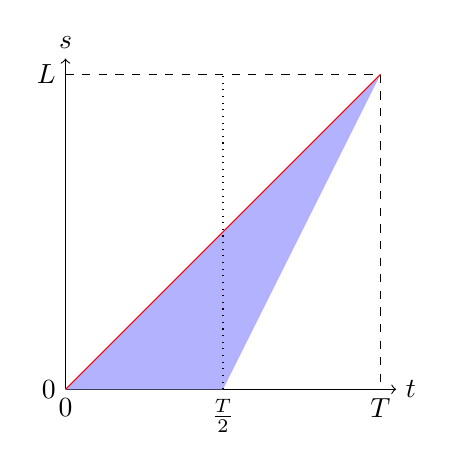
\begin{tikzpicture}[domain=0:4]
    \draw[->] (0,0) node[below] {0} -- (2,0) node[below] {$\frac{T}{2}$} -- (4,0) node[below] {$T$} -- (4.2,0) node[right] {$t$};
    \draw[->] (0,0) node[left] {0} -- (0,4) node[left] {$L$} -- (0,4.2) node[above] {$s$};
    \draw[dashed] (0,4) -- (4,4) -- (4,0);
    \fill[fill=blue!30] (0,0) -- (2,0) -- (4,4);
    \draw[dotted] (2,0) -- (2,4);
    \draw[color=red] plot (\x,\x);
  \end{tikzpicture}
\end{figure}


Tõenäosus, et auto sõidab jalgratturist mööda on võrdne sinise ala suhetega kogu pindalasse.
$$\frac{(L\times \frac T2)/2}{L \times T} = \frac{1}{4} \quad \pp{6}$$

Alternatiivselt saab vastuse leida ka ilma jooniseta. Sellisel juhul anda punkte arvutuste eest järgnevalt. Tõenäosus, et auto alustab sõitu jalgratturist eespool on $\frac{1}{2}$ \pp{2}. Tõenäosus, et auto alustab sõitu jalgratturist tagapool ja ei möödu jalgratturist on $\frac{1}{4}$ \pp{3}. Seega tõenäosus, et auto sõidab jalgratturist mööda on  $\frac{1}{4}$ \pp{1}.
\probend
\bigskip

% L105
\setAuthor{Krister Kasemaa}
\setRound{lõppvoor}
\setYear{2021}
\setNumber{G 6}
\setDifficulty{6}
\setTopic{TODO}

\prob{Keha keral}
\solu
\osa Vaatleme keha liikumist ümber $\theta$ defineeritud ringjoone. Laiuskraadil $\theta$ avaldub väikese keha tiirlemisraadius kujul
\[
  r=R \: \cos \theta
\]
ja joonkiirus kujul
\[
  v= \omega r= \frac{2 \pi }{T} r = \frac{2 \pi R \: \cos \theta}{T}.
\]
Nüüd saab avaldada tsentrifugaaljõu:
\[
  F_{\mathrm{ kesk}}=\frac{m v^2}{r} =\frac{m \left(\frac{2 \pi R \: \cos \theta}{T}\right)^2}{R \: \cos \theta}=\frac{4 m \pi^2 R \: \cos \theta}{T^2}.
\]
Arvestades, et kaalule panustab ainult radiaalne tsentrifugaaljõu komponent
\[
  F_{\mathrm{\bot kesk}}= \cos \theta \; F_{\mathrm{ kesk}} = \frac{4 \pi^2 m R \: \cos ^2 \theta}{T^2},
\]
saab leida keha kaalu:
\[
  W=\frac{G m M}{R^2} - \frac{4 \pi^2 m R \: \cos ^2 \theta}{T^2} = m\bigg(\frac{G M T^2 - 4 \pi^2 R^3 \: \cos ^2 \theta }{R^2 T^2}\bigg).
\]
\osa Libisemist põhjustab tsentrifugaaljõu kera pinnaga tangentsiaalne komponent:
\[
  F_{\mathrm{kesk || }}= \sin(|\theta|) \; F_{\mathrm{ kesk}} = \frac{4 \pi^2 m R \: \cos \theta \sin(|\theta|)}{T^2}=\frac{2 \pi^2 m R \: \sin(|2\theta|)}{T^2} .
\]
Hõõrdeõud avaldub kujul
\[
  F_{\mathrm{h}}=\mu W = \mu \, m\left(\frac{G M T^2 - 4 \pi^2 R^3 \: \cos ^2 \theta }{R^2 T^2}\right).
\]
Seega, tasakaalu korral:
\[
  F_{\mathrm{kesk || }} \leq \mu W,
\]
\[
  \frac{2 \pi^2 m R \: \sin(|2\theta|)}{T^2} \leq
  \mu \, m\bigg(\frac{G M T^2 - 4 \pi^2 R^3 \: \cos ^2 \theta }{R^2 T^2}\bigg)
\]
ja järelikult
\[
  \mu \geq \frac{2 \pi^2 R^3 \: \sin(|2\theta|)}{G M T^2 - 4 \pi^2 R^3 \: \cos ^2 \theta }.
\]
\probend
\bigskip

% L106
\setAuthor{Jaan Kalda}
\setRound{lahtine}
\setYear{2022}
\setNumber{G 6}
\setDifficulty{6}
\setTopic{TODO}

\prob{Saun}
\solu
Lahendus. Graafiku abil leiame veeauru osarõhu enne leili viskamist $p_a=\SI{1.2}{kPa}$. Ideaalse gaasi olekuvõrrandi abil leiame lisandunud aururõhu $p_bV=\frac m\mu RT$, millest $p_b=\frac {mRT}{\mu V}=\approx \SI{3.4}{kPa}$. Seega veeauru kogurõhk peale leili viskamist $p=p_a+p_b=\SI{4.6}{kPa}$; graafiku abil leiame sellele vastava kastepunkti väärtuse $t_k\approx \SI{32}\celsius$.
\probend
\bigskip

% L107
\setAuthor{Päivo Simson}
\setRound{piirkonnavoor}
\setYear{2022}
\setNumber{G 6}
\setDifficulty{6}
\setTopic{TODO}

\prob{Doomino}
\solu
\begin{equation*}
\tau=\frac{d}{u}. \qquad \p1
\end{equation*}
Sellel hetkel peab kuulike olema kõrgemal kui doominoklotsi kõrgus $h$, et mitte klotsi ümber lükata. Vähimale kiirusele vastab pikim võimalik liikumise aeg \p1. On selge, et selleks peab kuulike pärast põrget uuesti tõusma kõrgusele $H$ ja seejärel langema klotsini jõudmise hetkeks mitte madalamale kui $h$ \p1. Kõrguselt $H$ kukkumise aja $t_1$ saame leida seosest $H=gt_1^2/2$, mis annab
\begin{equation*}
t_1=\sqrt{\frac{2H}{g}}. \qquad \p1
\end{equation*}
Sama aeg kulub ka pärast põrget uuesti kõrgusele $H$ tõusmiseks. Kõrguselt $H$ kõrgusele $h$ langemiseks kulub aeg
\begin{equation*}
t_2=\sqrt{\frac{2(H-h)}{g}}. \qquad \p1
\end{equation*}
Kokku kulub klotsi ülemise servani jõudmiseks aeg $2t_1+t_2=\tau=d/u$ \p1. Siit saame pärast lihtsustamist minimaalseks kiiruseks
\begin{equation*}
  u=\frac{d\sqrt{g}}{2\sqrt{2H}+\sqrt{2(H-h)}}. \qquad \p1
\end{equation*}
\probend
\bigskip

% L108
\setAuthor{Jaan Kalda}
\setRound{lõppvoor}
\setYear{2022}
\setNumber{G 6}
\setDifficulty{6}
\setTopic{TODO}

\prob{Õhupüss}
\solu
\
Torus toimub gaasi adiabaatiline paisumine, kusjuures sõltumata toru pikkusest omandab gaas torus pärast kuuli välja lendamist toas valitseva õhurõhu. Seega on jäävad suurused nii $pV^\gamma$ kui $pV/T$, millest saame, et jääv suurus on ka $p^{\gamma-1}/T^\gamma$. Siit saame juba avaldada küsitud temperatuuri:
$$
T_1=T_0(p_0/p_1)^{\frac{\gamma - 1}{\gamma}}=T_0(p_0/p_1)^{2/7} \approx \SI{55}{\kelvin} \approx \SI{-218}{\celsius}
$$
\textit{Märkus:} tulemus on väiksem lämmastiku keemistemperatuurist, seega tegelikult langeb lämmastiku temperatuur keemistemperatuurini $\SI{-196}{\celsius}$ ning edasise paisumise juures püsib see konstantsena tänu vabanevale aurustumissoojusele.
\textit{PS:} adiabaadinäitaja on ka leitav valemiga $\gamma=c_P/c_V=(c_V+R)/c_V=1.4$.
\probend
\bigskip

% L109
\setAuthor{Marten Rannut}
\setRound{lahtine}
\setYear{2023}
\setNumber{G 6}
\setDifficulty{6}
\setTopic{TODO}

\prob{Võimas mootor}
\solu
Arvutame, mitu põlemistakti $N$ toimub mootoris 1 minuti jooksul. 4-taktilise mootori silindris toimub põlemistakt iga teine pööre ehk peame lisama konstandi $1/2$
$N = 1/2\cdot f n = 1/2\cdot \SI{8000}{\per\minute}\cdot 4= 16000$\\
Tulenevalt ideaalgaasi seadusest $V \cdot p = \frac{m}{\mu}RT$ (kus $V$ on gaasi ruumala, $p$ rõhk $m$ mass, $\mu$ molaarmass, $R$ universaalne gaasikonstant ja $T$ temperatuur) on gaasi tihedus $\frac{m}{V} = \frac{p\mu}{RT}$. Seega, kui gaasi tihedus temperatuuril $T_1$ on $\rho$, siis gaasi isobaarilisel soojendamisel temperatuurile $T_2$ muutub selle tihedus vastavalt valemile $\rho_2 = \rho \frac{T_1}{T_2}$. \\
Arvutame palju kütust $m$ põletab 1 põlemistakt, kui silindri maht on $v$.
$m = \rho_2v /\gamma  = \rho \frac{T_1}{T_2}v /\gamma  = \SI{1,2}{\gram\per\liter} \frac{\SI{293}{\kelvin}}{\SI{333}{\kelvin}} \SI{0,5}{\liter} / 14,7 \frac{g}{g} = \SI{0,036}{\gram}$

Kogu põletatud kütuse mass $M = N\cdot m = \SI{0,036}{\gram} * 16000 = \SI{576}{\gram}$

Arvutame mootori võimsuse  
$M \epsilon \eta \frac{1}{\SI{60}{\second}} = \SI{576}{\gram}\cdot\SI{46}{\kilo\joule\per\gram}\cdot 0,37\cdot \frac{1}{\SI{60}{\second}}=\SI{163}{\kilo\watt}$ 

Päris K20A mootori võimsus ongi umbes 162-165 kW olenevalt variandist.
\probend
\bigskip

% L110
\setAuthor{Erkki Tempel}
\setRound{piirkonnavoor}
\setYear{2023}
\setNumber{G 6}
\setDifficulty{6}
\setTopic{TODO}

\prob{Klaasplaat}
\solu
\begin{center}
\includegraphics[width=0.5\linewidth]{2023-v2g-06-yl.pdf}
\end{center}
  
Kolmnurgast $\triangle{ABC}$ saame avaldada kiire nihke $BC$\\
\[ BC = AC \cos{\alpha} \quad \p{2}\]

Külje $AC$ pikkuse saame leida lõikude $AD$ ja $CD$ kaudu
\[ AC = AD - CD  \quad \p{1}\]

Avaldame külje AD kolmnurgast $\triangle{ADE}$
\[ AD = d\tan{\alpha} \quad \p{1}\]
Külje CD leidmiseks kasutame murdumisnäitaja seost
\[ \frac{\sin{\alpha}}{\sin{\gamma}} = n \quad \Longrightarrow \quad \sin{\gamma} = \frac{\sin{\alpha}}{n} \quad   \p{1}\]
Kolmnurgast  $\triangle{CDE}$ saame avaldada $\sin{\gamma}$ ning sealt külje $CD$
\[ \sin{\gamma} = \frac{CD}{CE} \quad \Longrightarrow \quad  CD = \frac{CE \sin{\alpha}}{n} \quad\p{1}\]

Kasutades eelnevat seost ning Phytagorase teoreemi kolmnurgast $\triangle{CDE}$,
saame avaldada külje CD
\[  CD = \frac{d\sin{\alpha}}{\sqrt{n^2-\sin^2{\alpha}}} \quad \p{2}  \]

Seega nihkub esialgne kiir kõrvale oma algsest sihist 

\[ BC = d\sin{\alpha}\left(1 - \frac{\cos{\alpha}}{\sqrt{n^2-\sin^2{\alpha}}}\right)  \quad \p{2}  \]

Kui lõppvastusesse on jäetud lihtsustamata trigonomeetriline pöördfunktsioon (nt $\arcsin$, $\arccos$), siis anda ülesande eest kuni \p{8}.
\probend
\bigskip

% L111
\setAuthor{Martne Rannut}
\setRound{lõppvoor}
\setYear{2023}
\setNumber{G 6}
\setDifficulty{6}
\setTopic{TODO}

\prob{Nõel vees}
\solu
\par
Ülesandes kirjeldatud olukord on ligikaudu näidatud joonisel. Veepind pisut kõverdub ning seeläbi pindpinevusjõuga tasakaalustab nõela raskusjõu. Pindpinevusjõud mõjub veepinna sihis kontaktpunktides (see ei pruugi olla tangentsiaalne nõela pinnaga nagu on joonisel näidatud, kuid ülesande lahendust see ei mõjuta). Kummalegi poolele nõelast mõjub jõud $\sigma \ell$. Kui pindpinevusjõu vektorid on horisontaali suhtes nurga $\alpha$ all, siis saame jõudude tasakaalust \(mg = 2 \sigma \ell \sin \alpha\). Kuna veepind on sama nurga all kui jõuvektorid, siis otsitav nurk on
\[
\alpha = \arcsin{\frac{mg}{2\sigma \ell}} \approx \SI{34}{\degree}.
\]
\begin{center}
  \includegraphics[width=9cm]{2023-v3g-06-yl.pdf}
\end{center}
\probend
\bigskip

% L112
\setAuthor{Jaan Kalda}
\setRound{lahtine}
\setYear{2024}
\setNumber{G 6}
\setDifficulty{6}
\setTopic{TODO}

\prob{Vari}
\solu
\begin{figure}[h]
    \centering
    \includegraphics[width=.7\linewidth]{2024-lahg-06-yl.pdf}
\end{figure}

Lambi projektsiooni lauapinnale leiame kui ülaltvaates kera ja varju puutujate lõikepunkti $A$ (vt joonist). Tõmbame nüüd ringil horisontaalse puutuja ja vaatleme seda kui lauapinna vertikaallõike joont. Tõmbame varjule vertikaalpuutuja, selle lõikepunkt $C$ vasttõmmatud horisontaaljoonega on varju kaugeima punkti asukoht vaadeldaval vertikaallõikel. Tõmbame punktist $C$ puutuja ringjoonele ja punktist $A$ vertikaaljoone; nende lõikepunkt $B$ on lambi asukoht vertikaallõikel. Lambi kaugus vastab lõigule $OB$, joonlauaga mõõtes leiame, et see on umbes \SI{3.7}{} korda suurem, kui kera raadius.
\probend
\bigskip

% L113
\setAuthor{Päivo Simson}
\setRound{piirkonnavoor}
\setYear{2024}
\setNumber{G 6}
\setDifficulty{6}
\setTopic{TODO}

\prob{Mitteelastne nöör}
\solu
\begin{wrapfigure}{r}{0.5\textwidth}
  \vspace{-1em}
  \begin{center}
    \includegraphics[width=1\linewidth]{2024-v2g-06-yl1.pdf}
  \end{center}
  \vspace{-1em}
\end{wrapfigure}

Kuulike langeb kõigepealt vabalt kõrguse $h_0=\sqrt{l^2-a^2}$ võrra ja saavutab punktis $A$ kiiruse $v_0=\sqrt{2gh_0}$. Selleks hetkeks on nöör sirge ja toimub löök, mille korral tagasipõrget ei toimu, sest nöör on mitteelastne. Löögi käigus kaotab kuulike nöörisihilise kiiruse $\Vec{v}_0$ komponendi ja seega ka osa energiast (kaotatud energia läheb nöörile, mis selle arvelt soeneb). Kuulike jätkab liikumist mööda pikkusega $l$ määratud ringjoone kaart. Säilib ainult kiiruse komponent $v_1$, mis on paralleelne ringjoone puutujaga punktis A: $v_1=v_0\sin\alpha=v_0a/l=\sqrt{2gh_0}\,a/l$. Seega on kuulikese koguenergia vahetult pärast punkti A jõudmist
\[E = \frac{mv_1^2}{2}+mg(l-h_0)=mgh_0\frac{a^2}{l^2}+mg(l-h_0)=\]
\[=mgl\left(1-\frac{h_0}{l}\left(1-\frac{a^2}{l^2}\right)\right)=mgl\left(1-\left(1-\frac{a^2}{l^2}\right)^{\frac{3}{2}}\right).\]
Vabalangemisele järgnevalt jääb kuulike mööda ringjoone kaart võnkuma. Trajektoori kõrgeimas punktis on kuulikese kiirus null ja koguenergia on järelikult $E=mgH$, kus $H$ on otsitav maksimaalne kõrgus. Võrdsustades koguenergia avaldised saame
\[H=l\left(1-\left(1-\frac{a^2}{l^2}\right)^{\frac{3}{2}}\right).\]

\begin{wrapfigure}{r}{0.5\textwidth}
\vspace{-1cm}
  \begin{center}
    \includegraphics[width=1\linewidth]{2024-v2g-06-yl2.pdf}
  \end{center}
  \vspace{-1.0cm}
\end{wrapfigure}

Trajektoori joonestamiseks võrdleme kõrgusi $H$ ja $l-h_0$. Et $1-a^2/l^2=h_0^2/l^2$ ja $h_0/l<1$, siis
$l(1-h_0^3/l^3)>l(1-h_0/l)$
ehk $H>l-h_0$.
Kuuli trajektoor on näidatud parempoolsel joonisel paksu pideva joonega. Võrratuse $H>l-h_0$ näitamiseks piisab ka tähelepanekust, et punktis $A$, pärast löögi toimumist, on pallil endiselt kineetiline energia olemas ja seega ei saa punkt $A$ olla edasise liikumise kõrgeim punkt.
\probend
\bigskip

% L114
\setAuthor{Uku Andreas Reigo}
\setRound{lõppvoor}
\setYear{2024}
\setNumber{G 6}
\setDifficulty{6}
\setTopic{TODO}

\prob{Jahtumine}
\solu
Vedelik kaotab aja $t$ jooksul jahtudes soojushulga $Q$, mis on võrdeline jahutatava pindala $S$ ja temperatuuride vahega $\Delta T$: $Q = \propto  t S \Delta T$. Kuna eeldame, et tihedus ja erisoojus ei sõltu temperatuurist, siis vedeliku temperatuuri langemise kiirus $\dot{T}$ on võrdeline ajaühukus kaotatud soojushulgaga ja pöördvõrdeline vedeliku ruumalaga $V$:
\[
\dot{T} \propto \frac{Q}{Vt} \propto \frac{S \Delta T}{V}.
\]

Leiame soojema kokku valatud vedeliku temperatuuri $T_\text{segu}$ pärast soojusliku tasakaalu saabumist. Kuna kokku segatakse võrdsed kogused vedelikke, kehtib $T_\text{segu}-T = T_\text{lisa}-T_\text{segu}$, millest
\[
  T_\text{segu} = \frac{T+T_\text{lisa}}{2} = \frac{\SI{40}{\celsius}+\SI{88}{\celsius}}{2}=\SI{64}{\celsius}.
  \]

Kahe termose vedelikuga täidetud osad on sarnased koonused. Seega on nende täidetud ruumalad on proportsionaalsed kõrguse kuubiga ning põhjapindalad kõrguse ruuduga. Seega $S_2/S_1=h_2^2/h_1^2$ ja $V_2/V_1=h_2^3/h_1^3$, millest
\[
  \frac{S_2}{S_1}=\left(\frac{V_2}{V_1}\right)^{\frac{2}{3}} = \sqrt[3]{4}.
\]

Vedelike jahtumise suhe
\begin{align*}
  k &= \frac{\dot{T_2}}{\dot{T_1}} \\
  &= \frac{S_2}{S_1} \frac{V_1}{V_2} \frac{T_\text{segu} - T_\text{õhk}}{T - T_\text{õhk}} \\
    &= \frac{1}{\sqrt[3]{2}}\frac{T_\text{segu} - T_\text{õhk}}{T - T_\text{õhk}}.
\end{align*}
Millest
\[
    T_{õhk} = \frac{k T - \frac{T_\text{segu}}{\sqrt[3]{2}}}{k - \frac{1}{\sqrt[3]{2}}} = \frac{\num{1.62} \cdot \SI{40}{\celsius} - \frac{\SI{64}{\celsius}}{\sqrt[3]{2}}}{\num{1.62} - 1/\sqrt[3]{2}} = \SI{17}{\celsius}.
\]
\probend
\bigskip

% L115
\setAuthor{Krister Kasemaa}
\setRound{lahtine}
\setYear{2018}
\setNumber{G 7}
\setDifficulty{7}
\setTopic{TODO}

\prob{Kauss veega}
\solu
Käsitleme esmalt jõudu mida põhjustab veesamba impulsi muut kausile, jättes kõrvale veesamba massi mis langeb kaussi peale valamise lõppemist. Veesammas mõjub kausi põhjale jõuga $F=\frac{dp}{dt}$. Olgu vee kiirus vahetult enne põhja vastu põrkumist $v$. Võime teha lihtsustuse, et kausi põhja vastu põrkudes jääb vesi seisma. Seega,
\[
F=\frac{\mathrm{d}{p}}{\mathrm{d}{t}}=\frac{\mathrm{d}{m}}{\mathrm{d}{t}} |v|.
\]\par 
\noindent Järgmiseks leiame vee kiiruse vahetult enne kaussi jõudmist.  Valamise algushetkel on vee kiirus $v_0\approx 0$. Langedes rakendab veesambale jõudu ainult gravitatsioon. Seega rakendame valemit $v^2-v_0^2=2a\Delta s$, millest avaldub, et $v=\sqrt{2hg}$
Järelikult $F=\frac{\mathrm{d}{m}}{\mathrm{d}{t}} |v|=\frac{\mathrm{d}{m}}{\mathrm{d}{t}}\sqrt{2gh}$
Vee valamine lõpetati hetkel, kui $m_{\mathrm{kausis}} g+F=m_\mathrm{skaalal}g$, millest avaldub, et vee mass valamise hetkel kausis oli:
\begin{equation*}
m_{\mathrm{kausis}}=\frac{m_{\mathrm{skaalal}} g-F}{g}=m_{\mathrm{skaalal}}-\frac{\mathrm{d}{m}}{\mathrm{d}{t}}\sqrt{\frac{2h}{g}}.
\end{equation*}
Käsitleme nüüd veesamba massi, mis lisandub kaussi peale valamise lõppemist. Veesamba mass on $m_{\mathrm{veesammas}}=\frac{\mathrm{d}{m}}{\mathrm{d}{t}}\Delta t$, kus $\Delta t$ on aeg mil kulub veesamba ühe elementaarelemendi jõudmiseks kaussi. Rakendame valemit$v=v_0+at$ ja leiame, et:
\begin{equation*}
\Delta t = \frac{v-v_0}{g}=\frac{v}{g}=\sqrt{\frac{2h}{g}}.
\end{equation*}
Millest järeldub, et valamise lõppedes on kaussi jõudva veesamba mass on
\begin{equation*}
m_{\mathrm{veesammas}}=\frac{\mathrm{d}{m}}{\mathrm{d}{t}} \Delta t = \frac{\mathrm{d}{m}}{\mathrm{d}{t}}\sqrt{\frac{2h}{g}}.
\end{equation*}
Nüüd saame leida vee massi $M$, mis jõuab kaussi:
\begin{equation*}
M=m_{\mathrm{kausis}}+m_{\mathrm{veesammas}}=m_{\mathrm{skaalal}}-\frac{\mathrm{d}{m}}{\mathrm{d}{t}}\sqrt{\frac{2h}{g}}+\frac{\mathrm{d}{m}}{\mathrm{d}{t}}\sqrt{\frac{2h}{g}}=m_{\mathrm{skaalal}}.
\end{equation*}
\probend
\bigskip

% L116
\setAuthor{Jaan Kalda}
\setRound{lahtine}
\setYear{2019}
\setNumber{G 7}
\setDifficulty{7}
\setTopic{TODO}

\prob{Niit relssidel}
\solu
Olgu alumise rõnga kaugus nurgast $x$ ja vertikaalse rõnga kaugus $y$, niidi pikkus $L$ ja kinnituspunkti kõrgus $h$. Sellisel juhul $x^2+y^2=(L+y-h)^2$, võttes siit ajalise tuletise saame $2x\dot x+2y\dot y=2(L+y-h)\dot y$, kus punkt sümboli kohal tähistab ajalist tuletist, st $\dot x=v$. Lihtsustades seda avaldist leiame $vx=(L-h)\dot y$. Esiteks saame siit avaldada otsitava kiiruse
$$
\dot y=vx/(L-h)=v\left(\frac{L+y-h}{x-\frac yx}\right)^{-1}=
$$
$$
=v/(\frac 1{\cos\alpha}-\tan\alpha)^{-1}=\frac{v\cos\alpha}{1-\sin\alpha}.
$$
Teiseks, kui võtame antud avaldisest veelkord tuletise, saame $v\dot x=(L-h)\ddot y$, millest kiirendus $\ddot y=v^2/(L-h)$. Pangem tähele, et kiirendus püsib konstantne.
\probend
\bigskip

% L117
\setAuthor{}
\setRound{piirkonnavoor}
\setYear{2019}
\setNumber{G 7}
\setDifficulty{7}
\setTopic{TODO}

\prob{Lennurada}
\solu
Teame, et jõud on võrdeline õhu tiheduse ning kiiruse ruuduga. Seega olgu 
$$F=C\rho v^2 \Rightarrow v^2=\frac{F}{C\rho}$$
kus $C$ on võrdetegur. \pp{2} Kuna lennuk alustab hoovõttu paigalseisust ühtlase kiirendusega $a$, avaldub läbitud teepikkus $s=\frac{v^2}{2a}$. \pp{1} Kuna lennuki mass (ning seega ka õhkutõusuks vajaminev üleslükkejõud) ja kiirendus on mõlemal juhul samad \pp{1}, avalduvad teepikkused vastavalt:
$$s_1=\frac{v_1^2}{2a}=\frac{F}{2Ca\rho_1}\quad\pp{1}$$ 
$$s_2=\frac{v_2^2}{2a}=\frac{F}{2Ca\rho_2}\quad\pp{1}$$   

Võrrandid omavahel jagades saame:
$$\frac{s_1}{s_2}=\frac{\rho_2}{\rho_1}\quad\pp{1}$$ 
Siit saame avaldada vajaliku lennuraja pikkuse $s_2 = s_1\frac{\rho_1}{\rho_2} \approx \SI{3}{km}\quad  \pp{1}$.
\probend
\bigskip

% L118
\setAuthor{}
\setRound{lõppvoor}
\setYear{2019}
\setNumber{G 7}
\setDifficulty{7}
\setTopic{TODO}

\prob{3 ruutu}
\solu
Lihtsustame skeemi arvestades sellega, et ideaalsete ampermeetrite sisetakistus on null: me võime lühistada need sõlmpunktid, mis on ühendatud juhtmega läbi ampermeetri. Selleks, et olla kindel vigadeta skeemi teisendamises tähistame takistid numbritega ja sõlmpunktid tähtedega, vt esimene joonis. Paneme tähele, et Kirchoffi vooluseaduse tõttu näitavad ampermeetrid vastavalt esimese ja viienda, seitsmenda ja neljanda ning kaheksanda ja neljanda  takisti voolude vahet.

Seejärel alustame sõlmpunktide märkimisest ja ühendame need samade takistitega, mis algseski skeemis, tulemus on näidatud teisel joonisel. Viimase sammuna  jagame sõlmpunkti C kaheks osaks lõigates mõtteliselt läbi joonise sümmeetriateljel oleva vertikaalse juhtme; seda võib teha,  sest sümmeetria tõttu puudub selles vertikaalses juhtmes vool. Nüüd on juba lihtne leida takistite voolud: takistitest 8 ja 9 koosneva ahela kogutakistus on $r_8=\SI {6}\ohm$, seetõttu  läbib neid vool $i_8=\mathcal E/r_8=\SI 8A$. Punktide B ja D vahelise viiest takistist koosneva ahelajupi takistus on $\frac 67\SI {}\ohm$ ning seega ülemise ahelapoole kogutakistus on $r_1=\frac {48}7\SI {}\ohm$ ja takisti 1 vool $i_1=\mathcal E/r_1=\SI 7A$. Seega langeb takistite 1 ja 7 peale kokku pinge $2i_1R=\SI {42}V$, mistõttu sõlmede B ja D vaheline pinge on $V_5=\mathcal E-2i_1R=\SI {6}V$. Järelikult on takisti 5 vool $i_5=V_5/R=\SI 2\A$ ja takisti 2 vool $i_2=V_5/(2R)=\SI 1\A$. 

Niisiis on vasakpoolse ülemise ampermeetri vool $i_8=i_1-i_5=\SI 5A$ ning sümmeetria tõttu näitab sama voolutugevust ka parempooolne ülemine
 
ampermeeter. Alumise ampermeetri näit on $i_8-i_2=\SI 7A$.\\

\begin{figure}[h]
    \centering
    \begin{subfigure}[h]{0.45\textwidth}
     \includegraphics[width=\textwidth]{2019-v3g-07-yl1.pdf}\\
    \end{subfigure}
    \begin{subfigure}[h]{0.45\textwidth}
    \vspace{-10pt}
     \includegraphics[width=\textwidth]{2019-v3g-07-yl2.pdf}
    \end{subfigure}
 \end{figure}
\probend
\bigskip

% L119
\setAuthor{Krister Kasemaa}
\setRound{lahtine}
\setYear{2020}
\setNumber{G 7}
\setDifficulty{7}
\setTopic{TODO}

\prob{Poolsilinder basseinis}
\solu
Vaatleme poolsilindrit ning selle kohal olevat veesammast ühtse kehana. Me saame seda teha, sest süsteem on tasakaalus ning vesi on paigal.
Paneme esmalt kirja jõudude tasakaalu vertikaalsihis.
Vertikaalsihis mõjub raskusjõud ning poolsilindri ja põranda vaheline toereaktsioon $N$.

Poolsilindri kohal oleva veesamba ruumala on
\begin{equation*}
	V_{\mathrm{vesi}}=l r^2-\pi \frac{r^2 l}{4}=l r^2\left(1-\frac{\pi}{4}\right).
\end{equation*}
Seega, vertikaalne jõudude tasakaal avaldub kujul
\begin{equation*}
	N=g(\rho V_{\mathrm{vesi}} + m) = g\left(\rho l r^2\left(1-\frac{\pi}{4}\right) + m\right).
\end{equation*}
Teades reaktsioonijõudu $N$ on lihtne leida hõõrdejõud poolsilindri ja põhja vahel:
\begin{equation*}
	F_{\mu}=\mu N= \mu g \left(\rho l r^2\left(1-\frac{\pi}{4}\right) + m\right).
\end{equation*} 
Horisontaalsuunas tasakaalustab hõõrdejõudu vee horisontaalsuunaline rõhumisjõud $F_{\mathrm{vedelik}}$. Poolsilindri ja selle kohal olevale veesamba süsteemile mõjub keskmiselt rõhk $p = \rho gr/2$, kusjuures kontaktpindala on $S = lr$. Järelikult on horisontaalsuunaline jõud
\begin{equation*}
	F_{\mathrm{vedelik}}=\frac{\rho g r}{2}r l=\frac{\rho g l r^2}{2} F_{\mu}.
\end{equation*}
Kombineerides mõlemad avaldised $F_\mu$ jaoks, saame
\begin{equation*}
	\mu_0=\frac{\rho l r^2}{2(\rho l r^2(1-\frac{\pi}{4})+m}.
\end{equation*}
\probend
\bigskip

% L120
\setAuthor{}
\setRound{piirkonnavoor}
\setYear{2020}
\setNumber{G 7}
\setDifficulty{7}
\setTopic{TODO}

\prob{Jälle sauna!}
\solu
Vesi keeb 100 kraadi juures ja tekkinud veeaur kaotab hea soojusliku kontakti kerisekividega ning seetõttu ei jõua oluliselt üle 100 kraadi kuumeneda. \pp{2} Niisiis võime eeldada, et $\nu_a=p_0V/RT_a\approx 341$ mooli õhku \pp{1} temperatuuril $T_a$ seguneb $\nu_w=m/\mu_w\approx 11$ mooli veeauruga \pp{1} temperatuuril $T_a+\Delta T$, kus $\Delta T=\SI {20}\celsius$ \pp{1}. Seega saame soojusbalansi kirja panna kujul $c_{pw}\nu_w(\Delta T-\delta T)=c_{pa}\nu_a\delta T$ \pp{2}, kus $\delta T$ tähistab õhutemperatuuri muutu ja $c_{pa}=c_a+R$ \pp{1} ning $c_{pw}=c_w+R$ \pp{1} tähistavad õhu ja veeauru molaarseid erisoojusi konstantsel rõhul. (Kasutada tuleb erisoojust konstantsel rõhul, sest kogu protsess toimub konstantse atmosfäärirõhu juures --- üleliigne õhk pääseb välja; kes kasutab $c_a$-d ja $c_w$-d jääb neist kahest punktist ilma.) Siit saame $\delta T=c_{pw}\nu_w\Delta/(c_{pw}\nu_w+c_{pa}\nu_a)\approx\SI{0.3}\celsius$ \pp{1}. Nagu näeme on temperatuuri muutus üsna väike, subjektiivselt hakkab palavam õhuniiskuse tõusu tõttu. Pikemas ajaskaalas leil jahutab kerisekive, mis ei kuumuta enam õhku endise võimsusega ja temperatuur võib hoopis langema hakata.
\probend
\bigskip

% L121
\setAuthor{}
\setRound{lõppvoor}
\setYear{2020}
\setNumber{G 7}
\setDifficulty{7}
\setTopic{TODO}

\prob{Pulgad}
\solu
\osa Olgu silindrile mõjuv normaaljõud kummaski punktis $N$ (puutujaga risti) ning hõõrdejõud $F_h$ (puutujaga paralleelne). Olgu nurk pulkade vahel $2\alpha$.

\begin{figure}[h]
\centering
\includegraphics[width=0.5\linewidth]{2020-v3g-07-yl.pdf}
\end{figure}

Jõudude tasakaalust saame, et puutepunktides mõjuvad resultantjõud $\vec N + \vec{F_h}$ peavad olema paralleelsed ja vastassuunalised, seega sümmeetria tõttu peab $\vec N + \vec{F_h}$ olema sümmeetriateljega risti.

Kuna puutuja on raadiusega risti, on lihtne näidata, et nurk $\vec N$ ja puutepunkte ühendava sirge vahel on $\alpha$, seega $\tan \alpha = \frac{F_h}{N}$. Piirjuhul, kus $\mu$ on minimaalne, $F_h = \mu N$ ja seega
$$\tan \alpha = \frac{\mu N}{N} = \mu$$

Teisalt $\tan \alpha = \frac{R}{L}$, seega
$$\mu_\text{min} = \frac{R}{L}$$

\osa Nagu eelmises osas näidatud, siis hõõrdejõu lauaga paralleelne komponent $F_{h,r} = N\tan \alpha = \frac{R}{L}\cdot N$. Silindrit üles tõstes peab raskusjõu tasakaalustamiseks lisaks mõjuma kummaski punktis hõõrdejõu lauaga risti olev komponent $F_{h,t} = \frac{mg}{2}$, seega kui summaarne hõõrdejõud on $F_h$, siis
$$F_h^2 = F_{h,r}^2 + F_{h,t}^2 = \frac{R^2}{L^2}N^2 + \frac{m^2g^2}{4}$$

Piirjuhul $F_h = \mu N$ ja $\tau = NL$, seega
$$\mu^2N^2 = \frac{R^2}{L^2}N^2 + \frac{m^2g^2}{4}$$
$$\left(\mu^2 - \frac{R^2}{L^2}\right)N^2 = \frac{m^2g^2}{4}$$
$$N = \frac{mg}{2\sqrt{\mu^2-\frac{R^2}{L^2}}}$$
$$\tau_\text{min} = NL = \frac{mgL}{2\sqrt{\mu^2-\frac{R^2}{L^2}}} = \frac{mgL^2}{2\sqrt{L^2\mu^2 - R^2}}$$
\probend
\bigskip

% L122
\setAuthor{Jaan Kalda}
\setRound{lahtine}
\setYear{2021}
\setNumber{G 7}
\setDifficulty{7}
\setTopic{TODO}

\prob{Hantel}
\solu
Hantli massikeskme kiirendus on $a=\frac{Eq}{2m}$. Kasutame süsteemi, mis liigub kiirendusega $\frac{Eq}{2m}$ ja kus hantli massikese on paigal. Selles süsteemis mõjub kummalegi kerale elektriväljale vastassuunaline inertsijõud $F=am=\frac{Eq}{2}$, st laenguga kerale mõjub elektrivälja suunaline resultantjõud $\frac{Eq}{2}$ ning laenguta kerale mõjub samasuur kuid vastassuunaline jõud. Nende jõudude potentsiaalse energia muutus (võrreldes algasendiga) on maksimaalne hetkel, kui hantel on pöördunud täisnurga võrra: $$\Delta E_p=2\cdot \frac{Eq}2\cdot\frac l2=\frac{Eql}2;$$ selles valemis arvestasime, et kummagi kera jõusihiline nihe on $\frac l 2$. Energia jäävusest tulenevalt on siis maksimaalne ka kineetiline energia ja nurkkiirus.  Seega saame energia jäävuse seadusest $$\frac{Eql}2=2\cdot \frac{mv^2}2,$$ kus $v$ on kummagi kuulikese kiirus meie taustsüsteemis antud ajahetkel. Järelikult $v=\sqrt{\frac{Eql}{2m}}$ ning otsitav nurkkiirus $$\omega=\frac{\sqrt{\frac{Eql}{2m}}}{\frac{l}{2}}=\sqrt{\frac{2Eq}{ml}}.$$
\probend
\bigskip

% L123
\setAuthor{Kaur Aare Saar}
\setRound{piirkonnavoor}
\setYear{2021}
\setNumber{G 7}
\setDifficulty{7}
\setTopic{TODO}

\prob{Rippuv laeng}
\solu
Selleks, et rippuv laeng püsiks paigal, peab talle mõjuvate jõuvektorite summa olema $0$. Rippuvale laengule mõjub kolm jõudu, raskusjõud $mg$, nööri pinge $T$ ning laengute vaheline elektrostaatiline jõud $F$. \pp1

\begin{figure}[H]
	\centering
	\begin{tikzpicture}[scale=1.5]
    \coordinate (A) at (0,0);
    \coordinate (q1) at (1,-2);
    \coordinate (q2) at (0,-4);
    \coordinate (D) at (1,-0);
    \coordinate (E) at (0.5,-1);
    \coordinate (F) at (1.5,-1);
    \coordinate (G) at (1,-4);

    % kinnitus
    \fill [pattern = north east lines] (-0.5,0) rectangle (0.5,0.2);
    \draw[thick] (-0.5,0) -- (0.5,0);

    %nöör
    \draw [thick] (q1)	-- (A) node[yshift=-1.2cm,xshift=0.9cm] {$L$};

    %abijooned
    \draw [dashed] (q2) -- (A) node[midway,left] {$2h$};
    \draw [dashed] (q1) -- (q2) node[midway, right] {$L$};
    \draw [dashed] (q1) -- (D) node[right,yshift=-1.2cm] {$h$};

    %jõud
    \draw[line width=2pt,blue,-stealth](q1)--(E) node[anchor=north east]{$T$};
    \draw[line width=2pt,blue,-stealth](q1)--(F) node[anchor=north west]{$F$};
    \draw[line width=2pt,blue,-stealth](q1)--(G) node[anchor=north west]{$mg$};

    %nurgad
    \draw pic [text="$\theta$", draw, angle radius=1.1cm] {angle=q2--A--q1};
    \draw pic [text="$\theta$", draw, angle radius=1.05cm] {angle=D--q1--A};
    \draw pic [text="$\theta$", draw, angle radius=1.1cm] {angle=F--q1--D};    

    %laengud
    \node[circle,fill=black,inner sep=1mm] at (q1) {};
    \node[circle,fill=black,inner sep=1mm] at (q2) {};
  \end{tikzpicture}
\end{figure}

Paneme tähele, et kinnituskoht, rippuv laeng ning fikseeritud laeng moodustavad võrdhaarse kolmnurga, mistõttu on laengute vaheline kaugus~$L$~\pp1.

Seega laengute vaheline elektrostaatiline jõud on:
$$F=\frac{kq_1q_2}{L^2} \quad \pp1$$

Raskusjõul puudub horisontaalkomponent. Järelikult on elektrostaatilise jõu ja nööri pinge horisontaalkomponendid võrdsed ja vastassuunalised \pp1.

Seega kuna elektrostaatilise jõu ja nööri pinge horisontaalkomponendid on võrdsed, siis sümmeetria tõttu on need jõud absoluutväärtuselt võrdsed $T=F$ \pp1.

Nüüd vertikaalsuunalisest jõudude tasakaalust saame
$$mg=T\cos\theta + F\cos (-\theta) = 2F\cos\theta = 2 \cos\theta \frac{kq_1q_2}{L^2} \quad \pp3,$$
kus $\theta$ on nurk vertikaalsihi ja nööri vahel.
Täisnurksest kolmnurgast saame $\cos\theta = \frac hL$ \pp1.

Nüüd asendades sisse $\cos\theta$ vertikaalsuunalise jõudude tasakaalu võrrandisse ja avaldades sealt $m$, saame
$$m=\frac{2kq_1q_2h}{gL^3} \quad \pp1$$
\probend
\bigskip

% L124
\setAuthor{Jaan Kalda}
\setRound{lõppvoor}
\setYear{2021}
\setNumber{G 7}
\setDifficulty{7}
\setTopic{TODO}

\prob{Kolmnurk}
\solu
Et osakesed liiguksid sirgjooneliselt, peaks see kolmnurk, mille tippudes need asuvad, jääma iseenesega sarnaseks. Et kolmnurga mediaanide lõikepunkt (massikese) jääb väliste jõudude puudumise tõttu paigale, siis peavad kõigile osakestele mõjuvad resultantjõud mõjuma piki mediaane ning nende moodulid peavad olema võrdelised vastavate mediaanide pikkustega (siis on mediaanide kasvamise kiiendused ja kiirused võrdelised mediaanide pikkustega ja kolmnurk jääb iseenesega sarnaseks).

Tähistame punktist $C$ lähtuvad küljed vektoritega $\vec a$ ja $\vec b$; tipust $C$ tõmmatud mediaan on $(\vec a+\vec b)/2$; sarnased avaldised saame ka ülejäänud mediaanide jaoks. Järelikult peavad osakestele mõjuvad resultantjõud avalduma kujul $p(\vec a+\vec b)=kq_C(\frac {\vec aq_B}{a^3}+\frac {\vec bq_A}{b^3})$, kus $p$ on konstant (sama kõigi osakeste jaoks kirjutatud avaldiste puhul) ning $k$ on Coulomb'i konstant. See võrdus kehtib ainult siis, kui $\frac {q_B}{a^3}=\frac {q_A}{b^3}$, st $q_Bb^3=q_Aa^3$. Analoogselt leiame, et  $q_Cc^3=q_Aa^3$, st $q_Aa^3=q_Bb^3=q_Cc^3\equiv Q$.

Kasutades siindefineeritud suurust  $Q$ saame avaldada konstandi $p=\frac {kQ}{a^3b^3c^3}$; sümmeetria tõttu on ilmne, et teiste osakeste jaoks saame täpselt samasuguse avaldise, nii nagu vajalik osakeste sirgjooneliseks liikumiseks. Seega: jah, iga kolmnurga puhul on võimalik osakeste sirgjooneline liikumine, vajalik on vaid rahuldada võrdus $q_Aa^3=q_Bb^3=q_Cc^3$.
\probend
\bigskip

% L125
\setAuthor{Jaan Kalda}
\setRound{lahtine}
\setYear{2022}
\setNumber{G 7}
\setDifficulty{7}
\setTopic{TODO}

\prob{Elektron ja kondensaator}
\solu
Lahendus. Optimaalne trajektoor on selline, mis riivab ühte plaati kondensaatori keskpunkti juures ja väljub vastasplaati riivates. Et $d\ll b$, siis on sisenemis- ja väljumisnurgad väiksed ning me võime lugeda, et elektroni plaadisihiline kiiruskomponent (mis püsib konstantsena, sest elekrivälja jõud on sellega risti) on võrdne $v$-ga. Elektroni liikumine on samasugune, nagu pallil Maa raskusväljas. Elektron viibib plaatide vahel aja $t=b/v$; et elektroni kiirendus $a=Ee/m$, siis saame välja kirjutada tingimuse, et elektron jõub ühe plaadi keskpunkti juurest startides liikuda plaatide ristsihis vahemaa $$d=\frac a2\left(\frac t2\right)^2=\frac{Eeb^2}{8v^2m}.$$ Arvestades, et $E=U/d$ saame siis avaldada $$v=\frac b{2d}\sqrt{\frac{Ue}{2m}}.$$
\probend
\bigskip

% L126
\setAuthor{Taavet Kalda}
\setRound{piirkonnavoor}
\setYear{2022}
\setNumber{G 7}
\setDifficulty{7}
\setTopic{TODO}

\prob{Plastiliin}
\solu
Peale esimest kokkupõrget nihkub plaadi tasakaaluasend $mg/k$ võrra allapoole ning plaat hakkab uue tasakaaluasendi ümber teatud amplituudiga võnkuma (amplituudi väärtust pole punktide saamiseks vaja leida) \p3. Kuna plaadi mass on plastiliini massiga võrreldes tühine, omandab plaat kokkupõrke hetkel impulsi jäävuse tõttu sama kiiruse nagu plastiliin, seega plaadi kiirus on energia jäävusest $v_0 = \sqrt{2gh}$ ($v_0$ avaldist pole punktide saamiseks vaja leida). Energia jäävusest järeldame, et plaadi kiirus on samuti $v_0$ siis, kui teine plastiliinitükk plaadiga kontakti loob \p2. See tuleneb asjaolust et plaadi kõrgus lauast, ehk teisisõnu plaadi potentsiaalne energia, on hetk enne teist kokkupõrget sama mis see oli just peale esimest kokkupõrget. Seega on teise plastiliini kokkupõrge plaadiga efektiivselt sama kui kahe identse massi ja kiirusega objektide lauskokkupõrge. Seega jääb plaat peale teist kokkupõrget seisma \p2. Samas nihkub plaadi tasakaaluasend veel $mg/k$ võrra allapoole ning plaat hakkab amplituudiga $2mg/k$ uue tasakaaluasendi ümber võnkuma \p2. Seega on järgneva liikumise käigus plaadi kõige alumine asend $4mg/k$ võrra esialgsest asendist all pool \p1.
\probend
\bigskip

% L127
\setAuthor{Oleg Košik}
\setRound{lõppvoor}
\setYear{2022}
\setNumber{G 7}
\setDifficulty{7}
\setTopic{TODO}

\prob{Veeuputus}
\solu
\
Paneme tähele, et \SI{1}{l\per m^2}=\SI{1}{mm} ehk otsitav torustiku äravool on arvuliselt võrdne äraveetavate sademete hulgaga millimeetrites.

Olgu $h_6=\SI{22}{\mm}$ sademete koguhulk 6 minuti järel ning $h_9=\SI{28}{\mm}$ omakorda 9 minuti järel, $H$ mitu millimeetrit sademeid suudab endas mahutada kraav (kui äravoolu ei oleks) ning $u$ töökorras torustiku sademete äravoolu kiirus millimeetrites minutis.

Saame võrrandid
\[
h_6 = H +0.5 u \cdot \SI{6}{\min}
\]
ja
\[
h_9 = H + u \cdot \SI{9}{\min}
\]
Sellest võrrandisüsteemist leiame $H=\SI{19}{\mm}$.

Olgu otsitud äravoolu kiirus $u_x$. Siis sirge $h(t)=H+u_xt$ näitab, kui palju suudab kanalisatsioonisüsteem akumuleerida vett maksimaalselt igal ajahetkel ($H$ on kraavi panus $u_xt$ sadeveetorustiku panus). Selleks, et uputus ei tekiks, peab sademete koguhulga graafik jääma alati sellest sirgest allapoole. Kiirus $u_x$ on minimaalne siis, kui see sirge on graafiku puutuja. Tõmbame niisiis graafikult puutuja, mis läbib punkti $(0,H)$. Selle puutuja tõus on otsitav kiirus $u_x$. Mõõtmised annavad meile $u_x=\SI{1.23}{mm/min}=\SI{1.23}{\L\per\m\squared}$ minutis.

\begin{figure}[h]
	\vspace{-1em}
    \centering
    \includegraphics[width=0.75\linewidth]{2022-v3g-07-yl.pdf}
\end{figure}
\probend
\bigskip

% L128
\setAuthor{Jaan Kalda}
\setRound{lahtine}
\setYear{2023}
\setNumber{G 7}
\setDifficulty{7}
\setTopic{TODO}

\prob{Soojuspump}
\solu
Oletame, et toa efektiivne soojusmahtuvus on $C$. Efektiivne soojusmahtuvus iseenesest ei pruugi olla üheselt mõistetav suurus, sest nt lühikese aja jooksul ei jõua seinte sügavamad osad veel soojeneda, mistõttu efektiivne soojusmahtuvus kasvab koos vaadeldava karakteerse ajavahemikuga. Antud juhul aga loodame, et karakteersed ajavahemikud --- $t_1$ ning hilisemas töörežiimis protsessi poolperiood --- tulevad samas suurusjärgus. Kui soojuspumba kütmisvõimsus on $P$, siis saame $Pt_1=C(T_1-T_0)$. Kui toa temperatuur on $T_f$, siis on ka soojuskadude võimsus $P_f$; üldjuhul on soojuskaod võrdelised sise- ja välistemperatuuride vahega, st soojuskadude võimsus $P_s=P(T-T_0)/(T_f-T_0)$. Nüüd saame välja kirjutada tingimused töörežiimis soojuspumba töötamise ($t_s$) ja puhkamise ($t_v$) ajavahemilke jaoks: $t_vP(T_k-T_0)/(T_f-T_0)=C(T_3-T_2)$ ning $t_s[P-P(T_k-T_0)/(T_f-T_0)]=t_sP(T_f-T_k)/(T_f-T_0)=C(T_3-T_2)$, kus $T_k=(T_3+T_2)/2=\SI{22}\celsius$ on toa keskmine temperatuur. Asendades $C$ esimesest võrrandist saame $$t_v=t_0\frac{T_3-T_2}{T_1-T_0}\frac{T_f-T_0}{T_k-T_0}=\SI{30}{\min}$$ ning $$t_s=t_0\frac{T_3-T_2}{T_1-T_0}\frac{T_f-T_0}{T_f-T_k}=\SI{30}\min.$$ Seega koguperiood $t_k=t_v+t_s=\SI{60}\min$.
\probend
\bigskip

% L129
\setAuthor{Päivo Simson}
\setRound{piirkonnavoor}
\setYear{2023}
\setNumber{G 7}
\setDifficulty{7}
\setTopic{TODO}

\prob{Voltmeeter}
\solu
Olgu voltmeetri sisetakistus $R_v$. Skeemi sümmeetriast ja võrdusest $V_{AB}=V_{CD}$ järeldub, et takistused $R_1$ ja $R_3$ peavad olema võrdsed, st $R_3=R_1$. \p{1}

\begin{wrapfigure}{r}{0.35\textwidth}
\vspace{-1em}
  \begin{center}
    \includegraphics[width=1\linewidth]{2023-v2g-07-yl1.pdf}
  \end{center}
\end{wrapfigure}

1) Koostame kõigepealt skeemi, mis kujutab pinge mõõtmist punktide A ja B vahel. $R_v$ ja $R_1$ on ühendatud rööbiti ja takistus punktide A ja B vahel on järelikult
\[
R_{AB}=\frac{R_v R_1}{R_v + R_1}. \quad \p{0,5}
\]
Skeemi kogutakistus on
\[
R_{k}=\frac{R_v R_1}{R_v + R_1} + R_1+R_2. \quad \p{0,5}
\]
Pinge kahe punkti vahel jaotub proportsionaalselt nende punktide vahelise takistusega ja järelikult
\begin{multline*}
V_{AB}=U\cdot\frac{R_{AB}}{R_k}=\frac{U\frac{R_v R_1}{R_v + R_1}}{\frac{R_v R_1}{R_v + R_1} + R_1+R_2}=\\
=\frac{UR_vR_1}{R_v(2R_1+R_2)+R_1(R_1+R_2)}. \quad \p{1}
\end{multline*}

\begin{wrapfigure}{r}{0.35\textwidth}
\vspace{-1em}
  \begin{center}
    \includegraphics[width=1\linewidth]{2023-v2g-07-yl2.pdf}
  \end{center}
\end{wrapfigure}

2) Koostame skeemi, mis kujutab pinge mõõtmist punktide A ja C vahel. Analoogiliselt eelmise skeemiga saame
\[
R_{AC}=\frac{R_v (R_1+R_2)}{R_v + R_1+R_2}, \quad \p{0,5}
\]
\[
R_{k}=\frac{R_v (R_1+R_2)}{R_v + R_1+R_2}+R_1, \quad \p{0,5}
\]
\begin{multline*}
V_{AC}=U\cdot\frac{R_{AC}}{R_k}=\frac{U\frac{R_v (R_1+R_2)}{R_v + R_1+R_2}}{\frac{R_v (R_1+R_2)}{R_v + R_1+R_2}+R_1}=\\
=\frac{UR_v(R_1+R_2)}{R_v(2R_1+R_2)+R_1(R_1+R_2)}. \quad \p{1}
\end{multline*}

3) Paneme tähele, et $V_{AB}$ ja $V_{AC}$ murdavaldiste nimetajad on samad. Jagame need avaldised omavahel.
\[
\frac{V_{AB}}{V_{AC}}=\frac{R_1}{R_1+R_2}=\frac{28}{84}=\frac{1}{3} \quad\implies\quad R_2=2R_1. \quad \p{2}
\]
Asendades saadud tulemuse $V_{AB}$ avaldisse saame
\[
\frac{126 R_v}{4R_v+3R_1}=28\quad\implies\quad R_v=6R_1. \quad \p{2}
\]

\begin{wrapfigure}{r}{0.35\textwidth}
\vspace{-2em}
  \begin{center}
    \includegraphics[width=1\linewidth]{2023-v2g-07-yl3.pdf}
  \end{center}
\vspace{-5em}
\end{wrapfigure}

4) Nüüd saame leida voltmeetri näidu $V_{BC}$. Vastavalt skeemile saame
\begin{multline*}
V_{AB}=U\cdot\frac{R_{BC}}{R_k}=\SI{126}{V}\cdot\frac{\frac{2R_1\cdot6R_1}{8R_1}}{\frac{2R_1\cdot6R_1}{8R_1}+2R_1}=\\
=\SI{126}{V}\cdot\frac{12}{12+8\cdot2}=\SI{54}{V}. \quad \p{1}
\end{multline*}
\probend
\bigskip

% L130
\setAuthor{Eero Vaher}
\setRound{lõppvoor}
\setYear{2023}
\setNumber{G 7}
\setDifficulty{7}
\setTopic{TODO}

\prob{Tehiskaaslane}
\solu
\par
Paneme tähele, et orbiidi kaugeimas punktis peab tehiskaaslase kiirusvektori projektsioon tehiskaaslast planeedi keskmega ühendavale lõigule olema $0$. Kui kiirusvektori projektsioon oleks positiivne, liiguks tehiskaaslane planeedist eemale ning tehiskaaslane oleks järgmisel ajahetkel planeedist kaugemal. Kui kiirusvektori projektsioon oleks negatiivne, oleks tehiskaaslane planeedile lähemale liikumas ning tehiskaaslane olnuks eelmisel ajahetkel planeedist kaugemal.

Ringorbiidil oleva keha jaoks on kesktõmbejõuks gravitatsioonijõud ehk $\frac{mv^2}{r}=\frac{GMm}{r^2}$, kus $G$ on gravitatsioonikonstant, $M$ planeedi ning $m$ tehiskaaslase mass. Järelikult $GM=v^2r$.

Vaatleme esmalt juhtu, kus tehiskaaslasele antaks kiirendus selle liikumissuunas. Vahetult pärast kiirenduse saamist oleks tehiskaaslase kiirus $u_1=v+\Delta v=\frac{31}{24}v$. Selle koguenergia oleks $E_1=\frac{mu_1^2}{2}-\frac{GMm}{r}$ ning selle impulsimoment $L_1=mru_1$. Olgu tehiskaaslase kiirus orbiidi kaugeimas punktis $w_1$. Impulsimomendi jäävuse põhjal $L_1=mR_1w_1$ ehk $w_1=\frac{r}{R_1}u_1$ ning energia jäävuse põhjal $E_1=\frac{mw_1^2}{2}-\frac{GMm}{R_1}$ ehk $\frac{u_1^2}{2}-v^2=\frac{u_1^2r^2}{2R_1^2}-\frac{v^2r}{R_1}$. Selle saame teisendada kujule $\left(\frac{u_1^2}{2}-v^2\right)R_1^2+v^2rR_1-\frac{u_1^2r^2}{2}=0$. Selle võrrandi lahendid on $R_1=\frac{-v^2r\pm\sqrt{v^4r^2-2v^2u_1^2r^2+u_1^4r^2}}{u_1^2-2v^2}=\frac{-v^2r\pm\sqrt{\left(1-2\left(\frac{31}{24}\right)^2+\left(\frac{31}{24}\right)^4\right)v^4r^2}}{\left(\frac{961}{576}-2\right)v^2}=\frac{1\mp\left(\frac{961}{576}-1\right)}{\frac{191}{576}}r$. Suurim kaugus oleks järelikult $R_1=\frac{961}{191}r=\SI{277729}{km}$.

Kui kiirendus oleks suunatud planeedist eemale, oleks tehiskaaslase kiirus vahetult pärast kiirenduse saamist $u_2=\sqrt{v^2+\Delta v^2}=\frac{25}{24}v$. Selle koguenergia oleks $E_2=\frac{mu_2^2}{2}-\frac{GMm}{r}$ ning impulsimoment $L_2=mrv$. Olgu tehiskaaslase kiirus orbiidi kaugeimas punktis seekord $w_2$. Impulsimomendi jäävuse põhjal $L_2=mR_2w_2$ ehk $w_2=\frac{r}{R_2}v$ ning energia jäävuse põhjal $\frac{u_2^2}{2}-v^2=\frac{v^2r^2}{2R_2^2}-\frac{v^2r}{R_2}$ ehk $\left(\frac{u_2^2}{2}-v^2\right)R_2^2+v^2rR_2-\frac{v^2r^2}{2}=0$, mille lahendid on $R_2=\frac{-v^2r\pm\sqrt{v^4r^2-2v^4r^2+v^2u_2^2r^2}}{u_2^2-2v^2}=\frac{-v^2r\pm\sqrt{\left(\frac{625}{576}-1\right)v^4r^2}}{\left(\frac{625}{576}-2\right)v^2}=\frac{1\mp\frac{7}{24}}{\frac{527}{576}}r$. Suurim kaugus oleks järelikult $R_2=\frac{24}{17}r=\SI{77928}{km}$.
\probend
\bigskip

% L131
\setAuthor{Jarl Patrick Paide}
\setRound{lahtine}
\setYear{2024}
\setNumber{G 7}
\setDifficulty{7}
\setTopic{TODO}

\prob{Äikesetorm}
\solu
Võime eeldada, et äike käitub löögi hetkel juhtmena, mis on sirge ja maaga risti, voolutugevusega $I = \SI{30000}{A}$. Leiame äikese kauguse $r = t\cdot v_{õ} = \SI{3400}{m}$. Seega äikese poolt tekitatud magnetvälja muutus on $\Delta B = \frac{\mu I}{2\pi r} = \SI{1.765}{\micro T}$. Kuna äike lööb maapinnaga risti, siis on äikese poolt tekitatud magnetväli horisontaalne maapinnaga. Maa magnetvälja horisontaalne komponent (mis näitab põhja suunda) on $B_{hor} = \sin{\alpha}B = \SI{14.62}{\micro T}$. Põhja suund on maksimaalselt mõjutatud siis, kui Maa magnetvälja horisontaalne komponent on risti äikese poolt tekitatud magnetvälja muuduga. Seega muutus on $\beta = \arcsin{\frac{\Delta B}{B_{hor}}} = 6.9^{\circ}$
\probend
\bigskip

% L132
\setAuthor{Jaan Kalda}
\setRound{piirkonnavoor}
\setYear{2024}
\setNumber{G 7}
\setDifficulty{7}
\setTopic{TODO}

\prob{Palgid vees}
\solu
Süsteemile vesi+palgid mõjub raskusjõud, mille tasakaalustab jõud $pS-2T$, kus $T$ on jõud, millega niit tõmbab kumbagi palki. Idee vaadelda süsteemi vesi+palgid koos annab \p{2}; tasakaalutingimusest saadud raskusjõu avaldis $pS-2T$ annab \p{2}. Väiksema palgi tasakaalutingimusest saame, et $T=(\rho_v- \rho)Vg$ \p{1}. Kui niit katki lõigata, siis niidi pinge kaob, kuid süsteemile vesi+palgid mõjub raskusjõud jõud peab samaks jääma \p{1}. Seega rõhumisjõu muutus $S\Delta p=2T$ \p{1}. Et $\Delta p=\rho_vg\Delta h$ \p{1}, siis veetase langeb kõrguse $\delta h=2T/\rho_vgS=2(\rho_v- \rho)V/\rho_vS=\SI{2.4}{\cm}$ (valem \p{1}, arvväärtus \p{1}).

Alternatiivne lahendus.  Väiksema palgi tasakaalutingimusest saame, et $T=(\rho_v- \rho)Vg$ \p{1}. Olgu suurema palgi koguruumala $U$, millest vee all on ruumala $W$. Sellisel juhul saame selle tasakaalutingimuseks $\rho_v Wg= \rho Ug+T$ \p{1}. Kahest avaldisest saame kokku $W=kU+V-kV$ \p{1}, kus $k=\rho/\rho_v$. Kui nöör on katki, siis on palkide veealuste osade ruumalad tasakaalutingimusest tulenevalt vastavalt $Vk$ ja $Uk$ (\p{1+1}). Enne oli palkide veealuste osade ruumalade summa $W+V$ \p{1} ja pärast --- $Vk+Uk$ \p{1}, seega veealuste osade ruumala vähenes $W+V-Vk-Uk=2V(1-k)$ võrra \p{1}, mistõttu alanes veetase $2V(1-k)/S=\SI{2.4}{\cm}$ võrra (valem \p{1}, arvväärtus \p{1}).
\probend
\bigskip

% L133
\setAuthor{Jaan Kalda}
\setRound{lõppvoor}
\setYear{2024}
\setNumber{G 7}
\setDifficulty{7}
\setTopic{TODO}

\prob{Romb}
\solu
\textit{Lahendus 1}: Vaatleme parempoolse alumise varda tasakaalu, vt joonist. Talle mõjub kokku kolm jõudu. Esiteks on šarniirsesse kinnituspunkti $B$ rakendatud vasakpoolse varda poolt mõjuv jõud, mis on sümmeetria tõttu horisontaalne. Et ülemisele vardale mõjub vaid kaks jõudu (üks ühes otsas ja teine teises otsas), siis peavad need mõlemad olema suunatud piki varrast (vastasel korral ei saaks rahuldada ülemisele vardale mõjuvate  jõumomentide tasakaalutingimust). Seega mõjub alumisele vardale ülemises šarniirses kinnituspunktis jõud, mis on suunatud piki sirget $AC$. Peale selle mõjub alumisele vardale veel silindri toetuspunktis $D$ normaaljõud, mis on suunatud risti vardaga.

Kuivõrd vardaid võib lugeda kaalutuiks, siis varrastele mõjuva raskusjõuga võib mitte arvestada. Kui jäigale kehale on rakendatud vaid kolm jõudu, siis peavad need lõikuma ühes punktis, vastasel korral ei oleks rahuldatud sellele kehale mõjuvate  jõumomentide tasakaalutingimus. Seetõttu peab punkti $D$ rakendatud jõu pikendus läbima punkti $C$. On lihtne näha, et $BC=2l\sin\alpha$, mistõttu $OB=BC\tan\alpha=2l\sin\alpha\tan\alpha$ ning $r=OD=OB\sin\alpha=2l\sin^2\alpha\tan\alpha$.
\begin{center}
  \includegraphics[width=0.3\textwidth]{2024-v3g-07-yl.pdf}
\end{center}

\textit{Lahendus 2}: Silinder avaldab vardale punktis $D$ normaaljõudu $N$. Lisaks mõjub alumisele vardale ülemises šarniirses kinnituspunktis jõud $T$ ülemise varda sihis. Saame kirjutada jõumomentide tasakaalu punkti $B$ suhtes: $N \cdot |BD| =Tl\sin2\alpha$. Jõudude tasakaal silindri jaoks on $2N\sin\alpha=mg$. Jõudude tasakaal punkti $A$ jaoks on $2T\cos\alpha=mg$. Lahendades need kolm võrrandit, saame $|BD|=2l\sin^2\alpha$ ning $r=|BD|\tan\alpha=2l\sin^2\alpha \tan\alpha$.

\textit{Lahendus 3}: Kasutame potentsiaalse energia miinimumi printsiipi: silinder on stabiilselt tasakaalus kui tema masskese on madalaimas võimalikus asendis.

Olgu lae kõrgus $2l$. Silindri keskpunkt asub kõrgusel
\[
  h(\alpha)=2l-2l\cos\alpha + \frac{r}{\sin\alpha}.
\]
Selle tuletis on
\[
  h'(\alpha)=2l\sin\alpha - r\frac{\cos\alpha}{\sin^2\alpha}.
\]
Tingimusest $h'(\alpha)=0$ leiame
\[
  r=2l\frac{\sin^3\alpha}{\cos\alpha}=2l\sin^2\alpha \tan\alpha.
\]
\probend
\bigskip

% L134
\setAuthor{Jaan Kalda}
\setRound{lahtine}
\setYear{2018}
\setNumber{G 8}
\setDifficulty{8}
\setTopic{TODO}

\prob{Kolmnurk}
\solu
Tähistame kolmnurga kujutise tähtedega $ABC$ (vt joonis) ja olgu täisnurkse tipu kujutisele $C$ vastav originaal punktis $F$. Paneme tähele, et sirge kujutis on sirge ning need kaks sirget lõikuvad läätse tasandis. Lõikugu küljega $AC$ määratud sirge läätse tasandiga punktis $D$ ning olgu selle sirge kujutis sirge $DF$. Analoogselt defineerime sirge 
$BC$ abil punkti $E$ ja sirge $FE$. Et $\angle DFE$ on ülesande tingimuse kohaselt täisnurk, siis peab see asuma ringjoonel, mis on ehitatud lõigule $DE$ kui diameetrile.Teisest küljest punktist $C$ läbi läätse keskpunkti tõmmatud kiir läätses ei murdu ja seetõttu peab punkt $F$ asuma sellel kiirel. Niisiis leiamegi otsitava punkti $F$ kui antud kiire ja ringjoone lõikepunkti. \includegraphics{2018-lahg-08-yl.pdf}
\probend
\bigskip

% L135
\setAuthor{Jaan Kalda}
\setRound{lahtine}
\setYear{2019}
\setNumber{G 8}
\setDifficulty{8}
\setTopic{TODO}

\prob{Külm gaas}
\solu
Alghetkel lähenevad põhjale molekulid kiirusega $v$, seega lühikese ajavahemiku $t$ jooksul jõuavad põhjaga põrkuda molekulid ruumalast $vtS$, kus $S$ on põhja pindala, kogumassiga $\rho vtS$. Peale põrkumist lahkuvad nad kiirusega $v$ seetõttu said nad põhjalt koguimpulsi $\Delta p=2\rho vtS$. See vastab jõule $F=\Delta p/S$ ja rõhule $p=F/S=2\rho v$.

Pikema aja möödudes saavutavad molekulid soojusliku tasakaalu, st nende kiirusjaotus muutub isotroopseks ja algne kineetiline koguenergia muutub siseenergiaks: $U=V\rho v^2/2$, kus $V$ tähistab anuma ruumala. Teisest küljest, $U=\frac 32 \frac{\rho V}\mu RT$, millest $v^2=3 \frac{ RT}\mu$ ning $p=\frac{\rho}\mu RT=\rho v^2/3$.
\probend
\bigskip

% L136
\setAuthor{}
\setRound{piirkonnavoor}
\setYear{2019}
\setNumber{G 8}
\setDifficulty{8}
\setTopic{TODO}

\prob{Granaat}
\solu
Granaadi vertikaalsuunaline algkiirus on $v_0=v\sin\alpha$ \pp{1}.

Kuna masskeskme süsteemis kaugenevad killud võrdse kiirusega $u$ keskpunktist, siis võime ette kujutada, et ajahetkel $t$ peale granaadi lõhkemist lendab ta edasi, kuid seda ümbritseb kildudest koosnev sfäär raadiusega $ut$ \pp{2}.

Seega kui esimene kild jõuab maapinaanni, on sfääri raadiuseks $u(t_2-t_1)$, ehk ajahetkel $t_2$ on sfääri keskpunkti kõrguseks $u(t_2-t_1)$ \pp{2}. Paneme tähele, et sfääri keskpunkt liigub nii, nagu oleks liikunud granaat, kui see ei oleks lõhkenud. Sfääri keskpunkti liikumisvõrrandist on selle lennukõrgus ajahetkel $t_2$ võrdne $h_2=v_0t_2-\frac{gt_2^2}{2}$ \pp{1}, ehk saame
$$
v_0t_2-\frac{gt_2^2}{2}=u(t_2-t_1). \pv1
$$
Selle võrrandi positiivne lahend on $t_2=\frac{(v_0-u)+\sqrt{(v_o-u)^2+2gt_1u}}{g}$ \pp{1}.

Kui viimane kild jõuab maapinaanni, on sfääri (mis nüüdseks on juba mõtteline, sest ülejäänud selle sfääri pinnal olevad killud lebavad maas) raadius $u(t_3-t_1)$. Seega, ajahetkel $t_3$ on meie mõttelise sfääri keskpunkt kõrgusel $h_3=-u(t_3-t_1)$ \pp{2}. See annab võrrandiks
$$
v_0t_3-\frac{gt_3^2}{2}=-u(t_3-t_1). \pv1	
$$
Pidades silmas, et $t_3>t_2$, saame selle lahendiks $t_3=\frac{v_0+u+\sqrt{(v_o+u)^2-2gt_1u}}{g}$ \pp{1}.
\probend
\bigskip

% L137
\setAuthor{}
\setRound{lõppvoor}
\setYear{2019}
\setNumber{G 8}
\setDifficulty{8}
\setTopic{TODO}

\prob{Kärbes}
\solu
Kui kärbes liigub mööda joonisel näidatud horisontaalset sirget, mis lõikub läätsega punktis A ja alustab liikumist väga kaugelt, siis kärbse kujutis liigub mööda kaldjoont, mis läbib punkti A ja fookust F (sest sirge kujutis on sirge ja need kaks sirget lõikuvad läätse tasandis) ning alustab liikumist punktist F eemaldudes alguses väga aeglaselt. Kujutise kiirus kasvab monotoonselt kuni jõuab lõpmatusse hetkel, mil kärbes läbib fokaaltasandi. Seega, kui kärbse kiirust kujutab horisontaalne vektor $v$ parempoolsel joonisel, siis kujutise kiiruse vektor erinevatel ajahetkedel on kujutatud kaldus olevate vektoritena $u$. On ilmne, et nende kahe vektori vahe $w$ on minimaalne siis, kui vektor $w$ on risti vektoriga $u$. Seega saame $u_{\min}=v\sin\alpha$. Kolmnurga $OAF$ põhjal $\sin\alpha=a/\sqrt{a^2+f^2}$ ning $u_{\min}=va/\sqrt{a^2+f^2}$.\\

\begin{center}
\includegraphics[scale=0.7]{2019-v3g-08-yl.pdf}
\end{center}
\probend
\bigskip

% L138
\setAuthor{Jaan Kalda}
\setRound{lahtine}
\setYear{2020}
\setNumber{G 8}
\setDifficulty{8}
\setTopic{TODO}

\prob{Termokaamera}
\solu
Kuivõrd plaat on väike, siis tema kiirgus ei mõjuta märkimisväärselt toa üldist soojuskiirguse fooni, mis vastab absoluutselt musta keha soojuskiirguse energiavoo tihedusele $\sigma T^4$. Seetõttu ``näeb'' soojuskaamera vaskplaadilt lähtuvat kahte kiirguskomponenti: 97\% kiirgusest moodustab plaadile langenud ja sellelt peegeldunud foonikiirgust ning 3\% moodustab plaadi enda soojuskiirgus. Seega saame seose $\sigma T_2^4= \num{0.97}\sigma T_0^4+\num{0.03}\sigma T_1^4$, millest 
$$T_1=[(T_2^4-\num{0.97}T_0^4)/\num{0.03}]^{1/4}\approx \SI {345}K\approx \SI{72}\celsius.$$
\probend
\bigskip

% L139
\setAuthor{}
\setRound{piirkonnavoor}
\setYear{2020}
\setNumber{G 8}
\setDifficulty{8}
\setTopic{TODO}

\prob{Dioodid}
\solu
Lahendus: Kuivõrd dioodid on ühendatud paralleelselt, siis nende pinged on võrdsed  \pp{2}. Ilmselt kõige lihtsam moodus on katse-eksituse meetodil sellise pinge $V_0$ leidmine, mille korral dioodide voolude summa on võrdne $I_0$-ga, $I_1(V_0)+I_2(V_0)=I_0$  \pp{2}. Otsime lahendit piirkonnas, kus keskmine vool on pool vooluallika voolust, st 1.35 amprit  \pp{1}; seal piirkonnas on pinge umbes $V_0\approx \SI{3.6}V$ \pp{1} ja fikseeritud pinge $V_0$ juures on kahe voolutugevuse vahe $\Delta I = \SI {0.20}A$  \pp{1}. Seega $I_1=\SI{1.25}A$ [\pp{0.5} väärtuse eest, mis on vahemikus $\SI{1.22}A$ kuni $\SI{1.28}A$  ja rahuldab tingimust $I_1(V_0)+I_2(V_0)=\SI{2.7}A$] ning $I_2=\SI{1.45}A$ [\pp{0.5} väärtuse eest, mis on vahemikus $\SI{1.42}A$ kuni $\SI{1.48}A$ ja rahuldab tingimust $I_1(V_0)+I_2(V_0)=\SI{2.7}A$]. (Kui voolude väärtused on etteantud vahemikus, kuid summa erineb 2.7 amprist, siis arvväärtuste eest punkte ei saa.) Kuivõrd dioodide pinged on samad, siis võimsuste suhe on voolude suhe, st võimsuste suhteline erinevus on $2\Delta I/I_0\approx 15$\%  (\pp{1} avaldise ja \pp{1} väärtuse eest; kui lõppvastus on vahemikus 13\% kuni 18\%, siis antakse väärtuse eest täispunktid; kui lõppvastus on väiksem 10\%-st või suurem 22\%-st, siis arvväärtuse punkte ei anta; ülejäänud juhtumeil antakse 0.5 punkti). Märkus: aktsepteeritavad on kõik lähenemised, mis jõuavad õige tulemuseni $I_1$ ja $I_2$ jaoks tuginedes lahenduse alguses toodud kahele tingimusele pingete ja voolude jaoks.

\vspace{10pt}
\probend
\bigskip

% L140
\setAuthor{}
\setRound{lõppvoor}
\setYear{2020}
\setNumber{G 8}
\setDifficulty{8}
\setTopic{TODO}

\prob{Optiline seade}
\solu
\begin{figure}[h]
\centering
\includegraphics[width=0.5\linewidth]{2020-v3g-08-yl1.pdf}\par
Joonis 1
\end{figure}
Kõigepealt vaatleme kiirte käiku kahe paralleelse peegli vahel joonisel 1. Kui peegeldame sik-sakilisest kiirest jupi $DEF$ ülemises peeglis, saame jupi $DKF$, mis koos lõikudega $CD$ ning $FG$ moodustab juba vähemate sik-sakkidega jupi $CKG$. Peegeldades juppi $CKG$  alumises peeglis saame jupi $CLG$ ning korrates peegeldamist veel ühe korra saame tervest sik-sakilisest teekonnast $ABCDEFGHJ$ teekonna $AMJ$, mida võib vaadelda kui kiire $AB$ peegeldust alumise peegli kujutise-kujutise-kujutises. Niisiis, kui joonistame peeglite kujutised, kujutise-kujutised jne, näeme, et sisenevad kiired justkui peegelduksid peeglite kujutises või kujutise-kujutises või kujutise-kujutise-kujutises jne. Algsel joonisel toodud kiirte põhjal saame taastada kaks sellist kujutist, kujutise-kujutist või kujutise-kujutise-kujutist  või jne. N-järku kujutiste seeria moodustab paralleelsete sirgete rivi; tegelikud peeglid peavad olema ühed neist. Kui me joonistame sisendkiiri väljundkiirteks peegeldavate  sirgetega (mis on leitavad kiirte pikenduste lõikepunkte läbivate nurgapoolitajate ristsirgetena) paraleelsete ja võrdsetel vahekaugustel asuvate sirgete rivi, siis peavad tegelikud peeglid asuma kahel naabersirgel.

\begin{figure}[h]
\centering
  \includegraphics[width=0.4\textwidth]{2020-v3g-08-yl2.pdf}
  \includegraphics[width=0.4\textwidth]{2020-v3g-08-yl3.pdf}
  \par
  \begin{tabular}{p{0.5\linewidth}p{0.5\linewidth}}
  \hfil Joonis 2. & \hfil Joonis 3. \\
  \end{tabular}
\end{figure}

Joonisel 2 on näha, et lihtsaimal juhul välistab sisselõige peeglite asukoha kõigis peale kahe alumise (veel madalamad asukohad pole võimalikud seetõttu, et sisendkiired ei saa nende vahele siseneda). Põhimõtteliselt on võimalik ka joonisel 3 toodud variant.
\probend
\bigskip

% L141
\setAuthor{Eero Vaher}
\setRound{lahtine}
\setYear{2021}
\setNumber{G 8}
\setDifficulty{8}
\setTopic{TODO}

\prob{Oberthi efekt}
\solu
Olgu kosmoselaeva mass $m$ ning planeedi mass $M$. Kosmoselaevale mõjub raskusjõud, mis on ühtlasi seda ringorbiidil hoidvaks kesktõmbejõuks ehk $G\frac{Mm}{r_0^2}= \frac{mv_0^2}{r_0}$. Järelikult $GM=v_0^2r_0$. Kosmoselaeva koguenergia kahe manöövri vahel ei muutu ehk $\frac{m(v_0-\Delta_v)^2}{2}-\frac{GMm}{r_0}=\frac{mv_1^2}{2}-\frac{GMm}{r_1}$, kus $v_1$ on kosmoselaeva joonkiirus kaugusel $r_1$. Orbiidi planeedile lähimas ja planeedist kaugeimas punktis on kosmoselaeva kiirus risti seda planeedi keskmega ühendava raadiusvektoriga, mistõttu saab impulssmomendi jäävuse panna kirja kujul $m(v_0-\Delta v)r_0=mv_1r_1$. Kokkuvõttes saab kirja panna võrrandi $\frac{(v_0-\Delta_v)^2}{2}-v_0^2=\frac{(v_0-\Delta v)^2r_0^2}{2r_1^2}-\frac{v_0^2r_0}{r_1}$, mis on teisendatav kujule $\left(\frac{(v_0-\Delta_v)^2}{2}-v_0^2\right)r_1^2+v_0^2r_0r_1-\frac{(v_0-\Delta v)^2r_0^2}{2}=0$. Selle ruutvõrrandi kaks lahendit avalduvad kujul $\frac{-v_0^2\pm\left(v_0^2-\left(v_0-\Delta v\right)^2\right)}{\left(v_0-\Delta v\right)^2-2v_0^2}r_0$, millest üks vastab suurimale kaugusele $r_0$ ja teine vähimale kaugusele $r_1=\frac{2}{7}r_0=\SI{20000}{km}$. Impulssmomendi jäävuse põhjal $v_1=\frac{r_0}{r_1}\left(v_0-\Delta v\right)=\SI{7}{km\per s}$. Pärast teist manöövrit saab kosmoselaeva kiiruse kaugusel $r_0$ leida energia jäävusest. $\frac{m(v_1+\Delta v)^2}{2}-\frac{GMm}{r_1}=\frac{mv_2^2}{2}-\frac{GMm}{r_0}$. $v_2=\sqrt{\left(v_1+\Delta v\right)^2-2v_0^2\frac{r_0}{r_1}+2v_0^2}\simeq\SI{4.36}{km\per s}$.
\probend
\bigskip

% L142
\setAuthor{Hans Daniel Kaimre}
\setRound{piirkonnavoor}
\setYear{2021}
\setNumber{G 8}
\setDifficulty{8}
\setTopic{TODO}

\prob{Lainejuht}
\solu
\begin{center}
\includegraphics[]{2021-v2g-08-yl.pdf}
\end{center}

Kaod sellises lainejuhis tulenevad tõsiasjast, et iga peegeldusega läheb kaduma pisut valgust, kuna peegeldub vaid $R=\SI{99.8}{\percent}$ sellest \pp{1}. Kui valgus levib lainejuhi telje sihis kahe peegelduse vahel $L$ võrra (vt joonist), saame intensiivsuse sõltuvuse levimise distantsist $l$ panna kirja kujul
$$I=I_0 R^{l/L} \quad \pp{2}$$
kust
$$ \ln \frac{I}{I_0}=
\frac{l}{L}  \cdot \ln R=
\ln R \cdot\frac{l}{d}\tan\theta
\quad \Rightarrow \quad
l = \frac{\ln\frac{I}{I_0}}{\ln R}\cdot\frac{d}{\tan\theta}
\quad \pp{2}$$

Meile pole teada ei $d$ ega $\theta$, küll saame need leida. Tuletatud seosest on näha, et valgus levib kaugemale, kui $\theta$ on võimalikult väike \pp{1}. Ülesande püstituses antud graafikult võib näha, et $\theta$ minimaalne võimalik väärtus on \SI{1.3}{\degree} (sellele vastab $N=1$) \pp{1}. Kasutades ülesande püstituses antud seost, saame
$$d = \frac{N\lambda}{2\sin\theta}=\frac{1\cdot\SI{1.55}{\micro\m}}{2\cdot\sin(\SI{1.3}{\degree})}=\SI{34}{\micro\m}. \quad \pp{1}$$
Kui valguse intensiivsus on vähenenud 10 korda, $\frac{I}{I_0}=0.1$ \pp{1} ning sellele vastavaks levimise distantsiks saame
$$l=\frac{\ln(\num{0.1})}{\ln(\num{0.998})}\cdot\frac{\SI{34}{\micro\m}}{\tan(\SI{1.3}{\degree})}=\SI{1.7}{\m}. \quad \pp{1}$$
Nagu näha, väheneb valguse intensiivsus väga kiirelt. Seetõttu kasutataksegi modernsetes süsteemides signaali edastamiseks fiibreid, kus täieliku sisepeegeldumise tõttu kadusid pole. Tänapäevaste optiliste fiibritega toimub signaali tugevuse 10-kordne vähenemine umbes 50 kilomeetriga.
\probend
\bigskip

% L143
\setAuthor{Taavet Kalda}
\setRound{lõppvoor}
\setYear{2021}
\setNumber{G 8}
\setDifficulty{8}
\setTopic{TODO}

\prob{Veesilinder}
\solu
\emph{Lahendus 1.} On selge, et kui veesammas ei kiireneks, oleks veesamba ülemise ja alumise punkti rõhkude vahe $\rho gh \approx 1.2p_0$ ning veesamba haripunktis oleks negatiivne rõhk. Aga kuna veesammas hakkab ühtse kehana teatud kiirendusega $a$ silindrist välja voolama (sest vesi on kokkusurumatu), siis liikudes veega kiirenevasse taustüsteemi, näeme et ülemise ja alumise punkti rõhkude vahe on tegelikult $\rho (g - a) h$ ning see ei pea tingimata negatiivne olema.

Vee välja voolamise käigus on peamine küsimus see, et mis vee asemel silindri üleval olevasse ruumi alles jääb. Üks variant on, et vee taha jääb vaakummull. Samas, kui vee rõhk langeb toatemperatuuril küllastunud veeauru rõhust madalamale, siis vee kontaktpinnas hakkab vesi aurustuma. Seega ei teki silindri ülemisse ossa mitte vaakum, vaid veeaurud rõhul $p_v$. Seega on veesamba ülemise ja alumise osa rõhkude vahe $p_0 - p_v = \rho (g - a)h$ ning veesammas kiireneb kiirendusega $a = g - (p_0 - p_v)/(\rho h) = \SI{1.62}{m/s^2}$.

\emph{Lahendus 2.} Vaatame veesambale mõjuvaid jõude. Olgu veesamba ristlõike pindala $S$. Siis alt mõjub õhurõhu poolt jõud $p_0 S$. Ülevalt sinna tekkiva küllastunud auru poolt jõud $p_v S$. Lisaks mõjub veesambale raskusjõud $mg$, kus veesamba mass on $m=\rho hS$. Newtoni II seaduse põhjal
\[
  ma=mg+p_vS-p_0S,
\]
kust leiame
\[
  a=g+\frac{(p_v-p_0)S}{m}=g+\frac{p_v-p_0}{\rho h}.
\]
\probend
\bigskip

% L144
\setAuthor{Päivo Simson}
\setRound{lahtine}
\setYear{2022}
\setNumber{G 8}
\setDifficulty{8}
\setTopic{TODO}

\prob{Kaubalaev}
\solu
Vaatleme laeva tasakaaluolekut, kui kogumass on $m$ ja võnkumist ei toimu. Sellisel juhul on üleslükkejõud ja gravitatsioonijõud tasakaalus ning Resultantjõud $F_{res}$ on võrdne nulliga:
\begin{equation}
F_{res}=\rho_vgV-mg=0,
\label{kaubalaev1}
\end{equation}
kus $\rho_v$ on vee tihedus ja $V$ on laeva veealuse osa ruumala. Vaatleme nüüd laeva vertikaalsihis võnkumist tasakaaluasendi suhtes. Oletame, et mingil ajahetkel on laev tõusnud tasakaaluasendist $\Delta y$ võrra kõrgemale. Võrdust (\ref{kaubalaev1}) arvestades on laevale mõjuv resultantjõud nüüd
\[F_{res}=\rho_vg(V-\Delta V)-mg=-\rho_vg\Delta V=-\rho_vgS\Delta y,\]
kus $\Delta V=S\Delta y$ on see osa laeva ruumalast, mis veest välja tõusis ja $S$ on laeva horisontaallõike pindala veepinna kõrgusel. Võrdus $F_{res}=-\rho_vgS\Delta y$ kehtib suvalise väikse $\Delta y$ jaoks. Siit järeldub, et laev võngub samamoodi nagu vedrupendli otsa riputatud mass. Vedru jäikuse $k$ rollis on siin suurus $\rho_vgS$. Seega saab kasutada vedrupendli korral tuntud valemit
\[\frac{1}{f}=T=2\pi\sqrt{\frac{m^*}{k}}=2\pi\sqrt{\frac{m^*}{\rho_vgS}},\]
kus $T$ on võnkeperiood, $f$ on võnkesagedus ja $m^*=m+\frac{1}{2}M$ on laeva efektiivne kogumass, mis sisaldab kaasahaaratud vee massi.

\DeclareSIUnit\vonge{võn}
Olgu $m_1=\SI{1000}{t}$, $m_2=\SI{10000}{t}$, $f_1=\SI{10}{\vonge \per \minute}$ ja $f_2=\SI{8}{\vonge \per \minute}$.
Viimase valemi põhjal saame
\[\frac{1}{f_1}=2\pi\sqrt{\frac{M+\frac{1}{2}M+m_1}{\rho_vgS}},\]
\[\frac{1}{f_2}=2\pi\sqrt{\frac{M+\frac{1}{2}M+m_2}{\rho_vgS}}.\]
Siin eeldasime, et laeva horisontaallõike pindala $S$ on mõlemal juhul sama, sest veepinna lähedal on laeva kere väliskülg vertikaalne.
Jagades teise võrduse esimesega ja tõstes tulemuse mõlemad pooled ruutu saame
\[\frac{f_1^2}{f_2^2}=\frac{\frac{3}{2}M+m_2}{\frac{3}{2}M+m_1},\]
millest
\[M=\frac{2}{3}\cdot\frac{m_2f_2^2-m_1f_1^2}{f_1^2-f_2^2}=\SI{10000}{t}=10^7\si{kg}.\]
\probend
\bigskip

% L145
\setAuthor{Jaan Kalda}
\setRound{piirkonnavoor}
\setYear{2022}
\setNumber{G 8}
\setDifficulty{8}
\setTopic{TODO}

\prob{Tühi pudel}
\solu
Rõhk pudelis kasvab kahel põhjusel. Esiteks, toimub pudelisse suletud õhu (va veeauru molekulid) isohooriline paisumine toatemperatuurilt kuni vee tempreatuurini --- võime eeldada, et raputamise käigus annab vesi soojust õhule ning vee soojusmahtuvus on nii suur, et see ei jõua oluliselt jahtuda \p1. Teiseks kasvab õhus veeauru osarõhk, korraliku raputamise tulemusel saabub pudelisse termodünaamiline tasakaal, mis tähendab, et pudelis oleva õhu temperatuur võrdub vee temperatuuriga ja veeauru rõhk võrdub küllastunud auru rõhuga antud temperatuuril \p1.

Esimese komponendi leidmiseks paneme tähele, et enne raputamist oli õhu osarõhk pudelis (õhu rõhk ilma veeauru rõhuta) $p_0'=p_0-rp_k(\qty{20}\celsius)\approx p_0$, sest veeauru osarõhk on palju väiksem atmosfäärirõhust. Avaldis õhu osarõhu jaoks pudelis enne loksutamist, olgu see siis täpne või lihtsustatult $p_0$, annab \p1; selle punkti saab kätte ka siis, kui õpilane kasutab ilma pikemalt põhjendamata järgnevas isohoori seaduses atmosfäärirõhku $p_0$). Eelnevas avaldises esines auru rõhu osarõhk toaõhus $p_a=rp_k(\qty{20}\celsius)$ \p1, mille väärtust läheb hiljem vaja.  Selle arvuliseks leidmiseks tuleb võtta graafikult lugem küllastunud auru rõhu jaoks, $p_k(\qty{20}\celsius)\approx \qty{2.2}{\kPa}$; täpne lugem (väärtused vahemikus $\qty{2.2\pm 0.1}{\kPa}$) annab \p1 ja vähem täpne lugem (väärtused vahemikus $\qty{2.2\pm 0.2}{\kPa}$) annab \p{0,5} (suurema vea korral punkte ei saa). Ideaalse gaasi olekuvõrrandist teame, et konstantsel ruumalal on rõhk võrdeline temperatuuriga, seega uus õhu osarõhk $p_1= p_0T_v/T_t$ \p1 ning järelikult vastav rõhu kasv pudeli sees $\Delta p_1\equiv p_1-p_0=p_0'(T_v/T_t-1)\approx \SI{12}{\kPa}$ (avaldis $\Delta p_1$ jaoks annab \p1 ja õige numbriline väärtus \p1), kus temperatuurid on esitatud Kelvinites.

Teise komponendi leiame kui veeauru rõhkude vahe: $\Delta p_2 = p_k(\qty{55}{\celsius}) - \num{0.5}p_k(\qty{20}{\celsius}) \approx \SI{15}{\kPa} -\num{0.5}\cdot\qty{2.2}{\kPa}\approx \qty{14}{\kPa}$. Idee eest avaldada veeauru osarõhu muutus graafikult loetavate rõhkude vahena annab \p1; $p_k(\SI{55}\celsius)$ korrektne leidmine graafikult (väärtused vahemikus $\SI{1.5\pm 0.1}{kPa}$)  annab veel \p1 (suurema vea korral saab vahemiku $\SI{1.5\pm 0.2}{kPa}$ korral \p{0,5}).

Seega oli rõhk pudelis $\approx \SI{25}{kPa}$ võrra suurem, kui toas.
\probend
\bigskip

% L146
\setAuthor{Kaur Aare Saar}
\setRound{lõppvoor}
\setYear{2022}
\setNumber{G 8}
\setDifficulty{8}
\setTopic{TODO}

\prob{Veevalaja}
\solu
\
Arvestama peab kolme efektiga:
\begin{itemize}
\item Ülemise anuma mass muutub väiksemaks kiirusega $\dot{m}$. See toimub esimese $\frac{m}{\dot{m}}=\SI{1}{\second}$ jooksul.
\item Alumise anuma mass muutub suuremaks kiirusega $\dot{m}$. See algab ajahetkel $t_1=\sqrt{\frac{2h}{g}}= \SI{0.45}{\second}$ ja kestab kuni hetkeni $t_2 = t_1 + \frac{m}{\dot{m}} = \SI{1.45}{\second}$.
\item Kui vesi jõuab alumisse anumasse, siis avaldab ta läbi Olegi kaalule jõudu mis on võrdne anumasse jõudva impulsi muutumise kiirusega, s.o. $F = \frac{\Delta (mv)}{\Delta{t}} = \dot{m}v = \dot{m} \sqrt{2gh}$, mis mõjub konstatselt vahemikus $t_1$ kuni $t_2$. See vastab kaalu näidu muutusega $m_p = \frac{\dot{m} \sqrt{2gh}}{g} = \dot{m}\sqrt{\frac{2h}{g}}= \SI{0.45}{\kilo\gram}$
\end{itemize}
Need kolm komponenti kokku liites saame järgneva graafiku:

\begin{figure}[h]
\centering
  \begin{tikzpicture}
    \begin{axis}[
      xmin=0, xmax=1.5,
      ymin=-1, ymax=1,
      xlabel=$t$ (s),
      ylabel=$m$ (kg),
    ]
      \addplot[]
      coordinates{
        (0,0)
        (0.45,-0.45)
        (0.45,0)
        (1,0)
        (1.45,0.45)
        (1.45,0)
        (1.5,0)
      };
    \end{axis}
  \end{tikzpicture}
\end{figure}
\probend
\bigskip

% L147
\setAuthor{Valter Kiisk}
\setRound{lahtine}
\setYear{2023}
\setNumber{G 8}
\setDifficulty{8}
\setTopic{TODO}

\prob{Lääts}
\solu
\osa Tähistame läätse raadiuse $r=\frac{1}{2}\cdot \SI{25.4}{mm}=\SI{12.7}{mm}$ (vt joonis). Läätse kumerpinnaga kaetud osa paksus on ilmselt $h = \SI{3.1}{mm} - \SI{2.0}{mm} = \SI{1.1}{mm}$. Nüüd Pythagorase teoreemi põhjal $R^2 = r^2 + (R - h)^2$, millest
\[
R = \frac{r^2 + h^2}{2h} = \frac{(\SI{12.7}{mm})^2 + (\SI{1.1}{mm})^2}{2\cdot \SI{1.1}{mm}}\approx \SI{73.8}{mm}.
\]

\osa Läätsele langevad paralleelsed kiired koonduvad fookuses. Õhukese läätse eeldusel võime fookuskauguseks lugeda lihtsalt fookuspunkti kauguse mistahes murdvast pinnast. Kõige lihtsam on seda analüüsi teha valguskiire jaoks, mis langeb läätsele vasakult, paralleelselt optilise peateljega. Seega esimesel pinnal murdumist ei toimu. Olgu langemisnurk kumerpinnale $\alpha$ ja murdumisnurk $\gamma$. Snelli seadusest $n\sin\alpha=\sin\gamma$. Kuna valguskiir eeldatavasti kulgeb optilise peatelje lähedal, siis kõik nurgad on väikesed, nii et $\sin\alpha\approx\alpha$ ja $\sin\gamma\approx\gamma$. Seega $\gamma\approx n\alpha$ ja $\varphi=\gamma-\alpha\approx(n-1)\alpha$. Langev kiir kulgeb optilisest teljest kaugusel $a=R\sin\alpha\approx \alpha R$. Samamoodi, pärast murdumist $\varphi f\approx a$ ehk
\[
f\approx\frac{a}{\varphi}=\frac{\alpha R}{(n-1)\alpha}=\frac{R}{n-1}\approx \SI{142}{mm}.
\]

\begin{center}
  \includegraphics{2023-lahg-08-yl.pdf}
\end{center}
\probend
\bigskip

% L148
\setAuthor{Marko Tsengov}
\setRound{piirkonnavoor}
\setYear{2023}
\setNumber{G 8}
\setDifficulty{8}
\setTopic{TODO}

\prob{Süvend ja kera}
\solu
Juhul $\theta > \SI{90}{\degree}$ kukub kera kindlasti tasandilt maha.

Olgu $C \equiv \sqrt{(R - h)^2 + r^2}$. Kui $R = C$, siis puudutab kera korraga nii süvendi põhja kui ka äärt. Seega juhul $R > C$ puudutaks kera ainult süvendi äärt (mis pole ülesandes antuga kooskõlas).

Kui $R \leq C$, libiseb kera esmalt mööda süvendi põhja kauguse $C - R$ võrra, kogudes kineetilist energiat potentsiaalse energia arvelt. Seejärel kera põrkab servalt -- võib-olla korduvalt -- kuni ta kas ületab süvendi serva või jääb (aeglaselt sumbuvate põrkamistega) süvendisse. Selleks, et kera süvendist väljuks, peaks algne potentsiaalne energia olema suurem potentsiaalsest energiast, mille kera saavutab, kui see puudutab serva ning selle masskese on täpselt puutepunkti kohal. Teisisõnu peab kera sellises olekus olema madalamal kui algolekus. Kõrguste vahe saame leida, liigutades kera masskeskme mõtteliselt:
\begin{enumerate}
    \item Kera algsesse puutepunkti: $\Delta H = -R\cos\theta$
    \item Süvendi serva alumisse punkti: $\Delta H = -r\sin\theta$
    \item Süvendi serva ülemisse punkti (süvendi ääre peale): $\Delta H = h\cos\theta$
    \item Süvendi ääre kohale, nii et kera masskese on täpselt puutepunkti kohal: $\Delta H = R$
\end{enumerate}
Liites kõrguste vahed kokku, saame
\begin{equation*}
    \Delta H = -R\cos\theta - r\sin\theta + h\cos\theta + R = R-r\sin\theta-(R-h)\cos\theta
\end{equation*}

Kera saab süvendist väljuda, kui $\Delta H \leq 0$, st
\begin{equation*}
    R-r\sin\theta-(R-h)\cos\theta \leq 0
\end{equation*}

Ei ole oluline, kas õpilane kasutab tingimuses ranget ($<$) või mitteranget ($\leq$) võrratust.
\probend
\bigskip

% L149
\setAuthor{Valter Kiisk}
\setRound{lõppvoor}
\setYear{2023}
\setNumber{G 8}
\setDifficulty{8}
\setTopic{TODO}

\prob{Kuulitõuge}
\solu
\par

Kuna kuul on raske ja selle kiirus on väike, siis õhutakistuse panus on praegusel juhul tühine. Optimaalse viskenurga erinevus \ang{45}-st on seega tingitud peamiselt sellest, et alg- ja lõpp-punkt ei paikne samal kõrgusel. Ülesande sirgjooneliseks lahendamiseks tuleks avaldada kuuli lennukauguse $s$ sõltuvus viskenurgast $\alpha$ ja määrata selle maksimum. See tee viib väga tülikate avaldisteni. Ülesande saab siiski lahendada alternatiivsel viisil.

Arvestades, et kuuli algkõrgus maapinnast on $h_0$, avaldame kõigepealt lõpp-punkti kõrguse (mis on võrdne nulliga):
\[
0=h_0+v_{0y}t-\frac{1}{2}gt^2,
\]
kus $v_{0y}=v_0\sin\alpha$ ja kuuli lennuaeg
\[
t=\frac{s}{v_{0x}}=\frac{s}{v_0\cos\alpha}.
\]
Seega
\[
0=h_0+s\tan\alpha-\frac{gs^2}{2v_0^2}\cdot\frac{1}{\cos^2\alpha}.
\]
Peale trigonomeetrilise seose $1/\cos^2\alpha=1+\tan^2\alpha$ kasutamist saame ruutvõrrandi $\tan\alpha$ suhtes. Selle füüsikaliselt mõistlik lahend on
\[
\tan\alpha=\frac{v_0^2}{gs}+\frac{1}{gs}\sqrt{v_0^4+2gh_0v_0^2-g^2s^2}.
\]
Seega kui $h_0$ ja $v_0$ on fikseeritud, siis saadud avaldis annab sellise sobiva viskenurga, mille korral kuuli lennukaugus saab olema $s$. Kuid meid huvitab selline viskenurk, mille korral $s$ on maksimaalne ($=s_\text{m}$). Järelikult, kui viimases avaldises $s$ võtta suurem maksimaalsest võimalikust väärtusest, peab saadav $\tan\alpha$ väärtus väljuma füüsikaliselt võimalikest piiridest, st reaalarvude vallast. Piirjuht saavutatakse siis, kui ruutjuurealune avaldis (diskriminant) saab võrdseks nulliga:
\[
v_0^4+2gh_0v_0^2-g^2s_\text{m}^2=0.
\]
See on tingimus kuuli algkiiruse määramiseks. Tegemist on ruutvõrrandiga $v_0^2$ suhtes, mille lahendiks on
\[
v_0=\sqrt{g\sqrt{s_\text{m}^2+h_0^2}-gh_0}\approx \SI{13.3}{m/s}.
\]
Viimaks otsitava algnurga tangens avaldub
\[
\tan\alpha=\frac{v_0^2}{gs_\text{m}}=\frac{\sqrt{h_0^2+s_\text{m}^2}-h_0}{s_\text{m}},
\]
millest $\alpha\approx\ang{42}$.
\probend
\bigskip

% L150
\setAuthor{Jaan Kalda}
\setRound{lahtine}
\setYear{2024}
\setNumber{G 8}
\setDifficulty{8}
\setTopic{TODO}

\prob{Käru}
\solu
Lahendame ülesande virtuaalse nihke meetodil: oletame, et piirjuhul, kui käru on libisemise piiril ja liigub aeglaselt allapoole vahemaa $x$ võrra. Alustuseks paneme tähele, et vähemalt ühed rattad peavad libisema. Kui libiseksid tagumised rattad, siis mõjuks jõuülekanne tagumiste rataste telje suhtes jõumomendiga $T=F_hR$, kus $F_h=\mu N$ on hõõrdejõud ja $R$ - ratta raadius, see tuleneb jõumomentide tasakaalutingimusest telje suhtes. Energia jäävusest johtuvalt kannab jõuülekanne selle momendi esimestele ratastele $\frac 98$ korda suuremana, mistõttu peaks esimestele ratastele mõjuma hõõrdejõud $\frac 98\mu N$, mis ei ole aga võimalik, sest maksimaalne hõõrdejõud on $\mu N$. Seega tagumised rattad ei saa libiseda ja seda peavad tegema esimesed. Kui käru liigub alla vahemaa $x$ võrra, siis  tagumised rattad pöörduvad nurga $\phi_t=x/R$ võrra ning esimesed rattad --- nurga $\frac 89x/R$ võrra. Seega libisevad esimesed rattad vahemaa $s=x-\frac 89x=\frac x9$ võrra, mille käigus dissipeerub hõõrdejõu töö tulemusel soojushulk $\mu N\frac x9$. Energia jäävuse tõttu peab see olema võrdne vankri potentsiaalse energia vähenemisega, $\mu N\frac x9=mgx\sin\alpha$, kus $mg=2N/\cos\alpha$ on vankri mass. Seega $\tan\alpha = \frac \mu{18}$.
\probend
\bigskip

% L151
\setAuthor{Hannes Kuslap}
\setRound{piirkonnavoor}
\setYear{2024}
\setNumber{G 8}
\setDifficulty{8}
\setTopic{TODO}

\prob{Hermeetiline saun}
\solu
Kuna enne kütma hakkamist oli saunauks lahti, siis järelikult olid rõhud saunas ja saunast väljas tasakaalustunud; seega kui $T=T_1$, oli õhurõhk saunas $p_0$ \p{1}. Kütmise ajal oli saunauks kinni ja saun hermeetiline, seega õhu ruumala saunas oli konstantne \p{1}. Ideaalgaasi võrrandist $pV=nRT$ \p{1} leiame seega, et $p \propto T$, see tähendab $\frac{p_2}{p_1} = \frac{T_2}{T_1}$. Järelikult õhurõhk saunas pärast kütmist on $p_2 = \frac{T_2}{T_1}p_0$ \p{1}. (Alternatiivselt võib välja arvutada ruumala $V$ ning leida $nR$ väärtus ja selle abil arvutada $T_2$.) Rõhkude vahe tõttu avaldub uksele summaarne jõud $F_{\rm õhk} = (p_2-p_0)hl$ \p{1}. Aivo maksimaalne lükkejõud on aga piiratud tema jalgade hõõrdejõu poolt $F_{\rm lüke} = \mu m g$ (suurema jõu korral hakkaksid Aivo jalad libisema) \p{1}. Eeldades, et õhurõhk mõjub uksele ühtlaselt, siis keskmine rõhujõu õlg on $L_{\rm õhk} = \frac{l}{2}$. Ukselink asub aga servas, nii et lükkejõu õlg on $L_{\rm lüke} = l$. Kangi reegli abil uksehinge suhtes leiame, et uks avaneb, kui $F_{\rm lüke}L_{\rm lüke} > F_{\rm õhk}L_{\rm õhk}$, see tähendab $2F_{\rm lüke} > F_{\rm õhk}$ \p{2} (kui kordaja 2 puudu, siis \p{0}). Seega ukse avanemise tingimus on $2\mu m g > \left(\frac{T_2}{T_1}-1\right)p_0hl$ \p{1}. Vasaku poole arvuline väärtus on $2\cdot\num{0.6}\cdot \SI{100}{kg} \cdot \SI{9.8}{\N\per\kg} \approx \SI{1180}{N}$ \p{1}. Teades, et $T_1 = 273+\SI{20}{K} = \SI{293}{K}$ ja $T_2 = 100+\SI{273}{K}=\SI{373}{K}$, leiame, et parema poole väärtus on $\left(\frac{\SI{373}{K}}{\SI{293}{K}}-1\right)\cdot \SI{101000}{Pa} \cdot \SI{1.8}{m}\cdot\SI{0.8}{m}\approx \SI{39700}{N}$ \p{1}. Kuna $\SI{39700}{N} > \SI{1180}{N}$, siis Aivo ei saa ust lahti (õige järelduse eest \p{1} ainult siis, kui lahendus on füüsikaliselt korrektne).
\probend
\bigskip

% L152
\setAuthor{Jaan Kalda}
\setRound{lõppvoor}
\setYear{2024}
\setNumber{G 8}
\setDifficulty{8}
\setTopic{TODO}

\prob{Kolmnurk}
\solu
\textit{Lahendus 1}:
Esiteks paneme tähele, et õhukeses läätses kujutub sirge sirgeks, kusjuures need sirged lõikuvad läätse tasapinnal. See muutub ilmseks, kui mõtleme neist sirgeist kui valguskiirtest.

Teiseks paneme tähele, et $\SI{30}{\degree}$-ne nurk peab kujutuma  $\SI{60}\degree$-ks nurgaks ja vastupidi. Tõepoolest, kui  $\SI{30}\degree$-ne nurk kujutuks  $\SI{30}\degree$-ks nurgaks ja  $\SI{60}\degree$-ne nurk kujutuks  $\SI{60}\degree$ nurgaks, peaksid esimese tähelepaneku tõttu olema kolmnurk ja tema kujutis peegelsümmeetrilised läätse tasapinna suhtes, mis on vastuolus mitme õhukese läätse omadusega, mh läätse valemiga.

Kolmandaks, optilisel teljel läätsest paremal on vaid üks punkt, kust telje suhtes $\SI{30}\degree$ all lähtuv kiir murdub  $\SI{30}\degree$-se kaldenurgaga kiireks. Tõepoolest, on lihtne näha, et mingist telje punktist $X$, mille kaugus läätsest on suurem fookuskaugusest $f$, $\SI{30}\degree$  all lähtuva kiire kaldenurk peale läätsel murdumist on monotoonne funktsioon punkti $X$ kaugusest fokaaltasandist.

Kolmanda tähelepaneku tõttu on ülesandel vaid üks lahend ning sümmeetria tõttu peavad kolmnurk ja tema kujutis olema täpselt ühesuurused ja samal kaugusel läätsest. Sestap peab algse kolmnurga täisnurk ning kujutiskolmnurga täisnurk olema läätsest võrdsel kaugusel; läätse valemist on lihtne järeldada, et see kaugus on $2f$. Newtoni valem läätse jaoks ütleb, et kui $x_1$ ja $x_2$ on eseme kaugused omapoolsest fokaaltasandist, siis $x_1x_2=f^2$. Olgu täisnurkse kolmnurga täisnurga $C$ projektsioon hüpotenuusile $K$ (vt joonist) ning olgu kolmnurga kõrgus $|CK|=\sqrt 3h$; sellisel juhul kaatetite projektsioonid hüpotenuusile $|AK|=|CK|\tan \SI{30}\degree=h$ ning $|KB|=|CK|\tan \SI{60}\degree=3h$. Sümmeetria tõttu asub $B$ kujutis $B'$ fokaaltasandist sama kaugel, kui nurk $A$, seega Newtoni valem punkti $B$ jaoks omandab kuju $(f-|AK|)(f+|KB|)=(f-h)(f+3h)=f^2$, millest $h=2f/3$ (lahend $h=0$ pole füüsikaline). Nüüd on juba lihtne leida hüpotenuusi pikkuse $|AK|+|KB|=4h=8f/3$.
\begin{center}
  \includegraphics[width=\textwidth]{2024-v3g-08-yl.pdf}
\end{center}

\textit{Lahendus 2}:
Teeme esimesed kaks tähelepanekut nagu 1. lahenduses. Tõmbame läbi läätse keskpunkti kaks sirget, mis kulgevad vastavalt $\SI{30}\degree$ ja $\SI{60}\degree$ nurkade all nii nagu näidatud joonisel. Olgu nende sirgete lõikepunktid fokaaltasanditega vastavalt $J$ ja $H$. On lihtne näha ,et $|JF|=f\tan\SI{60}\degree=\sqrt 3f$ ning $|HG|=f\tan\SI{30}\degree=f/\sqrt 3$. Vasakul pool läätse $\SI{60}\degree$ all kulgevad kiired peavad läbima peale läätsel murdumist punkti $J$, sh peab seda tegema piki kujutiskolmnurga kaatetit $C'B'$ kulgev kiir, mis enne murdumist moodustab optilise teljega $\SI{60}\degree$-se nurga ning pärast läätses murdumist --- $\SI{30}\degree$-se nurga.ning kulgema piki kaatetit $CB$. Täisnurksest kolmnurgast $JFB$ saame avaldada $|FB|=|JF|\tan\SI{60}\degree=3f$ ning täisnurksest kolmnurgast $B'HG$ saame avaldada $|B'G|=|HG|\tan\SI{30}\degree=f/3$. Sümmeetria tõttu $|FA|=|B'G|=f/3$, tänu millele kolmnurga hüpotenuus $|AB|=|FB|-|FA|=3f-f/3=\frac 83f$.
\probend
\bigskip

% L153
\setAuthor{Jaan Kalda}
\setRound{lahtine}
\setYear{2018}
\setNumber{G 9}
\setDifficulty{9}
\setTopic{TODO}

\prob{Õhkjahutus}
\solu
\
Piirkonnas, mis on dioodile lähedal ja kus seetõttu mööda plaati leviv soojusenergia pole veel jõudnud õhku kaduda, on soojusvoog $P_s=2\pi rtk \frac{\mathrm d T}{\mathrm d r}=2\pi tk \frac{\mathrm d T}{\mathrm d \ln r}$, kus $P_s$ on soojusena dissipeeruv soojusvõimsus. Näeme, et selles piirkonnas, kus antud eeldus kehtib, peab graafik olema sirgjoon ja selle tõus võrduma $\tan\alpha=2\pi tk$. Graafikul on väikeste $r$ väärtuste juures tõepoolest selline piirkond olemas ning graafiku puutuja tõus on seal $\tan\alpha\approx\SI{23.5}K$. Seega $P_s=kt\cdot \SI{23.5}K\approx \SI{28.5}W$. Kiiratud võimsus $P_k=P-P_s$ ning kasutegur $\eta=P_s/P\approx 0.43$.
\probend
\bigskip

% L154
\setAuthor{Jaan Kalda}
\setRound{lahtine}
\setYear{2019}
\setNumber{G 9}
\setDifficulty{9}
\setTopic{TODO}

\prob{Hantel}
\solu
Tagamaks, et hantel on ekvipotentsiaalne, voolab pool laengust teisele kerale; see toimub väga kiiresti, sest varda takistus on tühiselt väike (eeldame, et $RC$-aeg on hulga väiksem tsüklotronperioodist). Laengu voolamise ajal mõjub vardale Ampère'i jõud $F=BL\frac {\mathrm d q}{\mathrm dt}$, kus $q$ tähistab teise kera laengut. Seetõttu on ülekantav jõuimpulss leitav kui $\Delta p=\int F\mathrm dt=\int BL\mathrm dq = BLQ/2$. Järelikult hakkab hantel liikuma kiirusega $v=\Delta p/2m=BLQ/4m$. Kuivõrd mõlema kuuli massid ja laengud on samad, siis hakkavad nad liikuma magnetväljas ühtmoodi, tsüklotronsagedusega $\omega=BQ/2m$ ja tsüklotronraadiusega $r=v/\omega=L/2$. Järelikult on kuulikeste trajektoorid ringjooned raadiusega $L/2$ ja diameetriga $L$, st tegemist on kahe üksteist puudutava ringjoonega.
\probend
\bigskip

% L155
\setAuthor{}
\setRound{piirkonnavoor}
\setYear{2019}
\setNumber{G 9}
\setDifficulty{9}
\setTopic{TODO}

\prob{Kiik}
\solu
\osa Minimaalne jõud: Haripunktis on Juku hetkeliselt vabalangemises ning mingit jõudu ei avalda. Seega on minimaalne jõud: 
$$F_{min} = 0 \quad\pp{1.5}$$ 
Maksimaalne jõud: Kiikumise ajal rakenduvad postidele 2 jõudu: Juku raskusjõud ning pöörlemisest tulev tsentrifugaaljõud. Mõlemad on maksimaalsed ning samasuunalised, kui kiik on vertikaalasendis \pp{0.5}. Olgu kiige pöörlemisraadius Juku masskeskme suhtes $R = H-h$. Kasutades energia jäävust kiige vertikaal- ja horisontaalasendi jaoks saame: 
$$mgR = \frac{mv^2}{2} \Rightarrow v^2 = 2gR \quad\pp{1}$$ 
Tsentrifugaaljõu valemist saame:
$$F_C = m\frac{v^2}{R} = m\frac{2gR}{R} = 2mg \quad\pp{1}$$ 
Summarne jõud:
$$F_{max} = F_C + F_R = 2mg + mg = 3mg \quad\pp{0.5}$$ 
\osa Minimaalne jõumoment: Kiige vertikaalasendis on jõuõlg kiigeposti alumise punkti suhtes $0$, seega minimaalne jõumoment:
$$\tau_{min} = 0\quad\pp{1}$$ 
Maksimaalne jõumoment: Kuna võll kõrgusel $H$ on ainuke kiige kinnituspunkt, rakendub kogu Juku poolt rakendatav jõud sellesse punkti \pp{0.5}. Jõumoment on maksimaalne, kui jõuõlg $H$ ning sellesse punkti rakenduv jõud on risti. Seega piisab maksimaalse horisontaalse jõu leidmisest. Tähistame kiige hetkeasukoha ja haripunkti tasandi vahelise kauguse $s$ ning nende vahelise nurga $\varphi$ (vt. joonis). Tsentrifugaaljõud on alati suunatud piki raadiust ning analoogselt maksimaalse jõu arvutusele saame energia jäävusest:
$$F_C = m\frac{2gs}{R} = 2mg\sin{\varphi}\quad\pp{1}$$ 
Lisaks tuleb arvestada raskusjõu raadiusesihilist komponenti $F_{R||} = F_R\sin{\varphi} = mg\sin{\varphi}\pp{1.5}*$.
Seega rakendub piki raadiust võllile jõud:
$$F_{||} = F_C + F_{R||} = 3mg\sin{\varphi}\quad\pp{0.5}*$$ 
Meid huvitab selle jõu horisontaalkomponent:
$$F_H = F_{||}\cos{\varphi} = 3mg\sin{\varphi}\cos{\varphi}\quad\pp{0.5}$$ 
Teades, et $\sin{2\varphi}=2\sin{\varphi}\cos{\varphi}$ saame:
$$F_H = \frac{3}{2}mg\sin{2\varphi}\quad\pp{1}$$ 
Siinuse maksimaalne väärtus on $1$, mille saame $\varphi = \ang{45}$ korral, mis on antud ülesande jaoks reaalne väärtus. Seega saame maksimaalseks horisontaalseks jõuks:
$$F_H = \frac{3}{2}mg\quad\pp{1}$$ 
Millele vastab maksimaalne jõumoment:
$$\tau_{max} = F_HH = \frac{3}{2}mgH\quad\pp{0.5}$$ 

Märkus: Kui õpilane jätab maksimaalse jõumomendi leidmisel arvestamata raskusjõuga, jääb saamata summarselt \pp{2} (1.5 + 0.5, märgitud tärniga).
\begin{center}
\includegraphics[scale=0.5]{2019-v2g-09-yl.png}
\end{center}
\probend
\bigskip

% L156
\setAuthor{}
\setRound{lõppvoor}
\setYear{2019}
\setNumber{G 9}
\setDifficulty{9}
\setTopic{TODO}

\prob{Niit ja poolsfäär}
\solu
Et kera on maandatud, siis selle keskpunkti potentsiaal on 0. Superpositsiooniprintsiibi abil saame selle avaldada kui kera pinnale indutseeritud laengute $Q_i$ ja rõngal olevate laengute $q_j$ panuste summa: $0=\sum_i kQ_i/R+k\sum_jkq_j/l$, kus $l=\sqrt{r^2+d^2}$ on rõnga punktide kaugus kera keskpunktist. Summas saab konstandid sulgude ette tuua: $0=\frac kR \sum_iQ_i+\frac kl\sum_jq_j=kQ/R+kq/l$, seega $Q=-qR/\sqrt{r^2+d^2}$.
\probend
\bigskip

% L157
\setAuthor{Erik Tamre}
\setRound{lahtine}
\setYear{2020}
\setNumber{G 9}
\setDifficulty{9}
\setTopic{TODO}

\prob{Suvi}
\solu
Maa liigub mööda ellipsit, kusjuures Päike asub selle pikemal sümmeetriateljel (pikemal poolteljel). Olgu Päike punktis $F$ ning orbiidi punktid, kus algavad suvi ja talv, vastavalt $S$ ja $T$, sest ülesande eeldusest teame, et Maa on Päikesele kõige lähemal suvisel pööripäeval. Tähistame suve ja talve lõpu punkti orbiidil vastavalt $S'$ ja $T'$. Suvi lõppeb, kui Maa telg on risti Päikest ja Maad ühendava lõiguga ning kuna telje suund aasta jooksul ei muutu, siis $\angle SFS' = \ang{90}$. Kepleri 2. seaduse järgi on suve ja talve pikkused võrdeliselt vastavalt kujundite $FSS'$ ja $FTT'$ pindaladega. Kõige mugavam on seda võrrelda ellipsi kogupindalaga, $S_0$. Sellisel juhul on suve pikkus $T_S = T_\oplus S_{FSS'}/S_0 $ ning talve pikkus $T_T = T_\oplus S_{FTT'}/S_0$, kus $T_\oplus = T =\SI{365.26}{päeva}$ on Maa orbitaalperiood.	

Ellipsi pindala on veel leitav, aga kujundite $FSS'$ ja $FTT'$ pindalade arvutamine on väga keeruline. Aitab tähelepanek, et ellips on väljavenitatud ring. Kuna $T_S$ ja $T_T$ sõltuvad vastavate kujundite pindalade suhtest kogupindalaga, võime ellipsit ühes suunas välja venitada ilma et see otsitavaid suhteid muudaks. Seega võime mugavuse pärast ellipsi ringiks venitada, vaata joonist. Joonisel kujutatud pindalad 1 ja 2 suhtuvad ellipsisse ning ringi samasuguste suhetega.

\begin{figure}[H]
	\centering
	\includegraphics[width=0.4\linewidth]{2020-lahg-09-yl1.pdf}
\end{figure}

Edaspidi arvutame kõik pindalad ringiks venitatud ellipsi peal (vaata teist joonist), olgu ringi keskpunkt $O$.


Olgu Maa kaugused Päikesest suvisel ja talvisel pööripäeval vastavalt $d_S$ ja $d_T$. Vaatleme nüüd sfääre raadiustega $d_S$ ja $d_T$, mille keskpunktides on päike. Kuna sfääri pindala on proportsionaalne selle raadiuse ruuduga ning summaarne kiirgusenergia, mis jõuab kaugusele $d_T$ on sama, mis jõuab kaugusele $d_S$, siis järelikult on Päikese heledus pöördvõrdeline kauguse ruuduga. Seega saame, et
\[
\left(\frac{d_T}{d_S}\right)^2 = k^2 = \num{1.3},
\]
kus $k = \sqrt{\num{1.3}}$ on konstant valemite mugavamaks kirjapanekuks. Niisiis, $d_T = kd_S$.

\begin{figure}[H]
	\centering
	\includegraphics[width=0.6\linewidth]{2020-lahg-09-yl2.pdf}
\end{figure}

Ülejäänud ülesanne taandub geomeetria peale. $FSS'$ ja $FTT'$ pindalad on leitavad vastavate ringi sektorite ning kolmnurkade pindalade kaudu:
\begin{align*}
	T_S &= T_\oplus \frac{S_{FSS'}}{\pi R^2} = T_\oplus \frac{\frac{\varphi}{\ang{360}}\pi R^2 - \frac 12|OF||OS'|\sin\varphi}{\pi R^2}.\\
	&= T_\oplus \left(\frac{\varphi}{\ang{360}} - \frac{\cos\varphi\sin\varphi}{2\pi}\right),\\
\end{align*}
kus me asendasime $|OS'| = R$ ning $|OF| = |OS'|\cos\angle FOS' = R\cos\varphi$. Sarnaselt,
\[
T_T = T_\oplus \left(\frac{\ang{180} - \varphi}{\ang{360}} + \frac{\cos\varphi\sin\varphi}{2\pi}\right).
\]
$\varphi$ saame avaldada kui $\cos\varphi = |OF| / R = (R - d_S) / R$. Samas, $2R = d_T + d_S$, ehk $d_S = 2R/(1 + k)$ ning 
\[
\cos\varphi = 1 - \frac{2}{1 + k} = \frac{k - 1}{k + 1},
\]
ehk
\[
\varphi = \arccos\frac{k - 1}{k + 1} = \arccos\frac{\sqrt{\num{1.3}} - 1}{\sqrt{\num{1.3}} + 1} = \ang{86.24}.
\]
Niisiis, otsitav aegade vahe on 
\[
\Delta T = T_T - T_S = T_\oplus \left(\frac{1}{2} - \frac{\varphi}{\ang{180}} + \frac{\sin\varphi\cos\varphi}{\pi}\right) = \SI{15.2}{päeva}.
\]
\probend
\bigskip

% L158
\setAuthor{}
\setRound{piirkonnavoor}
\setYear{2020}
\setNumber{G 9}
\setDifficulty{9}
\setTopic{TODO}

\prob{Laengud magnetväljas}
\solu
\vspace{-10pt}
  \begin{center}
    \includegraphics[width=0.5\textwidth]{2020-v2g-09-yl.pdf}
  \end{center}
  \vspace{-10pt}
Lahendus. Sisenegu osake punktis $O$ ja väljugu punktis $P$, kusjuures punkte $O$ ja $P$ ühendab ringjoone kaar --- osakese trajektoor magnetväljas. Lõikugu osakese trajetoori sirgjooneliste lõikude pikendused punktis $Q$, vt joonis. Ülesande tingimuse kohaselt on nurk sirgete $OQ$ ja $QP$ vahel $\alpha$. Et kolmnurk $OQP$ on sümmeetria tõttu võrdhaarne, siis $\angle OQP=\alpha/2$  \pp{3}. Seega peab punkt $P$ asuma sõltumata ringjoone raadiusest sirgel $OP$, mis on $y$-telje suhtes nurga $\alpha/2$ all  \pp{2}, st $f(x)=x\cot(\alpha/2)$  \pp{1}. Punktid joonise eest: on näidatud vähemalt üks trajektoor, millel on kaks sirgjoonelist segmenti, mis on üksteise suhtes nurga $\alpha$ all --- trajektoori osad enne ja pärast magneväljas viibimist --- \pp{2} (kui joonis käsitleb vaid erijuhtu $\alpha=180^\circ$, siis ainult \pp{1}); neid segmente ühendab ringjoone kaare kujuline segment --- \pp{2}; üleminek sirgjooneliselt trajektoorilt ringjooneliseks ja vastupidi on ilma murdekohata (st sirge on ringjoone puutujaks) --- \pp{2}.

\vspace{10pt}
\probend
\bigskip

% L159
\setAuthor{}
\setRound{lõppvoor}
\setYear{2020}
\setNumber{G 9}
\setDifficulty{9}
\setTopic{TODO}

\prob{Õhupallid}
\solu
Õhupallide raadiuste erinevus on põhjustatud õhupalli kasutatavate materjalide erinevusest. Gaasi rõhku tasakaalustab õhupallide materjali venivusest tulenev pinge. Jõudude tasakaalu arvutamiseks vaatleme õhupalli ristlõiget mis jagab õhupalli kaheks võrdseks pooleks. Kuna mõlemad pooled on tasakaalus, peab õhu avaldatud rõhumisjõud ühele õhupalli poolele tasakaalustama õhupalli sisemised jõud. Olgu õhupalli raadius $r$, ruumala $V$, materjali paksus $\delta r$, Youngi moodul $E$, õhu rõhk õhupalli sees $p$ ning materjali pinge $\sigma$. Siis jõudude tasakaal esitub kujul
\[
\pi r^2 p = 2\pi r\delta r \sigma,
\]
kus me eeldasime et $r \gg \delta r$. Õhupalli deformatsioon on ligikaudu $\epsilon = r / r_0$, kus $r_0$ on õhupalli esialgne karakteerne lineaarmõõde. Seega, $\sigma = Er/r_0$. Lisaks kehtib õhupalli materjali massi (ehk ruumala) jäävus. Teisisõnu, $r^2\delta r = \alpha$, kus $\alpha$ on konstant. Kokkuvõttes saame, et
\begin{equation}
p = \frac{1}{\pi r^2} \frac{2\pi r^2\delta rE}{r_0} = \frac{2\alpha E}{r_0}\frac{1}{r^2}  = k/r^2,
\label{ohupall-1}
\end{equation}
kus $k = 2\alpha E/r_0$ on õhupallile omane konstant. Ideaalse gaasi olekuvõrrandist saame
\[
n = \frac{pV}{RT} = \frac{4\pi}{3RT}pr^3 = \frac{4\pi k}{3RT}r.
\]
Või siis
\[
n = Akr,
\]
kus $A$ on kõikidele õhupallidele ühine konstant. Niisiis, kuna mõlemas õhupallis on sama palju õhku, siis
\begin{equation}
k_1r_1 = k_2r_2.
\label{ohupall-2}
\end{equation}
Edasi, ühendades õhupallid toruga, hakkab õhk suurema rõhuga õhupallist voolama teise õhupalli. Samas paneme tähele, et õhupalli rõhk on pöördvõrdeline raadiuse ruuduga. See tähendab, et mida väiksemaks õhupall muutub, seda kiiremini see tühjenema hakkab, sest õhurõhk aina suureneb. Seega tühjeneb esialgselt suurema rõhuga õhupall täielikult. Ülesande eelduste kohaselt ei pea tühjeneva õhupali deformatsioonivaba mõõtmetega arvestama.

Kombineerides võrrandid (\ref{ohupall-1}) ja (\ref{ohupall-2}) näeme, et
\[
\frac{p_1}{p_2} = \frac{k_1}{k_2} \frac{r_2^2}{r_1^2} = \frac{r_2^3}{r_1^3}.
\]
Kuna $r_1 > r_2$, siis teine õhupall hakkab kiiremini tühjenema ning seega, $R_2 = 0$. Esimeses õhupallis on $2n$ molekuli, st
\[
2n = Ak_1 R_1 = \frac{n}{r_1}R_2.
\]
Seega,
\[
R_1 = 2r_1.
\]
\probend
\bigskip

% L160
\setAuthor{Kaarel Hänni}
\setRound{lahtine}
\setYear{2021}
\setNumber{G 9}
\setDifficulty{9}
\setTopic{TODO}

\prob{Pidurdav jalgratas}
\solu
Olgu esirattale avalduv toereaktsioon $N_1$ ja tagarattale avalduv toereaktsioon $N_2$.

\osa Lähme inertsiaalsesse taustsüsteemi, mis liigub kiirendusega $-a_1$. Paneme kirja jõumomendi esiratta ja maapinna kontaktpunkti suhtes:
\begin{equation}
  \tau=\ell mg-h m a_1 - 2\ell N_2.
\end{equation}
Selleks, et tagaratas õhku ei tõuseks, peab $\tau \geq 0$. Piirjuhul ei avalda maapind enam tagarattale toereaktsiooni, kuid tagaratas ei tõuse ka veel õhku. Sellisel juhul $N_2=0$. Paneme nüüd kirja jõudude tasakaalu: $\mu mg = m a_1$. Järelikult
\begin{equation}
\ell mg-h \mu mg \geq 0 \implies \mu \leq \frac{\ell}{h}.
\end{equation}

\osa Vaatame juhtu, kui pidurdatakse esipiduriga. Lähme sarnaselt osale a) inertsiaalsesse taustsüsteemi, mis liigub kiirendusega $-a_1$.  Sellles taustsüsteemis kehtib jalgrattale mõjuvate jõudude ja jõumomentide tasakaal. Paneme kirja jõumomentide tasakaalu esiratta kontaktpunkti suhtes ning jõudude tasakaalud horisontaal- ja vertikaalsuundades.
\begin{equation}
\begin{cases}
  \ell m g - h m a_1  - 2l N_2 =0 \\
  m a_1 = \mu N_1\\
  N_1 + N_2 = mg.
\end{cases}
\end{equation}
Asendades jõudude võrrandid jõumomentide võrrandisse saame, et
\begin{equation}
\ell m g -h m a_1 + 2 \ell \left( mg - \frac{m a_1}{\mu }\right) = 0.
\end{equation}
Järelikult
\begin{equation}
a_1=\frac{\ell \mu g}{2l - \mu h}.
\end{equation}

Vaatame nüüd juhtu, kus pidurdatakse tagapiduriga. Lähme inertsiaalsesse taustsüsteemi, mis liigub kiirenudsega $-a_2$. Paneme nüüd kirja jõumementide tasakaalu tagaratta kontaktpunkti suhtes ning jõudude tasakaalud horisontaal- ja vertikaalsuundades.
\begin{equation}
\begin{cases}
  - \ell m g - h m a_2  + 2\ell N_1 =0 \\
  m a_2 = \mu N_2\\
  N_1 + N_2 = mg.
\end{cases}
\end{equation}
Järelikult
\begin{equation}
a_2=\frac{\ell \mu g}{2\ell + \mu h}.
\end{equation}

Seega
\begin{equation}
\frac{a_1}{a_2}= \frac{2\ell + \mu h}{2\ell - \mu h}.
\end{equation}
\probend
\bigskip

% L161
\setAuthor{Jaan Kalda}
\setRound{piirkonnavoor}
\setYear{2021}
\setNumber{G 9}
\setDifficulty{9}
\setTopic{TODO}

\prob{Kiiruse kujutis}
\solu
Valgusallika kiirusvektor ja kujutise kiirusvektor defineerivad kaks sirget, millest üks on teise kujutis. Need lõikuvad teadupärast läätse tasandil. Pikendades kiirusvektoreid lõikumiseni leiame nimetatud sirgete lõikepunkti $E$, mis asub läätsel. \pp3 \par
Valgusallikat ja selle kujutist ühendav sirge $AB$ peab läbima läätse keskpunkti. \pp1 \par
Sama peab kehtima sirge jaoks, mis ühendab valgusallika ja kujutise asukohti hästi lühikese ajavahemiku pärast. Üks võimalus ongi märkida valgusallika ja kujutise asukohad lühikese ajavahemiku $\Delta t$ pärast --- sellistes punktides $A'$ ja $B'$, kus nihkevektorid  $\vec{AA'}$ ja $\vec{BB'}$ on võrdelised vastavate kiirusvektoritega. \pp3 \par
Sellisel juhul saame leida läätse keskpunkti kui sirgete $AB$ ja $A'B'$ lõikepunkti. \pp2 \par
Probleem on selles, et niimoodi leitud asukoht on ebatäpne, sest kaks sirget lõikuvad väga väikese nurga all. Oluliselt täpsema tulemuse saame, kui paneme tähele, et projitseerides nihkevektorid $\vec{AA'}$ ja $\vec{BB'}$ sirge $AB$ ristsihile vektoriteks $\vec{AA''}$ ja $\vec{BB''}$ saame sirge $A''B''$, mis  lõpmatult lühikeste nihete puhul ühtib sirgega $A'B'$ ja mille lõikepunkt $O$ sirgega $AB$ püsib liikumatuna ka suurte nihete korral. Seetõttu võime punkti $O$ leidmiseks projitseerida kiirusvektorite lõpp-punktid sirge $AB$ ristsirgetele punktideks $C$ ja $D$. Sellisel juhul on punkt $O$ sirgete $AB$ ja $CD$ lõikepunktiks. \pp2 \par
Läätse tasandiks on sirge $OE$ ja läätse keskpunktiks punkt $O$ \pp1.
\begin{figure}[H]
  \centering
  \includegraphics[width=0.69\textwidth]{2021-v2g-09-yl.pdf}
\end{figure}

\emph{Märkus:} \\
Väide, et punkt $A'$ kujutub punktiks $B'$ kehtib ainult siis, kui punktid $A'$ ja $B'$ paiknevad lõpmata lähedal vastavalt punkidele $A$ ja $B$. Valgusallika kiirusvektori otspunkt ei kujutu kujutise kiirusvektori otspunktiks. Kui punktvalgusallikas liigub ise konstantse kiirusega, siis ei saa sama väita tema kujutise kiiruse kohta. Alloleval joonisel on kujutatud siniste täppidega konstantse kiirusega liikuva valgusallika asukohad võrdsete ajavahemike tagant ning punaste täppidega vastavate siniste täppide kujutised. Jooniselt on näha, et punased täpid ei paikne võrdsete vahedega, järelikult kujutis ei liigu konstantse kiirusega.

\begin{figure}[H]
  \centering
  \begin{tikzpicture}[scale=0.3]
    \draw[{<[scale=1.6]}-{>[scale=1.6]}] (0.60294118, 10.20588235) -- (9.27941176, -11.44117647);
    \draw (-2.2745098 , -3.50980392) edge[dashed] (26.58823529,  8.05882353);
    \filldraw [blue]
    (0.0, 0.0) circle (3pt)
    (0.25, -0.25) circle (3pt)
    (0.5, -0.5) circle (3pt)
    (0.75, -0.75) circle (3pt)
    (1.0, -1.0) circle (3pt)
    (1.25, -1.25) circle (3pt)
    (1.5, -1.5) circle (3pt)
    ;
    \filldraw [red]
    (16.0, -2.0) circle (3pt)
    (16.65056497175141, -1.5353107344632768) circle (3pt)
    (17.470625798212005, -0.9495530012771394) circle (3pt)
    (18.5363436123348, -0.1883259911894275) circle (3pt)
    (19.977547495682206, 0.8411053540587212) circle (3pt)
    (22.035115303983222, 2.310796645702305) circle (3pt)
    (25.212, 4.58) circle (3pt)
    ;
  \end{tikzpicture}
\end{figure}
\probend
\bigskip

% L162
\setAuthor{Konstantis Dukatš}
\setRound{lõppvoor}
\setYear{2021}
\setNumber{G 9}
\setDifficulty{9}
\setTopic{TODO}

\prob{Vedelik peeglil}
\solu
\emph{Lahendus 1.} Kui meil on vedelik kõvera peegli peal, käitub see vedelik nagu lääts, mille ühe poole kõverusraadius on sama peegli kõverusraadiusega ja teise poole kõverusraadius läheneb lõpmatusele. Kuna peegli laius on palju väikse kui $l,h$, siis on tegemist õhukese läätsega. Sellisel juhul läätse optiline tugevus
\[
  D_l=\frac{1}{f_l}=\frac{n-1}{R},
\]
kus $n$ on vedeliku murdumisnäitaja ja $R$ on peegli kõverusraadius\footnote{Tegu on läätsevalmistaja valemi erikujuga. Läätsevalmistaja valem annab üldjuhul sfääriliste pindadega läätse tugevuse:
  \[
    D=\frac{1}{f}=(n-1)\left[\frac{1}{R_1}-\frac{1}{R_2}+\frac{(n-1)d}{nR_1R_2}\right],
  \]
  kus $f$ on läätse fookuskaugus, $n$ on läätse materjali murdumisnäitaja õhu suhtes, $R_1$ on valgusallikale lähema pinna kõverusraadius (koos märgikonventsiooniga), $R_2$ on valgusallikale kaugema pinna kõverusraadius ja $d$ on läätse paksus.
}. Peegli optiline tugevus
\[
  D_p=\frac{1}{f_p}=\frac{2}{R},
\]
kus $f_p$ on peegli fookuskaugus. Kuna valguskiired läbivad läätse kaks korda (enne peegeldamist ja pärast), siis läätse tugevusega peab arvestama kaks korda. Konbineerides läätse ja peegli saame, et
\[
  \frac{1}{a}+\frac{1}{k}=2 D_l+D_p,
\]
kus $a$ on objekti kaugus läätsest ja peeglist ning $k$ on kujutise kaugus läätsest ja peeglist. Avaldades $D_l$ ja $D_p$ saame, et
\[
  \frac{1}{a}+\frac{1}{k}=\frac{2(n-1)}{R}+\frac{2}{R}=\frac{2n}{R}
\]
Vee korral
\[
  \frac{1}{h}+\frac{1}{h}=\frac{2 n_v }{R} \implies R=h n_v.
\]
Tundmatu vedeliku korral
\[
  \frac{1}{h}+\frac{1}{h-l}=\frac{2 n_x }{R}.
\]
Avaldades $n_x$ saame, et
\[
  n_x =\frac{(2h-l)}{2h(h-l)} R =\frac{(2h-l)}{2(h-l)} n_v \approx \num{1.50}.
\]

\emph{Lahendus 2.}
Vaatleme allikast tulevat kiirt, mis on vertikaali suhtes nurga $\alpha$ all. Järelikult siseneb kiir vedelikku kaugusel $a = \alpha h$ peegli sümmetriateljest. Snelli seaduse kohaselt on kiire nurk vertikaali suhtest peale vedelikku sisenemist $\frac{\alpha }{n}$. Olgu kiire nurk peale peegli vastu peegeldumist $\beta$. Väikeste nurkade lähenduses on peegli pinna normaal nurga $\frac{1}{2} (\frac{\alpha}{n} + \beta)$ all. Samas lõikub peegli pinna normaal sümmeetriateljega kaugusel $R$, kus $R$ on nõguspeegli kõverusraadius. Seega,
\[
  \frac{1}{2} \left(\frac{\alpha}{n} + \beta\right) = \frac{a}{R} = \frac{\alpha h}{R},
\]
järelikult
\[
  \beta = \frac{2\alpha h}{R} - \frac{\alpha}{n}.
\]
Edasi, pärast peegeldumist ning vedelikust järjekordset väljumist on kiire nurk vertikaali suhtes
\[
  \gamma = \beta n = \frac{2\alpha nh}{R} - \alpha.
\]
Seega saame, et kujutise kaugus peegli pinnast on
\[
  \frac{1}{d} = \frac{\gamma}{a} = \frac{\gamma}{\alpha h} = \frac{2n}{R}- \frac{1}{h}.
\]
Kasutades saadud seost esialgses olukorras näeme, et
\[
  \frac{1}{h} = \frac{2n_v}{R} - \frac{1}{h}.
\]
Teisisõnu, $R = n_v h$. Pärast tundmatu vedelikuga asendamist saame aga
\[
  \frac{1}{h - l} = \frac{2n}{R} - \frac{1}{h} = \frac{2n}{n_v h} - \frac{1}{h}.
\]
Järelikult
\[
  n = \frac{2h-l}{h - l}\cdot  \frac{n_v}{2} \approx \num{1.5}.
\]
\probend
\bigskip

% L163
\setAuthor{Kaarel Hänni}
\setRound{lahtine}
\setYear{2022}
\setNumber{G 9}
\setDifficulty{9}
\setTopic{TODO}

\prob{Nurk}
\solu
Taandame ülesande esmalt leidmisele, milline on maksimaalne nurk, mille võrra antud lääts kiirt murda suudab. Kui lääts ei murra ühtegi kiirt rohkem kui nurga $\beta$ võrra, siis koridori nurk ei saa olla (peaaegu üldse) väiksem kui $\SI{180}{\degree} - \beta$, sest nii spiooni kui koera kaugus nurgast on palju suuremad nende mõõtmetest. Kui aga leidub viis, kuidas läätse punkti $X$ läbimine murrab mingist suunast tulevat kiirt nurga $\beta$ võrra, siis saab paigutada läätse koridori nurga juurde ja pöörata see sellisesse asendisse, et ühelt poolt tulev seinaga (ja põrandaga) paralleelne punkti $X$ läbiv kiir murdub $\beta$ võrra (ja jääb ka pärast murdumist põrandaga paralleelseks). Kuna läätse mõõtmed on võrreldes nii spiooni kui koera mõõtmetega väikesed, siis kui koridori nurgaks on $\SI{180}{\degree} - \beta$, siis (kui spioon täpselt parajalt kõrguselt vaatab) läbib selline spiooni silmast lähtuv kiir koera. Täpselt vastassuunaline koeralt lähtuv kiir jõuab seega spiooni silma. Nende kahe väite kombineerimisel saame, et koridori minimaalne võimalik nurk on $\SI{180}{\degree}-\beta$, kus $\beta$ on maksimaalne nurk, mille võrra kiir läbi läätse minnes murduda saab. 

Olgu läätse keskpunkt $O$. Vaatleme maksimaalse nurga võrra murduvat kiirt; langegu see läätsele punktis $X$. Olgu $Y$ kiirega paralleelse läätse keskpunkti läbiva kiire ja läätse fokaaltasandi lõikepunkt. Kuna paralleelne kiirtekimp koondub fokaaltasandil samasse punkti ja kuna põiknurgad on võrdsed, siis murdub see kiir täpselt $\angle XYO$ võrra. Kui lääts pole kiire ja sirge $OX$ defineeritud tasandiga risti, siis saab läätse telje $OX$ ümber selle tasandiga risti keerates väiksema $|OY'|$ (aga samal sirgel), mistõttu saab ka suurema $\angle XY'O$. Kuna vaatlesime juba algusest maksimaalse nurga võrra murduvat kiirt, on see võimatu, nii et lääts peab olema kiire ja sirge $OX$ defineeritud tasandiga risti. Selle kiirega paralleelset kiirtekimpu, mis langeb läätsele sirgel $OX$, vaadeldes näeme, et punkt $X$ peab olema läätse äärel. 

Me teame praeguseks, et maksimaalse nurga võrra murduv kiir langeb läätse äärel olevale punktile ja sellisest suunast, et kiire ja sirge $OX$ defineeritud tasand $P$ on läätse tasandiga risti. Paneme tähele, et iga punkti $Y''$ jaoks, mis on $P$ ja läätse fokaaltasandi ühisosas (kutsume seda sirgeks $\ell$), saab valida kiire, mis langeb läätsele punktis $X$ ja läbib punkti $Y''$ (selle saab unikaalselt konstrueerida teiselt poolt tuleva $Y''$ ja $X$ läbiva kiire pööramisega). Maksimaalse nurga võrra murduval kiirel peab seega olema $Y$ see punkt sirgel $\ell$, mille jaoks on $\angle XYO$ suurim võimalik. Paneme tähele, et $\ell$ ja $OX$ on paralleelsed sirged vahekaugusega $f$. Piirdenurga ja kesknurga seost kasutades on $\angle XY''O$ maksimaalne, kui kolmnurga $XY''O$ ümberringjoone raadius on minimaalne, See juhtub siis, kui ringjoon puutub sirget $\ell$ (ringjoont suuremaks libistades läbib kõik muud punktid sirgel $\ell$) mis juhtub siis, kui $XY''=OY''$. Siit järeldame, et $XYO$ on võrdhaarne kolmnurk alusega $r$ ja kõrgusega $f$. Siit $\angle XYO=2\arctan\left(\frac{r/2}{f}\right)\approx \SI{28.07}{\degree},$ kust $\alpha\approx \SI{180}{\degree}-\SI{28.07}{\degree} \approx \SI{152}{\degree}$.
\probend
\bigskip

% L164
\setAuthor{Jaan Kalda}
\setRound{piirkonnavoor}
\setYear{2022}
\setNumber{G 9}
\setDifficulty{9}
\setTopic{TODO}

\prob{Pikne}
\solu
\osa Elektriväli maapinnal on elektriväli plaatkondensaatori sees, seega $E=Q/\varepsilon_0S$, kus $S$ on plaadi (st pilve alumise pinna) pindala \p3. Selle avaldise võib leida Gaussi seadusest võrrutades elektrilise $D$-välja voo $ES/\varepsilon_0$ mõttelise pinna sisse jääva laenguga $Q$. Alternatiivselt võib selle leida plaatkondensaatori mahtuvuse valemist, mispuhul jagunevad need 3 punkti järgnevateks tükkideks: mahtuvuse $C$ definitsiooni $q=UC$ eest (suvalisel ekvivalentsel kujul) \p1; elektrivälja tugevuse ja pinge vahelise seose $U=Ed$ eest \p1; valemi $C=\varepsilon_0S/d$ eest \p1. Siit avaldame pilve kogulaengu $Q=\varepsilon_0E\pi d^2/4\approx\SI{80}C$ (valemi eest \p1). Välguna maha voolanud laengu leiame kui keskmise voolutugevuse ja vooluimpulsi kestvuse korrutise, $q=I\tau=\SI{30}C$ (avaldise eest \p1). Seega maha voolas $300/8\%\approx 40\%$ kogulaengust; õige numbrilise vastuse eest \p1.

\osa Vaatleme mõttelist poolsfääri maa sees raadiusega $r$: vool $I$ jaguneb ühtlaselt üle selle pinna nii, et voolu ruumtihedus $j=I/2\pi r^2$ \p2. Sellisel juhul elektrivälja tugevus $E=\rho j$ \p1, seega $E=I\rho/2\pi r^2$ ning jalgade vahele jääv pinge $U=Eh$ \p1, millest saame asendamiste järel $U=I\rho h/2\pi r^2$, kus $h\approx\SI 1m$ tähistab jalgade vahemaad (mõistliku hinnangu tegemine \num{0.5} meetrist \num{1.2} meetrini annab \p1). Seega kaugus välgulöögi kohast $r=\sqrt{I\rho h/2\pi U}\approx\SI{52}m$; õige arvuline väärtus, mis vastab kasutatud $h$ väärtusele annab \p1 .
\\\emph{Märkus:} lihtsa valemi $U=Eh$ asemel võib kasutada ka integreerimist, $U=\int_r^{r+h} E\textrm dr=I\rho h/2\pi[1/r-1/(r+h)]$, aga selline täpsus pole vajalik, sest jalgade vahelise vahemaa pikkus ise on palju ebatäpsem, kui saavutatud võit täpsuses, seetõttu selline integreerimine punkte juurde ei anna.
\probend
\bigskip

% L165
\setAuthor{Jaan Kalda}
\setRound{lõppvoor}
\setYear{2022}
\setNumber{G 9}
\setDifficulty{9}
\setTopic{TODO}

\prob{Satelliit}
\solu
\
Kui satelliit oleks kahe absoluutselt musta plaadi vahel, mille temperatuur on $T_0$, siis saavutaks ta peatselt soojusliku tasakaalu, st omandaks temperatuuri $T_0$. Sellisel juhul kiirgaks ta soojust koguvõimsusega $P_0=S \sigma T^4_0$, kus $S$ on ta kogupindala. Nüüd saab ta aga soojuskiirgust kaks korda vähem seetõttu, et on vaid üks plaat. Arvestades Maa ja musta plaadi soojuskiirguste tiheduste suhtega $\epsilon$, saame satelliidile langeva koguvõimsuse $P_1=\epsilon S \sigma T^4_0/2$. Soojustasakaalu korral kiirgab satelliit sama palju, kui ta saab soojust, st $\epsilon S \sigma T^4_0/2=S \sigma T^4$. Siit saame avaldada satelliidi temperatuuri:
$$
T=(\epsilon/2)^{1/4}T_0 \approx \SI{213}{\kelvin} \approx \SI{-60}{\celsius}. 
$$
\probend
\bigskip

% L166
\setAuthor{Taavet Kalda}
\setRound{lahtine}
\setYear{2023}
\setNumber{G 9}
\setDifficulty{9}
\setTopic{TODO}

\prob{Klots ja silinder}
\solu
Olgu nõlva kaldenurk $\alpha$ ning hõõrdetegur $\mu$.

Kuna silinder veeres libisemata, asus selle pöörlemiskese silindri ja mäenõlva kontaktpunktis. Vaatleme jõumomentide tasakaalu selle punkti suhtes. Kui silindri nurkkiirendus on $\epsilon$, siis
\[
I'\epsilon = mgR\sin\alpha,
\]
kus $I' = mR^2/2 + mR^2 = 3/2 mR^2$ on silindri inertsimoment kontaktpuntki läbiva telje suhtes (kasutades Steineri teoreemi). Silindri kiirendus on seega
\[
a_1 = R\epsilon = \frac{mR^2}{I'} \sin\alpha = \frac{2}{3}g\sin\alpha.
\]

Klotsi kiirendus allamäge takistab hõõrdejõud $mg\cos\alpha \mu$ ning kiirendab raskusjõud $mg\sin\alpha$. Klotsi kiirendus on seega
\[
a_2 = g\sin\alpha\mu - g\cos\alpha\mu.
\]
Peale silindri ja klotsi ühendamist hakkavad nad ühtse kehana mäest alla kiirenema kiirendusega $a_3$. Kui liigese pinge on $T$, siis silindrile mõjuvad jõud on raskuskiirendus, liigese pinge ning hõõrdejõu ja toereaktsiooni resultant. Kuna silinder ei libise, võime silindri jõumomentide tasakaalu jälle mäenõlva kontaktpunkti suhtes vaadelda (sest siis $a_3 = \epsilon / R$):
\[
I'\epsilon = mgR\sin\alpha + TR = I'\frac{a_3}{R}.
\]
Liigese pinge on seega
\[
T = \frac{3}{2}ma_3 - mg\sin\alpha.
\]
Klotsile mõjuvad sarnaselt liigese pinge, raskuskiirendus ning hõõrdejõu ja toereaktsiooni resultant. Mäenõlvaga paralleelne jõudude tasakaal esitub kujul
\[
ma_3 = mg\sin\alpha - T - mg\cos\alpha\mu = 2mg\sin\alpha - \frac{3}{2}ma_3 - mg\cos\alpha\mu.
\]
Seega,
\[
a_3 = \frac{4}{5}g\sin\alpha - \frac{2}{5}g\cos\alpha\mu.
\]
Näeme, et
\[
a_3 = \frac{2}{5}a_2 + \frac{3}{5}a_1.
\]
Ei tule suure üllatusena et tegu on kaalutud keskmisega, kus kiirendus on esimese ja teise stsenaariumite kiirenduste vahel.

Kui mäenõlva pikkus on $L$, siis kehtib $L = at^2/2$, st
\begin{align*}
t_3 &= \sqrt{\frac{2L}{a_3}} = \sqrt{\frac{2L}{\frac{2}{5}a_2 + \frac{3}{5}a_1}} = \sqrt{\frac{2L}{\frac{2}{5}\frac{2L}{t_2^2} + \frac{3}{5}\frac{2L}{t_1^2}}}\\
&= \sqrt{\frac{5}{2t_1^2+3t_2^2}}t_1t_2 = \SI{5.6}{s}.
\end{align*}
\probend
\bigskip

% L167
\setAuthor{Jaan Kalda}
\setRound{piirkonnavoor}
\setYear{2023}
\setNumber{G 9}
\setDifficulty{9}
\setTopic{TODO}

\prob{Sügav kaev}
\solu
Vesi lõpetab kerkimise, kui see hakkab toru ülemises otsas keema, st küllastunud veeauru rõhk seal saab võrdseks atmosfäärirõhuga. Et temperatuuri tõustes küllastunud veeauru rõhk kasvab, siis vesi kaevu torus hakkab keema suurema rõhu juures, mistõttu veesamba kõrgus torus jääb väiksemaks.

Küllastunud veeauru rõhu saame leida vaadeldavatel temperatuuridel tänu sellele, et teame veeauru tihedust õhus ning õhu suhtelise niiskust. Kirjutame ideaalse gaasi olekuvõrrandi õhus oleva veeauru jaoks: $p_aV=\frac {m_a}\mu RT$ \p{1}, kus $p_a$ on veeauru osarõhk, $V$ on ruumala ja $m_a$ on selles ruumalas oleva veeauru mass. Jagades selle võrduse $V$-ga saame siduda rõhu ja tiheduse, $p_a=\frac {\rho_a}\mu RT$ \p{1}.

Küllastunud auru rõhk on leitav suhtelise õhuniiskuse definitsioonist: $p_k=p_a/r$ \p{1}, millest küllastunud aururõhu muutus $\Delta p_k=\frac {\rho_a}\mu R(T_1/r_1-T_2/r_2)$ \p{1}. Kaevutoru alumise otsa juures, kus põhjavee vaba pind on kontaktis atmosfääriga, on rõhk vees võrdne atmosfääri rõhuga $p_0$. Torus oleva veesamba ülemise otsa juures, kus toimub keemine, on rõhk torus väiksem veesamba tekitatud rõhu võrra, $p=p_0-\rho_v gh$ \p{1}, kus $h$ on veesamba rõhk. Et pumbates pumbatakse torust õhk välja ning asemele keeb veeaur, siis võime lugeda, et torus ongi puhas veeaur \p{2}, mille rõhk on võrdne küllastunud veeauru rõhuga antud temperatuuril, sest toimub keemine \p{2}, seega $p_k=p_0-\rho gh$. Et $p_0$ ei muutu, siis saame selle võrduse abil siduda veesamba kõrguse muudu küllastunud veeauru rõhu muuduga: $\Delta p_k=\rho g\Delta h$ \p{1}, kust saame, et
$$\Delta h=\frac {\rho_vR}{\mu\rho g}  \left(\frac{T_1}{r_1}-\frac{T_2}{r_2}\right)\quad\p{1}$$
ning numbriliselt $\approx \SI{14}{cm}$ \p{1}.
\probend
\bigskip

% L168
\setAuthor{Jaan Kalda}
\setRound{lõppvoor}
\setYear{2023}
\setNumber{G 9}
\setDifficulty{9}
\setTopic{TODO}

\prob{Staatiline elekter}
\solu
\par
Metalli pinnal paiknevad laengud ümber nii, et metalli sees oleks elektrivälja tugevus null. See tähendab, et kile alla koguneb kilega võrdne ja vastasmärgiline pindlaeng pindtihedusega $-\sigma=-Q/S$, kus $Q$ on kilel olev kogulaeng.

Kile tekitab metalli pinnal elektrivälja tugevusega $E=\sigma/2\varepsilon_0$; selle saab tuletada kas Gaussi teoreemist või plaatkondensaatori mahtuvuse valemi $C=\varepsilon_0 S/d$ arvestades, et plaatide vahelisse välja panustavad mõlemad plaadid võrdselt, st kumbki tekitab välja tugevusega $E=U/2d$, kus $U$ on kondensaatori pinge ja $d$ on plaatide vahekaugus. Paneme tähele, et kile materjali elektrist läbitavust $\varepsilon$ me ei pea mängu tooma, sest vaatleme elektrivälja vahetult metalli kohal, plaadi ja kile vahelises mikroskoopilises õhupilus. Metalli pinnale indutseeritud laengule $-Q$ mõjub jõud $F_C=QE=2\varepsilon_0E^2S$. Selle kompenseerib toereaktsioon $N=F/\mu$, tänu millele jõuame võrrandini
\[
  F=2\mu\varepsilon_0E^2S\Rightarrow E=\sqrt{F/2\mu\varepsilon_0S}.
\]
Kui viia kile kaugusele $h$, siis laengute pindtihedused kilel ja metallil ei muutu, ja seetõttu ei muutu ka väljatugevus kille ja plaadi vahel, st plaadi ja kile vaheline pinge on leitav kui $U'=2Eh$; tegur 2 tuleneb siin sellest, et praegu vajame kile ja plaadi vahel olevat summaarset välja tugevust $2E$, mitte ühe plaadi tekitatud väljatugevust $E$. Niisiis
\[
  U'=h\sqrt{2F/\mu\varepsilon_0S}=\SI{42}{\kV}.
\]
\probend
\bigskip

% L169
\setAuthor{Uku Andreas Reigo}
\setRound{lahtine}
\setYear{2024}
\setNumber{G 9}
\setDifficulty{9}
\setTopic{TODO}

\prob{Kondensaatorid}
\solu
Kondensaatori mahtuvusest $C = \frac{\varepsilon_0 b^2}{d}$ järeldub, et meil $C_1 = \frac{\varepsilon_0 b^2}{d}$ ja $C_2 = 4C_1$.
Jadamisi ühendatud kondensaatorite jaoks on $C_{tot} = \frac{1}{\frac{1}{C_1} + \frac{1}{4C_1}} = \frac{4C_1}{5}$, seega laeng kõigil plaatidel on $Q = CU = \frac{4UC_1}{5}$. Pinge esimesel kondensaatoril on $U_1 = \frac{Q}{C_1} = \frac{4U}{5}$ ning teisel kondensaatoril järelikult $U_2 = \frac{U}{5}$. Vastavalt, kuivõrd elektriväli kondensaatoris on $E=\frac{U}{d}$, rakendub osakesele esimese kondensaatori alas kiirendus $a_1 = \frac{U_1q}{dm} = \frac{4Uq}{5dm}$ ning teise kondensaatori alas $a_2 = \frac{U_2q}{dm} = \frac{Uq}{5dm}$.
Defineerime koordinaadid nii, et $x$-telg on osakese algses liikumissuunas ning $y$-telg on piki kondensaatori plaate ühendavat sirget.

Liikumisel huvitab meid 3 piirkonda:
\begin{itemize}
    \item $0 < x < b$: Osake on selles piirkonnas aja $T_1 = \frac{b}{v_0}$ ning talle rakendub $y$-telje suunaline kiirendus $a_1$. Seega keskmine y-telje suunaline kiirus on $\Bar{v_1}=\frac{a_1T_1}{2} = \frac{2Uqb}{5dmv_0}$. Kiirendus on positiivse $q$ korral alla
    \item $b<x<2b$: Osake on selles piirkonnas aja $T_2=\frac{b}{v_0}$ ning kiirendust ei rakendu. Osakese kiirus on $v_2 = 2\Bar{v_1} = \frac{4Uqb}{5dmv_0}$
    \item $2b<x<4b$: Osake on selles piirkonnas aja $T_3 = \frac{2b}{v_0}$ ning rakendub $y$-telje suunaline kiirendus $a_2$ vastassuunas esimese kondensaatoriga võrreldes. Osakese algkiirus on $v_2$ ning keskmine kiirus $\Bar{v_3} = v_2 - \frac{T_3a_2}{2} = \frac{4Uqb}{5dmv_0} - \frac{Uqb}{5dmv_0} = \frac{3Uqb}{5dmv_0}$ samas suunas, mis algselt.
\end{itemize}

Kõkkuvõtvalt on $y$-telje suunaline nihe $y = T_1\Bar{v_1} + T_2v_2 + T_3\Bar{v_3} = \frac{12Uqb^2}{5dmv_0^2}$.
\probend
\bigskip

% L170
\setAuthor{Konstantin Dukatš}
\setRound{piirkonnavoor}
\setYear{2024}
\setNumber{G 9}
\setDifficulty{9}
\setTopic{TODO}

\prob{Laetud kuul}
\solu
Alguses on kuuli laeng väike, nii et pinge ja seega ka vool takistil $R$ on väike. Seetõttu on elektronidelt saabuv laengu vool suurem kui väljavoolav vool. Seetõttu kuhjub laeng kuuli pinnale kuni voolude tasakaalustamiseni.

Olgu $S=\pi a^2$ kuuli ristlõike pindala. Saame kirjutada voolu tasakaalu võrrandi:
$$I = \frac{\Delta Q}{\Delta t} = -e \frac{\Delta N}{\Delta t} = -e n_e v S = -e n_e v \pi a^2.$$
Pinge takistil on võrdne $V = I R = \varphi - 0 = \varphi$, kus $\varphi$ on potentsiaal kuuli pinnal, 0 on maapinna potentsiaal.
$$\varphi = -e n_e v \pi a^2 R,$$
$$\varphi = \frac{1}{4 \pi \varepsilon_0} \frac{Q}{a}.$$
Siit leiame:
$$Q = 4 \pi \varepsilon_0 \varphi a = -4 \pi^2 \varepsilon_0 e n_e v a^3 R.$$
Eeldus, et $v \gg n_e e^2 a^2 R / m$, oli vajalik selleks, et ignoreerida, et laetud kuul on elektronide liikumisele vastu, tõrjudes neid.
\probend
\bigskip

% L171
\setAuthor{Jaan Kalda}
\setRound{lõppvoor}
\setYear{2024}
\setNumber{G 9}
\setDifficulty{9}
\setTopic{TODO}

\prob{Udu}
\solu
Ideaalse gaasi olekuvõrrandist kujul $p=\frac \rho\mu RT$ saame võrrandi $\rho_k/\mu_a=\rho/\mu$, kus märja õhu keskmine molaarmass $\mu=(1-r)\mu_a+r\mu_v$ ning $r$ tähistab veemolekulide suhtosa kõikide molekulide arvu. Sellest võrdusest saame avaldada $r=\frac {\mu_a}{\rho_k}\frac{\rho_k-\rho}{\mu_a-\mu_v}\approx \num{0.030}$.

Moolide arvtiheduse saame kõige mugavamalt teada kuiva õhu andmetest: temperatuuril $T_1$ on see $n_0=\rho_k/\mu_a$ ja järelikult temperatuuril $T_2$ ---  $n=\rho_kT_1/\mu_aT_2$. Seega, kui üleküllastunud aur ei kondenseeruks piiskadeks, oleks veeauru tihedus $\rho_v'=nr\mu_v= \rho_kr\frac {\mu_v}{\mu_a}\frac{T_1}{T_2}\approx\SI{23.4}{\g\per\m\cubed}$. Et see on suurem, kui $\rho_m$, siis osa veeaurust kondenseerub; tähistades vee molaarse osakaalu uue väärtuse $r'$-ga saame seose $\rho_m=nr'\mu_v$ ning võrreldes seda $\rho_v'$ avaldisega näeme, et
\[
  r'=r\frac {\rho_m}{\rho_v'}\approx \num{0.012}.
\]
Vaatleme teatud hulka kuiva õhu molekule (st kõiki teisi õhus sisalduvaid molekule peale vee molekulide, edaspidi lihtsalt "õhumolekule"), mis täidavad enne kondenseerumist ruumala $V$ ning peale kondenseerumist - ruumala $V'$. Et õhumolekulide hulk on enne ja pärast kondenseerumist sama, siis $(1-r)nV=(1-r')nV'$, millest $V/V'=\frac{1-r'}{1-r}$; siinjuures kasutasime fakti, et tulenevalt ideaalse gaasi olekuvõrrandile püsib konstantsel temperatuuril toimuva kondenseerumise käigus moolide arvtihedus muutumatuna.. Kuivõrd vee molekulid ei kadunud ära, vaid osa neist läks üksnes piiskadesse, siis  vee ja kuiva õhu molekulide summaarne suhtarv ei muutunud, st uues ruumalas $V'$ on ka vee molekule sama palju, kui enne oli ruumalas $V$. Seetõttu on neis ruumalades ka kogumassid võrdsed ning uduga õhu tiheduseks saame  $\rho''=\rho'\frac{1-r'}{1-r}$, kus $\rho'=\rho T_1/T_2$ tähistab niiske jahtunud õhu tihedust enne kondenseerumist. Niisiis
\[\rho''=\rho \frac{T_1}{T_2} \frac{1-r'}{1-r}\approx \SI{1254.3}{\g\per\m\cubed}.\]
\probend
\bigskip

% L172
\setAuthor{Jaan Kalda}
\setRound{lahtine}
\setYear{2018}
\setNumber{G 10}
\setDifficulty{10}
\setTopic{TODO}

\prob{Pulk}
\solu
Esimese ja teise kaadri-intervalli jooksul pöördus pulk sama nurga võrra, see tähendab, et peaaegu horisontaalne pulga asend peab pärinema keskmiselt kaadrilt ja ülejäänud asendid on ca $\pm 140^\circ$ võrra pööratud. Üldsust kitsendamata võime eeldada, et vasak alumine asend vastab esimesele kaadrile (kui see vastab tegelikult viimasele, siis vaatleme pulga liikumist tagurpidi kulgevas ajas). Jooniselt teeme kindlaks, et esimese kaadriintervalli jooksul nihkus pulga peenem ots horisontaalsihis paremale ca $p_1=\SI{155}{cm}$ võrra ja jämedam ots --- $j_1=\SI{-20}{cm}$  võrra. Et teatud pulga punkti horisontaalne nihe esimese kaadriintervalli jooksul $s_1$ on lineaarne funktsioon selle punkti kaugusest $x$ pulga jämedamast otspunktist, siis $s_1=p_1\frac xL+j_1(1-\frac xL)$, kus $L$ tähistab pulga pikkust. Analoogselt leiame nihked teise kaadriintervalli jaoks $p_2=\SI{-105}{cm}$ ja $j_2=\SI{75}{cm}$ ning $s_2=p_2\frac xL+j_2(1-\frac xL)$. Et massikeskme horisontaalne kiiruskomponent ei muutu, siis $s_1=s_2$, millest $\frac xL(p_1-p_2+j_2-j_1)=j_2-j_1$, st $x=L\frac{95}{355}\approx \SI{27}{cm}$.

Teeme nüüd jooniselt kindlaks massikeskme vertikaalsihilised nihked: $v_1=\SI{45}{cm}$ ja $v_2=\SI{-50}{cm}$.
Olgu kaadriintervall $\tau$; massikeskme keskmine kiirus esimese kaadriintervalli jooksul oli $v_1/\tau$ ja teise jooksul --- $v_2/\tau$ ning muutus - $(v_2-v_1)/\tau= -g\tau$, seega $\tau=\sqrt{(v_1-v_2)/g}\approx \SI{0.31}s$.
\probend
\bigskip

% L173
\setAuthor{Andres Põldaru}
\setRound{lahtine}
\setYear{2019}
\setNumber{G 10}
\setDifficulty{10}
\setTopic{TODO}

\prob{Lame maa}
\solu
Lennukist nähtav maakera horisont moodustab ringjoone. Selle ringjoone eri punktid asuvad kaamerast eri kaugustel. Millise kujutise kaamera sensorile tekitab ringjoon, mille erinevate punktide kaugus kaamerast on erinev?

Kõik kaamera vaatenurgas olevad ringjoone punktid on kaamerast väga kaugel. Kindlasti on lennukist näha kilomeetrite kaugusele, aga kaamera ise on väike. Seega on kõik horisondi punktid sisuliselt lõpmatuses ja võime heas lähenduses eeldada, et kaamera on nendele samaaegselt fokusseeritud. Kujutise leidmiseks tuleb kõik kiired projekteerida suvalisse tasandisse, mis on kaamera optilise peateljega risti.

Teeme joonise nr 1 maakera läbilõikega, kus Juku asub maakera kohal punktis $P$. Kaamera optiline peatelg on suunatud punkti $Q$. Olgu äärmine nähtav horisondi punkt $A$ ja selle projektsioon joonise tasandile $E$. Lennukist nähtava horisondi poolt moodustatud ringjoone keskpunkt on $O$. Projekteerime lennukist (punktist $P$) tõmmatud kiired tasandile, mis on optilise peateljega risti ja läbib punkti $E$.

Joonisel nr 2 on kujutatud horisondi ringjoont keskpunktiga $O$ eraldi, kus on näha äärmine nähtav punkt $A$ ja selle projektsioon $E$ eelmise joonise tasandisse. Heas lähenduses $\angle AOQ = \beta$, sest punktid $O$ ja $P$ on teineteisele lähedal ja pildi peal on punkti $A$ näha pildi servas peaaegu serva keskel (joonis 3). Täpselt pildi keskel on äärmiste punktide vahel $2\beta = \SI{60}{\degree}$.

\begin{center}
\includegraphics[width=0.50\textwidth]{2019-lahg-10-yl1.png}
\includegraphics[width=0.265\textwidth]{2019-lahg-10-yl2.png}
\includegraphics[width=0.215\textwidth]{2019-lahg-10-yl3.png}
\end{center}

Äärmise kiire projektsioon $|BE|$ vastab pildi peal üles-alla suunale. Seda projektsiooni iseloomustab nurk $\gamma=\SI{90}{\degree}-\alpha -\angle EPO$. 
Joonisel 1 leiame $$\cos{\alpha}=\frac{R}{R+h},$$ kust $$\alpha\approx\SI{3.3}{\degree}.$$ Veel leiame $$|OQ|=R\sin{\alpha}\approx \alpha R$$ ja $$|OP|=R+h-R\cos{\alpha}=\frac{h^2+2Rh}{R+h}\approx 2h.$$ Joonise 2 abil leiame $$|OE|=|OQ|\cos{\beta}\approx \alpha R\cos{\beta}.$$

Nüüd saame leida joonisel 1 nurga $\gamma$.
$$\gamma = \SI{90}{\degree}-\alpha-\angle EPO = \SI{90}{\degree}-\alpha-\arctan{\frac{|OE|}{|OP|}}\approx \SI{0.34}{\degree}.$$
Nurgale vastava suuruse pildil saame leida, arvestades, et poolele vaatenurgale $\beta=\SI{25}{\degree}$ vastab $\SI{5}{cm}$. Projektsioonid samasse optilise peateljega ristuvasse tasandisse on võrdelised vastavate projektsioonidega välja prinditud pildil. $$\frac{x}{\SI{5}{cm}}=\frac{\tan{\gamma}}{\tan{\beta}} \rightarrow x = \SI{0.64}{mm}.$$

{\bf Alternatiivne lahendus:} Joonistame vaatluspunktist $P$ maakerale $M$ puutujakoonuse $K$ ning olgu $M$ ja $K$ puutejoon ring $R$ keskpunktiga $O$. Olgu ringil $R$ punkt $Q$ pildivälja keskpunktiks. Tähistame punkti $Q$ läbiva $M$ puutujatasandi $t$-ga ning ringi $R$ poolt defineeritud tasandi $r$-ga. Olgu $r$ ja $t$ lõikejoon $T$. Teoreemist ringi puutujate kohta näeme, et $|PQ|=\sqrt{dh}$, kus $d$ on Maa diameeter ja $h$ - vaatluspunkti kõrgus. Seega nurk, mille all paistab Maa keskpunktist lõik $OQ$ on väikeste nurkade lähenduses $\alpha \approx 2|PQ|/d=2\sqrt{h/d}$ ning $|OP|\approx \alpha |PQ|=2h$. Märgime ringil $r$ punkti $A$ nii, et kaarele $QA$ vastav kesknurk oleks $\beta=25^\circ$; punkti $A$ kujutis asub pildi serval ning sirge $T$ kujutiseks on sirgjoon. Tõmbame punktist $A$ ristsirge tasandile $t$; tähistame selle ristsirge lõikepunkti tasandiga $t$ $B$-ga. Lõigu $AB$ kujutis pildil on meie otsitav suurus. Et punkti $A$ kaugus sirgest $T$ on $|OQ|(1-\cos\beta)$ ja tasandite $t$ ning $r$ vaheline nurk sarnaste kolmnurkade põhjal $\alpha \ll 1$, siis $|AB|\approx \alpha |OQ|(1-\cos\beta)\approx 2h(1-\cos\beta)$. Punkti $A$ kaugus sirgest $PQ$ omab ligikaudu pikkust $a=|OQ|\sin\beta$ ja kujutub pildi poollaiuseks $a'=\SI 5{cm}$.Järelikult kujutub lõik $AB$ lõiguks pikkusega $|AB|a'/a\approx a'\alpha(1-\cos\beta)/\sin\beta\approx 2a'\sqrt{h/d}(1-\cos\beta)/\sin\beta\approx \SI{0.64}{mm}$.
\probend
\bigskip

% L174
\setAuthor{}
\setRound{piirkonnavoor}
\setYear{2019}
\setNumber{G 10}
\setDifficulty{10}
\setTopic{TODO}

\prob{3 dioodi}
\solu
Lahendus. Vaatleme protsessi, kus sisendpinget hakatakse aeglaselt suurendama alates nullist. Väikese voolu korral on pingelang takisteil tühine, seetõttu on kõigi dioodide pinged peaaegu võrdsed. See tähendab, et esimesena avaneb kõige madalama avanemispingega diood - punane diood. Voolu kasvatamisel pingelang takisteil kasvab; et esialgu on roheline diood suletud, siis läbib mõlemat takistid sama tugev vool, mis tähendab et ka takistite pinged on võrdsed. Et rohelise ja punase dioodi avanemispingete vahe on suurem, kui sinise ja rohelise dioodi avanemispingete vahe, siis järgmisena avaneb sinine diood. Sellest hetkest, kui sinine diood on avatud, ei saa takistite voolud enam kasvada (potentsiaalid takistite otstel on määratud sinise ja punase dioodi avanemispingetega) mistõttu roheline diood jääb kogu aeg suletuks, st rohelisse dioodi minev vool on null \pp{3}. Nüüd on kaks takistit järjestikühenduses, kusjuures pinge otste vahel on võrdne sinise ja punase dioodi avanemispingete vahega $U_T=\SI{1.4}V$. \pp{2} See tähendab, et vool takisteis on $I_t=U_t/(2r)=\SI{0.7}A$ \pp{2}. See on ka punase dioodi vool, mis tähendab, et punase dioodi võimsus $P_p=\SI{0.7}A\cdot \SI{1.8}V\approx {1.3}W$ \pp{1}. Sinisesse dioodi läheb sisendvoolu ja takistite voolu vahe $\SI{0.3}A$ \pp{2}, mistõttu sinise dioodi võimsus $P_s=\SI{0.3}A\cdot \SI{3.2}V\approx {1.0}W$ \pp{1}. Rohelise dioodi võimsus on null. \pp{1}
\probend
\bigskip

% L175
\setAuthor{}
\setRound{lõppvoor}
\setYear{2019}
\setNumber{G 10}
\setDifficulty{10}
\setTopic{TODO}

\prob{Pöörduv elektriväli}
\solu
Et osakese $x$-telje sihiline keskmine kiirus $v_x$ oleks null, peab ajaperioodidel $4nT+T\le t < 4nT+2T$ ja  $4nT+3T\le t < 4nT+4T$ olema $v_x$ väärtused võrdsed ja vastasmärgilised, vastavalt $u$ ja $-u$; ajavahemikul $4nT+2T\le t < 4nT+3T$ annab elektriväli osakesele $x$-suunalise impulsi $-E_0qT$, seetõttu
$$2mu=E_0qT \;\;\Rightarrow\;\; u=\frac{E_0qT}{2m}.$$
Järgneva veerandperioodi jooksul püsib osakese $x$-sihiline kiirus konstantselt võrdne $u$-ga ning seega nihkub osake sel ajal $x$-telje sihis $x_1=uT$ võrra. Järgneva kaheksandikperioodi jooksul (ketusega $T/2$) kahaneb kiirus lineaarselt ajas nullini, seetõttu on täiendav nihe leitav keskmise kiiruse $\frac u2$ abil, $x_2=\frac u2\cdot \frac T2=uT/4$; sümmeetria tõttu toimus samasugune nihe ka konstantse kiirusega veerandperioodile eelenenud kaheksandikperioodi jooksul, st kogunihe (ja seega trajektoori $x$-telje sihiline läbimõõt) on $$x_1+2x_2=\frac32 uT=\frac{3E_0qT^2}{4m}.$$
Sümmeetria tõttu on $y$-telje sihiline läbimõõt samasugune. Trajektooriks on kujund, mis koosneb neljast paraboolist --- iga järgmine parabool on saadud eelmisest täisnurga võrra pööramisel (paraboolide pikkused peavad olema sellised, et otspunktides oleks tõusnurk $45^\circ$: kõverad peavad liituma ilma murdepunktita.

\vspace{-20pt}
\begin{center}
  \includegraphics[width=0.6\textwidth]{2019-v3g-10-yl.pdf}
\end{center}
\vspace{-20pt}
\probend
\bigskip

% L176
\setAuthor{Jaan Kalda}
\setRound{lahtine}
\setYear{2020}
\setNumber{G 10}
\setDifficulty{10}
\setTopic{TODO}

\prob{Koonus}
\solu
\osa Vaatleme koonuse pinna tasandis toimivaid jõude. Nööri pinge tasakaalustab alati raskusjõu pinnasihilise komponendi, seega pinnasihilised jõud puuduvad, mistõttu liigub kuulike koonuse pinnalaotusel mööda sirgjoont. Seetõttu on teepikkus pinnalaotusel algasendist kuni suurima lähenemiseni tipule $L=l_0\cos\beta$ ning seega otsitav aeg $t=L/v_0=l_0\cos\beta/v_0$. 

\osa Ilmselt on õhku hüppamise mõttes kõige ohtlikum koonilist pinda mööda liikuva kuulikese trajektoori kõrgeim punkt, mille kaugus tipust on $l_0\sin\beta$. Kuivõrd tegemist on kõrgeima punktiga, siis on trajektoori puutujatasand seal horisontaalne ning trajektoori kõverusraadius võrdne antud punkti kaugusega koonuse teljest: $R=l_0\sin\beta\cos\alpha$. Seega on kuulikese kesktõmbekiirendus $a=v_0^2/R$ suunatud horisontaalselt telje suunas. Piirjuhul on selle kiirenduse pinnanormaali sihiline komponent $v_0^2\sin\alpha/R$ võrdne vastava raskuskiirenduse komponendiga $g\cos\alpha$. Seega saame tingimuseks $v_0^2\tan\alpha\le gl_0\sin\beta\cos\alpha$, st $$v_0^2\le \frac{3}{2}gl_0\sin\beta.$$
\probend
\bigskip

% L177
\setAuthor{}
\setRound{piirkonnavoor}
\setYear{2020}
\setNumber{G 10}
\setDifficulty{10}
\setTopic{TODO}

\prob{Teleskoop}
\solu
Kui koostaksime teleskoobi vaid kahest komponendist siis nurksuurenduse saamiseks peame eelkõige tekitama olukorra kus optiliste komponentide fookuskaugused on erinevad.
Kõrvuti asetatud õhukeste läätsede optilised tugevused liituvad. Kahe läätse liitmisel saame seega läätse fookuskaugusega $ \frac{f}{2} $ ja kui asetaksime kolm läätse kõrvuti siis ühendläätse fookuskauguseks kujuneks $ \frac{f}{3} $

\vspace{20pt}
\emph{Variant 1}\\
\textbf{Teleskoop mis koosneks siis ühest üksikust läätsest ja ühest kaheläätselisest komponendist annaks suurenduse 2 korda.}

\vspace{-10pt}
  \begin{center}
    \includegraphics[width=0.45\textwidth]{2020-v2g-10-yl1.pdf}
  \end{center}
  \vspace{-10pt}
  


\emph{Variant 2}\\
\textbf{Teleskoop mis oleks koostatud ühest üksikut läätsest ja ühest kolmeläätselisest komponendist annaks suurenduse 3 korda.}

\vspace{-10pt}
  \begin{center}
    \includegraphics[width=0.45\textwidth]{2020-v2g-10-yl2.pdf}
  \end{center}
  \vspace{-10pt}


\emph{Variant 3}\\
\textbf{Suurema suurenduse saaks aga hoopis kolmekomponendilise  või neljakomponendilise skeemiga.}

Vaaltleme kahte skeemi:

\textbf{kolm lihtläätse järjest}

\vspace{-10pt}
  \begin{center}
    \includegraphics[width=0.8\textwidth]{2020-v2g-10-yl3.pdf}
  \end{center}
  \vspace{-10pt}

\textbf{lihtlääts - kaheläätseline liitlääts - lihtlääts}

\vspace{-10pt}
  \begin{center}
    \includegraphics[width=0.8\textwidth]{2020-v2g-10-yl4.pdf}
  \end{center}
  \vspace{-10pt}

Nimelt hakkab keskmine lääts sellise skeemi korral käituma justkui kaks kõrvutiasetatud läätse fookuskaugustega vastavalt $ a $ ja $ k $ .

Süsteemi kogusuurenduseks tuleks sel juhul

 $ {\beta}_{kogu} = {\beta}_1 \cdot {\beta}_2 = \frac {f} {a} \cdot \frac {k} {f} = \frac {k}{a}$

Näeme et parima tulemuse saame kui $a$ oleks võimalikult väike ja $k$ oleks võimalikult suur.

Üheläätselise keskläätse puhul ei saa  $a$ olla väiksem kui $f$ (on sellest natukene suurem).

Kaheläätselise keskläätse puhul ei saa aga $a$ olla väiksem kui $ \frac {f}{2}$ (on sellest natukene suurem).

Samas aga $k$ väärtust piirab vaid süsteemi kogupikkusest tulenev piirang. See on aga mõlema süsteemi jaoks ühesugune (tõsi, kaheläätselise keskkomponendi puhul on sama üldpikkuse korral $k$ $ \frac{f}{2}$ võrra pikem) ning tulenevalt suurenduse valemist annab  suurima suurenduse just kaheläätselise keskkomponendiga süsteem!

\textbf{Seega} asetame üksikläätsed toru otstesse ja topeltläätse esiläätsele võimalikult lähedale nii, et esimese läätse fookuse kujutis tekiks kaksikläätse abil tagumise läätse fookusesse.
Kaheläätselise keskelemendiga süsteemi jaoks saame seosed

$ 12f = f + a + k + f $ ehk $ 10f = a + k $ ehk $ k = 10f - a $

ja

$ \frac{2}{f} = \frac{1}{a} + \frac{1}{k} $

asendame esimese teise

$ \frac {2}{f} = \frac {1}{a} + \frac {1}{10f - a} $

viime ühisele nimetajale, ristkorrutis, jagame miinus kahega, saame ruutvõrrandi

$ a^2 - 10fa + 5f^2 =0 $

mille lahendiks on $ a = (5 \pm \sqrt{20}) f $ kust $a=0.52786f $ ja $k=9.47213f$ .

Maksimaalseks suurenduseks tuleb seega $ {\beta}_{kogu} = 17.944 \approx 18 $ .


\emph{Variant 4}\\
\textbf {Kui kolmekomponendilises süsteemis kasutati siiski vaid üheläätselist keskelementi saame seosed:}

$ 12f = f + a + k + f $ ehk $ 10f = a + k $ ehk $ k = 10f - a $

ja

$ \frac {1}{f} = \frac{1}{a} + \frac{1}{k} $

asendame esimese teise

$ \frac {1}{f} = \frac {1}{a} + \frac {1}{10f - a} $

viime ühisele nimetajale, ristkorrutis, saame ruutvõrrandi

$ a^2 - 10fa + 10f^2 =0 $

mille lahendiks on $ a = (5 \pm \sqrt{15}) f $ kust $a=1.12702f $ ja $k=8.87298f$ .

Maksimaalseks suurenduseks tuleb seega $ {\beta}_{kogu} = 7.872 \approx 8 $ .

\emph{Variant 5}\\
\textbf {Üks variantidest on ka nelja läätsega süsteem:}

Puudusesks on nagu ka kolmest lihtläätsest süsteemi korral sama suurenduse saamiseks vajalik suurem üldpikkus.

\vspace{-10pt}
  \begin{center}
    \includegraphics[width=1\textwidth]{2020-v2g-10-yl5.pdf}
  \end{center}
  \vspace{-10pt}


$ 12f = f + a + k + a + f $ ehk $ 5f = a + k $ ehk $ k = 5f - a $

ja

$ \frac {1}{f} = \frac{1}{a} + \frac{1}{k} $

asendame esimese teise

$ \frac{1}{f} = \frac {1}{a} + \frac{1}{5f - a} $

viime ühisele nimetajale, ristkorrutis, saame ruutvõrrandi

$ a^2 - 5fa + 5f^2 =0 $

mille lahendiks on $ a = (2.5 \pm \sqrt{1,25}) f $ kust $a=1.38197f $ ja $k=3.61803f$ .

Maksimaalseks suurenduseks tuleb seekord aga  
\[ {\beta}_{kogu} = {\beta}_1 \cdot {\beta}_2 \cdot {\beta}_3 = \frac {f}{a} \cdot \frac {k}{a} \cdot \frac {k}{f} = {(\frac {k}{a})}^2 = 2.618^2 = 6.854 \approx 7. \]
\probend
\bigskip

% L178
\setAuthor{}
\setRound{lõppvoor}
\setYear{2020}
\setNumber{G 10}
\setDifficulty{10}
\setTopic{TODO}

\prob{Ruut}
\solu
Olgu $M$ ja $N$ vastavalt $AB$ ja $CD$ keskpunktid. Superpositsioneerime
ruudu, kus pinge on rakendatud $A$ ja $C$ vahele, ruuduga, kus pinge on
rakendatud $B$ ja $D$ vahele. Nüüd sümmeetria tõttu telge $MN$ ei läbi vool
ehk takistus $A$ ja $D$ vahel ristkülikus $AMND$ on samuti $R$. Peegeldame
$MN$ üle $AD$. Saame ruudu $M'MNN'$, külgede keskpunktidega $A$ ja $D$. $A$ ja
$D$ vaheline takistus sellises ruudus on kaks korda väiksem ehk $R/2$.
\probend
\bigskip

% L179
\setAuthor{Kaarel Kivisalu}
\setRound{lahtine}
\setYear{2021}
\setNumber{G 10}
\setDifficulty{10}
\setTopic{TODO}

\prob{Kolmnurk}
\solu
Märkame, et $A'B'C$ on sarnane kolmnurgaga $ABC$, kuid 2 korda väiksem. Seega saame asendada kolmnurga $A'B'C$ takistiga mille takistus on pool otsitavast takistusest: $\frac{R_{AB}}{2}$. Saame järgneva ekvivalentskeemi:

\begin{figure}[h]
\centering

  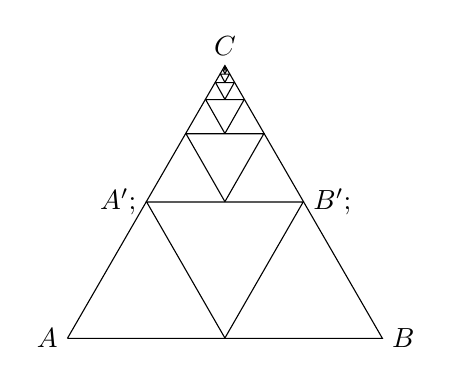
\begin{tikzpicture}[scale=2]
    \draw (0,0) node[left] {$A$} -- (2,0) node[right] {$B$} -- (1.5,0.866) node[right] {$B';$} -- (1, 1.732) node[above] {$C$} -- (0.5,0.866) node[left] {$A';$} -- (0,0);

    \foreach \x in {0,...,7}
    {
      \draw[line cap = round] (1, 1.734-1.732/2^\x) -- (1.003-0.5/2^\x,1.732-0.866/2^\x) -- (0.997+0.5/2^\x,1.732-0.866/2^\x) -- (1, 1.734-1.732/2^\x);
    }
  \end{tikzpicture}
  \begin{circuitikz}[scale=3]
    \draw (0,0) node[left] {$A$} to[R=$R/2$] (1,0) to[R=$R/2$] (2,0) node[right] {$B$} to[R=$R/2$] (1.5,0.866) node[right] {$B'$} to[R=$R_{AB}/2$] (0.5,0.866) node[left] {$A'$} to[R=$R/2$] (0,0);

    \draw (0.5,0.866) to[R=$R/2$] (1,0) to[R=$R/2$] (1.5,0.866);
  \end{circuitikz}
\end{figure}

Skeem on kesktelje suhtes sümmeetriline, seega on kogutakistus
\begin{align}
  R_{AB}&=2\left[\frac{1}{\frac{R}{2}}+\left(\frac{R}{2} + \frac{\frac{R}{2}\frac{R_{AB}}{4}}{\frac{R}{2}+\frac{R_{AB}}{4}}\right)^{-1}\right]^{-1}\\
        &= 2 \left[ \frac{1}{\frac{R}{2}} + \left( \frac{\frac{R}{2} \frac{R}{2} + \frac{R}{2} \frac{R_{AB}}{4} + \frac{R}{2}\frac{R_{AB}}{4}}{\frac{R}{2}+\frac{R_{AB}}{4}} \right)^{-1} \right]^{-1}\\
        &= 2 \left[ \frac{1}{\frac{R}{2}} +  \frac{\frac{R}{2}+\frac{R_{AB}}{4}}{\frac{R}{2}\left(\frac{R}{2}+ \frac{R_{AB}}{2}\right)}  \right]^{-1}\\
        &= 2 \left[ \frac{R+\frac{3}{4}R_{AB}}{\frac{R}{2}\left(\frac{R}{2}+ \frac{R_{AB}}{2}\right)}  \right]^{-1}\\
        &= \frac{2R(R + R_{AB})}{4R+3R_{AB}}.
\end{align}
Seega
\begin{align}
&4R R_{AB} +3 R_{AB}^2=2R^2+2R R_{AB}\\
  \implies& 3R_{AB}^2 +2 R R_{AB} - 2R^2=0 \\
  \implies& R_{AB}=\frac{-2R \pm \sqrt{4R^2+24R^2}}{6}=\frac{\pm\sqrt{7}-1}{3}R.
\end{align}
Kuna peab kehtima, et $R_{AB} \geq 0$, siis
\begin{equation}
R_{AB}= \frac{\sqrt{7}-1}{3} R.
\end{equation}
\probend
\bigskip

% L180
\setAuthor{Päivo Simson}
\setRound{piirkonnavoor}
\setYear{2021}
\setNumber{G 10}
\setDifficulty{10}
\setTopic{TODO}

\prob{Laeva vettelaskmine}
\solu
\textbf{Lahendus 1.} \\
Laevale mõjuvad raskusjõud $m\overrightarrow{g}$, kaldpinna toereaktsioon $\overrightarrow{N}$, hõõrdejõud $\overrightarrow{F}_h$ ja köie tõmbejõud $\overrightarrow{T}$. Et laev paigal püsiks, peab nende jõudude vektorsumma võrduma nulliga. Raskusjõud $m\overrightarrow{g}$ on konstantne suurus. Köie tõmbe kaldpinnaga ristuv komponent võib toereaktsiooni suurendada või vähendada ja vastavalt seosele $F_h=\mu N$ suureneb või väheneb samas proportsioonis ka hõõrdejõud. See tähendab, et vektori $\overrightarrow{N}+\overrightarrow{F}_h$ siht ei sõltu köie tõmbest $\overrightarrow{T}$, sest $\tan\gamma=F_h/N=\mu=\textit{const}$.

\begin{figure}[h]
\vspace{-0.0cm}
  \begin{center}
    \includegraphics[width=0.9\linewidth]{2021-v2g-10-yl1.pdf}
    %\caption{}
  \end{center}
  \vspace{-0.5cm}
\end{figure}

Vaatleme kõigepealt olukorda, kus köie tõmbejõud mõjub paralleelselt kaldpinnaga. Joonisel a) on sellele olukorrale vastavad jõud tähistatud primmiga. Nüüd on lihtne näha, et võimalikele tasakaaluolekutele vastavad vektordiagrammid saame, kui liigutame punkti A suvaliselt vektoriga $\overrightarrow{N}+\overrightarrow{F}_h$ määratud sihis. Sealjuures paneme tähele, et vektori $\overrightarrow{T}$ pikkus on minimaalne siis, kui see asetseb $\overrightarrow{N}+\overrightarrow{F}_h$ sihiga risti. Selline olukord on kujutatud joonisel b). Sarnaste kolmnurkade võrdlemine annab minimaalsele tõmbele vastava nurga $\beta$ väärtuseks $\beta=\gamma=\arctan\mu$. Samalt vektordiagrammilt saame ka minimaalse tõmbe
\[T_{min}=mg\sin(\alpha-\gamma)=\]
\[=mg\sin(\alpha-\arctan\mu)= mg\frac{\sin\alpha-\mu\cos\alpha}{\sqrt{1+\mu^2}}.\]


\emph{Märkus:} Kui lahendaja eeldab ekslikult, et $\overrightarrow{T}_{min}$ on paralleelne kaldpinnaga ja tuletab sellest lähtuvalt lõppvalemi $T$ jaoks, siis hinnata lahendust
maksimaalselt 4 p. vääriliseks.

\begin{wrapfigure}{r}{0.5\textwidth}
\vspace{-0.5cm}
  \begin{center}
    \includegraphics[width=0.8\linewidth]{2021-v2g-10-yl2.pdf}
  \end{center}
  \vspace{-0.5cm}
\end{wrapfigure}
\textbf{Lahendus 2.} \\
Olgu $\beta$ nurk kaldpinna sihi ja tõmbe $T$ sihi vahel. Valime ristkoordinaadistiku selliselt, et $x$-telg asetseb kaldpinna sihis. Kirjutame mõlema koordinaatelje jaoks välja jõudude tasakaalutingimused:
\begin{align*}
  F_x &= mg\sin{\alpha}-T\cos\beta-F_h=0,\\
  F_y &= N-T\sin\beta-mg\cos\alpha=0.
\end{align*}
Teisest võrrandist saame $N=T\sin\beta+mg\cos\alpha$
ja et $F_h =\mu N$, siis asendades need seosed esimesse võrrandisse saame
\[mg\sin\alpha-T\cos\beta-\mu T\sin\beta - \mu mg\cos\alpha=0,\]
millest
\[T=mg\frac{\sin\alpha-\mu\cos\alpha}{\cos\beta+\mu\sin\beta}.\]
Viimane valem annab tasakaalustava tõmbe $T$ suvalise nurga $\beta$ korral, kõik ülejäänud valemis esinevad parameetrid on ülesande tekstis fikseeritud suurused ehk konstandid.
Järelikult võime tõmmet $T$ vaadelda funktsioonina ühest muutujast $\beta$, st $T=T(\beta)$. Edasine ülesanne seisneb selle funktsiooni miinimumi leidmises. On selge, et $T$ on minimaalne siis,
kui nimetajas olev avaldis $\cos\beta+\mu\sin\beta$ on maksimaalne. Maksimumi määramiseks leiame selle avaldise tuletise $\beta$ järgi ja võrdsustame selle nulliga:
\[(\cos\beta+\mu\sin\beta)'=-\sin\beta+\mu\cos\beta=0, \]
millest $\mu=\tan\beta$ ehk $\beta=\arctan\mu$, mis ongi $T$ minimaalsele väärtusele vastav nurk. Asendades selle $T$ avaldisse saame
\[T_{min}=mg\frac{\sin\alpha-\mu\cos\alpha}{\cos(\arctan\mu)+\mu\sin(\arctan\mu)}= mg\frac{\sin\alpha-\mu\cos\alpha}{\sqrt{1+\mu^2}}.\]

\textbf{Hindamisskeem lahendusele 2.} \\
Õiged jõudude tasakaaluvõrrandid õpilase valitud koordinaatsüsteemis koos seletustega või joonisega, kus on näidatud võrranditele vastavad jõud ja nurgad [\textbf{4 p.}]\\
Korrektselt leitud $T$ üldavaldis [\textbf{2 p.}]\\
On aru saadud, et ülesanne taandub funktsiooni $T$ miinimumi leidmisele, ning et selleks tuleb kasutada tuletist. [\textbf{1 p.}]\\
Õigesti leitud tuletis ja sellest saadud miinimumile vastav seos $\mu=\tan\beta$, kus $\beta$ on nurk kaldpinna ja $\overrightarrow{T}_{min}$ vahel [\textbf{3 p.}]\\
Saadud õige lõppavaldis $T_{min}=mg\frac{\sin\alpha-\mu\cos\alpha}{\cos(\arctan\mu)+\mu\sin(\arctan\mu)}$ või sellega ekvivalentne avaldis, mis sisaldab ainult ülesande tekstis antud parameetreid
ja gravitatsioonikiirendust $g$ [\textbf{2 p.}]

\emph{Märkus:} Kui lahendaja eeldab ekslikult, et $\overrightarrow{T}_{min}$ on paralleelne kaldpinnaga ja tuletab sellest lähtuvalt lõppvalemi $T$ jaoks, siis hinnata lahendust
maksimaalselt 4 p. vääriliseks.
\probend
\bigskip

% L181
\setAuthor{Taavet Kalda}
\setRound{lõppvoor}
\setYear{2021}
\setNumber{G 10}
\setDifficulty{10}
\setTopic{TODO}

\prob{Sirgvool}
\solu
Olgu sirgvool piki $z-$telge. Ampère'i seadusest näeme et sirgvool tekitab magnetvälja tugevusega $B_\varphi = \frac{\mu_0}{2\pi r}I$. Elektronile mõjub Lorentzi jõud $\vec F = -e\vec v \times \vec B$. Selleks et $v_z = \mathrm{const}$, peab elektroni radiaalne kiiruskomponent olema $0$. Tõepoolest, kui see ei oleks 0, siis kruvireegli järgi oleks Lorentzi jõul $z-$sihiline komponent ning seega $v_z$ ei saaks konstantne olla. Kuna magnetväli tööd ei tee, on elektroni kiirus konstantne ning seega $v_\varphi = \mathrm{const}$. Tegu on liikumisega pikki heeliksit raadiusega $r$.

Näeme et Lorentzi jõule panustab ainult $z$-sihiline kiiruskomponent ning et kruvireegli järgi on $F = ev_z B$ radiaalsuunaline. Lorentzi jõudu tasakaalustab kesktõmbekiirendus kujul
\[
-\frac{m_ev_\varphi^2}{r} = ev_z B = ev_z \frac{I \mu_0}{2\pi r}.
\]
Paneme tähele, et selle võrrandi lahendamiseks peab $v_z$ olema negatiivne. Asendades $v_\varphi^2 = v_0^2 - v_z^2$, saame
\[
m_e(v_z^2 - v_0^2) = ev_z \frac{I\mu_0}{2\pi}.
\]
Tegu on ruutvõrrandiga, lahendiks saame
\[
v_z = \frac{e I\mu_0}{4\pi m_e} \pm \sqrt{\left(\frac{e I\mu_0}{4\pi m_e}\right)^2+v_0^2}.
\]
Kuna $v_z < v_0$, on positiivne lahend ebafüüsikaline, st
\[
|v_z| = v_0 \left(\sqrt{\left(\frac{e I\mu_0}{4\pi m_e v_0^2}\right)^2 + 1} - \frac{e I\mu_0}{4\pi m_e v_0^2}\right).
\]
\probend
\bigskip

% L182
\setAuthor{Marko Tsengov}
\setRound{lahtine}
\setYear{2022}
\setNumber{G 10}
\setDifficulty{10}
\setTopic{TODO}

\prob{Hantel ja pöörlemine}
\solu
Lahendus: vaatleme hõõrdejõust tekkivat jõumomenti hantli keskpunkti suhtes. Sümmeetria tõttu on mõlema raskuse tekitatud jõumoment $M$ sama, seega selleks, et nurkkiirendus oleks $0$, peab see jõumoment olema samuti $M = 0$.

Hantel pöörleb keskpunktist kaugusel $R$ joonkiirusega $v(R) = R \cdot \omega_v$, raskuse maad puudutav pind joonkiirusega $v_r = r \cdot \omega_s$. Normaaljõud on jaotunud ühtlaselt üle kokkupuutepinna maaga, seega on ka liugehõõrdejõu magnituud igas punktis sama ($\mu N \frac{dR}{d}$). Samas, kui $v > v_r$, on hõõrdejõud selles punktis suunatud hantli pöörlemise vastu. Juhul $v < v_r$ aga on hõõrdejõud suunatud pöörlemisega kaasa.

Eeldame, et $v > v_r$ parajasti siis, kui $R > k$. Olgu normaaljõud $N$ ning hõõrdetegur $\mu$ Sellisel juhul
\begin{gather*}
    M = \int\limits_{\ell / 2}^{k} \mu N R \frac{dR}{d} - \int\limits_{k}^{\ell/2 + d} \mu N R \frac{dR}{d} \\
    M = \frac{\mu N}{d} \left ( \int\limits_{\ell / 2}^{k} R \cdot dR - \int\limits_{k}^{\ell/2 + d} R \cdot dR \right ) \\
    0 = \frac{\mu N}{2 d} \left ( k^2 - \left ( \frac{\ell}{2} \right )^2 - \left ( \frac{\ell}{2} + d \right )^2 + k^2 \right ) \\
    0 = 2 k^2 - \frac{\ell^2}{2} - \ell d - d^2 \\
    k = \frac{1}{2} \sqrt{\ell^2 + 2 \ell d + 2 d^2} \\
    \left ( k = \sqrt{\frac{\left ( \frac{\ell}{2}\right )^2 + \left ( \frac{\ell}{2} + d \right )^2}{2}}\right )
\end{gather*}

$k$ tingimusest peab $v_r = v(k)$, seega
\begin{gather*}
    r \cdot \omega_s = k \cdot \omega_v \\
    \omega_v = \omega_s \frac{r}{k} = \omega_s \frac{2r}{\sqrt{\ell^2 + 2 \ell d + 2 d^2}}
\end{gather*}
\probend
\bigskip

% L183
\setAuthor{Jaan Kalda}
\setRound{piirkonnavoor}
\setYear{2022}
\setNumber{G 10}
\setDifficulty{10}
\setTopic{TODO}

\prob{Pingpong}
\solu
\emph{Märkus}: graafikult numbrite välja lugemise eest antakse punkte isegi siis, kui õpilane ei oska nendega midagi peale hakata.

\osa Teeme kindlaks esimese kuue põrke hetked sekundites: \num{0,92}; \num{1,93}; \num{2,78}; \num{3,49}; \num{4,1}; \num{4.61} (\p1; punkti teenimiseks piisab, kui välja on loetud esimesed kaks ja viimased kaks andmepunkti; kui on välja loetud vähem, kui neli andmepunkti, siis punkte ei anta; kui välja loetud andmepunktid ei sisalda esimest või kuuendat põrget, siis antakse \p{0,5}). Kuigi samplimise sagedus on $\SI{0.1}s$, siis graafikult on näha, et tulemusi saab välja lugeda täpsemalt --- ilmselt on graafikuid interpoleeritud (seda hindamisskeem ka eeldab: punkte ei alandata, kui välja loetud arvväärtused erinevad eeltoodutest mitte rohkem, kui $\SI{0.02}s$ võrra; kui ühes andmepunktis on suurem viga, mis pole siiski rohkem, kui  $\SI {0.04}s$, siis alandatakse skoori \p{0,5} võrra ja kui vigade arv on suurem, siis punkte ei anta).

Nende põhjal saame arvutada esimesele viiele põrkele järgnenud lennuajad sekundites: \num{1,01}; \num{0,85}; \num{0,71}; \num{0,61}; \num{0,51} (\p1; kui esimeses või viimases arvus on viga suurem, kui $\SI {0.03}s$, siis alandatakse skoori \p{0,5} võrra ja kui see on suurem, kui $\SI{0.05}s$, siis punkte ei anta).

Ülesande eelduste kohaselt peaks vähenema kineetiline energia geomeetrilise jadana: $T_n=mv_n^2/2=T_0k^n$ (valemina kirja panemise eest \p1). Kiirus $v_n$ on võrdeline ruutjuurega energiast, seega $v_n=v_0\sqrt{k^n}$ \p1 ning lennuaeg $t_n=2v_n/g$ on võrdeline kiirusega, seega $t_n=t_0\sqrt{k^n}$ \p1. Mõõdetud andmete kasutamise parim meetod oleks kanda need graafikule, kus horisontaalteljel on põrkenumber ja vertikaalteljel --- lennuaja logaritm $\ln t_n=\ln t_0 + \frac 12n\ln k$:  ning nimetatud teljestikus peaks tulema sirgjoon, mille kahekordne tõusunurga tangens annaks meile $\ln k$ väärtuse. Aga hea tulemuse saame ka, kui võtame viienda ja esimese lennuaja suhtest ruutjuure:  $k=\sqrt{0.51/1.01}\approx 0.71$, mis tähendab, et 29\% kineetilisest energiast kaob igal põrkel (ükskõik kumma meetodi rakendamine annab \p1). Õige numbrilise vastuse eest (vahemikus 25\% kuni 35\%) saab \p1, ebatäpse vastuse eest (vahemikus 20\% kuni 40\%) saab pooled punktid, st \p{0,5}. NB! Arvulise väärtuse eest saab punkte vaid siis, kui see tuleneb õige meetodi rakendamisest.

\osa Alates üheksandast põrkest on põrkeajad nii väiksed, et eelpooltoodud arvutuste läbiviimine on küll võimalik, kuid ebatäpne; kui viiakse läbi selline analüüs, siis saab selle ülesande osa (b) eest vaid kuni \p2: vastuse eest vastavalt allpooltoodud reeglile kuni \p1 ning kuni \p1 graafikult põrkehetkede välja lugemise eest (kui kasvõi ühes arvutusteks vajalikus andmes on viga suurem, kui $\SI{0.02}s$, siis \p{0,5} ning kui see on suurem, kui $\SI{0.04}s$, siis \p0).

Selle asemel kasutame teist meetodit: kuivõrd põrkeaegadest moodustub geomeetriline jada, siis palli seismajäämise hetke saab avaldada geomeetrilise jada summana. Kaheteistkümnes põrge toimub ajahetkel $\SI{6.97}s$ ja järgmine põrge --- ajahetkel $\SI{7.27}s$ (mõlemad andmepunktid kokku \p1; kui kasvõi ühes neist on viga suurem, kui $\SI {0.02}s$, siis alandatakse skoori \p{0,5} võrra ja kui see on suurem, kui $\SI {0.04}s$, siis punkte ei anta) ning põrked lõppevad ajahetkel $\SI{12.3}s$ (\p1; kui viga on suurem, kui $\SI {0.02}s$, siis alandatakse skoori \p{0,5} võrra ja kui see on suurem, kui $\SI {0.04}s$, siis punkte ei anta). Siit saame leida kaheteistkümnenda põrke kestvuse $t_{12}=\SI{0.3}s$.
Mõõtes nüüd ajavahemiku kaheteistkümnendast põrkest põrkumiste lõpuni $T=t_{12}/(1-\sqrt k)=\SI{5.33}s$ \p1 on lihtne leida $k=(1-t_{12}/T)^2\approx 0.88$ \p1, mis tähendab, et igal põrkel kaob 12\% kineetilisest energiat \p1. Kui vastus erineb antud numbrist rohkem, kui 1\% võrra, siis saab numbrilise vastuse eest vaid \p{0,5} punkti ning kui see erineb rohkem, kui 2\% võrra, siis punkte ei saa.

\emph{Märkus:} Tasub tähele panna, et saadud tulemus pole väga täpne, sest samplimise sagedus on ju vaid $\SI{0.1}s$, mistõttu $t_{12}$ leidmise suhteline viga on võrdlemisi suur. Seetõttu on täpsemateks arvutusteks vaja kasutada ka järgnevaid andmepunkte (põrgete hetked $\SI{7.58}s$, $\SI{7.88}s$, $\SI{8.17}s$ ja $\SI{8.39}s$) ning keskmistada. Geomeetrilises jadas on jada keskmine liige kõigi liikmete geomeetriline keskmine, aga kui keskmistatavad arvud erinevad üksteisest vähe, siis on geomeetriline keskmine ligikaudu võrdne aritmeetilise keskmisega. Seega me võime leida $t_{14}=(\num{8.39}-\num{6.97})\unit{s}/5= \SI{0.284}s$. Arvutades nüüd juba ajavahemiku neljateistkümnendast põrkest põrkumiste lõpuni $T'=t_{14}/(1-\sqrt k)=\SI{4.72}s$, saame tulemuseks $k=(1-t_{14}/T')^2\approx 0.88$, mis osutus võrdseks me esialgse tulemusega.
\probend
\bigskip

% L184
\setAuthor{Konstantin Dukats}
\setRound{lõppvoor}
\setYear{2022}
\setNumber{G 10}
\setDifficulty{10}
\setTopic{TODO}

\prob{Plaat}
\solu
\
Kui metallist plaat viiakse laengu elektrivälja, indutseerub selle peal laeng nii, et see kompenseerib välise elekrivälja (st plaadi sees paigutuvad laengud vastavalt ümber, kuni elektrivälja tugevus plaadis on null). Kuna $r \ll R$, saame eeldada, et laengute pindtihedused on mõlemal küljel on isotroopsed. Kuna plaadi kogulaeng on null, siis indutseeritud laeng plaadi pindadel on vastavalt $\pm \Delta q$. Plaat sarnaneb sellel juhul laetud kondensaatoriga. Kuna plaadi sees on elektrivälja tugevus null, siis peab välise elektrvälja ja indutseeritud elektrivälja summa olema $0$ ehk $\vec{E}_q + \vec{E}_{\pm \Delta q}=0$. Siit saame avaldada ümberpaigutunud laengu suuruse $\Delta q$:

$$\therefore \frac{1}{4\pi \varepsilon_0} \frac{q}{R^2} = \frac{\Delta q}{2 \pi r^2} - \frac{-\Delta q}{2 \pi r^2},$$
$$\frac{1}{4\pi \varepsilon_0} \frac{q}{R^2} = \frac{\Delta q}{\pi r^2},$$
\begin{equation}
\Delta q = \frac{1}{4\pi \varepsilon_0} \frac{q}{R^2} \pi r^2.
\end{equation}
Coulomb'i seadusest avaldame jõu, mis rakendub vastavalt kummalegi plaadi pinnale ning saame summarseks jõuks:
\begin{equation}
F = \frac{1}{4 \pi \varepsilon_0} \frac{q \Delta q}{R^2} - \frac{1}{4 \pi \varepsilon_0} \frac{q \Delta q}{(R+h)^2} \approx \frac{q \Delta q}{4 \pi \varepsilon_0} \frac{2Rh}{R^4},
\end{equation}
Võrranditest (1) ja (2) saame asendades:
$$F \approx \frac{q^2 h r^2}{8 \pi \varepsilon_0 R^5}.$$
\probend
\bigskip

% L185
\setAuthor{Uku Andreas Reigo}
\setRound{lahtine}
\setYear{2023}
\setNumber{G 10}
\setDifficulty{10}
\setTopic{TODO}

\prob{Kõver trajektoor}
\solu
Et trajektoor on kinnine ja ülesanne on mitmes mõttes sümmeetriline (näiteks laengu ja algse suuna vahetamise korral peaks töötama, lisaks ka olukorra peegeldamisel üle sirge y=x), siis on näha, et nurk kiirusvektori ja x-telje vahel, kui elektron lahkub 1. veerandist, on samuti $\alpha$.

Edaspidi annan kõik nurgad positiivse x-telje suhtes vastupäeva mõõdetuna. 

%TODO korruta -1-ga, et tuleks positiivne osa ringist.
Algne nurk on $\theta_1 = \frac{\pi}{2} - \alpha$. 1. sektorist väljudes on nurk $\theta_2 = \alpha - \pi$, ehk $\Delta\theta = 2\alpha - \frac{3\pi}{2}$, seega sealne trajektoori osa moodustab $\frac{2\alpha-\frac{3\pi}{2}}{2\pi} = \frac{\alpha}{\pi} - \frac{3}{4}$ ringist. Järeldub ka, et kesknurk sisenemis- ja väljumispunkti vahel 1. sektoris on $\gamma = \frac{\pi}{2} + 2\alpha$

Samuti sümmeetriast teame, et trajektoor lõikab x-telge punktis $(h,0)$. Seega on sisenemis- ja väljumispunkti ühendava kõõlu pikkus $L = \sqrt{2}h$ ning ringi raadius $R_2 = \frac{L}{2\sin{\frac{\gamma}{2}}} = \frac{\sqrt{2}h}{2\sin{(\frac{\pi}{4}+\alpha)}}$



\begin{figure}[h]
    \centering
    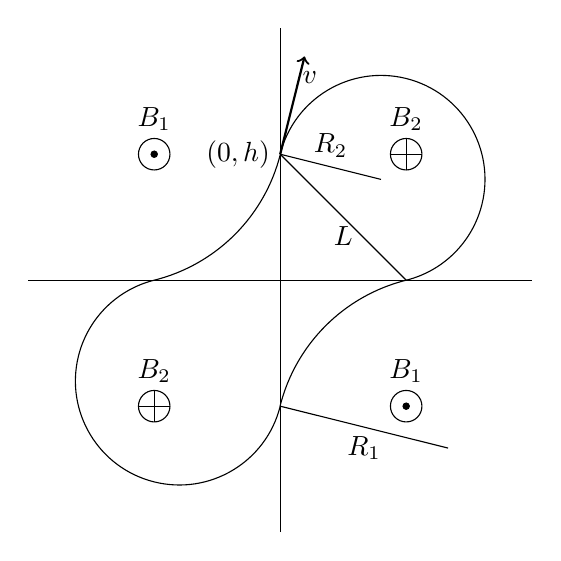
\begin{tikzpicture}[scale = 0.8]
        \draw (-4,0) -- (4,0);
        \draw (0,-4) -- (0,4);

        \draw[thick,->] (0,2) node [anchor = east] {$(0,h)$}
                            -- ++(76:1.6)
                            node [midway, yshift=10, anchor = west] {$\Vec{v}$};

        \draw (-2,2) circle (0.25) node[above, anchor = south, yshift = 5] {$B_1$};
        \filldraw (-2,2) circle (0.05);
        
        \draw (2,-2) circle (0.25) node[above, anchor = south, yshift = 5] {$B_1$};

        \filldraw (2,-2) circle (0.05);

        \draw (2,2) circle (0.25) node[above, anchor = south, yshift = 5] {$B_2$};
        \draw (2.25,2) -- (1.75,2);
        \draw (2,1.75) -- (2,2.25);

        \draw (-2,-2) circle (0.25) node[above, anchor = south, yshift = 5] {$B_2$};

        \draw (-2.25,-2) -- (-1.75,-2);
        \draw (-2,-1.75) -- (-2,-2.25);

        

        \draw (0,2) arc (166:-76:1.65);
        \draw (2,0) arc (104:166:2.75);
        \draw (0,-2) arc (-14:-256:1.65);
        \draw (-2,0) arc (-76:-14:2.75);

        \draw (0,2) -- (1.6,1.6) node[midway, above]{$R_2$};
        \draw (2.665,-2.665) -- (0,-2) node[midway, below]{$R_1$};
        \draw (0,2) -- (2,0) node [midway, below]{$L$};
    \end{tikzpicture}
    \caption*{Näidislahend $a = 14^\circ$ korral. $R_2 \approx 0.83 h$ ja $R_1 \approx 1.38 h$}
\end{figure}

2. sektoris viib sarnane arutelu arusaamani, et nurk muutub väärtuselt $\theta_2 = \alpha - \pi$ väärtuseni $\theta_3 = \frac{-\pi}{2} - \alpha$, läbides nurga $\Delta\theta = \frac{\pi}{2} - 2\alpha$. Seega kesknurk sisenemis- ja väljumispunkti vahel on $\gamma = \frac{\pi}{2} - 2\alpha$. Neid punkte ühendava kõõlu pikkus on jälle $L = \sqrt{2}h$ ning raadius $R_1 = \frac{L}{2\sin{\frac{\gamma}{2}}} = \frac{\sqrt{2}h}{2\sin{(\frac{\pi}{4}-\alpha)}}$

Et magnetväljas tiirleva elektroni tiirlemisraadius $R = \frac{mv}{qB}$, siis $\frac{R_1}{R_2} = \frac{B_2}{B_1} = \frac{\sin(\frac{\pi}{4}+\alpha)}{\sin{(\frac{\pi}{4}-\alpha)}}$
\probend
\bigskip

% L186
\setAuthor{Jaan Kalda}
\setRound{piirkonnavoor}
\setYear{2023}
\setNumber{G 10}
\setDifficulty{10}
\setTopic{TODO}

\prob{Alajaama kaugus}
\solu
\begin{center}
    \includegraphics[width=0.8\linewidth]{2023-v2g-10-yl.pdf}
\end{center}

Kõigepealt teeme ekvivalentskeemi: radiaatori (takistusega $R_r$) ja teiste tarbijate (takistusega $R_t$) rööpühendus on järjestikku mõlema juhtmega pingeallika külge, milleks on alajaam; olgu kummagi juhtme takistus $R_j$ ja pinge alajaamas $U_a$. Selles skeemis on teada pinge ühel juhtmel $U_1$ ja pinge radiaatoril $U_f$; kui eemaldada skeemist radiaator, siis tekkiva uue olukorra jaoks on teada uus pinge juhtmel $U_0$. Kummagi ekvivalentskeemi eest saab \p{1}.

Esimesest ekvivalentskeemist saame Kirchoffi pingeseaduse tõttu 
$$U_a=U_f+2U_1;$$
see võrrand annab \p{2} (kui puudub tegur 2, siis \p{1}). 
Teisest ekvivalentskeemist saame tänu Kirchoffi pingeseadusele avaldada uue faasipinge, st pinge teistel koormistel:
$$U_f'=U_a-2U_0=U_f+2(U_1-U_0)=\SI{210}{\V} + 2(30-20)\,\si{\V} = \SI{230}{\V}.$$
see võrrand annab samuti \p{2} (kui puudub tegur 2, siis \p{1}).

Selleks, et leida juhtme pikkus, on meil esimese sammuna vaja leida juhtme takistus. Peale pingete avaldamist on meil on alles jäänud kolm tundmatut takistit, millest radiaatori takistuse saame avaldada tänu nominaalandmetele: 
$$P_n=U_n^2/R_r\;\; \Rightarrow\;\; R_r=U_n^2/P_n=\SI{26.45}{\ohm}.$$
See seos (emb-kumb) annab \p{1}. Kahe tundmatu leidmiseks vajame kahte võrrandit, milleks on Ohmi ja Kirchoffi seadustest tulenev järeldus: jadaühenduses jagunevad pinged võrdeliselt takistustega. Seega
$$U_0/U_f'=R_j/R_t,\quad\p{1}$$
$$U_1/U_f=R_j(1/R_t+1/R_r).\quad\p{1}$$
Lahutades teisest võrrandist esimese saame
$$U_1/U_f-U_0/U_f'=R_j/R_r\Rightarrow R_j=R_r(U_1/U_f-U_0/U_f')=\SI{1.479}{\ohm}.\quad\p{1}$$
Et $R_j=\rho L/S$ \p{1}, siis $L=SR_j/\rho\approx\SI{1920}{\m}$. Numbrilise vastuse eest \p{1}.
\probend
\bigskip

% L187
\setAuthor{Jaan Kalda}
\setRound{lõppvoor}
\setYear{2023}
\setNumber{G 10}
\setDifficulty{10}
\setTopic{TODO}

\prob{Uppuv pall}
\solu
\par
Teeme joonise valguskiire käigu kohta silmast palli ülemise ja alumise servani. Need on veepinnal murduvad jooned, mis on peaaegu paralleelsed, kui vaadelda pallilähedast piirkonda, sest palli mõõtmed on hulga väiksemad kaugusest (mis on ilmselt suurem kõrgusest $H=\SI 2\m$). Alumiste sirgete osade vahekaugus $a$ on võrdne palli diameetriga, ülemiste sirgete osade vahekaugus $b$ vastab palli näivale kõrgusele. Ülaltvaates palli vasakusse ja paremasse serva tõmmatud sirged näiliselt ei murdu, seega pallin näiv laius on võrdne palli tegeliku laiusega. Seega on palli näiv lapikus $k=a/b=3$. Kui tähistada murdjoone ülemise osa kaldenurga veepinna suhtes $\beta$-ga ja alumise osa kaldenurga $\alpha$-ga, siis saame eelpooltoodud tingimusest johtuvalt seosed $a=d\sin\alpha$ ja $b=d\sin\beta$, kus $d$ tähistab murdjoonte murdepunktide kaugust. Seega saame võrrandi $\sin\alpha=k\sin\beta$ ning murdumisseadusest  $\cos\alpha=\cos\beta/n$. Võttes need avaldised ruutu ja liites vasakud ning paremad pooled saame $1-n^{-2}=(k^2-n^{-2})\sin^2\beta$, millest $\sin\beta=\sqrt{7/135}$. Silma kaugus pallist $L=H/\sin\beta=H\sqrt{135/7}\approx\SI{8.8}\m$.
\probend
\bigskip

% L188
\setAuthor{Jaan Kalda}
\setRound{lahtine}
\setYear{2024}
\setNumber{G 10}
\setDifficulty{10}
\setTopic{TODO}

\prob{Pärituul}
\solu
Kasutame ratturi kiirust kui ühikkiirust (st võtame selle võrdseks ühega). Takistusjõu ühikuks võtame takistusjõu siis, kui õhu kiirus ratturi suhtes on üks. Ratturi ja õhu suhtelise kiiruse ruudu leiame koosinusteoreemi abil $v^2=2-2\cos\alpha$, seega takistusjõu moodul  $f=2-2\cos\alpha$. Selle jõu teega risti oleva komponendi kompenseerimiseks rattur tööd ei pea tegema, piisab ratta õige kaldenurga hoidmisest. Kompenseerida tuleb teega risti olev komponent $f\cos\beta$, kus $\beta$ on suhtelise kiiruse nurk tee suhtes; selle leiame siinusteoreemist, $\sin\beta=\frac 1v\sin\alpha$. Seega saame kriitilise nurga väärtuse jaoks, mille puhul teesihiline takistusjõu komponent on 1, võrrandi
$$(2-2\cos\alpha)\sqrt{1-\sin^2\alpha/(2-2\cos\alpha)}=1.$$
See võrrand lihtsustub, kui läheme üle poolnurga siinusele kasutades seost $1-\cos\alpha=2\sin^2\frac\alpha 2$; lahendiks saame  $\sin\frac\alpha 2= 1/\sqrt[3]4$, millest $\alpha\approx 78.09^\circ$. Seega tuul takistab, kui nurk on suurem, kui $78.09^\circ$.
\probend
\bigskip

% L189
\setAuthor{Päivo Simson}
\setRound{piirkonnavoor}
\setYear{2024}
\setNumber{G 10}
\setDifficulty{10}
\setTopic{TODO}

\prob{Põrked}
\solu
\begin{wrapfigure}{r}{0.4\textwidth}
\vspace{-1.1cm}
  \begin{center}
    \includegraphics[width=1\linewidth]{2024-v2g-10-yl1.pdf}
  \end{center}
  \vspace{-1cm}
\end{wrapfigure}

\textbf{Lahendus 1}

Ilmselt on lihtsaim perioodiline liikumine selline, mille korral kummipall jääb põrkuma kahe punkti vahel, mis mõlemad on kera keskteljest kaugusel $a$ \p{1}. Uurime, kas selline lahend on võimalik, ja kui on, siis milline peab olema kaugus $a$. 

Kuni esimese põrkeni langeb pall vabalt kõrguse $h_0=\sqrt{R^2-a^2}$ võrra ja saavutab kiiruse $v_0=\sqrt{2gh_0}$ \p{1}. Elastne põrge toimub nurga $2\alpha$ all \p{1} ja edasi liigub pall mööda parabooli, mille haripunkt asub poolkera teljel \p{1}. Paraboolil liikudes on algkkiiruseks $\vec v_0$, mis on horisondi suhtes nurga $90^\circ-2\alpha$ all \p{1}. Kiiruse komponentide ajaline sõltuvus kahe põrke vahelisel ajal on
\begin{align*}
    &v_x=v_0\cos(90^\circ-2\alpha)=v_0\sin 2\alpha=const, \qquad\p{1}\\
    &v_y=v_0\sin(90^\circ-2\alpha)-gt=v_0\cos 2\alpha-gt. \qquad\p{1}
%    &x=v_{x}t=v_0t\sin 2\alpha\\
%    &y=v_{0y}t-gt^2/2
\end{align*}
Kui koordinaatide alguseks valida põrkekoht, siis on parabooli haripunktis $x=v_xt_h=a$, kus $t_h$ on haripunkti jõudmiseks kuluv aeg \p{1}. Lisaks on haripunktis $v_y=0$, millest saame
$t_h=v_0\cos 2\alpha/g$ \p{1}. Võrdus $a=v_xt_h$ annab nüüd
\[a=\frac{v_0^2\sin2\alpha\cos 2\alpha}{g}=2h_0\sin2\alpha\cos 2\alpha\qquad \p{1}\]
Jagame selle võrduse $h_0$-ga ja teisendame saadava võrduse paremat ja vasakut poolt:
\begin{align*}
a/h_0&=2\sin2\alpha\cos 2\alpha\\
\tan\alpha&=4\sin\alpha\cos\alpha(\cos^2\alpha-\sin^2\alpha)\\
\sin\alpha/\cos\alpha&=4\sin\alpha\cos\alpha(1-2\sin^2\alpha)\qquad \p{1}\\
\end{align*}
Saime võrrandi nurga $\alpha$ leidmiseks. Et $\alpha=0$ vastab juhule $a=0$, siis see lahend meile ei sobi. Korrutades viimast võrdust koosinusega ja jagades siinusega saame
\[1=4\cos^2\alpha(1-2\sin^2\alpha)=4(1-\sin^2\alpha)(1-2\sin^2\alpha)\]
Tähistame $x=\sin\alpha$, viime liikmed ühele poole võrdusmärki ja litsustame.
\[4(1-x^2)(1-2x^2)-1=0,\]
\[8x^4-12x^2+3=0.\qquad \p{2}\]
Saime ruutvõrrandi $x^2$ suhtes, mille lahend on
\[x^2=\frac{12\pm\sqrt{12^2-4\cdot8\cdot3}}{16}=\frac{12\pm\sqrt{48}}{16}=\frac{3\pm\sqrt{3}}{4}.\]
Plussiga lahend ei sobi, sest $\sin\alpha$ ei saa olla ühest suurem. Järelikult
\[x=\sin\alpha=\frac{\sqrt{3-\sqrt{3}}}{2},\]
ehk
\[a=R\frac{\sqrt{3-\sqrt{3}}}{2}\approx\num{0.563}R.\qquad \p{1}\]
Näeme, et kahe punkti vahel põrkuv liikumine on võimalik ja see realiseerub ülaltoodud $a$ väärtuse korral. Täpsemalt liigub pall ülevalt alla, siis mööda parabooli paremale, siis vertikaalselt üles ja alla, siis mööda parabooli tagasi esimese põrke punkti, uuesti üles ja alla jne.

\textbf{Lahendus 2}

Eeldame, et lihtsaim perioodiline liikumine on selline, mille korral kummipall jääb põrkuma kahe punkti vahel, mis mõlemad on kera keskteljest kaugusel $a$ \p{1}. Kuni esimese põrkeni langeb pall vabalt kõrguse $h_0$ võrra. Elastne põrge toimub nurga $2\alpha$ all \p{1} ja edasi liigub pall mööda parabooli, mille haripunkt asub eelduse põhjal poolkera teljel \p{1}.

\begin{wrapfigure}{r}{0.6\textwidth}
\vspace{-1.1cm}
  \begin{center}
    \includegraphics[width=1\linewidth]{2024-v2g-10-yl2.pdf}
  \end{center}
  \vspace{-0.5cm}
\end{wrapfigure}

Parabooli omadustest on teada, et vertikaalne kiir $CP$ peegeldub parabooli fookusesse $F$ \p{2}. Et langemisnurk ja peegeldumisnurk on võrdsed \p{1}, siis järelikult $\angle{FPB}=2\alpha$ \p{1}. Kolmnurgad $PAB$ ja $PBF$ on sarnased, järelikult lõik $PF=h_0$ \p{1} (seega on punkti $O$ läbiv horisontaaljoon parabooli juhtjooneks). Kolmnurgast $POA$ saame
\[\frac{a}{h_0}=\tan\alpha\qquad \p{1}\]
ja kolmnurgast $PCF$
\[\frac{a}{h_0}=\sin(180^\circ-4\alpha)=\sin(4\alpha). \qquad \p{1}\]
Tulemuseks on võrrand $\tan\alpha=\sin 4\alpha$, ehk
\[\frac{\sin\alpha}{\cos\alpha}=4\sin\alpha\cos\alpha(1-2\sin^2\alpha), \qquad \p{1}\]
mille lahendamisel saame (vt lahendus 1)
\[\sin\alpha=\frac{\sqrt{3-\sqrt{3}}}{2}=\frac{a}{R}. \qquad \p{3}\]
\probend
\bigskip

% L190
\setAuthor{Konstantin Dukatš}
\setRound{lõppvoor}
\setYear{2024}
\setNumber{G 10}
\setDifficulty{10}
\setTopic{TODO}

\prob{Kondensaator vedelikus}
\solu
\textit{Lahendus 1}:
Oletame, et kondensaatoril on ristkülikukujulised plaadid laiusega $L$ ja kõrgusega $H$ (tulemus ei sõltu kondensaatori kujust, kuid sellisel juhul on lahendus lihtsam). Kondensaatori vedeliku ja õhuga osi võib käsitleda paralleelsete kondensaatoritena. Olgu vedeliku tase kondensaatori sees $h$. Mahtuvused on siis:
\begin{align*}
C_1 &= \frac{\varepsilon_0 L (H-h)}{d},\\
C_2 &= \frac{\varepsilon_0 \varepsilon L h}{d}.
\end{align*}
Kondensaatori elektrostaatiline potentsiaalne energia on sellisel juhul $$E = E_1 + E_2 = \frac{C_ 1 V^2}{2} + \frac{C_ 2 V^2}{2} = \frac{\varepsilon_0 L H V^2}{2d} + \frac{\varepsilon_0 L (\varepsilon - 1) V^2}{2d}h = \frac{VQ}{2},$$
kus $Q$ on kondensaatori plaatide laeng. Edasi vaatleme kondensaatori ja pingeallika süsteemi summaarset potentsiaalset energiat $E_\mathrm{pot}$ sõltuvalt veetaseme kõrgusest. Kuna süsteem liigub madalaima potentsiaalse energiaga olekusse, kehtib tasakaaluasendis $\mathrm{d} E_\mathrm{pot} / \mathrm{d}h = 0$. Potentsiaalsesse energiasse panustub vee gravitatsiooniline potentsiaalne energia $mgh/2 = \rho L h^2 g/2$, kondensaatori elektrostaatiline potentsiaalne energia $E$ ning lõpuks pingeallika potentsiaalne energia. Pingeallika potentsiaalse energia arvutamiseks on kõige turvalisem kujutada pingeallikat ette kui hästi suure mahtuvusega $C_\infty$ kondensaatorit nõnda, et pingeallika potentsiaalne energia muut oleks $\mathrm{d}(C_\infty V^2/2) = \mathrm{d}(q^2/(2C_\infty)) = q\mathrm{d}q/C_\infty = V\mathrm{d}q$, kus $C_\infty$ on pingeallika mahtuvus ja $\mathrm{d}q$ on pingeallikasse sisenev laeng (teisisõnu negatiivse märgiga võrreldes kondensaatorisse siseneva laenguga). Pingeallika potentsiaalne energia on seega kondensaatori pinge kaudu avaldatav kui $-VQ$. (Alternatiivselt oleksime võinud otse $-VQ$ kirjutada kasutades ära asjaolu, et elektrivälja tehtud töö on $VQ$ mis on samas tõlgendatav kui negatiivne märk elektrivälja allikate potentsiaalse energia muuduga). Kokkuvõttes on potentsiaalne energia
\begin{align*}
E_\mathrm{pot} &=  \frac{\rho L h^2 g}{2} + \frac{VQ}{2} - VQ =\\
&=\frac{\rho L h^2 g}{2} -\frac{\varepsilon_0 L H V^2}{2d} - \frac{\varepsilon_0 L (\varepsilon - 1) V^2}{2d}h.
\end{align*}
Kuna süsteem läheb madalaima energiaga olekusse:
\[
\frac{\mathrm{d}E_\mathrm{pot}}{\mathrm{d}h} = -\frac{\varepsilon_0 L (\varepsilon - 1) V^2}{2d} + \rho L h g = 0.
\]
Millest
\[
  h = \frac{\varepsilon_0 (\varepsilon - 1) V^2}{2 \rho g d^2}.
\]
Nagu oodatud, taandusid kondensaatori plaatide laiusi ja kõrgusi kirjeldavad suurused ära.

\textit{Lahendus 2}: Nagu eelmiseski lahenduses eeldame lihtsuse mõttes, et kondensaatori plaadid on ristküliku kujulised laiusega (horisontaalsihis) $L$. Vedelikuga täidetud ja õhuga täidetud kondensaatoriosad on ühendatud rööbiti, seetõttu nende mahtuvused liituvad. Olgu vedelikuga täidetud kondensaatoriosa kõrgus $a$ ja õhuga täidetud osa kõrgus $b$. Sellisel juhul  kogumahtuvus $C=C_1+C_2= \frac{\varepsilon_0 L}{d}(\varepsilon a+b)$. Vaatleme olukorda, kus kondensaator on lahti ühendatud toitest ja seetõttu toiteallikas tööd ei saa teha. Sellisel juhul võtab süsteem madalaima potentsiaalse energiaga oleku, kus summaarne energia koosneb elektrostaatilisest osast $Q^2/2C$ ja gravitatsioonilisest osast $\frac 12\rho g h^2Ld$, kus $Q=VC$ säilib, sest plaadid on isoleeritud ja laeng ei saa neilt kuhugile ära minna. Niisiis on meie tingimus
$$0=\frac {\mathrm d}{\mathrm d h}\left( \frac 12\rho g h^2Ld+\frac 12\frac{Q^2}C\right)= \rho g hLd-\frac 12\frac{Q^2}{C^{2}} \frac{\mathrm dC}{\mathrm dh}.$$
Siinjuures
$$ \frac{\mathrm dC}{\mathrm dh}=\frac{\varepsilon_0 L}{d}(\varepsilon -1),$$
sest $\frac{\mathrm da}{\mathrm dh}=1$ ja $\frac{\mathrm db}{\mathrm dh}=-1$. Nüüd jääb üle vaid avaldada $h$ asendades $Q/C=V$, tulemuseks on eelpooltoodud vastus.

\textit{Lahendus 3}:
Seni kuni vahemaa vedeliku nivoost plaatide vahel kuni plaatide ülemise servani on palju suurem, kui $d$, siis servaefektid plaatide servades on tühised. Aga mingis mõttes tõusebki nivoo just servaefektide tõttu. Jõu ruumtihedus on võrdne elektrivälja tuletisega polarisatsioonivektori sihis, st $(\vec P\cdot\nabla)\vec E$-ga ning plaatide alumise serva juures on elektriväli servaefektist tingitult mittehomogeenne, mis annabki tõstejõu.

Teame, et $\nabla \times\vec E=0$, seega
\[
  0=\vec E\cdot(\nabla \times E)=\frac 12 \nabla E^2-(\vec E\times\nabla)\vec E,
\]
seega jõud ruumalaühiku kohta on
\[(\vec P \cdot \nabla)\vec E-\nabla p=(\varepsilon-1)\varepsilon_0(\vec E \cdot \nabla)\vec E-\nabla p=\nabla \left[\frac 12(\varepsilon-1)\varepsilon_0E^2-p \right].
\] Tasakaaluolekus on see kõik null, st $\frac 12(\varepsilon-1)\varepsilon_0E^2-p=\text{const}$. Plaatide vahelt väljas on $E=0$, seetõttu on sees rõhk  $\frac 12(\varepsilon-1)\varepsilon_0E^2$, kus $E=V/d$, mis kergitabki nivoo  $\frac 12(\varepsilon-1)\varepsilon_0V^2/\rho gd^2$ võrra kõrgemale.
\probend
\bigskip
\newpage

\section{Autorite loetelu}

TODO

\end{document}